\chapter{Sliding mode control}
The main idea behind \ac{SMC} is to force a system to a so called sliding manifold and let it slide along this surface to the origin. When on the sliding manifold, the system behaves like a system with an order of one less than the original. To keep the system on the sliding manifold, a rapid switching actuating signal is applied. This is obtained by the \textit{sign} function. As this would need infinite fast switching, which cannot be realised, often a boundary layer is introduced, where the \textit{sign} function is replaced with another function, like the \textit{tanh}.\\
Each joint of the robot is a second order system. This means, that the sliding surface has to be of first order. In order to stabilise the error system of the robot arm, the following sliding manifold is used for the $i^{th}$ joint:
\begin{gather*}
\mathbf{s} = \dot{\mathbf{e}} + \Lambda \mathbf{e}
\intertext{where:}
\begin{tabular}{>{$}l<{$} @{${}:{}$} l}
\Lambda & diagonal matrix with time constants of the systems, when in sliding mode
\end{tabular}\nonumber
\end{gather*}
This corresponds to a differential equation of first order. In order, that the system moves towards the origin, $\lambda > 0$ must be fulfilled. To control the robot, the following \ac{SMC} law is applied:
\begin{gather*}
\tau_c = \hat{\mathbf{M}}\ddot{\mathbf{q}}_s + \hat{\mathbf{V}}_m \dot{\mathbf{q}}_s + \hat{\mathbf{g}} + \mathbf{K} sign(\mathbf{s})
\intertext{where:}
\begin{tabular}{>{$}l<{$} @{${}:{}$} l}
\hat{\mathbf{M}} & estimated inertia matrix\\
\hat{\mathbf{V}}_m & estimated centrifugal/coriolis matrix\\
\dot{\mathbf{q}}_s & $\Lambda \mathbf{e} + \mathbf{\dot{q}}_D$\\
\hat{\mathbf{g}} & estimated gravitation vector\\
\mathbf{K} & diagonal matrix with gains
\end{tabular}\nonumber
\end{gather*}
The parameter matrix $\mathbf{K}$ is used to suppress the unknown or unmodelled dynamics of the system. This means, the better the dynamics are known or modelled, the lower $\mathbf{K}$ can be chosen.\\
To test the performance of the \ac{SMC} law, some simulation were done. For the first few simulations, the ideal sliding mode controller with the \textit{sign} function was used. For the last simulations, the \textit{sign} was replaced with the \textit{tanh} function, to show the effects of the boundary layer. For the simulations, the following reference signals were used:
\begin{align*}
	q_{D,1} = \sin(t)\\
	q_{D,2} = \cos(t)
\end{align*}
\section{Ideal sliding mode controller}
As estimated parameters, a portion of the actual parameters is used. The first three simulations use $\hat{\mathbf{M}} = 0.25\mathbf{M}$, $\hat{\mathbf{V}}_m = 0.75\mathbf{V}_m$ and $\hat{\mathbf{g}} = 0.75\mathbf{g}$. To show the influence of the controller parameters, the first simulation uses $\lambda_i = 10$ and $k_i = 20$. In the second simulation $\lambda_i = 10$ and $k_i = 10$ were applied. For the last simulation, $\lambda_i = 25$ and $k_i = 10$ was used.\\
Figure \ref{fig:ch6_sim1} shows the simulation results for the parameters $\lambda_i = 10$ and $k_i = 20$. The position error of the first joint converges to zero after approximately $1\,\mathrm{s}$ and for the second joint after $0.5\,\mathrm{s}$. The torques of both joints show the high frequency switching of the \ac{SMC} law.
\begin{figure}[H]
	\centering
	% This file was created by matlab2tikz v0.4.3.
% Copyright (c) 2008--2013, Nico Schlömer <nico.schloemer@gmail.com>
% All rights reserved.
% 
% The latest updates can be retrieved from
%   http://www.mathworks.com/matlabcentral/fileexchange/22022-matlab2tikz
% where you can also make suggestions and rate matlab2tikz.
% 
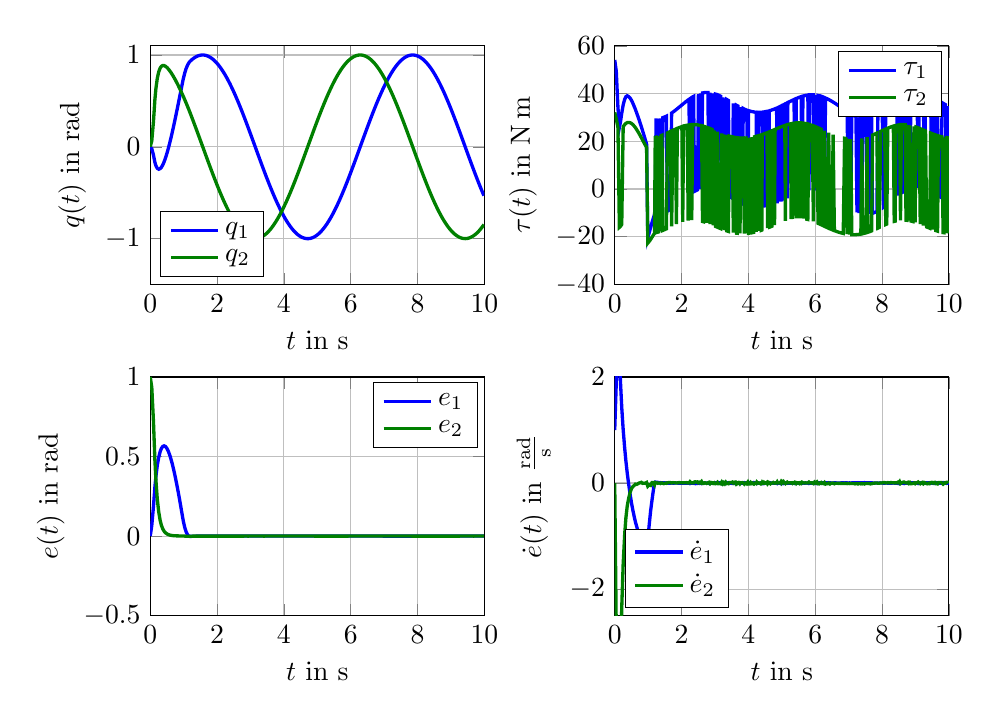
\begin{tikzpicture}

\begin{axis}[%
width=0.35\textwidth,
height=0.25\textwidth,
scale only axis,
xmin=0,
xmax=10,
xlabel={$t$ in $\mathrm{s}$},
xmajorgrids,
ymin=-1.5,
ymax=1.1,
ylabel={$q(t)$ in $\mathrm{rad}$},
ymajorgrids,
name=plot1,
legend style={at={(0.03,0.03)},anchor=south west,draw=black,fill=white,legend cell align=left}
]
\addplot [
color=blue,
solid,
line width=1.2pt
]
table[row sep=crcr]{
0 0\\
0.0465039723912261 -0.0209056940951578\\
0.0965039723912261 -0.0896498723409193\\
0.138996974223613 -0.168834260148198\\
0.170821418865936 -0.206930521141492\\
0.210324829147683 -0.233913195372513\\
0.253296278764971 -0.243890958475519\\
0.298845534220757 -0.237692724618603\\
0.335008469304094 -0.222650444271552\\
0.375746822327249 -0.196692632354422\\
0.41685468984732 -0.162158868463325\\
0.459681238418238 -0.118548737643306\\
0.502581803817871 -0.0681369543099867\\
0.542255344426739 -0.0164166249650618\\
0.58241112121378 0.0402922734746763\\
0.620082835590244 0.0968743063071986\\
0.658564450967407 0.157595071879779\\
0.692272387570107 0.2128342320388\\
0.728376983934156 0.273797312952363\\
0.760866520449888 0.32995183565099\\
0.798263179276667 0.395846010322051\\
0.833616194025603 0.459134575967961\\
0.872182950768084 0.528982200463543\\
0.911801555030177 0.601370413970454\\
0.953658066547812 0.678170238527388\\
0.990305195665215 0.742571483538954\\
1.03201791489503 0.803676408655357\\
1.07510399408218 0.853459451132998\\
1.11652681732679 0.889808095553981\\
1.15773451315211 0.915950428904952\\
1.19031924051665 0.930744553651141\\
1.21259548649245 0.938474119483589\\
1.23696551077686 0.94632765906469\\
1.26561095960737 0.955001067779739\\
1.29089068391975 0.962027662614007\\
1.31664863233206 0.9686363741998\\
1.3409199748277 0.97430423922076\\
1.36529056687226 0.97942916067903\\
1.38889569171686 0.983890104028348\\
1.41414069617504 0.988082742802179\\
1.44121464246057 0.991867348541476\\
1.4684773065876 0.994954247505671\\
1.49600474474772 0.997326580458069\\
1.52129093046682 0.998836738977445\\
1.54793979654979 0.999736131743772\\
1.5764441355025 0.999933155139716\\
1.61140374687881 0.999091219979867\\
1.65722943914053 0.996187425527815\\
1.70338479950607 0.991059039036004\\
1.7442957946018 0.984769180561429\\
1.78141131093847 0.977626567188053\\
1.81561188195195 0.969888176293376\\
1.84629396482328 0.961950742846319\\
1.87466337027942 0.953793481776368\\
1.90155077761943 0.945363699790223\\
1.92884877907911 0.936117816311143\\
1.95613210781287 0.92618801045527\\
1.98279994752652 0.915826177979296\\
2.00965948815797 0.904723005401139\\
2.0350160863527 0.893668551380135\\
2.06202157439872 0.881255198044476\\
2.08977149011476 0.867838923079045\\
2.11769605154001 0.853687637515212\\
2.14717290136877 0.837991373363179\\
2.17218212907013 0.824082220769336\\
2.19770468843464 0.809361781502553\\
2.22280000635272 0.794389292682846\\
2.25087797594372 0.777056875737667\\
2.27848095806415 0.759393493201217\\
2.30480721698826 0.74201795389523\\
2.33337523749106 0.722578330451405\\
2.36135361897641 0.702973909709455\\
2.38818541243229 0.683662802182292\\
2.41710333075832 0.662275804102901\\
2.44481341701625 0.641287479383237\\
2.47622453884958 0.616874230494522\\
2.50481900900832 0.594148100683275\\
2.5347492312302 0.569824050106188\\
2.56611131122929 0.543795074816347\\
2.59783749514547 0.516912248263253\\
2.62751093994745 0.491308285979794\\
2.65972756009095 0.462998285182064\\
2.69148543844692 0.434643778420562\\
2.72290515027316 0.406159660236397\\
2.75478872255641 0.376816948701064\\
2.78842505112561 0.345458422348503\\
2.82083749341136 0.314894118581919\\
2.85321965083216 0.284001016337834\\
2.88624672107291 0.252177908739203\\
2.91531714274161 0.223944886690348\\
2.94611519600364 0.193831375009004\\
2.97998736158042 0.160498495983444\\
3.01388315009216 0.126966518803487\\
3.04354463427037 0.0975059609448507\\
3.07596657903769 0.0651958630115041\\
3.10667884687011 0.0345261140360846\\
3.13677018529575 0.00444061707718587\\
3.17109557014923 -0.0298856250584617\\
3.20336421935897 -0.0621347236080901\\
3.23709503210224 -0.0957657971470984\\
3.26362199739017 -0.122130905584878\\
3.29267191913547 -0.150904586137348\\
3.3230569836985 -0.180873724232234\\
3.34971644839241 -0.207017694367864\\
3.37639558076311 -0.233039243796834\\
3.40302296717696 -0.258848560740954\\
3.42502995788466 -0.280021004602294\\
3.4459146040035 -0.299971182861285\\
3.46668444655047 -0.319689383067171\\
3.48733341188944 -0.339165140204702\\
3.51951370082286 -0.369294116695452\\
3.54877157370633 -0.39635591401563\\
3.57900629291898 -0.423955579139426\\
3.61117080188256 -0.452883827414921\\
3.64173390903776 -0.479926252476782\\
3.66721146574727 -0.502121424462294\\
3.68791303826267 -0.519923296416029\\
3.71183242179538 -0.540205210405117\\
3.7308225661396 -0.556064858676022\\
3.74961625894089 -0.571568810758041\\
3.76841305524083 -0.586885369505787\\
3.78699696005996 -0.601827489641816\\
3.80549629942339 -0.616496503441203\\
3.82379941145348 -0.630803543333694\\
3.84470118493509 -0.646891353731136\\
3.87836317914297 -0.672264825726859\\
3.90622942998247 -0.692660902583579\\
3.93076110587965 -0.710156361139792\\
3.95216888362504 -0.725081726896754\\
3.98230820836559 -0.745546247305536\\
4.00635534949041 -0.761366588239864\\
4.02973056293259 -0.776319592460551\\
4.05275502087946 -0.790633019358803\\
4.07366450777066 -0.803273236212189\\
4.09373957477731 -0.815068539891057\\
4.11516537249468 -0.827308132675911\\
4.13615815073306 -0.838924284784916\\
4.16078602371366 -0.852085828680035\\
4.18202303601144 -0.863023807837022\\
4.20676883808295 -0.875277086607789\\
4.23280237970251 -0.887600694858702\\
4.25347265790684 -0.896942653510799\\
4.27515056194439 -0.906347217547871\\
4.29628931402316 -0.91510576409278\\
4.31105524354128 -0.920948552032989\\
4.33177938796836 -0.928853566251348\\
4.34581027522694 -0.933948921378755\\
4.36297857162861 -0.939961290782512\\
4.38283244798352 -0.946576408484218\\
4.4025887691362 -0.952801974210381\\
4.41628689702606 -0.956867436587035\\
4.43235188588571 -0.961427677775136\\
4.44830824782228 -0.965714281956244\\
4.46490012882509 -0.969915455062273\\
4.4837604229187 -0.97437732554347\\
4.50196911777412 -0.978342673926487\\
4.52211702780986 -0.982374867868777\\
4.54091621378428 -0.985763361089657\\
4.55769329197907 -0.988483182063651\\
4.5759307305639 -0.991131061124132\\
4.5911108227051 -0.993077365957946\\
4.60903400546809 -0.995097208699435\\
4.62624939288257 -0.99672965191462\\
4.6422430557949 -0.997973268828757\\
4.65750020931939 -0.998916839569392\\
4.67334602680628 -0.999668030017544\\
4.68933042692808 -1.00016338968403\\
4.70605361468101 -1.00041142424573\\
4.72182992477807 -1.00038911027636\\
4.73956788104777 -1.00006888011241\\
4.75231829625489 -0.999616623423256\\
4.76804623406222 -0.99886589514464\\
4.78304501952076 -0.997921470127019\\
4.79933897392966 -0.996640378981631\\
4.81473454374285 -0.995181056844663\\
4.82933986519241 -0.993576593543459\\
4.84483207957565 -0.991653857909868\\
4.86173057734231 -0.989285832562819\\
4.87741045822504 -0.986833294198357\\
4.89443991794484 -0.983904591194858\\
4.90999672166107 -0.980966471644279\\
4.92576346365331 -0.977748266191281\\
4.94107871015708 -0.974389009478981\\
4.95693670109065 -0.970667130112769\\
4.9731799227112 -0.966609542044141\\
4.98932228320672 -0.962323959974478\\
5.00652181223338 -0.957477698369131\\
5.02268429356974 -0.952669896610415\\
5.03835501779681 -0.94776299862367\\
5.05585752006728 -0.942015503759712\\
5.07269954570595 -0.936213204339759\\
5.08988350260577 -0.930018014449448\\
5.10725019929574 -0.923476224379801\\
5.1247861165035 -0.916589365053644\\
5.14357949860555 -0.908895573844113\\
5.16306360210745 -0.90058171868714\\
5.18103702882289 -0.892598102268622\\
5.19995554436288 -0.883894934685919\\
5.21971548617572 -0.874463470239364\\
5.23992356210973 -0.864466107897254\\
5.25990166431111 -0.854236314173676\\
5.27996662714091 -0.843617576190126\\
5.30154702119995 -0.831817502479233\\
5.32194644901149 -0.820311980641251\\
5.34417903787342 -0.807386185656925\\
5.36682168329656 -0.793813253670978\\
5.38956363291842 -0.779769272160627\\
5.41068564313867 -0.766358459092138\\
5.43399214664186 -0.751180753510406\\
5.45604401678979 -0.73642909943078\\
5.47973644298944 -0.720179260776653\\
5.50374566919641 -0.703306684331017\\
5.52814444225204 -0.685742635443411\\
5.55475008845587 -0.666119326321913\\
5.58026245118698 -0.646864171243305\\
5.606320659161 -0.6267657882405\\
5.6328239175484 -0.605888411602271\\
5.66165116960789 -0.582706258569422\\
5.69233102797358 -0.557506869661316\\
5.72071349587992 -0.533703954236082\\
5.75025728493608 -0.508488825795637\\
5.77899205193103 -0.483518256754107\\
5.81132829466919 -0.454950193495413\\
5.84138566602952 -0.427969763249731\\
5.87324945833227 -0.398960857351821\\
5.90944716965074 -0.365510759984852\\
5.94564150355171 -0.331580255823723\\
5.98203104881769 -0.297037326357415\\
6.01770336168151 -0.262775408883792\\
6.05226882523353 -0.229273164004336\\
6.08423649476333 -0.198016519965919\\
6.11833223274655 -0.164483817366034\\
6.14985506441934 -0.133305169400996\\
6.18108557745708 -0.102290441997571\\
6.21185212003897 -0.0716301245977867\\
6.2433758214438 -0.0401487155437283\\
6.27679306940992 -0.0067454197651547\\
6.30846519231897 0.0249394417340443\\
6.33949674928634 0.055935550072485\\
6.37093691538187 0.0873017817970975\\
6.40266116628862 0.118862147171272\\
6.43976605774029 0.155600697281839\\
6.46758130157189 0.183021178005036\\
6.49998769885655 0.214774319239737\\
6.53544294467938 0.249271448713775\\
6.57369464205554 0.286132663715967\\
6.60512808134295 0.316137616318579\\
6.64453165519403 0.35327854531649\\
6.68381117067517 0.38977664990614\\
6.72321917685201 0.425779253123317\\
6.76236312889721 0.460897342923963\\
6.80070992981219 0.494612294546031\\
6.83895179043541 0.527480068654298\\
6.8778700464555 0.56017737227767\\
6.91636419154697 0.59167497755649\\
6.95501175824539 0.622421549469823\\
6.99211891365531 0.651122095129\\
7.02748810170113 0.67761549226303\\
7.06175198607126 0.702463753446509\\
7.09486305202876 0.725681829705672\\
7.12815804091614 0.748226137338166\\
7.15960181751857 0.768753221456551\\
7.19058786371548 0.788223841664327\\
7.21968885448527 0.805830630848881\\
7.2497707405396 0.823308685339552\\
7.2794529338125 0.839811601418996\\
7.30839614644494 0.855212270608964\\
7.33705264484543 0.869745156497276\\
7.36550816422365 0.883450853699041\\
7.39441714981722 0.896659406651951\\
7.42288928672357 0.908922774691065\\
7.45173608697344 0.920602477518643\\
7.47610245156088 0.929832881828229\\
7.49936104653973 0.938112867731174\\
7.52447318025858 0.946546486815394\\
7.55209944178396 0.955122738342868\\
7.57932047030006 0.962848490833963\\
7.60461720021986 0.969375421094698\\
7.63233272249048 0.97583028309395\\
7.65965107626739 0.981446324972429\\
7.68692656617411 0.986333129645686\\
7.71527146522864 0.990653233373858\\
7.74277289312236 0.994036766398008\\
7.76916782810323 0.996549869450864\\
7.79446609328887 0.998330153886008\\
7.81961912772421 0.999452811701242\\
7.84640342752329 0.999960350965752\\
7.87529164043463 0.999689319289283\\
7.91485268599895 0.998043311902617\\
7.96321538675132 0.993925864276753\\
8.00668041204966 0.988180718548991\\
8.04291295977839 0.981978580986174\\
8.07789489494143 0.974749323452602\\
8.11073709421044 0.966901623152265\\
8.14094856591195 0.958746279222325\\
8.17139102928635 0.94965496212791\\
8.19684195848291 0.941362160897857\\
8.22926462311873 0.929995811284938\\
8.25827793253431 0.918961798380733\\
8.28437436087312 0.908349034218659\\
8.31046698041353 0.897129430104977\\
8.33791383878077 0.884688621116247\\
8.36384893093362 0.872315107576371\\
8.39060975875072 0.858941200052595\\
8.41728751894939 0.845011032821736\\
8.44455555022826 0.830138007356535\\
8.47139912868571 0.81487114794461\\
8.49673461909071 0.799952619105627\\
8.52425013854956 0.783172905488794\\
8.55181363559815 0.765760303589109\\
8.57979073288858 0.747486808767647\\
8.60761830235697 0.728732052440309\\
8.63605298497665 0.708967782271093\\
8.66228633795453 0.690252402632718\\
8.68968364417766 0.67019228117869\\
8.71716815550259 0.649558859285417\\
8.74542530498622 0.627842934891488\\
8.77457913863047 0.604905175213083\\
8.80375379961273 0.581425956821051\\
8.83334720052184 0.557111249160932\\
8.8637214921041 0.531661372990317\\
8.89321458019384 0.506472819397815\\
8.92340798895609 0.480216495103506\\
8.95519622630286 0.452095056233942\\
8.98847632704607 0.422167522441461\\
9.01761988480744 0.395608464071966\\
9.04801234770838 0.367530744866382\\
9.08154669214192 0.336132313227016\\
9.11164277732313 0.307648835280978\\
9.14257888950433 0.278073214177887\\
9.17273414834419 0.248984242921738\\
9.20640515514054 0.216230647132033\\
9.23532963351545 0.187919900661922\\
9.26838682961974 0.1553623832564\\
9.30168334905255 0.122397677880888\\
9.33454052606865 0.0897393726224703\\
9.36349422948178 0.0608822108872148\\
9.39258143185908 0.0318272195916404\\
9.42434964154785 6.69246079354442e-05\\
9.45389289797482 -0.0294765432095621\\
9.48976403097997 -0.0653380132085312\\
9.5231071377822 -0.098579258741321\\
9.55346921818317 -0.128736809374395\\
9.58740370979129 -0.162331553140013\\
9.61121020166375 -0.185758630272936\\
9.63303236790917 -0.207125636422624\\
9.66090864193947 -0.234318714534953\\
9.68857850771103 -0.261137965730529\\
9.70981974529702 -0.281540660741153\\
9.73069704096935 -0.301474697803978\\
9.75146027547462 -0.321177078348003\\
9.77210280519362 -0.340636741761208\\
9.79486653425672 -0.361960647750154\\
9.82576176022772 -0.390626492257513\\
9.854767564631 -0.417188145261007\\
9.87842150449428 -0.438577604292315\\
9.89980992727215 -0.457707608002083\\
9.92695276788682 -0.481671367183075\\
9.94629392552653 -0.498503894770842\\
9.96546372040655 -0.515007140015918\\
9.98550208874494 -0.532061730403154\\
};
\addlegendentry{$q_1$};

\addplot [
color=green!50!black,
solid,
line width=1.2pt
]
table[row sep=crcr]{
0 0\\
0.0465039723912261 0.0649506414988492\\
0.0965039723912261 0.273900166389839\\
0.138996974223613 0.511959038561736\\
0.170821418865936 0.637535784933302\\
0.210324829147683 0.743854473925994\\
0.253296278764971 0.815723382207167\\
0.298845534220757 0.859175710283795\\
0.335008469304094 0.877104027519071\\
0.375746822327249 0.885240773527115\\
0.41685468984732 0.884193640613448\\
0.459681238418238 0.876152632705501\\
0.502581803817871 0.862880423446591\\
0.542255344426739 0.847227339704813\\
0.58241112121378 0.828597880809584\\
0.620082835590244 0.809127820168501\\
0.658564450967407 0.787421698664117\\
0.692272387570107 0.767118953629887\\
0.728376983934156 0.744138367152431\\
0.760866520449888 0.722536612328734\\
0.798263179276667 0.696598905851171\\
0.833616194025603 0.671045879593391\\
0.872182950768084 0.642148032317931\\
0.911801555030177 0.611328493818389\\
0.953658066547812 0.577822554353723\\
0.990305195665215 0.548023712176395\\
1.03201791489503 0.513272053467296\\
1.07510399408218 0.476426193898766\\
1.11652681732679 0.439942785992569\\
1.15773451315211 0.402781104585333\\
1.19031924051665 0.372521558502844\\
1.21259548649245 0.351518049709167\\
1.23696551077686 0.328385663088653\\
1.26561095960737 0.300894025771351\\
1.29089068391975 0.276593203055417\\
1.31664863233206 0.251631062940413\\
1.3409199748277 0.228003336345665\\
1.36529056687226 0.204214077163987\\
1.38889569171686 0.181001088990535\\
1.41414069617504 0.156061847735431\\
1.44121464246057 0.129270257569652\\
1.4684773065876 0.102206707253029\\
1.49600474474772 0.0748340709350326\\
1.52129093046682 0.0496590910572063\\
1.54793979654979 0.0231280234359103\\
1.5764441355025 -0.0053128666905893\\
1.61140374687881 -0.0402534964172258\\
1.65722943914053 -0.0861204065967055\\
1.70338479950607 -0.131992707070742\\
1.7442957946018 -0.172457324634478\\
1.78141131093847 -0.208869758451834\\
1.81561188195195 -0.242214293310641\\
1.84629396482328 -0.271822601130234\\
1.87466337027942 -0.298976259007123\\
1.90155077761943 -0.324464390699912\\
1.92884877907911 -0.350143512306183\\
1.95613210781287 -0.37552787531201\\
1.98279994752652 -0.400092221435933\\
2.00965948815797 -0.424517218565136\\
2.0350160863527 -0.447365977052863\\
2.06202157439872 -0.471371363021091\\
2.08977149011476 -0.495724308382629\\
2.11769605154001 -0.519861666291956\\
2.14717290136877 -0.544840878811202\\
2.17218212907013 -0.56559146321331\\
2.19770468843464 -0.586411243973071\\
2.22280000635272 -0.606544373142149\\
2.25087797594372 -0.628654801217069\\
2.27848095806415 -0.64985682737072\\
2.30480721698826 -0.66962684173743\\
2.33337523749106 -0.69058482038543\\
2.36135361897641 -0.710562227828359\\
2.38818541243229 -0.729183899482553\\
2.41710333075832 -0.748637022584458\\
2.44481341701625 -0.766708259676928\\
2.47622453884958 -0.786498443698435\\
2.50481900900832 -0.803834212513858\\
2.5347492312302 -0.821275860374399\\
2.56611131122929 -0.838799074914435\\
2.59783749514547 -0.855657700493139\\
2.62751093994745 -0.870644251046448\\
2.65972756009095 -0.886033701439024\\
2.69148543844692 -0.900320023349546\\
2.72290515027316 -0.913555585249186\\
2.75478872255641 -0.926045843979594\\
2.78842505112561 -0.938210201914293\\
2.82083749341136 -0.949008262455704\\
2.85321965083216 -0.958705525342459\\
2.88624672107291 -0.967577955132884\\
2.91531714274161 -0.974479463464043\\
2.94611519600364 -0.980931972912946\\
2.97998736158042 -0.98698446098729\\
3.01388315009216 -0.991901521072181\\
3.04354463427037 -0.995229392554582\\
3.07596657903769 -0.997903136264332\\
3.10667884687011 -0.999439480566434\\
3.13677018529575 -1.00005155817156\\
3.17109557014923 -0.99964428280462\\
3.20336421935897 -0.998175031416754\\
3.23709503210224 -0.995529837374419\\
3.26362199739017 -0.992597758873295\\
3.29267191913547 -0.988619837973511\\
3.3230569836985 -0.983585992452798\\
3.34971644839241 -0.978408760686456\\
3.37639558076311 -0.972545314646183\\
3.40302296717696 -0.965985184956781\\
3.42502995788466 -0.960070321126788\\
3.4459146040035 -0.954078900366738\\
3.46668444655047 -0.9477110209492\\
3.48733341188944 -0.940971402448923\\
3.51951370082286 -0.929598389561548\\
3.54877157370633 -0.918354736070007\\
3.57900629291898 -0.905917059255091\\
3.61117080188256 -0.891839941645072\\
3.64173390903776 -0.877597630825588\\
3.66721146574727 -0.865076828665713\\
3.68791303826267 -0.854461913842466\\
3.71183242179538 -0.841783829786211\\
3.7308225661396 -0.831403561172257\\
3.74961625894089 -0.820819791118375\\
3.76841305524083 -0.80992578731929\\
3.78699696005996 -0.798870349953072\\
3.80549629942339 -0.787592302398288\\
3.82379941145348 -0.776171618166583\\
3.84470118493509 -0.762838801982905\\
3.87836317914297 -0.740697755530118\\
3.90622942998247 -0.721679003903879\\
3.93076110587965 -0.7044838471369\\
3.95216888362504 -0.689097045972949\\
3.98230820836559 -0.666949223723707\\
4.00635534949041 -0.648861370136452\\
4.02973056293259 -0.630920942734611\\
4.05275502087946 -0.612898414861102\\
4.07366450777066 -0.596261446449529\\
4.09373957477731 -0.580038581373123\\
4.11516537249468 -0.562500474504885\\
4.13615815073306 -0.54503336299242\\
4.16078602371366 -0.52427337537462\\
4.18202303601144 -0.506078986962266\\
4.20676883808295 -0.484626589040117\\
4.23280237970251 -0.461736853574917\\
4.25347265790684 -0.443308929142687\\
4.27515056194439 -0.423772880102943\\
4.29628931402316 -0.404564368935089\\
4.31105524354128 -0.391014861944082\\
4.33177938796836 -0.371897456219625\\
4.34581027522694 -0.358867217647689\\
4.36297857162861 -0.342760230429438\\
4.38283244798352 -0.323992089553465\\
4.4025887691362 -0.305239802355187\\
4.41628689702606 -0.292197600603824\\
4.43235188588571 -0.276760348039766\\
4.44830824782228 -0.261331850163367\\
4.46490012882509 -0.245221803376385\\
4.4837604229187 -0.226857776961274\\
4.50196911777412 -0.209072124128408\\
4.52211702780986 -0.189317246133495\\
4.54091621378428 -0.170812552396195\\
4.55769329197907 -0.154238142958748\\
4.5759307305639 -0.136196731685479\\
4.5911108227051 -0.121110408467448\\
4.60903400546809 -0.103263181728603\\
4.62624939288257 -0.0861088587059517\\
4.6422430557949 -0.0701626283726122\\
4.65750020931939 -0.0549334001998756\\
4.67334602680628 -0.0390706761616778\\
4.68933042692808 -0.0230803031853161\\
4.70605361468101 -0.00636291060863052\\
4.72182992477807 0.00942988694340679\\
4.73956788104777 0.0271467888063226\\
4.75231829625489 0.0398222741584265\\
4.76804623406222 0.0555367794615217\\
4.78304501952076 0.0705415242418296\\
4.79933897392966 0.0867915913865901\\
4.81473454374285 0.102090755622321\\
4.82933986519241 0.11658463851208\\
4.84483207957565 0.131982331962568\\
4.86173057734231 0.148721609320193\\
4.87741045822504 0.164239139320601\\
4.89443991794484 0.181056333858661\\
4.90999672166107 0.196351552594777\\
4.92576346365331 0.211805882817269\\
4.94107871015708 0.22676155549994\\
4.95693670109065 0.24218161356078\\
4.9731799227112 0.257935053486449\\
4.98932228320672 0.273512274019066\\
5.00652181223338 0.29001525673793\\
5.02268429356974 0.305462252650193\\
5.03835501779681 0.320357150962347\\
5.05585752006728 0.336893988900006\\
5.07269954570595 0.352716932166002\\
5.08988350260577 0.36874601927545\\
5.10725019929574 0.384834210376212\\
5.1247861165035 0.400968762236363\\
5.14357949860555 0.418100056430577\\
5.16306360210745 0.435702304308596\\
5.18103702882289 0.451794564819065\\
5.19995554436288 0.468604540278258\\
5.21971548617572 0.48595956652899\\
5.23992356210973 0.503515242305445\\
5.25990166431111 0.520664176220058\\
5.27996662714091 0.537693340095382\\
5.30154702119995 0.55574686382537\\
5.32194644901149 0.572598712948225\\
5.34417903787342 0.590672109204406\\
5.36682168329656 0.608788720441625\\
5.38956363291842 0.626686715090296\\
5.41068564313867 0.643031791327898\\
5.43399214664186 0.660720953931224\\
5.45604401678979 0.677135077776796\\
5.47973644298944 0.694370895719241\\
5.50374566919641 0.711458477132364\\
5.52814444225204 0.728392329339373\\
5.55475008845587 0.746345063043133\\
5.58026245118698 0.763078853055129\\
5.606320659161 0.77967923214071\\
5.6328239175484 0.796007344558536\\
5.66165116960789 0.813115334778848\\
5.69233102797358 0.830581918830895\\
5.72071349587992 0.846050565825787\\
5.75025728493608 0.861435440315057\\
5.77899205193103 0.875671696435209\\
5.81132829466919 0.890803568768301\\
5.84138566602952 0.904068744703699\\
5.87324945833227 0.917234652487112\\
5.90944716965074 0.931008866650431\\
5.94564150355171 0.943572426218808\\
5.98203104881769 0.954959987171834\\
6.01770336168151 0.964879397324541\\
6.05226882523353 0.973370999203453\\
6.08423649476333 0.980200808499078\\
6.11833223274655 0.986365250935261\\
6.14985506441934 0.991059472598145\\
6.18108557745708 0.994739934684452\\
6.21185212003897 0.997409052741976\\
6.2433758214438 0.999169952156793\\
6.27679306940992 0.999957795095927\\
6.30846519231897 0.999643917563552\\
6.33949674928634 0.998384250091297\\
6.37093691538187 0.996096933906411\\
6.40266116628862 0.992792759165872\\
6.43976605774029 0.987673420689403\\
6.46758130157189 0.98299292330205\\
6.49998769885655 0.976519317367733\\
6.53544294467938 0.968239813197287\\
6.57369464205554 0.957951221817622\\
6.60512808134295 0.94844378159308\\
6.64453165519403 0.93517944682777\\
6.68381117067517 0.920513216115253\\
6.72321917685201 0.904359362478679\\
6.76236312889721 0.88693422951439\\
6.80070992981219 0.868531060307144\\
6.83895179043541 0.848944168005249\\
6.8778700464555 0.827692410795603\\
6.91636419154697 0.805455097883987\\
6.95501175824539 0.7819559602164\\
6.99211891365531 0.758297181448752\\
7.02748810170113 0.734822446644514\\
7.06175198607126 0.711190822581366\\
7.09486305202876 0.687563373400971\\
7.12815804091614 0.663026176057337\\
7.15960181751857 0.6391617081333\\
7.19058786371548 0.615063333858676\\
7.21968885448527 0.591863997452437\\
7.2497707405396 0.567354581576579\\
7.2794529338125 0.54269270789343\\
7.30839614644494 0.518135721637266\\
7.33705264484543 0.493407402911961\\
7.36550816422365 0.468492818601159\\
7.39441714981722 0.442759143506825\\
7.42288928672357 0.417081389220086\\
7.45173608697344 0.390691071720063\\
7.47610245156088 0.36823634394965\\
7.49936104653973 0.346615832340711\\
7.52447318025858 0.322930190362022\\
7.55209944178396 0.296659657141811\\
7.57932047030006 0.270587508932794\\
7.60461720021986 0.246212832964899\\
7.63233272249048 0.21928959517711\\
7.65965107626739 0.192617798209012\\
7.68692656617411 0.165824443903712\\
7.71527146522864 0.137798359552594\\
7.74277289312236 0.110603621437533\\
7.76916782810323 0.0844811070020451\\
7.79446609328887 0.0593355149739098\\
7.81961912772421 0.0343445959055751\\
7.84640342752329 0.00770004653517245\\
7.87529164043463 -0.0210335858657999\\
7.91485268599895 -0.0605653310227185\\
7.96321538675132 -0.108896653301739\\
8.00668041204966 -0.151995550358088\\
8.04291295977839 -0.187691325890267\\
8.07789489494143 -0.221881696028833\\
8.11073709421044 -0.253776519278406\\
8.14094856591195 -0.282852578222344\\
8.17139102928635 -0.311874821779099\\
8.19684195848291 -0.335921963381073\\
8.22926462311873 -0.366406720018528\\
8.25827793253431 -0.393204207930314\\
8.28437436087312 -0.41697698948198\\
8.31046698041353 -0.440484049246948\\
8.33791383878077 -0.464976219620261\\
8.36384893093362 -0.487756979642187\\
8.39060975875072 -0.510959766373023\\
8.41728751894939 -0.533727422401361\\
8.44455555022826 -0.556604429381131\\
8.47139912868571 -0.578649505412087\\
8.49673461909071 -0.599118538999179\\
8.52425013854956 -0.620956191820969\\
8.55181363559815 -0.642342974519128\\
8.57979073288858 -0.663519532023224\\
8.60761830235697 -0.684079735028346\\
8.63605298497665 -0.704513745048638\\
8.66228633795453 -0.722895153138865\\
8.68968364417766 -0.741553685708274\\
8.71716815550259 -0.759702410928815\\
8.74542530498622 -0.777795015646734\\
8.77457913863047 -0.795788671099719\\
8.80375379961273 -0.813104545194116\\
8.83334720052184 -0.829956892262611\\
8.8637214921041 -0.846546338979065\\
8.89321458019384 -0.861890653505814\\
8.92340798895609 -0.876803507631717\\
8.95519622630286 -0.891632752120822\\
8.98847632704607 -0.906206882412887\\
9.01761988480744 -0.91815991999798\\
9.04801234770838 -0.92975891589122\\
9.08154669214192 -0.941569456307312\\
9.11164277732313 -0.951261699039119\\
9.14257888950433 -0.960337025978186\\
9.17273414834419 -0.968302211250297\\
9.20640515514054 -0.97619626152456\\
9.23532963351545 -0.982046476322748\\
9.26838682961974 -0.987786972780703\\
9.30168334905255 -0.992461068879855\\
9.33454052606865 -0.995980416119629\\
9.36349422948178 -0.99815500158051\\
9.39258143185908 -0.99950120360216\\
9.42434964154785 -1.0000454860524\\
9.45389289797482 -0.99963118462875\\
9.48976403097997 -0.997933339059207\\
9.5231071377822 -0.995210260251041\\
9.55346921818317 -0.991767295885181\\
9.58740370979129 -0.986837664790332\\
9.61121020166375 -0.982672080876914\\
9.63303236790917 -0.978397742888441\\
9.66090864193947 -0.972233054443769\\
9.68857850771103 -0.965364707511348\\
9.70981974529702 -0.959698806438307\\
9.73069704096935 -0.953718960192484\\
9.75146027547462 -0.947360149524717\\
9.77210280519362 -0.94062751573066\\
9.79486653425672 -0.932629177827716\\
9.82576176022772 -0.920905504380464\\
9.854767564631 -0.909129971166025\\
9.87842150449428 -0.898964237106601\\
9.89980992727215 -0.889333759881617\\
9.92695276788682 -0.876631608158144\\
9.94629392552653 -0.867221293123026\\
9.96546372040655 -0.85757047884519\\
9.98550208874494 -0.847135972928143\\
};
\addlegendentry{$q_2$};

\end{axis}

\begin{axis}[%
width=0.35\textwidth,
height=0.25\textwidth,
scale only axis,
xmin=0,
xmax=10,
xlabel={$t$ in $\mathrm{s}$},
xmajorgrids,
ymin=-0.5,
ymax=1,
ylabel={$e(t)$ in $\mathrm{rad}$},
ymajorgrids,
name=plot3,
at=(plot1.below south west),
anchor=above north west,
legend style={draw=black,fill=white,legend cell align=left}
]
\addplot [
color=blue,
solid,
line width=1.2pt
]
table[row sep=crcr]{
0 0\\
0.0465039723912261 0.0673929065662346\\
0.0965039723912261 0.186004123949216\\
0.138996974223613 0.307384092596165\\
0.170821418865936 0.376922390962854\\
0.210324829147683 0.442690777163747\\
0.253296278764971 0.494487373310241\\
0.298845534220757 0.532109831307226\\
0.335008469304094 0.551427612631766\\
0.375746822327249 0.563659983100518\\
0.41685468984732 0.567045361363464\\
0.459681238418238 0.56221119494766\\
0.502581803817871 0.549826638550696\\
0.542255344426739 0.532485735876535\\
0.58241112121378 0.509746881233502\\
0.620082835590244 0.484228270338919\\
0.658564450967407 0.454387076143679\\
0.692272387570107 0.425453875075614\\
0.728376983934156 0.391862014227932\\
0.760866520449888 0.359597435966117\\
0.798263179276667 0.320298944566325\\
0.833616194025603 0.281232446607553\\
0.872182950768084 0.236752538932884\\
0.911801555030177 0.189237740657099\\
0.953658066547812 0.13736765463366\\
0.990305195665215 0.0936219138903973\\
1.03201791489503 0.0546596949919143\\
1.07510399408218 0.0261801678824202\\
1.11652681732679 0.00877371599198318\\
1.15773451315211 -5.43705242004311e-05\\
1.19031924051665 -0.00225698482148429\\
1.21259548649245 -0.00194501328178198\\
1.23696551077686 -0.00153360337265196\\
1.26561095960737 -0.0012097961005807\\
1.29089068391975 -0.000946152457105609\\
1.31664863233206 -0.000758439846002323\\
1.3409199748277 -0.00060966268626117\\
1.36529056687226 -0.000471257484699672\\
1.38889569171686 -0.000388457947301135\\
1.41414069617504 -0.000328162455844327\\
1.44121464246057 -0.000251313591318802\\
1.4684773065876 -0.000184273223428066\\
1.49600474474772 -0.000122167307745058\\
1.52129093046682 -6.18808663753745e-05\\
1.54793979654979 2.66914042745814e-06\\
1.5764441355025 5.08960310799944e-05\\
1.61140374687881 8.44120258673975e-05\\
1.65722943914053 7.95579009230662e-05\\
1.70338479950607 0.000163978787718233\\
1.7442957946018 0.000217504507618815\\
1.78141131093847 0.00027596306287192\\
1.81561188195195 0.000293870440249755\\
1.84629396482328 0.000339203535956067\\
1.87466337027942 0.000393077653621288\\
1.90155077761943 0.000433899989629838\\
1.92884877907911 0.00046330291076091\\
1.95613210781287 0.000484264343290075\\
1.98279994752652 0.0004941425699726\\
2.00965948815797 0.000512297503997394\\
2.0350160863527 0.00050261972781207\\
2.06202157439872 0.000500365175203132\\
2.08977149011476 0.000489021769400244\\
2.11769605154001 0.00045325912574401\\
2.14717290136877 0.000451505031898725\\
2.17218212907013 0.000470119059557184\\
2.19770468843464 0.000483284789002836\\
2.22280000635272 0.000480309016816727\\
2.25087797594372 0.000464500006241209\\
2.27848095806415 0.000475584209423174\\
2.30480721698826 0.000475720850138583\\
2.33337523749106 0.000478605014031075\\
2.36135361897641 0.000475422340216802\\
2.38818541243229 0.000465036777843264\\
2.41710333075832 0.000477310541677767\\
2.44481341701625 0.000463495035259553\\
2.47622453884958 0.000474536086582988\\
2.50481900900832 0.00045639096287986\\
2.5347492312302 0.000453277666485286\\
2.56611131122929 0.000443591654795794\\
2.59783749514547 0.000440942851043125\\
2.62751093994745 0.000427177569629844\\
2.65972756009095 0.000434414698054886\\
2.69148543844692 0.00041829475522881\\
2.72290515027316 0.000402015747746676\\
2.75478872255641 0.00041345652811936\\
2.78842505112561 0.000413219184620783\\
2.82083749341136 0.000389177060315438\\
2.85321965083216 0.00039177083701375\\
2.88624672107291 0.000402230994858144\\
2.91531714274161 0.000404654073605348\\
2.94611519600364 0.000403546501756474\\
2.97998736158042 0.000404292741110313\\
3.01388315009216 0.000396116698212351\\
3.04354463427037 0.000385037833640328\\
3.07596657903769 0.00038311548763928\\
3.10667884687011 0.000380599946051052\\
3.13677018529575 0.000381832524834752\\
3.17109557014923 0.000386988311123222\\
3.20336421935897 0.000402434243168173\\
3.23709503210224 0.000408527269946155\\
3.26362199739017 0.000404196130193171\\
3.29267191913547 0.000399394347759929\\
3.3230569836985 0.000403671322842608\\
3.34971644839241 0.000393147035131047\\
3.37639558076311 0.000387918954955324\\
3.40302296717696 0.000386031571130485\\
3.42502995788466 0.000363555135308002\\
3.4459146040035 0.000324832164118105\\
3.46668444655047 0.000293610889668061\\
3.48733341188944 0.000271446356673533\\
3.51951370082286 0.000305097372550855\\
3.54877157370633 0.000335439866829934\\
3.57900629291898 0.000357550192649214\\
3.61117080188256 0.000373691926749686\\
3.64173390903776 0.000376755338100387\\
3.66721146574727 0.000373042811807944\\
3.68791303826267 0.000376561180533641\\
3.71183242179538 0.000371316098379482\\
3.7308225661396 0.000343897659502712\\
3.74961625894089 0.000322416408074622\\
3.76841305524083 0.000312788244605233\\
3.78699696005996 0.000306019067560892\\
3.80549629942339 0.000300480886446741\\
3.82379941145348 0.000296137037529509\\
3.84470118493509 0.000299246933736397\\
3.87836317914297 0.000365291535007306\\
3.90622942998247 0.000385972800227341\\
3.93076110587965 0.000388615209796161\\
3.95216888362504 0.00039736308881122\\
3.98230820836559 0.000425711798309192\\
4.00635534949041 0.000425270995398574\\
4.02973056293259 0.000421213712389013\\
4.05275502087946 0.000416415194408049\\
4.07366450777066 0.000416391887039902\\
4.09373957477731 0.000406082937220109\\
4.11516537249468 0.000408031859306712\\
4.13615815073306 0.00040198584481077\\
4.16078602371366 0.000400246510100066\\
4.18202303601144 0.000401792171363047\\
4.20676883808295 0.000402809907751434\\
4.23280237970251 0.000414948681970562\\
4.25347265790684 0.000409585637615839\\
4.27515056194439 0.000422739217142531\\
4.29628931402316 0.000433371222058998\\
4.31105524354128 0.000407758683136139\\
4.33177938796836 0.000415213513286661\\
4.34581027522694 0.000389841734991792\\
4.36297857162861 0.000386571673359759\\
4.38283244798352 0.000390455402822676\\
4.4025887691362 0.00040747604741731\\
4.41628689702606 0.000386294811681287\\
4.43235188588571 0.000382491399892992\\
4.44830824782228 0.000381424223956706\\
4.46490012882509 0.000384820852715406\\
4.4837604229187 0.000399188225859382\\
4.50196911777412 0.000399369923414716\\
4.52211702780986 0.000422029727276341\\
4.54091621378428 0.000428829090021843\\
4.55769329197907 0.00042471738365446\\
4.5759307305639 0.000427049718889183\\
4.5911108227051 0.00042255210870179\\
4.60903400546809 0.000433581208654221\\
4.62624939288257 0.00043737271514499\\
4.6422430557949 0.000432485577666508\\
4.65750020931939 0.000422850000800779\\
4.67334602680628 0.000430109315788574\\
4.68933042692808 0.000429226348757084\\
4.70605361468101 0.000431492607908424\\
4.72182992477807 0.000433675660867494\\
4.73956788104777 0.000438203697478157\\
4.75231829625489 0.000413692647116992\\
4.76804623406222 0.000414360298950145\\
4.78304501952076 0.000416569782247245\\
4.79933897392966 0.000418148680598307\\
4.81473454374285 0.000413794045694971\\
4.82933986519241 0.000407557063969888\\
4.84483207957565 0.000411632131928075\\
4.86173057734231 0.000416578426254199\\
4.87741045822504 0.00041846686486835\\
4.89443991794484 0.000430145818053229\\
4.90999672166107 0.000427430227700976\\
4.92576346365331 0.000426363057192347\\
4.94107871015708 0.000424738196468155\\
4.95693670109065 0.000420201164508027\\
4.9731799227112 0.000423202060064742\\
4.98932228320672 0.000425543087161584\\
5.00652181223338 0.00042379548967586\\
5.02268429356974 0.000426456087394111\\
5.03835501779681 0.000421178581227144\\
5.05585752006728 0.000423220150156722\\
5.07269954570595 0.000425829954502577\\
5.08988350260577 0.000426961658323122\\
5.10725019929574 0.000426264805922227\\
5.1247861165035 0.000426697146141408\\
5.14357949860555 0.000426760491816447\\
5.16306360210745 0.000428258413412763\\
5.18103702882289 0.000418348731086482\\
5.19995554436288 0.000419451631633927\\
5.21971548617572 0.000416944105817607\\
5.23992356210973 0.000415309700386834\\
5.25990166431111 0.000414342281703006\\
5.27996662714091 0.000411892912594913\\
5.30154702119995 0.000408684686085015\\
5.32194644901149 0.000410531237744149\\
5.34417903787342 0.000414574350737995\\
5.36682168329656 0.000419878934615814\\
5.38956363291842 0.00042310051545047\\
5.41068564313867 0.00042006189719701\\
5.43399214664186 0.000433093296845266\\
5.45604401678979 0.000430014781021559\\
5.47973644298944 0.000424594170414294\\
5.50374566919641 0.000425744470541001\\
5.52814444225204 0.000424206594316523\\
5.55475008845587 0.000416542223190541\\
5.58026245118698 0.000413715420123473\\
5.606320659161 0.000413815043101562\\
5.6328239175484 0.000414348961557232\\
5.66165116960789 0.000423180758416519\\
5.69233102797358 0.000436194505459175\\
5.72071349587992 0.000425126424152822\\
5.75025728493608 0.000431336952842032\\
5.77899205193103 0.000417016207304499\\
5.81132829466919 0.000409036490800985\\
5.84138566602952 0.00040276048554716\\
5.87324945833227 0.000410364545505582\\
5.90944716965074 0.000412694841680661\\
5.94564150355171 0.000409757890632856\\
5.98203104881769 0.000414611672521603\\
6.01770336168151 0.000401049183265612\\
6.05226882523353 0.000403388665185495\\
6.08423649476333 0.000377532563323707\\
6.11833223274655 0.000376418224024067\\
6.14985506441934 0.000369609921318015\\
6.18108557745708 0.000368007142031765\\
6.21185212003897 0.000357417646354274\\
6.2433758214438 0.000349743954790177\\
6.27679306940992 0.000353225527289189\\
6.30846519231897 0.000337750877755113\\
6.33949674928634 0.000346136356910817\\
6.37093691538187 0.000337250151922625\\
6.40266116628862 0.000329672094629627\\
6.43976605774029 0.000341008259804376\\
6.46758130157189 0.00033162299777742\\
6.49998769885655 0.000333655687325712\\
6.53544294467938 0.000319331200104245\\
6.57369464205554 0.000307591302084242\\
6.60512808134295 0.000272499537314563\\
6.64453165519403 0.000255411132796479\\
6.68381117067517 0.000218074549653668\\
6.72321917685201 0.000190855340825302\\
6.76236312889721 0.000152408661522219\\
6.80070992981219 0.000118143221135347\\
6.83895179043541 0.000114511153116115\\
6.8778700464555 7.02716757129407e-05\\
6.91636419154697 3.54253327805587e-05\\
6.95501175824539 -4.98709276131049e-06\\
6.99211891365531 -9.7406778869269e-05\\
7.02748810170113 -0.000156353857993174\\
7.06175198607126 -0.000204023689229338\\
7.09486305202876 -0.000238872805421231\\
7.12815804091614 -0.000273122913210799\\
7.15960181751857 -0.000302510885802576\\
7.19058786371548 -0.000316933343336157\\
7.21968885448527 -0.000339628438359885\\
7.2497707405396 -0.000358029946946892\\
7.2794529338125 -0.000363082961250538\\
7.30839614644494 -0.000388653705124753\\
7.33705264484543 -0.000404147158163171\\
7.36550816422365 -0.000400598761156612\\
7.39441714981722 -0.000413647677554585\\
7.42288928672357 -0.000412934899784223\\
7.45173608697344 -0.000418262187031782\\
7.47610245156088 -0.000383680691078081\\
7.49936104653973 -0.000334566251790291\\
7.52447318025858 -0.000344975437233996\\
7.55209944178396 -0.000344166923649025\\
7.57932047030006 -0.00033133848918987\\
7.60461720021986 -0.000305953482555354\\
7.63233272249048 -0.000294001619849604\\
7.65965107626739 -0.00026915974879882\\
7.68692656617411 -0.000254406709691568\\
7.71527146522864 -0.000258073834124684\\
7.74277289312236 -0.000214088037798321\\
7.76916782810323 -0.000144404770127671\\
7.79446609328887 -0.000100680969717382\\
7.81961912772421 -4.31445278562537e-05\\
7.84640342752329 1.09345651609916e-05\\
7.87529164043463 8.36311154914782e-05\\
7.91485268599895 0.000104617586815903\\
7.96321538675132 0.000114059196796634\\
8.00668041204966 0.000183458714121287\\
8.04291295977839 0.000226921964391003\\
8.07789489494143 0.000286666344163078\\
8.11073709421044 0.000317374984292962\\
8.14094856591195 0.000360499842155915\\
8.17139102928635 0.000392187381592968\\
8.19684195848291 0.000434768077868131\\
8.22926462311873 0.000408122220339258\\
8.25827793253431 0.00041764276350964\\
8.28437436087312 0.000452928986163004\\
8.31046698041353 0.000477853634870296\\
8.33791383878077 0.000483638595967895\\
8.36384893093362 0.000494174989775109\\
8.39060975875072 0.000496204565043512\\
8.41728751894939 0.000483411151100732\\
8.44455555022826 0.000483230279576419\\
8.47139912868571 0.000505119413111599\\
8.49673461909071 0.000496031183134682\\
8.52425013854956 0.000481994560785126\\
8.55181363559815 0.000476748039806241\\
8.57979073288858 0.000475826091287601\\
8.60761830235697 0.000473089352805767\\
8.63605298497665 0.000487493168173425\\
8.66228633795453 0.000472920076012628\\
8.68968364417766 0.000464838424763081\\
8.71716815550259 0.000460418927859862\\
8.74542530498622 0.00044660021020182\\
8.77457913863047 0.00043949764390816\\
8.80375379961273 0.000442441546457228\\
8.83334720052184 0.000438080781713035\\
8.8637214921041 0.000419626804993967\\
8.89321458019384 0.000408799270267934\\
8.92340798895609 0.000410856599936116\\
8.95519622630286 0.000418277254970345\\
8.98847632704607 0.000422934234276084\\
9.01761988480744 0.000392870019251146\\
9.04801234770838 0.000384128869752809\\
9.08154669214192 0.00039932620279548\\
9.11164277732313 0.000394037448081475\\
9.14257888950433 0.000395193865480981\\
9.17273414834419 0.000399473476619061\\
9.20640515514054 0.0004107129032829\\
9.23532963351545 0.000397220630093231\\
9.26838682961974 0.000392019826391893\\
9.30168334905255 0.000386308522518447\\
9.33454052606865 0.000375647778965066\\
9.36349422948178 0.000363167095367392\\
9.39258143185908 0.00036374703159036\\
9.42434964154785 0.000361394600493624\\
9.45389289797482 0.000365719186016203\\
9.48976403097997 0.000397674753142507\\
9.5231071377822 0.000408456502590471\\
9.55346921818317 0.000400476680544354\\
9.58740370979129 0.000421687644722196\\
9.61121020166375 0.000404484397505428\\
9.63303236790917 0.000373297089725944\\
9.66090864193947 0.000376274441313995\\
9.68857850771103 0.00038646885800242\\
9.70981974529702 0.000343110682464065\\
9.73069704096935 0.000304987700306958\\
9.75146027547462 0.000274498341534035\\
9.77210280519362 0.000253126424960171\\
9.79486653425672 0.000262637719442516\\
9.82576176022772 0.00030219923950725\\
9.854767564631 0.000326792588042246\\
9.87842150449428 0.000334146220627052\\
9.89980992727215 0.000340733478547184\\
9.92695276788682 0.00033839107130712\\
9.94629392552653 0.000308745091261997\\
9.96546372040655 0.000283087305181895\\
9.98550208874494 0.000262150674312345\\
};
\addlegendentry{$e_1$};

\addplot [
color=green!50!black,
solid,
line width=1.2pt
]
table[row sep=crcr]{
0 1\\
0.0465039723912261 0.933968243634808\\
0.0965039723912261 0.721446937989837\\
0.138996974223613 0.478396424859677\\
0.170821418865936 0.347909679917309\\
0.210324829147683 0.234108675349788\\
0.253296278764971 0.152368264731274\\
0.298845534220757 0.0965013100997129\\
0.335008469304094 0.0673034976336249\\
0.375746822327249 0.0449930484157293\\
0.41685468984732 0.0301733140973106\\
0.459681238418238 0.0200413328949504\\
0.502581803817871 0.0134614322787215\\
0.542255344426739 0.0093196074983406\\
0.58241112121378 0.00654098685729265\\
0.620082835590244 0.00470250331130329\\
0.658564450967407 0.00344987782639949\\
0.692272387570107 0.00267861217316168\\
0.728376983934156 0.00211739338672756\\
0.760866520449888 0.00170216184199323\\
0.798263179276667 0.00135267097055025\\
0.833616194025603 0.00115697065545151\\
0.872182950768084 0.00100848742006043\\
0.911801555030177 0.000993926019734137\\
0.953658066547812 0.000881121821259767\\
0.990305195665215 0.000410971350785383\\
1.03201791489503 -0.000184211888857866\\
1.07510399408218 -0.000785425399670414\\
1.11652681732679 -0.00113676055675899\\
1.15773451315211 -0.00136559636149491\\
1.19031924051665 -0.00115807816478825\\
1.21259548649245 -0.000928213523282262\\
1.23696551077686 -0.000720907081861066\\
1.26561095960737 -0.000424043795355822\\
1.29089068391975 -0.000328238149387816\\
1.31664863233206 -0.000210490609852565\\
1.3409199748277 -0.000146206487277423\\
1.36529056687226 -0.000151773508067887\\
1.38889569171686 -0.000101912221065065\\
1.41414069617504 -4.61786350604565e-05\\
1.44121464246057 -5.09121536948765e-05\\
1.4684773065876 -6.61263534343787e-05\\
1.49600474474772 -0.000112197340231976\\
1.52129093046682 -0.00017391342578698\\
1.54793979654979 -0.000273483260625013\\
1.5764441355025 -0.000334911991667625\\
1.61140374687881 -0.000342764567505024\\
1.65722943914053 -0.00020512687863522\\
1.70338479950607 -0.000207629299603135\\
1.7442957946018 -0.000173003629962698\\
1.78141131093847 -0.00019157544049353\\
1.81561188195195 -0.000163090526535042\\
1.84629396482328 -0.000203241560490619\\
1.87466337027942 -0.000236056586937594\\
1.90155077761943 -0.000292287831367311\\
1.92884877907911 -0.000307350322298394\\
1.95613210781287 -0.000342441578885411\\
1.98279994752652 -0.000353867505495098\\
2.00965948815797 -0.000393414832341732\\
2.0350160863527 -0.000359292235617203\\
2.06202157439872 -0.000335247841154629\\
2.08977149011476 -0.000266195755581289\\
2.11769605154001 -0.000179994236681802\\
2.14717290136877 -0.00014860702185171\\
2.17218212907013 -0.000194219605456847\\
2.19770468843464 -0.000232573520325352\\
2.22280000635272 -0.000235913529904597\\
2.25087797594372 -0.000201708856015559\\
2.27848095806415 -0.000219310627824654\\
2.30480721698826 -0.000226233916567287\\
2.33337523749106 -0.000203619062807525\\
2.36135361897641 -0.0001831817515211\\
2.38818541243229 -0.000178219056472084\\
2.41710333075832 -0.00020094989617836\\
2.44481341701625 -0.000204829814254293\\
2.47622453884958 -0.00019113955584249\\
2.50481900900832 -0.000184132124009917\\
2.5347492312302 -0.00017637160775219\\
2.56611131122929 -0.000131359578027346\\
2.59783749514547 -0.000114275937413422\\
2.62751093994745 -0.000100392283520101\\
2.65972756009095 -9.84177631991878e-05\\
2.69148543844692 -8.04389359768676e-05\\
2.72290515027316 -6.77526866202927e-05\\
2.75478872255641 -7.35983012735142e-05\\
2.78842505112561 -7.16361190259418e-05\\
2.82083749341136 1.06631494830589e-05\\
2.85321965083216 -2.32515367737385e-06\\
2.88624672107291 1.9772314472366e-06\\
2.91531714274161 -2.92761370971339e-05\\
2.94611519600364 -2.30695154567195e-05\\
2.97998736158042 1.42017693833818e-05\\
3.01388315009216 4.53021180120139e-05\\
3.04354463427037 3.22500957882221e-05\\
3.07596657903769 5.57543571547692e-05\\
3.10667884687011 4.89056063892601e-05\\
3.13677018529575 6.3186249250613e-05\\
3.17109557014923 7.94622801840728e-05\\
3.20336421935897 8.22880057194109e-05\\
3.23709503210224 8.67244435109882e-05\\
3.26362199739017 3.41043879342751e-05\\
3.29267191913547 1.06193009455913e-05\\
3.3230569836985 5.51277516525062e-06\\
3.34971644839241 -1.15459504939075e-05\\
3.37639558076311 -1.48948263816173e-05\\
3.40302296717696 -3.60989780698873e-05\\
3.42502995788466 -2.95231381828298e-05\\
3.4459146040035 2.85534175482605e-05\\
3.46668444655047 8.96088255947225e-05\\
3.48733341188944 0.000146730009876195\\
3.51951370082286 0.000164635268578461\\
3.54877157370633 0.00011305543524065\\
3.57900629291898 6.67902412729848e-05\\
3.61117080188256 8.06819339789211e-05\\
3.64173390903776 8.27991594570809e-05\\
3.66721146574727 6.32094023405028e-05\\
3.68791303826267 1.98795849408739e-05\\
3.71183242179538 1.22654306417003e-05\\
3.7308225661396 3.46818612280142e-05\\
3.74961625894089 4.11626550345101e-05\\
3.76841305524083 2.91229771076651e-05\\
3.78699696005996 1.37167339537836e-05\\
3.80549629942339 -5.25011724650248e-07\\
3.82379941145348 -1.16144567983145e-05\\
3.84470118493509 2.87766673867651e-06\\
3.87836317914297 5.54559328211912e-05\\
3.90622942998247 4.51482724689312e-05\\
3.93076110587965 4.80822601772735e-05\\
3.95216888362504 1.60834930110765e-05\\
3.98230820836559 1.94016543807463e-05\\
4.00635534949041 4.06616889967459e-05\\
4.02973056293259 6.30301616026951e-05\\
4.05275502087946 7.07731029226943e-05\\
4.07366450777066 8.95857245676313e-05\\
4.09373957477731 0.000103170116026896\\
4.11516537249468 0.000151629685684052\\
4.13615815073306 0.000166081739268908\\
4.16078602371366 0.000220258673785279\\
4.18202303601144 0.000229940221129321\\
4.20676883808295 0.000276509068422637\\
4.23280237970251 0.000324400577777439\\
4.25347265790684 0.000332114614094658\\
4.27515056194439 0.000333581547414918\\
4.29628931402316 0.000368359899684867\\
4.31105524354128 0.000368413376040877\\
4.33177938796836 0.000410948840104342\\
4.34581027522694 0.000443662597675087\\
4.36297857162861 0.000416328466867066\\
4.38283244798352 0.000368632135044678\\
4.4025887691362 0.000371437533716545\\
4.41628689702606 0.000403451539599975\\
4.43235188588571 0.000369049795818699\\
4.44830824782228 0.000309870662759115\\
4.46490012882509 0.000251704529170976\\
4.4837604229187 0.000215794911792105\\
4.50196911777412 0.000201604055433041\\
4.52211702780986 0.000191299563884029\\
4.54091621378428 0.000178851009097925\\
4.55769329197907 0.000158714175381769\\
4.5759307305639 0.000161582604221278\\
4.5911108227051 0.000129333327892958\\
4.60903400546809 9.21191825472428e-05\\
4.62624939288257 7.57580555867249e-05\\
4.6422430557949 7.42145597670135e-05\\
4.65750020931939 7.21862559786082e-05\\
4.67334602680628 3.76410294668436e-05\\
4.68933042692808 2.37930345715238e-05\\
4.70605361468101 2.75872851450984e-05\\
4.72182992477807 1.0917203117411e-05\\
4.73956788104777 2.87658380278936e-05\\
4.75231829625489 9.64323383362276e-05\\
4.76804623406222 9.17434766813316e-05\\
4.78304501952076 5.57404938947986e-05\\
4.79933897392966 4.88822074451167e-05\\
4.81473454374285 7.62295707884969e-05\\
4.82933986519241 9.98290849562045e-05\\
4.84483207957565 7.39054319462418e-05\\
4.86173057734231 6.54809242042476e-05\\
4.87741045822504 3.43777679533419e-05\\
4.89443991794484 -9.33639450409474e-06\\
4.90999672166107 -2.73608662531566e-05\\
4.92576346365331 -4.68271564478817e-05\\
4.94107871015708 -5.99933855059132e-05\\
4.95693670109065 -6.40865899536325e-05\\
4.9731799227112 -9.02233498425997e-05\\
4.98932228320672 -0.000105186346352038\\
5.00652181223338 -0.000105224170578178\\
5.02268429356974 -0.000122392853145803\\
5.03835501779681 -0.000133048186382323\\
5.05585752006728 -0.00013892739841298\\
5.07269954570595 -0.000152058786436982\\
5.08988350260577 -0.000153460247615089\\
5.10725019929574 -0.000154119741590408\\
5.1247861165035 -0.000162118163929859\\
5.14357949860555 -0.000147409392339592\\
5.16306360210745 -0.000129408047550295\\
5.18103702882289 -0.000114050099090213\\
5.19995554436288 -0.000127143980424294\\
5.21971548617572 -0.000117338893434127\\
5.23992356210973 -0.000110615652732293\\
5.25990166431111 -9.90599142274284e-05\\
5.27996662714091 -0.000102254149500269\\
5.30154702119995 -8.56561675022238e-05\\
5.32194644901149 -9.4028892253295e-05\\
5.34417903787342 -8.18802419755293e-05\\
5.36682168329656 -7.94688900764839e-05\\
5.38956363291842 -9.31109559996202e-05\\
5.41068564313867 -0.000117822197932993\\
5.43399214664186 -0.000131860255084493\\
5.45604401678979 -0.000152546691452482\\
5.47973644298944 -0.00014238874294159\\
5.50374566919641 -0.000150959682384211\\
5.52814444225204 -0.000148791036554408\\
5.55475008845587 -0.000128068300176198\\
5.58026245118698 -0.000122885671688167\\
5.606320659161 -0.000138851100878301\\
5.6328239175484 -0.000142306081942767\\
5.66165116960789 -0.000129223399974676\\
5.69233102797358 -0.000116830533139822\\
5.72071349587992 -0.000111033821557527\\
5.75025728493608 -0.000112279108560043\\
5.77899205193103 -0.000107197736146314\\
5.81132829466919 -7.7832871494099e-05\\
5.84138566602952 -8.50843716926342e-05\\
5.87324945833227 -8.82603098097956e-05\\
5.90944716965074 -3.980012420568e-05\\
5.94564150355171 -1.49549936823146e-06\\
5.98203104881769 3.47589566278561e-05\\
6.01770336168151 8.67654872639401e-05\\
6.05226882523353 8.60496365078234e-05\\
6.08423649476333 7.40665530560847e-05\\
6.11833223274655 7.72266308896041e-05\\
6.14985506441934 6.52102878305749e-05\\
6.18108557745708 5.24141367067577e-05\\
6.21185212003897 4.78141168451796e-05\\
6.2433758214438 3.77549093921736e-05\\
6.27679306940992 2.17746217873183e-05\\
6.30846519231897 3.65631569962943e-05\\
6.33949674928634 3.06795710468544e-05\\
6.37093691538187 5.53637263546181e-05\\
6.40266116628862 7.84863740946884e-05\\
6.43976605774029 9.28393502704905e-05\\
6.46758130157189 5.42527604329157e-05\\
6.49998769885655 7.09545082357987e-05\\
6.53544294467938 0.000111591294895241\\
6.57369464205554 0.00014688396549345\\
6.60512808134295 0.000178713704211519\\
6.64453165519403 0.000242245050986023\\
6.68381117067517 0.000303874786435787\\
6.72321917685201 0.000377873792188455\\
6.76236312889721 0.000440058237380914\\
6.80070992981219 0.000515425185265483\\
6.83895179043541 0.000552129430966164\\
6.8778700464555 0.000632753282299503\\
6.91636419154697 0.000695507842150112\\
6.95501175824539 0.000730198392989156\\
6.99211891365531 0.000759374519652467\\
7.02748810170113 0.000737962697576977\\
7.06175198607126 0.000730010068748843\\
7.09486305202876 0.000718920635291997\\
7.12815804091614 0.000725500560223025\\
7.15960181751857 0.000747274006591026\\
7.19058786371548 0.000731034270862629\\
7.21968885448527 0.00074400539235675\\
7.2497707405396 0.000758275863632085\\
7.2794529338125 0.000746511209403389\\
7.30839614644494 0.000782946347840596\\
7.33705264484543 0.000805313922857875\\
7.36550816422365 0.000785613946234054\\
7.39441714981722 0.000798676309722468\\
7.42288928672357 0.000782070539703306\\
7.45173608697344 0.000794572786281866\\
7.47610245156088 0.000713764473577849\\
7.49936104653973 0.000618753025497965\\
7.52447318025858 0.00064777530573723\\
7.55209944178396 0.000658151875199242\\
7.57932047030006 0.000633307823788565\\
7.60461720021986 0.000575268332385998\\
7.63233272249048 0.00054889901279212\\
7.65965107626739 0.000491938582588614\\
7.68692656617411 0.00045469541604376\\
7.71527146522864 0.000467427829048489\\
7.74277289312236 0.000376034251874671\\
7.76916782810323 0.000231052422480296\\
7.79446609328887 0.000144896938454646\\
7.81961912772421 1.11483067369855e-05\\
7.84640342752329 -0.000121912618842403\\
7.87529164043463 -0.000274807760484882\\
7.91485268599895 -0.000268137199615055\\
7.96321538675132 -0.00011999928262571\\
8.00668041204966 -0.000110508374006169\\
8.04291295977839 -0.000118018854947832\\
8.07789489494143 -0.00016518776160282\\
8.11073709421044 -0.000167194256133207\\
8.14094856591195 -0.000191917135818009\\
8.17139102928635 -0.000231592299284489\\
8.19684195848291 -0.000260345153885289\\
8.22926462311873 -0.000129117953568847\\
8.25827793253431 -0.000167681255097973\\
8.28437436087312 -0.000250756089981707\\
8.31046698041353 -0.000312008105171291\\
8.33791383878077 -0.000287222567035006\\
8.36384893093362 -0.000304447092572269\\
8.39060975875072 -0.000281221365730944\\
8.41728751894939 -0.000256795727848536\\
8.44455555022826 -0.000233392240079788\\
8.47139912868571 -0.000281874485210443\\
8.49673461909071 -0.000282794208297243\\
8.52425013854956 -0.000240232531492302\\
8.55181363559815 -0.000215023416487825\\
8.57979073288858 -0.000221303585736465\\
8.60761830235697 -0.000215421452017139\\
8.63605298497665 -0.000236715860324699\\
8.66228633795453 -0.000222077031263979\\
8.68968364417766 -0.000213816899652497\\
8.71716815550259 -0.00021530695325378\\
8.74542530498622 -0.000184585680770843\\
8.77457913863047 -0.000174787259810572\\
8.80375379961273 -0.000178411089384878\\
8.83334720052184 -0.000186917375519013\\
8.8637214921041 -0.000147117743509284\\
8.89321458019384 -0.00012502190642838\\
8.92340798895609 -0.000121431456307275\\
8.95519622630286 -0.000124884804566072\\
8.98847632704607 -0.000113869819231116\\
9.01761988480744 -9.00151492952972e-05\\
9.04801234770838 -0.000100560418896833\\
9.08154669214192 -0.000102703025585904\\
9.11164277732313 -0.000110777208133461\\
9.14257888950433 -0.000108363266716149\\
9.17273414834419 -0.00010253987153841\\
9.20640515514054 -5.49976920668493e-05\\
9.23532963351545 -6.17976614850635e-05\\
9.26838682961974 -8.8390753318901e-06\\
9.30168334905255 2.7649106575045e-05\\
9.33454052606865 4.90514674013065e-05\\
9.36349422948178 3.22617955821336e-05\\
9.39258143185908 1.94670667386099e-05\\
9.42434964154785 4.55777810725033e-05\\
9.45389289797482 5.49944738070796e-05\\
9.48976403097997 4.41906858522634e-05\\
9.5231071377822 4.06799342973496e-05\\
9.55346921818317 3.65936727843019e-05\\
9.58740370979129 3.21138050851655e-05\\
9.61121020166375 2.94059571470662e-07\\
9.63303236790917 4.43231218061335e-06\\
9.66090864193947 -1.73941151576651e-05\\
9.68857850771103 -4.12469341056765e-05\\
9.70981974529702 4.89026499561618e-05\\
9.73069704096935 0.000148403958667109\\
9.75146027547462 0.000247941734535906\\
9.77210280519362 0.000340860284234412\\
9.79486653425672 0.000333865418700174\\
9.82576176022772 0.000228065599653382\\
9.854767564631 0.000159887693710892\\
9.87842150449428 0.000107924085788191\\
9.89980992727215 5.56582235521352e-05\\
9.92695276788682 9.37789075244888e-05\\
9.94629392552653 0.000156363123120729\\
9.96546372040655 0.000214572840551042\\
9.98550208874494 0.000265730801151998\\
};
\addlegendentry{$e_2$};

\end{axis}

\begin{axis}[%
width=0.35\textwidth,
height=0.25\textwidth,
scale only axis,
xmin=0,
xmax=10,
xlabel={$t$ in $\mathrm{s}$},
xmajorgrids,
ymin=-2.5,
ymax=2,
ylabel={$\dot{e}(t)$ in $\mathrm{\frac{rad}{s}}$},
ymajorgrids,
name=plot2,
at=(plot3.right of south east),
anchor=left of south west,
legend style={at={(0.03,0.03)},anchor=south west,draw=black,fill=white,legend cell align=left}
]
\addplot [
color=blue,
solid,
line width=1.2pt
]
table[row sep=crcr]{
0 1\\
0.0465039723912261 1.88925298244227\\
0.0965039723912261 2.86934761255994\\
0.138996974223613 2.4815515552857\\
0.170821418865936 1.92793603986872\\
0.210324829147683 1.4252292528491\\
0.253296278764971 1.00583587069693\\
0.298845534220757 0.654044283409986\\
0.335008469304094 0.41308531821516\\
0.375746822327249 0.181219913387048\\
0.41685468984732 -0.0169695306595368\\
0.459681238418238 -0.208821743334971\\
0.502581803817871 -0.376562812709288\\
0.542255344426739 -0.510272158527915\\
0.58241112121378 -0.630100625856166\\
0.620082835590244 -0.73503622826453\\
0.658564450967407 -0.821654520874161\\
0.692272387570107 -0.896000089894831\\
0.728376983934156 -0.970099492749281\\
0.760866520449888 -1.02701839337303\\
0.798263179276667 -1.08770915720865\\
0.833616194025603 -1.12887137452343\\
0.872182950768084 -1.17696918851907\\
0.911801555030177 -1.21866669292053\\
0.953658066547812 -1.26365106300129\\
0.990305195665215 -1.06087991252801\\
1.03201791489503 -0.787872369882617\\
1.07510399408218 -0.520938225857941\\
1.11652681732679 -0.318517773332151\\
1.15773451315211 -0.130326139350819\\
1.19031924051665 0.0100305106479084\\
1.21259548649245 0.0183221705981692\\
1.23696551077686 0.0154783582129646\\
1.26561095960737 0.0120762173432353\\
1.29089068391975 0.0119559164885125\\
1.31664863233206 0.00746776896714638\\
1.3409199748277 0.00543247115495746\\
1.36529056687226 0.00787819447776555\\
1.38889569171686 0.00304454816285446\\
1.41414069617504 0.00189895786965452\\
1.44121464246057 0.0051389032519475\\
1.4684773065876 0.00685368363740725\\
1.49600474474772 0.00378834891630529\\
1.52129093046682 0.00151569627109424\\
1.54793979654979 0.00303541604885127\\
1.5764441355025 -0.000847991971117779\\
1.61140374687881 -0.00351748893957434\\
1.65722943914053 -0.00293929964985451\\
1.70338479950607 0.000954616611890086\\
1.7442957946018 -0.00185341929360308\\
1.78141131093847 -0.00149412947990818\\
1.81561188195195 0.000564815328038204\\
1.84629396482328 0.00124880840016062\\
1.87466337027942 -0.000260397883646513\\
1.90155077761943 -0.00172273955536217\\
1.92884877907911 -0.00249385386954853\\
1.95613210781287 -0.00097772434803145\\
1.98279994752652 -0.00380662523754399\\
2.00965948815797 -0.000722799647092209\\
2.0350160863527 -0.00276031679723088\\
2.06202157439872 -0.00161823390398491\\
2.08977149011476 -0.00348344721522115\\
2.11769605154001 -0.000908902245184806\\
2.14717290136877 -0.00167816126315312\\
2.17218212907013 -0.00319549140276643\\
2.19770468843464 -0.000276730731484709\\
2.22280000635272 -0.00224426824726587\\
2.25087797594372 -0.0101509215770692\\
2.27848095806415 -0.00432926997853522\\
2.30480721698826 -0.0019917871489612\\
2.33337523749106 -0.00134198512619099\\
2.36135361897641 -0.00290439874338611\\
2.38818541243229 -0.00898943373652272\\
2.41710333075832 -0.0111149375436091\\
2.44481341701625 -0.00885287902778398\\
2.47622453884958 -0.00985376921266556\\
2.50481900900832 -0.00239449264140634\\
2.5347492312302 -0.00654203996615854\\
2.56611131122929 -0.00238983055223818\\
2.59783749514547 -0.0107346804930178\\
2.62751093994745 0.00172692576216826\\
2.65972756009095 0.00184798177556345\\
2.69148543844692 0.000713366649884195\\
2.72290515027316 0.000266561204402938\\
2.75478872255641 0.00205724582611166\\
2.78842505112561 -0.00158452268524079\\
2.82083749341136 -0.00814640303272496\\
2.85321965083216 0.00530034304381022\\
2.88624672107291 -0.00407173382368398\\
2.91531714274161 -0.00514411716768748\\
2.94611519600364 0.00306330171933344\\
2.97998736158042 -0.0045150931964727\\
3.01388315009216 0.00339890368387519\\
3.04354463427037 0.00396708910409149\\
3.07596657903769 -0.00512521486050366\\
3.10667884687011 0.00655390136591716\\
3.13677018529575 0.00384702667973058\\
3.17109557014923 0.00667625365764701\\
3.20336421935897 -0.00919282424689827\\
3.23709503210224 0.00761132160320244\\
3.26362199739017 -0.00461612702185754\\
3.29267191913547 0.00486180109153223\\
3.3230569836985 -0.00759354867332662\\
3.34971644839241 0.00428493149796427\\
3.37639558076311 0.00351536133814168\\
3.40302296717696 0.00370336373614788\\
3.42502995788466 -0.00391639275434097\\
3.4459146040035 -0.00361770565587993\\
3.46668444655047 -0.00322556767048754\\
3.48733341188944 -0.00276888138431886\\
3.51951370082286 -0.00792676950896509\\
3.54877157370633 0.000525653512013502\\
3.57900629291898 -0.00775549559202149\\
3.61117080188256 -0.00878878734215427\\
3.64173390903776 0.00828773513303749\\
3.66721146574727 0.00432142258641566\\
3.68791303826267 -0.0037103679624193\\
3.71183242179538 -0.00631746219207829\\
3.7308225661396 -0.00608798862979743\\
3.74961625894089 0.00378249102623929\\
3.76841305524083 -0.00367215337143367\\
3.78699696005996 -0.00352243672630181\\
3.80549629942339 -0.00355116818893486\\
3.82379941145348 -0.00360723083149328\\
3.84470118493509 0.00527658369583284\\
3.87836317914297 0.0089156277202227\\
3.90622942998247 0.00277444360893664\\
3.93076110587965 5.75578475914273e-06\\
3.95216888362504 0.00287343085794611\\
3.98230820836559 -0.00568073904906652\\
4.00635534949041 0.00800114740554969\\
4.02973056293259 0.00824438435274477\\
4.05275502087946 0.00746195346393319\\
4.07366450777066 -0.00396811856463508\\
4.09373957477731 0.00301400674409524\\
4.11516537249468 -4.82784983620865e-05\\
4.13615815073306 0.00333347918149862\\
4.16078602371366 0.00925497302196165\\
4.18202303601144 -0.00176787749079266\\
4.20676883808295 -0.00148596948385948\\
4.23280237970251 0.00401224265223848\\
4.25347265790684 -0.00819190696113759\\
4.27515056194439 -0.0049584385251068\\
4.29628931402316 -0.00183961895604923\\
4.31105524354128 -0.00107996077145345\\
4.33177938796836 0.00214660639455866\\
4.34581027522694 0.00160628412359354\\
4.36297857162861 -0.00150153762050725\\
4.38283244798352 0.00544102182124839\\
4.4025887691362 0.00387002247398738\\
4.41628689702606 -0.00595305583940237\\
4.43235188588571 0.000498697084279465\\
4.44830824782228 0.00142843444491469\\
4.46490012882509 -0.00701492797639364\\
4.4837604229187 0.00235183482142068\\
4.50196911777412 0.0021524976462079\\
4.52211702780986 0.00047137107218434\\
4.54091621378428 -0.00422362480794072\\
4.55769329197907 -0.00822351249152101\\
4.5759307305639 0.00453261354596016\\
4.5911108227051 -0.00127149595714297\\
4.60903400546809 -0.00508179885681301\\
4.62624939288257 -0.00209536846135086\\
4.6422430557949 0.00214316827325085\\
4.65750020931939 0.00365881656280336\\
4.67334602680628 -0.000906143264912097\\
4.68933042692808 -0.000757639755540801\\
4.70605361468101 0.00135164000322081\\
4.72182992477807 -0.000922103398669098\\
4.73956788104777 -0.00302796704903823\\
4.75231829625489 -0.00039044387674448\\
4.76804623406222 -0.00163652960624856\\
4.78304501952076 0.00106414756385778\\
4.79933897392966 -0.00232854054964304\\
4.81473454374285 0.00146940822550233\\
4.82933986519241 -0.00162238326691361\\
4.84483207957565 -0.00209021436409529\\
4.86173057734231 -0.0089040022386164\\
4.87741045822504 -0.00109908675116968\\
4.89443991794484 0.000686398201929062\\
4.90999672166107 -0.0017211750396916\\
4.92576346365331 -0.000379571443315407\\
4.94107871015708 -0.00234788343780962\\
4.95693670109065 -0.00194154702702576\\
4.9731799227112 -0.00933644419825558\\
4.98932228320672 -0.00122195091582311\\
5.00652181223338 -0.0087639588856796\\
5.02268429356974 -0.00237704369041436\\
5.03835501779681 -0.000782364617929021\\
5.05585752006728 -0.00858956930200311\\
5.07269954570595 -0.00183468775670254\\
5.08988350260577 -0.000425853507943164\\
5.10725019929574 0.00291213150227215\\
5.1247861165035 -0.00163057857891791\\
5.14357949860555 -0.00105161313702989\\
5.16306360210745 -0.00510042526833776\\
5.18103702882289 -0.00146273749344811\\
5.19995554436288 -0.000412108961087621\\
5.21971548617572 -0.00320577149062518\\
5.23992356210973 -7.47752150428438e-05\\
5.25990166431111 -0.00272655086811213\\
5.27996662714091 -0.000840390810432301\\
5.30154702119995 -0.00132431557786572\\
5.32194644901149 0.0017649028284118\\
5.34417903787342 -0.00275187733334004\\
5.36682168329656 -0.000453723939296435\\
5.38956363291842 -0.0086322815706199\\
5.41068564313867 -0.00527288445783702\\
5.43399214664186 0.00277398260335837\\
5.45604401678979 -0.00398407200462869\\
5.47973644298944 -0.00254858021479798\\
5.50374566919641 -0.00334217242775381\\
5.52814444225204 0.00455246486234062\\
5.55475008845587 -0.00305403129380688\\
5.58026245118698 0.00280022016318138\\
5.606320659161 -0.00569067789620825\\
5.6328239175484 -0.000853850992896144\\
5.66165116960789 -0.000748990710099151\\
5.69233102797358 -0.00264154909236503\\
5.72071349587992 0.00065761702445355\\
5.75025728493608 -0.00102817361735574\\
5.77899205193103 0.00132163027497501\\
5.81132829466919 -0.00838029310867627\\
5.84138566602952 -0.00284291686280158\\
5.87324945833227 -0.00226026992656359\\
5.90944716965074 -0.00202888426794268\\
5.94564150355171 0.00514939794059455\\
5.98203104881769 -0.00831045813874365\\
6.01770336168151 2.4176070308024e-05\\
6.05226882523353 -0.00938275658323062\\
6.08423649476333 0.00477159829599794\\
6.11833223274655 0.00641244590901024\\
6.14985506441934 1.47113383531794e-05\\
6.18108557745708 -0.00663558004305265\\
6.21185212003897 0.00563990113517232\\
6.2433758214438 0.00543987064725904\\
6.27679306940992 -0.00489655286253798\\
6.30846519231897 0.00629487202236889\\
6.33949674928634 0.00312875655049549\\
6.37093691538187 0.00366905657334282\\
6.40266116628862 0.000813582210359876\\
6.43976605774029 0.0060561686473396\\
6.46758130157189 0.00116342305778649\\
6.49998769885655 -0.0011832933878182\\
6.53544294467938 -0.000873895204182906\\
6.57369464205554 0.00467011339320644\\
6.60512808134295 0.00327327413207978\\
6.64453165519403 0.00192755780892206\\
6.68381117067517 0.00221052541730515\\
6.72321917685201 0.00138494900790165\\
6.76236312889721 0.00252753887052526\\
6.80070992981219 0.00323974658659765\\
6.83895179043541 0.00386375779647175\\
6.8778700464555 0.00229059074455207\\
6.91636419154697 0.00287498814057174\\
6.95501175824539 0.00310314532165767\\
6.99211891365531 0.000903707465811809\\
7.02748810170113 0.00288663653360532\\
7.06175198607126 0.00143288875069791\\
7.09486305202876 0.00302978409457444\\
7.12815804091614 0.00345723259932695\\
7.15960181751857 0.00337334585038129\\
7.19058786371548 0.0060362811513055\\
7.21968885448527 0.00473352749537992\\
7.2497707405396 0.00314950056289343\\
7.2794529338125 0.0069470418051667\\
7.30839614644494 0.00360543472410124\\
7.33705264484543 0.00414317014511506\\
7.36550816422365 0.00667341029628415\\
7.39441714981722 0.00302632830920457\\
7.42288928672357 0.00635343934965626\\
7.45173608697344 0.00523274728376433\\
7.47610245156088 0.00777589185604588\\
7.49936104653973 0.00380697608978053\\
7.52447318025858 0.00345064527953987\\
7.55209944178396 0.00308616692832575\\
7.57932047030006 0.00385568311981388\\
7.60461720021986 0.00275579043162455\\
7.63233272249048 0.0066695636201729\\
7.65965107626739 0.00645917267382914\\
7.68692656617411 0.0058052925396147\\
7.71527146522864 0.00217264843147433\\
7.74277289312236 0.00129992699308046\\
7.76916782810323 0.00112757440454898\\
7.79446609328887 0.00060518627562834\\
7.81961912772421 -0.000458742945952495\\
7.84640342752329 -0.000585017607668596\\
7.87529164043463 0.00216598271525589\\
7.91485268599895 0.00198660235226278\\
7.96321538675132 0.000588493854165623\\
8.00668041204966 0.00096051520134155\\
8.04291295977839 -0.00245787836201075\\
8.07789489494143 -0.00314749967141126\\
8.11073709421044 0.000659037455444211\\
8.14094856591195 -0.000322887558708129\\
8.17139102928635 -0.00173713347729015\\
8.19684195848291 -0.00414648546545759\\
8.22926462311873 -0.00226733930819201\\
8.25827793253431 -0.00357986601934973\\
8.28437436087312 -0.00308984836194526\\
8.31046698041353 -0.00110370878184485\\
8.33791383878077 0.000271662989624\\
8.36384893093362 -0.00121181236573975\\
8.39060975875072 -0.00252390644301204\\
8.41728751894939 -0.00364706967452788\\
8.44455555022826 -0.00175932902516884\\
8.47139912868571 -0.00700321796313896\\
8.49673461909071 -0.00413888634704729\\
8.52425013854956 -0.0122096158466024\\
8.55181363559815 0.00288164103956812\\
8.57979073288858 -0.00291953057480765\\
8.60761830235697 -0.00282499771764611\\
8.63605298497665 -0.00651944102614588\\
8.66228633795453 -0.00986466670374375\\
8.68968364417766 -0.00268026343359418\\
8.71716815550259 -0.00135045751503393\\
8.74542530498622 -0.000663887330704105\\
8.77457913863047 -0.00590695860813384\\
8.80375379961273 0.00247522393675026\\
8.83334720052184 -0.00573108599467953\\
8.8637214921041 0.00499887542155297\\
8.89321458019384 0.0046607502428595\\
8.92340798895609 0.00200568522492994\\
8.95519622630286 0.00280174196109773\\
8.98847632704607 0.00392625949861791\\
9.01761988480744 -0.00112717346868019\\
9.04801234770838 -0.000160517969180041\\
9.08154669214192 -0.0093201570400463\\
9.11164277732313 -0.0030078908957385\\
9.14257888950433 0.00285655595524148\\
9.17273414834419 -0.00267841611032438\\
9.20640515514054 -0.0035603223046704\\
9.23532963351545 0.00660587069213492\\
9.26838682961974 -0.00454520969871308\\
9.30168334905255 -0.000686151782909095\\
9.33454052606865 0.00335596802610372\\
9.36349422948178 0.00592486156404382\\
9.39258143185908 0.00229626880792277\\
9.42434964154785 0.0069640691134546\\
9.45389289797482 -0.00185009128510227\\
9.48976403097997 -0.00478957954205206\\
9.5231071377822 0.00222634520152276\\
9.55346921818317 -0.00741059110365261\\
9.58740370979129 -0.00497882441565556\\
9.61121020166375 0.00336563369074327\\
9.63303236790917 0.00304640401191092\\
9.66090864193947 0.00520492716246723\\
9.68857850771103 -0.00392132874716977\\
9.70981974529702 -0.0038931940596626\\
9.73069704096935 -0.00358583547879998\\
9.75146027547462 -0.00318877861133471\\
9.77210280519362 -0.00273038650986623\\
9.79486653425672 0.000832242671902628\\
9.82576176022772 0.00819462124576553\\
9.854767564631 0.00217071132896407\\
9.87842150449428 -0.00311102022646592\\
9.89980992727215 5.98650394812994e-05\\
9.92695276788682 -0.005826217724477\\
9.94629392552653 -0.00556493035104155\\
9.96546372040655 -0.00543271009994439\\
9.98550208874494 0.00353721104992344\\
};
\addlegendentry{$\dot{e}_1$};

\addplot [
color=green!50!black,
solid,
line width=1.2pt
]
table[row sep=crcr]{
0 -0\\
0.0465039723912261 -2.80121516223213\\
0.0965039723912261 -5.68652751854868\\
0.138996974223613 -4.8189755164885\\
0.170821418865936 -3.48490242036495\\
0.210324829147683 -2.34852377929364\\
0.253296278764971 -1.52218420317498\\
0.298845534220757 -0.962076035667848\\
0.335008469304094 -0.653772030876767\\
0.375746822327249 -0.426729184617579\\
0.41685468984732 -0.29229444544253\\
0.459681238418238 -0.177473909097269\\
0.502581803817871 -0.104212087271931\\
0.542255344426739 -0.0677925576697399\\
0.58241112121378 -0.045932902234068\\
0.620082835590244 -0.0209091212887111\\
0.658564450967407 -0.0255222320919649\\
0.692272387570107 -0.0148817808890896\\
0.728376983934156 0.000497867172181254\\
0.760866520449888 0.00444233696426832\\
0.798263179276667 0.0131835482173776\\
0.833616194025603 -0.00523929897003461\\
0.872182950768084 -0.00205654402941191\\
0.911801555030177 -0.00395603948944345\\
0.953658066547812 0.0106048512491255\\
0.990305195665215 -0.0603853779318655\\
1.03201791489503 -0.033827678257905\\
1.07510399408218 -0.0447154018383026\\
1.11652681732679 0.0078149270145752\\
1.15773451315211 0.007228451927907\\
1.19031924051665 -0.033882504745739\\
1.21259548649245 0.0109527406722673\\
1.23696551077686 0.00726637815023079\\
1.26561095960737 0.00413742616709833\\
1.29089068391975 -0.00386196186739263\\
1.31664863233206 0.000698851622371488\\
1.3409199748277 0.00162447340908567\\
1.36529056687226 -0.00756901601384918\\
1.38889569171686 0.00144406286548915\\
1.41414069617504 0.00264656043600364\\
1.44121464246057 -0.00591407881095618\\
1.4684773065876 -0.0114063650423573\\
1.49600474474772 -0.00573651071717973\\
1.52129093046682 -0.000841493917137726\\
1.54793979654979 -0.0053576791379405\\
1.5764441355025 0.00389897197400169\\
1.61140374687881 0.00981493948469558\\
1.65722943914053 0.0111426382333487\\
1.70338479950607 0.00135815850729781\\
1.7442957946018 0.00764948353770645\\
1.78141131093847 0.00601435978213938\\
1.81561188195195 0.00320667229093563\\
1.84629396482328 0.00198314692743939\\
1.87466337027942 0.00258126658142488\\
1.90155077761943 0.00557732817790713\\
1.92884877907911 0.00938872830625126\\
1.95613210781287 0.00519925927396625\\
1.98279994752652 0.00498033248473284\\
2.00965948815797 0.00644793253357401\\
2.0350160863527 0.00311910656121894\\
2.06202157439872 0.00428093881218394\\
2.08977149011476 0.0054032681988524\\
2.11769605154001 0.00644586303616923\\
2.14717290136877 0.00745423745087737\\
2.17218212907013 0.00331740063963171\\
2.19770468843464 0.0013972680003872\\
2.22280000635272 0.0028880792010153\\
2.25087797594372 0.0246092995646261\\
2.27848095806415 0.00551146419830562\\
2.30480721698826 0.00196112095678247\\
2.33337523749106 0.00502042967469463\\
2.36135361897641 0.00411424886751033\\
2.38818541243229 0.0212619073032704\\
2.41710333075832 0.0228045584381772\\
2.44481341701625 0.0180144583441963\\
2.47622453884958 0.02232217947429\\
2.50481900900832 0.00350799464046925\\
2.5347492312302 0.0147342788299424\\
2.56611131122929 0.0038940068867136\\
2.59783749514547 0.027330574040103\\
2.62751093994745 -0.00673931771292191\\
2.65972756009095 -0.00784567555155891\\
2.69148543844692 0.0051939883859321\\
2.72290515027316 0.00170457632695525\\
2.75478872255641 -0.00818497494525089\\
2.78842505112561 0.00219324413999417\\
2.82083749341136 0.0134219231200076\\
2.85321965083216 -0.0121189087693502\\
2.88624672107291 0.0110050407106281\\
2.91531714274161 0.00749577876766738\\
2.94611519600364 -0.00763413429547688\\
2.97998736158042 0.00686499663329185\\
3.01388315009216 -0.0124473490510004\\
3.04354463427037 -0.00778007824241804\\
3.07596657903769 0.0132566706959614\\
3.10667884687011 -0.0120391996870391\\
3.13677018529575 -0.00910346192996904\\
3.17109557014923 -0.0150302884238622\\
3.20336421935897 0.0178117525240019\\
3.23709503210224 -0.0154366611998555\\
3.26362199739017 0.00632774310570405\\
3.29267191913547 -0.0141890073512838\\
3.3230569836985 0.0139125649889646\\
3.34971644839241 -0.0105508592961532\\
3.37639558076311 -0.00793814005349647\\
3.40302296717696 -0.0124354277688107\\
3.42502995788466 0.00786207982987774\\
3.4459146040035 0.00821517339857109\\
3.46668444655047 0.00819687586176648\\
3.48733341188944 0.00788506802626332\\
3.51951370082286 0.0178601749146113\\
3.54877157370633 -0.00184603227356811\\
3.57900629291898 0.0147924540287154\\
3.61117080188256 0.0190947650986145\\
3.64173390903776 -0.0221017792038327\\
3.66721146574727 -0.0118170359244453\\
3.68791303826267 0.00692462298941188\\
3.71183242179538 0.012393229823616\\
3.7308225661396 0.0108724912776319\\
3.74961625894089 -0.00987370384328301\\
3.76841305524083 0.00709128806259085\\
3.78699696005996 0.00696174586925524\\
3.80549629942339 0.00724897585740192\\
3.82379941145348 0.00767275888847885\\
3.84470118493509 0.0026883714171777\\
3.87836317914297 -0.0198334366853506\\
3.90622942998247 -0.000161028330898039\\
3.93076110587965 0.00297931272289342\\
3.95216888362504 -0.0103200989971904\\
3.98230820836559 0.0170087182553292\\
4.00635534949041 -0.0182811261343265\\
4.02973056293259 -0.0183244434494187\\
4.05275502087946 -0.0155045892768033\\
4.07366450777066 0.00694617303559353\\
4.09373957477731 -0.00821168386126603\\
4.11516537249468 -0.000869352522539057\\
4.13615815073306 -0.0117821876308081\\
4.16078602371366 -0.0196584442796262\\
4.18202303601144 -0.000831559672553994\\
4.20676883808295 -0.000628271499630961\\
4.23280237970251 -0.00947393016970999\\
4.25347265790684 0.0187681583128323\\
4.27515056194439 0.00547294061296044\\
4.29628931402316 0.0049629083570536\\
4.31105524354128 -0.00243371788837254\\
4.33177938796836 -0.00688165947672781\\
4.34581027522694 -0.00401736401447328\\
4.36297857162861 -0.000110110230757132\\
4.38283244798352 -0.0154168354852575\\
4.4025887691362 -0.00903836991827456\\
4.41628689702606 0.011928886358884\\
4.43235188588571 -0.000702814380797112\\
4.44830824782228 -0.00290755718425628\\
4.46490012882509 0.0115506527187744\\
4.4837604229187 -0.000545487866288941\\
4.50196911777412 0.004119487214717\\
4.52211702780986 -0.00109500186411593\\
4.54091621378428 0.00704320399547642\\
4.55769329197907 0.0148060369919362\\
4.5759307305639 -0.011604180498662\\
4.5911108227051 -0.000244122715003847\\
4.60903400546809 0.0107909245044699\\
4.62624939288257 0.00213347566134037\\
4.6422430557949 -0.00510262591998323\\
4.65750020931939 -0.012365169188335\\
4.67334602680628 -0.000481583257565199\\
4.68933042692808 -0.000585149432156262\\
4.70605361468101 -0.000955057991918973\\
4.72182992477807 0.000889542260636089\\
4.73956788104777 0.00896366538856186\\
4.75231829625489 0.000545534489839627\\
4.76804623406222 0.000891258065253142\\
4.78304501952076 -0.00153858081126279\\
4.79933897392966 0.00239985780029317\\
4.81473454374285 -0.000141925240253249\\
4.82933986519241 0.00399410315332882\\
4.84483207957565 0.00121697780053731\\
4.86173057734231 0.0186434099480989\\
4.87741045822504 0.000637673489212287\\
4.89443991794484 0.000852788849410979\\
4.90999672166107 0.00221202579041324\\
4.92576346365331 0.00262438311197222\\
4.94107871015708 0.00276049842090043\\
4.95693670109065 0.00507426921376042\\
4.9731799227112 0.0216034379244928\\
4.98932228320672 0.00195204636555413\\
5.00652181223338 0.0189501328453277\\
5.02268429356974 0.00368034823626806\\
5.03835501779681 0.00214636715028393\\
5.05585752006728 0.0193088189353248\\
5.07269954570595 0.00268254834946635\\
5.08988350260577 0.00192749783006263\\
5.10725019929574 -0.00891579630025285\\
5.1247861165035 0.00218003520130738\\
5.14357949860555 0.00423999507828132\\
5.16306360210745 0.0152000079221372\\
5.18103702882289 0.00309833164221718\\
5.19995554436288 0.00399736188963484\\
5.21971548617572 0.0045185329104418\\
5.23992356210973 0.00331511127144235\\
5.25990166431111 0.00329351174181358\\
5.27996662714091 0.000844446197420523\\
5.30154702119995 0.00587957220020741\\
5.32194644901149 -0.00655901275904214\\
5.34417903787342 0.00429874723868895\\
5.36682168329656 0.00133017091529286\\
5.38956363291842 0.0171501208698225\\
5.41068564313867 0.0132970037337492\\
5.43399214664186 -0.00878819673784781\\
5.45604401678979 0.00513808943259952\\
5.47973644298944 0.0024235404916535\\
5.50374566919641 0.00526957930690408\\
5.52814444225204 -0.00989791390509576\\
5.55475008845587 0.00335438850793046\\
5.58026245118698 -0.0073533540878834\\
5.606320659161 0.0146404747117518\\
5.6328239175484 0.00469751081514702\\
5.66165116960789 0.000985711809281642\\
5.69233102797358 0.00292403099766803\\
5.72071349587992 0.00290097317119709\\
5.75025728493608 0.00107743520093628\\
5.77899205193103 0.00103683037647401\\
5.81132829466919 0.0182458959537385\\
5.84138566602952 0.00332624797533626\\
5.87324945833227 0.00309391340190518\\
5.90944716965074 0.00327105779557763\\
5.94564150355171 -0.00993689567753653\\
5.98203104881769 0.0192169834984403\\
6.01770336168151 0.00118635025784369\\
6.05226882523353 0.0207398597769727\\
6.08423649476333 -0.012976558336901\\
6.11833223274655 -0.016363653511817\\
6.14985506441934 0.00092782164724084\\
6.18108557745708 0.0112469420744464\\
6.21185212003897 -0.00802821182033571\\
6.2433758214438 -0.0105028784525612\\
6.27679306940992 0.0107305941966235\\
6.30846519231897 -0.019123237365795\\
6.33949674928634 -0.0108147986531328\\
6.37093691538187 -0.013380743050186\\
6.40266116628862 0.000638482530131324\\
6.43976605774029 -0.0175489755428622\\
6.46758130157189 -0.0043180950837873\\
6.49998769885655 -0.000711715733205803\\
6.53544294467938 -0.000626135008519851\\
6.57369464205554 -0.0133502380135762\\
6.60512808134295 -0.00351401331626677\\
6.64453165519403 -0.00401554718366143\\
6.68381117067517 -0.00609427947618879\\
6.72321917685201 -0.00546199081848348\\
6.76236312889721 -0.00658723824807583\\
6.80070992981219 -0.00553558635943663\\
6.83895179043541 -0.00980871222817759\\
6.8778700464555 -0.00598117729837566\\
6.91636419154697 -0.00626018874452872\\
6.95501175824539 -0.0103595933134348\\
6.99211891365531 -0.00662939396278661\\
7.02748810170113 -0.0104592601059239\\
7.06175198607126 -0.00640282842594797\\
7.09486305202876 -0.00895235284847462\\
7.12815804091614 -0.0100354384435781\\
7.15960181751857 -0.00879062746002057\\
7.19058786371548 -0.0154010713094627\\
7.21968885448527 -0.0112343033187544\\
7.2497707405396 -0.00835519193227163\\
7.2794529338125 -0.0176642971956728\\
7.30839614644494 -0.00911614733054433\\
7.33705264484543 -0.00935532456341048\\
7.36550816422365 -0.0158372523643918\\
7.39441714981722 -0.00786933302090265\\
7.42288928672357 -0.0149207374284508\\
7.45173608697344 -0.0124511408800685\\
7.47610245156088 -0.0176269713588232\\
7.49936104653973 -0.00937600646832981\\
7.52447318025858 -0.00778256041178871\\
7.55209944178396 -0.00658048782867182\\
7.57932047030006 -0.00844599263816137\\
7.60461720021986 -0.00647184518637978\\
7.63233272249048 -0.0149634735901233\\
7.65965107626739 -0.015173540497843\\
7.68692656617411 -0.0138634462328378\\
7.71527146522864 -0.00439705787882061\\
7.74277289312236 -0.00264239682554657\\
7.76916782810323 -0.00221575522846229\\
7.79446609328887 -0.000247194468234402\\
7.81961912772421 0.000174269245459269\\
7.84640342752329 0.00165161680135417\\
7.87529164043463 -0.00387987515411536\\
7.91485268599895 -0.00278404600090065\\
7.96321538675132 0.00272919083290668\\
8.00668041204966 0.00167269657883129\\
8.04291295977839 0.0080354272230907\\
8.07789489494143 0.00793886399815524\\
8.11073709421044 0.000443225108934242\\
8.14094856591195 0.00132861888053115\\
8.17139102928635 0.00805873961007486\\
8.19684195848291 0.00662545835885275\\
8.22926462311873 0.00189403392565646\\
8.25827793253431 0.00987471426231334\\
8.28437436087312 0.00786050762864399\\
8.31046698041353 0.00403088117831107\\
8.33791383878077 0.0043479508329195\\
8.36384893093362 0.0023082928536452\\
8.39060975875072 0.00280859337933714\\
8.41728751894939 0.00579137675238728\\
8.44455555022826 0.00286965106771819\\
8.47139912868571 0.0153091719369974\\
8.49673461909071 0.0079068493754294\\
8.52425013854956 0.0288921351172127\\
8.55181363559815 -0.00924841501411922\\
8.57979073288858 0.002267613219743\\
8.60761830235697 0.00683592336246874\\
8.63605298497665 0.0175087035595579\\
8.66228633795453 0.0181467647591536\\
8.68968364417766 0.00648407702994325\\
8.71716815550259 0.00200377888164327\\
8.74542530498622 0.00139881474236336\\
8.77457913863047 0.0130736216005556\\
8.80375379961273 -0.0077186029772236\\
8.83334720052184 0.0104863741109441\\
8.8637214921041 -0.0109778267105246\\
8.89321458019384 -0.0117059963200485\\
8.92340798895609 -0.0067977335151061\\
8.95519622630286 0.00313905336357123\\
8.98847632704607 -0.0118149656042801\\
9.01761988480744 0.00407891277030509\\
9.04801234770838 0.00336285356023541\\
9.08154669214192 0.0187960285533076\\
9.11164277732313 0.0028347809445991\\
9.14257888950433 -0.0122064411964827\\
9.17273414834419 0.00304388529905619\\
9.20640515514054 0.0125219499167319\\
9.23532963351545 -0.0115679683644018\\
9.26838682961974 0.00962160611592414\\
9.30168334905255 0.00141606457553188\\
9.33454052606865 -0.0120855374888884\\
9.36349422948178 -0.0147950720816267\\
9.39258143185908 -0.00203386056679002\\
9.42434964154785 -0.0110910798896914\\
9.45389289797482 0.00703158203593138\\
9.48976403097997 0.0128367678465073\\
9.5231071377822 -0.00251222411079222\\
9.55346921818317 0.0111607877316257\\
9.58740370979129 0.0129608827584493\\
9.61121020166375 -0.0112703998381777\\
9.63303236790917 -0.0113911897632903\\
9.66090864193947 -0.01661596214821\\
9.68857850771103 0.00899644502902286\\
9.70981974529702 0.00991689237109306\\
9.73069704096935 0.0101329486944092\\
9.75146027547462 0.00998973877705617\\
9.77210280519362 0.00956415084734003\\
9.79486653425672 -0.0021013317517789\\
9.82576176022772 -0.020126839973678\\
9.854767564631 -0.00247902589700216\\
9.87842150449428 0.00556249376543078\\
9.89980992727215 -0.00057513559333533\\
9.92695276788682 0.0123382977296365\\
9.94629392552653 0.0120137557410527\\
9.96546372040655 0.0119583072794468\\
9.98550208874494 -0.00342003328222062\\
};
\addlegendentry{$\dot{e}_2$};

\end{axis}

\begin{axis}[%
width=0.35\textwidth,
height=0.25\textwidth,
scale only axis,
xmin=0,
xmax=10,
xlabel={$t$ in $\mathrm{s}$},
xmajorgrids,
ymin=-40,
ymax=60,
ylabel={$\tau(t)$ in $\mathrm{N\,m}$},
ymajorgrids,
at=(plot2.above north west),
anchor=below south west,
legend style={draw=black,fill=white,legend cell align=left}
]
\addplot [
color=blue,
solid,
line width=1.2pt
]
table[row sep=crcr]{
0 54.0725\\
0.0465039723912261 49.4147576379206\\
0.0965039723912261 34.1624768437253\\
0.138996974223613 25.7184092154167\\
0.170821418865936 27.9703469763542\\
0.210324829147683 31.7555334872322\\
0.253296278764971 35.2645404364232\\
0.298845534220757 37.621392826169\\
0.335008469304094 38.7041821463434\\
0.375746822327249 39.073348147716\\
0.41685468984732 38.7163336155595\\
0.459681238418238 38.1146780206332\\
0.502581803817871 37.1441438436479\\
0.542255344426739 35.9708266777987\\
0.58241112121378 34.6286986566091\\
0.620082835590244 33.3442684253489\\
0.658564450967407 31.8047784587207\\
0.692272387570107 30.4953670972415\\
0.728376983934156 29.0597927772516\\
0.760866520449888 27.6808987270459\\
0.798263179276667 26.0642457598601\\
0.833616194025603 24.4131075600671\\
0.872182950768084 22.653342972121\\
0.911801555030177 20.8012956884769\\
0.953658066547812 18.8452005818177\\
0.990305195665215 -20.4785543822587\\
1.03201791489503 -18.3134632845926\\
1.07510399408218 -16.1105072426727\\
1.11652681732679 -14.0202058115749\\
1.15773451315211 -12.0808480023165\\
1.19031924051665 -10.6756587392602\\
1.21259548649245 -10.3689976939184\\
1.23696551077686 29.5842215285835\\
1.26561095960737 -10.4521142605103\\
1.29089068391975 29.5393605773784\\
1.31664863233206 -10.4485104582933\\
1.3409199748277 -10.4133776164608\\
1.36529056687226 29.6411674134781\\
1.38889569171686 -10.2958293514223\\
1.41414069617504 -10.2060159443949\\
1.44121464246057 29.9134345293803\\
1.4684773065876 30.045855549738\\
1.49600474474772 30.1910948128744\\
1.52129093046682 30.3440328871991\\
1.54793979654979 30.5201960201524\\
1.5764441355025 -9.27430061985097\\
1.61140374687881 -9.00174710239916\\
1.65722943914053 -8.59254172050569\\
1.70338479950607 31.839100171722\\
1.7442957946018 32.2451539481293\\
1.78141131093847 32.6298949696137\\
1.81561188195195 33.0114079834421\\
1.84629396482328 33.3546580408758\\
1.87466337027942 33.6608020805406\\
1.90155077761943 33.9673600172819\\
1.92884877907911 34.2945870156947\\
1.95613210781287 34.6091088341002\\
1.98279994752652 34.8853436934282\\
2.00965948815797 35.2440631204092\\
2.0350160863527 35.4965432277026\\
2.06202157439872 35.828031414035\\
2.08977149011476 36.1283777680784\\
2.11769605154001 36.4780957526712\\
2.14717290136877 36.7991486418663\\
2.17218212907013 37.0285805554933\\
2.19770468843464 37.3207357781384\\
2.22280000635272 37.5624399983065\\
2.25087797594372 -2.13352893979647\\
2.27848095806415 38.0930477673261\\
2.30480721698826 38.3406573888298\\
2.33337523749106 38.6127692411691\\
2.36135361897641 38.8200325504987\\
2.38818541243229 -0.947452791106024\\
2.41710333075832 -0.753084818638459\\
2.44481341701625 -0.567796370959635\\
2.47622453884958 -0.362716300048372\\
2.50481900900832 39.7754639935237\\
2.5347492312302 -0.0615406379352882\\
2.56611131122929 40.059422935327\\
2.59783749514547 0.210971903363913\\
2.62751093994745 40.2495815513993\\
2.65972756009095 40.3195492242575\\
2.69148543844692 40.4294796037455\\
2.72290515027316 40.436638985156\\
2.75478872255641 40.4128025398181\\
2.78842505112561 40.4180788223226\\
2.82083749341136 0.375997549335426\\
2.85321965083216 40.3273102432403\\
2.88624672107291 0.27717457067676\\
2.91531714274161 0.165264079724201\\
2.94611519600364 40.0667105332914\\
2.97998736158042 -0.0683695157826781\\
3.01388315009216 39.7608925580821\\
3.04354463427037 39.6443242228374\\
3.07596657903769 -0.51516835742533\\
3.10667884687011 39.2953025481786\\
3.13677018529575 39.0962007926089\\
3.17109557014923 38.8693836051579\\
3.20336421935897 -1.34926594397819\\
3.23709503210224 38.4102441952524\\
3.26362199739017 -1.80311736521589\\
3.29267191913547 37.9679259123469\\
3.3230569836985 -2.2584345042572\\
3.34971644839241 37.5278762681953\\
3.37639558076311 37.3160699939586\\
3.40302296717696 37.0769350585867\\
3.42502995788466 -3.08397901955761\\
3.4459146040035 -3.25333517278571\\
3.46668444655047 -3.42308417566659\\
3.48733341188944 -3.59273721473417\\
3.51951370082286 -3.86722366847645\\
3.54877157370633 35.8824264138172\\
3.57900629291898 -4.37303384511767\\
3.61117080188256 -4.62523939474736\\
3.64173390903776 35.1137206104508\\
3.66721146574727 34.9218078143155\\
3.68791303826267 34.7664843255463\\
3.71183242179538 -5.41616611473144\\
3.7308225661396 -5.56150555689821\\
3.74961625894089 34.3105732485102\\
3.76841305524083 -5.82277040647863\\
3.78699696005996 -5.95044732353087\\
3.80549629942339 -6.07436013590823\\
3.82379941145348 -6.19338164345893\\
3.84470118493509 33.7480332628973\\
3.87836317914297 33.4763063232066\\
3.90622942998247 33.3409118371913\\
3.93076110587965 33.1910861845531\\
3.95216888362504 33.0501065940189\\
3.98230820836559 -7.06441770466996\\
4.00635534949041 32.8170878846177\\
4.02973056293259 32.7221589460938\\
4.05275502087946 32.6375611676454\\
4.07366450777066 32.5360960483519\\
4.09373957477731 32.4796167516411\\
4.11516537249468 32.413814121721\\
4.13615815073306 32.3450415866893\\
4.16078602371366 32.3188506773475\\
4.18202303601144 32.2336173396501\\
4.20676883808295 32.1946872457528\\
4.23280237970251 32.1824026996459\\
4.25347265790684 -7.85134100853388\\
4.27515056194439 -7.89189343991433\\
4.29628931402316 32.1339186499384\\
4.31105524354128 32.1056530003276\\
4.33177938796836 32.1249584409617\\
4.34581027522694 32.1368564691061\\
4.36297857162861 32.1271653776613\\
4.38283244798352 32.154800113132\\
4.4025887691362 32.1872058409584\\
4.41628689702606 -7.81456435985027\\
4.43235188588571 32.228400248362\\
4.44830824782228 32.2570317968973\\
4.46490012882509 -7.74489777010833\\
4.4837604229187 32.3532782860933\\
4.50196911777412 32.4175274740523\\
4.52211702780986 32.4246248963717\\
4.54091621378428 32.4605252452192\\
4.55769329197907 -7.49868115878515\\
4.5759307305639 32.5915479749132\\
4.5911108227051 32.6288489239627\\
4.60903400546809 -7.29751582774025\\
4.62624939288257 32.7647794365283\\
4.6422430557949 32.8478412188536\\
4.65750020931939 32.8963163920745\\
4.67334602680628 32.9688606676131\\
4.68933042692808 33.0441644019043\\
4.70605361468101 33.1487070615502\\
4.72182992477807 33.2076757562485\\
4.73956788104777 33.3124307818772\\
4.75231829625489 33.3702602670607\\
4.76804623406222 33.4411898917569\\
4.78304501952076 33.545654534331\\
4.79933897392966 33.6154341239566\\
4.81473454374285 33.7390001414946\\
4.82933986519241 33.8077851858761\\
4.84483207957565 33.8812334297899\\
4.86173057734231 -6.01061495925169\\
4.87741045822504 34.0926494697163\\
4.89443991794484 34.2243552985711\\
4.90999672166107 34.3022684430946\\
4.92576346365331 34.4246398024541\\
4.94107871015708 34.5029375490593\\
4.95693670109065 34.6268541758976\\
4.9731799227112 -5.26763902148425\\
4.98932228320672 34.8413250735427\\
5.00652181223338 -5.04298659305864\\
5.02268429356974 35.0690679640521\\
5.03835501779681 35.1913909665278\\
5.05585752006728 -4.68934354540635\\
5.07269954570595 35.4261200881366\\
5.08988350260577 35.5626446319195\\
5.10725019929574 35.670834979571\\
5.1247861165035 35.801150774612\\
5.14357949860555 35.9549135331413\\
5.16306360210745 -3.89463066583787\\
5.18103702882289 36.2145524966116\\
5.19995554436288 36.3681936253511\\
5.21971548617572 36.4793222019915\\
5.23992356210973 36.6541468450835\\
5.25990166431111 36.7638163602982\\
5.27996662714091 36.9135344971142\\
5.30154702119995 37.0843690194412\\
5.32194644901149 37.1926399373426\\
5.34417903787342 37.3478034596593\\
5.36682168329656 37.5076193581164\\
5.38956363291842 -2.35448628834649\\
5.41068564313867 -2.20323208217031\\
5.43399214664186 37.911818140682\\
5.45604401678979 38.041380589707\\
5.47973644298944 38.1791580662204\\
5.50374566919641 38.3182477673383\\
5.52814444225204 38.453336532629\\
5.55475008845587 38.5734260455319\\
5.58026245118698 38.7007943350106\\
5.606320659161 -1.15866427342442\\
5.6328239175484 38.9492631861942\\
5.66165116960789 39.0379443529994\\
5.69233102797358 39.1302995772506\\
5.72071349587992 39.2494140619935\\
5.75025728493608 39.2957990836707\\
5.77899205193103 39.3810926041091\\
5.81132829466919 -0.576720818164501\\
5.84138566602952 39.43682040633\\
5.87324945833227 39.4631375830785\\
5.90944716965074 39.4714111009865\\
5.94564150355171 39.4599569581475\\
5.98203104881769 -0.562957048950635\\
6.01770336168151 39.3705493720826\\
6.05226882523353 -0.699095885526457\\
6.08423649476333 39.1827163519901\\
6.11833223274655 39.0715091300811\\
6.14985506441934 38.9777392940509\\
6.18108557745708 -1.16914154399841\\
6.21185212003897 38.7118559051855\\
6.2433758214438 38.5345299934334\\
6.27679306940992 -1.64980302729219\\
6.30846519231897 38.1197622958483\\
6.33949674928634 37.9290926395417\\
6.37093691538187 37.7059569225253\\
6.40266116628862 37.5179236621413\\
6.43976605774029 37.1973532699157\\
6.46758130157189 36.9915314551241\\
6.49998769885655 36.7177476099699\\
6.53544294467938 36.4177596144652\\
6.57369464205554 36.0736845222585\\
6.60512808134295 35.8217538834664\\
6.64453165519403 35.4391226121901\\
6.68381117067517 35.0594037674399\\
6.72321917685201 34.6750719666992\\
6.76236312889721 34.3021368276063\\
6.80070992981219 33.9421964693182\\
6.83895179043541 33.5580389569828\\
6.8778700464555 33.1853074035482\\
6.91636419154697 32.8256138722895\\
6.95501175824539 32.449488800074\\
6.99211891365531 -7.8940586105206\\
7.02748810170113 31.7989556992493\\
7.06175198607126 -8.48788959714264\\
7.09486305202876 31.2501057809899\\
7.12815804091614 30.9937436380292\\
7.15960181751857 30.770338743071\\
7.19058786371548 30.5585801355815\\
7.21968885448527 30.3782642953527\\
7.2497707405396 -9.80322632627693\\
7.2794529338125 30.0384555185753\\
7.30839614644494 -10.100036203331\\
7.33705264484543 29.7827742129196\\
7.36550816422365 29.6767926302604\\
7.39441714981722 -10.4192912795847\\
7.42288928672357 29.5156400081406\\
7.45173608697344 29.4594389313211\\
7.47610245156088 29.4340809785917\\
7.49936104653973 29.4077982397853\\
7.52447318025858 29.4058582989612\\
7.55209944178396 -10.5816709964329\\
7.57932047030006 29.4471407474515\\
7.60461720021986 -10.515036999448\\
7.63233272249048 29.5552191602407\\
7.65965107626739 29.6312242591841\\
7.68692656617411 29.726176215243\\
7.71527146522864 -10.1541118518604\\
7.74277289312236 -10.0237863101255\\
7.76916782810323 -9.88073521632118\\
7.79446609328887 -9.72628711781465\\
7.81961912772421 -9.57385743179855\\
7.84640342752329 -9.37972431976874\\
7.87529164043463 30.8460132510704\\
7.91485268599895 31.174249977384\\
7.96321538675132 31.6189496795178\\
8.00668041204966 32.0392164736717\\
8.04291295977839 -7.60055803141985\\
8.07789489494143 -7.23771688629382\\
8.11073709421044 33.1302238945199\\
8.14094856591195 33.4613770853253\\
8.17139102928635 33.8263189126926\\
8.19684195848291 34.0833064827827\\
8.22926462311873 34.4584048954797\\
8.25827793253431 34.823571531132\\
8.28437436087312 35.1239313194433\\
8.31046698041353 35.4314387694414\\
8.33791383878077 35.7670841108564\\
8.36384893093362 36.0354168556034\\
8.39060975875072 36.3249122715804\\
8.41728751894939 36.624054203336\\
8.44455555022826 36.9273744884829\\
8.47139912868571 -2.78151609692714\\
8.49673461909071 37.4739484943323\\
8.52425013854956 -2.23015473185177\\
8.55181363559815 38.0034579745037\\
8.57979073288858 38.2580574772158\\
8.60761830235697 38.5295168707091\\
8.63605298497665 -1.21629035070022\\
8.66228633795453 -1.04310218274117\\
8.68968364417766 39.1775344671024\\
8.71716815550259 39.3578033963194\\
8.74542530498622 39.5419079716036\\
8.77457913863047 -0.283457463221141\\
8.80375379961273 39.8477844933549\\
8.83334720052184 -0.0068554523626187\\
8.8637214921041 40.1140216780202\\
8.89321458019384 40.204769874559\\
8.92340798895609 40.2844614694149\\
8.95519622630286 40.4115421436393\\
8.98847632704607 40.3885156841053\\
9.01761988480744 40.4408749127235\\
9.04801234770838 40.450206483291\\
9.08154669214192 0.417886705025062\\
9.11164277732313 40.3633814534954\\
9.14257888950433 40.2896943768926\\
9.17273414834419 40.241728204825\\
9.20640515514054 40.1830161369876\\
9.23532963351545 40.060620467906\\
9.26838682961974 -0.0762213070774937\\
9.30168334905255 39.7691828357951\\
9.33454052606865 39.5750125991037\\
9.36349422948178 39.428983295865\\
9.39258143185908 39.2870781263803\\
9.42434964154785 39.0899604878646\\
9.45389289797482 38.8975765851229\\
9.48976403097997 -1.35208297552548\\
9.5231071377822 38.3998542976106\\
9.55346921818317 -1.85812924121234\\
9.58740370979129 -2.08748405752115\\
9.61121020166375 37.6887900260563\\
9.63303236790917 37.5099371686345\\
9.66090864193947 37.2796586485588\\
9.68857850771103 -2.91545061120953\\
9.70981974529702 -3.08724975724502\\
9.73069704096935 -3.25743272584013\\
9.75146027547462 -3.42794446410571\\
9.77210280519362 -3.59829363241911\\
9.79486653425672 36.1917737140156\\
9.82576176022772 35.9249508484594\\
9.854767564631 35.70869134725\\
9.87842150449428 35.4988505184043\\
9.89980992727215 35.3302103389965\\
9.92695276788682 -4.88675902429882\\
9.94629392552653 -5.03754221420796\\
9.96546372040655 -5.18485597728303\\
9.98550208874494 34.6856082872168\\
};
\addlegendentry{$\tau_1$};

\addplot [
color=green!50!black,
solid,
line width=1.2pt
]
table[row sep=crcr]{
0 32.1075\\
0.0465039723912261 29.4381819517262\\
0.0965039723912261 25.714332783948\\
0.138996974223613 -16.0456292989895\\
0.170821418865936 -15.6569917894993\\
0.210324829147683 -14.8276406043119\\
0.253296278764971 26.1499816521694\\
0.298845534220757 26.9942645714929\\
0.335008469304094 27.5039462786142\\
0.375746822327249 27.8274327957429\\
0.41685468984732 27.88477749672\\
0.459681238418238 27.7895889029044\\
0.502581803817871 27.4725682803018\\
0.542255344426739 26.9916643598608\\
0.58241112121378 26.361282442337\\
0.620082835590244 25.6867093443464\\
0.658564450967407 24.8546710532389\\
0.692272387570107 24.0986103978225\\
0.728376983934156 23.2473761004437\\
0.760866520449888 22.4321816300313\\
0.798263179276667 21.4758406670708\\
0.833616194025603 20.5211084034438\\
0.872182950768084 19.5149358961675\\
0.911801555030177 18.4888893697011\\
0.953658066547812 17.4533890047038\\
0.990305195665215 -22.6232347581596\\
1.03201791489503 -21.9445168594513\\
1.07510399408218 -21.0975068803837\\
1.11652681732679 -20.1510870861893\\
1.15773451315211 -19.2498082949246\\
1.19031924051665 -18.5980770898524\\
1.21259548649245 21.6419825294771\\
1.23696551077686 21.7221245062992\\
1.26561095960737 -18.1746622209218\\
1.29089068391975 -18.077759893291\\
1.31664863233206 -17.9630422108684\\
1.3409199748277 22.1519381276038\\
1.36529056687226 -17.7315497119141\\
1.38889569171686 22.3951127183067\\
1.41414069617504 22.5336348344109\\
1.44121464246057 -17.3157245075482\\
1.4684773065876 -17.1592921297959\\
1.49600474474772 -16.9931577042089\\
1.52129093046682 -16.8354190151615\\
1.54793979654979 -16.671034748573\\
1.5764441355025 23.5154538338534\\
1.61140374687881 23.744351859018\\
1.65722943914053 24.0523432348485\\
1.70338479950607 -15.6484616471248\\
1.7442957946018 24.6211473053551\\
1.78141131093847 24.8580056126956\\
1.81561188195195 25.0769377088619\\
1.84629396482328 -14.7341582075571\\
1.87466337027942 25.429640837324\\
1.90155077761943 25.5856977486419\\
1.92884877907911 25.7440277042309\\
1.95613210781287 25.8867030418179\\
1.98279994752652 26.008902627659\\
2.00965948815797 26.1567224064698\\
2.0350160863527 -13.745563918284\\
2.06202157439872 26.377477277909\\
2.08977149011476 26.4807736108048\\
2.11769605154001 26.5946485125967\\
2.14717290136877 26.6877002535228\\
2.17218212907013 26.7410172229204\\
2.19770468843464 -13.1884049014568\\
2.22280000635272 26.8591974253034\\
2.25087797594372 26.9275341485247\\
2.27848095806415 26.9399428606082\\
2.30480721698826 -13.0362298165654\\
2.33337523749106 26.9869778255744\\
2.36135361897641 26.9788649995962\\
2.38818541243229 26.986694886158\\
2.41710333075832 26.9588717998694\\
2.44481341701625 26.9217437057784\\
2.47622453884958 26.8765015119799\\
2.50481900900832 26.7980940009845\\
2.5347492312302 26.7356380879725\\
2.56611131122929 26.6327168956423\\
2.59783749514547 26.5556969611\\
2.62751093994745 -13.593341075918\\
2.65972756009095 -13.7256336263226\\
2.69148543844692 26.1641101678167\\
2.72290515027316 26.0069741514731\\
2.75478872255641 -14.1692495068785\\
2.78842505112561 25.6692426012041\\
2.82083749341136 25.4989366937169\\
2.85321965083216 -14.7012865001895\\
2.88624672107291 25.134748497025\\
2.91531714274161 24.9516392240549\\
2.94611519600364 -15.2429703345559\\
2.97998736158042 24.5641432130782\\
3.01388315009216 -15.6637938416846\\
3.04354463427037 -15.8297216097578\\
3.07596657903769 23.9982219172545\\
3.10667884687011 -16.2102664484782\\
3.13677018529575 -16.388514229269\\
3.17109557014923 -16.5920287547143\\
3.20336421935897 23.2576332783384\\
3.23709503210224 -16.9550120416008\\
3.26362199739017 22.9201804097354\\
3.29267191913547 -17.2483232001478\\
3.3230569836985 22.6324096104555\\
3.34971644839241 -17.5147301316768\\
3.37639558076311 -17.6303065990543\\
3.40302296717696 -17.7543984041277\\
3.42502995788466 22.1814105183096\\
3.4459146040035 22.101800059029\\
3.46668444655047 22.0258407991747\\
3.48733341188944 21.9537238829488\\
3.51951370082286 21.8556523737218\\
3.54877157370633 -18.2511439146807\\
3.57900629291898 21.680535136316\\
3.61117080188256 21.6106175463661\\
3.64173390903776 -18.4946430714554\\
3.66721146574727 -18.5284670540406\\
3.68791303826267 21.4571811574089\\
3.71183242179538 21.429230092052\\
3.7308225661396 21.4047443672053\\
3.74961625894089 -18.6276948575484\\
3.76841305524083 21.3727979956189\\
3.78699696005996 21.3627663467241\\
3.80549629942339 21.356547525218\\
3.82379941145348 21.3539457850174\\
3.84470118493509 21.3761203059426\\
3.87836317914297 -18.656877450853\\
3.90622942998247 21.3839445590529\\
3.93076110587965 21.4007744999592\\
3.95216888362504 -18.5982621483409\\
3.98230820836559 21.4730804769198\\
4.00635534949041 -18.5213093066111\\
4.02973056293259 -18.4794164377499\\
4.05275502087946 -18.4304545061339\\
4.07366450777066 21.6213240007377\\
4.09373957477731 -18.3396832698556\\
4.11516537249468 21.7185901902129\\
4.13615815073306 -18.2374962147608\\
4.16078602371366 -18.160273263732\\
4.18202303601144 21.9023279086374\\
4.20676883808295 21.9838943422048\\
4.23280237970251 -17.9239671013015\\
4.25347265790684 22.1651466314916\\
4.27515056194439 22.2284009375694\\
4.29628931402316 22.3243119220083\\
4.31105524354128 22.3694057090467\\
4.33177938796836 -17.5402218562387\\
4.34581027522694 22.5246285089987\\
4.36297857162861 22.5953812678883\\
4.38283244798352 -17.3195816577858\\
4.4025887691362 -17.2194552070455\\
4.41628689702606 22.8504717428892\\
4.43235188588571 22.9279936990232\\
4.44830824782228 23.0060257281832\\
4.46490012882509 23.0845785625663\\
4.4837604229187 23.19663037441\\
4.50196911777412 23.3022159269718\\
4.52211702780986 23.3875957924384\\
4.54091621378428 23.4860753750202\\
4.55769329197907 23.5774877244334\\
4.5759307305639 -16.3243514923211\\
4.5911108227051 23.7605145877639\\
4.60903400546809 23.8707664462913\\
4.62624939288257 23.9625311055283\\
4.6422430557949 -15.9420859602293\\
4.65750020931939 -15.8638894776179\\
4.67334602680628 -15.7640695027181\\
4.68933042692808 -15.6693843620378\\
4.70605361468101 -15.5608182696279\\
4.72182992477807 24.5263044039428\\
4.73956788104777 24.6416600062998\\
4.75231829625489 24.7098018683818\\
4.76804623406222 24.7986891746566\\
4.78304501952076 -15.1037733202404\\
4.79933897392966 24.9868827168074\\
4.81473454374285 25.0915470298969\\
4.82933986519241 25.1737512414679\\
4.84483207957565 25.2570315362749\\
4.86173057734231 25.3672892674198\\
4.87741045822504 25.4538430418495\\
4.89443991794484 25.563473028766\\
4.90999672166107 25.6459093683794\\
4.92576346365331 25.7449374560645\\
4.94107871015708 25.8235893934765\\
4.95693670109065 25.921493099921\\
4.9731799227112 26.0181355557823\\
4.98932228320672 26.0979943052788\\
5.00652181223338 26.1979139523724\\
5.02268429356974 26.2774426207835\\
5.03835501779681 26.3640032081219\\
5.05585752006728 26.460151023036\\
5.07269954570595 26.5360680977727\\
5.08988350260577 26.6256860300913\\
5.10725019929574 -13.3022546249131\\
5.1247861165035 26.7859823067462\\
5.14357949860555 26.8786316124842\\
5.16306360210745 26.97189305344\\
5.18103702882289 27.0334185690622\\
5.19995554436288 27.1160324350539\\
5.21971548617572 27.1795999446884\\
5.23992356210973 27.2631723977071\\
5.25990166431111 27.3183764689857\\
5.27996662714091 -12.6164141822282\\
5.30154702119995 27.4563474769157\\
5.32194644901149 -12.5074977735381\\
5.34417903787342 27.5526071296595\\
5.36682168329656 27.6022018260406\\
5.38956363291842 27.6475293306877\\
5.41068564313867 27.6837624538344\\
5.43399214664186 -12.3100975812262\\
5.45604401678979 27.7158619957079\\
5.47973644298944 27.7280687580325\\
5.50374566919641 27.7371554218451\\
5.52814444225204 -12.2722877094212\\
5.55475008845587 27.7173418596986\\
5.58026245118698 -12.3085168866976\\
5.606320659161 27.6814419605516\\
5.6328239175484 27.632930959925\\
5.66165116960789 -12.4329579865397\\
5.69233102797358 27.4918365490451\\
5.72071349587992 27.4252361132713\\
5.75025728493608 -12.6783547886264\\
5.77899205193103 -12.7707826540389\\
5.81132829466919 27.1127355732651\\
5.84138566602952 26.9683885287173\\
5.87324945833227 26.8252034356204\\
5.90944716965074 26.6501202270289\\
5.94564150355171 -13.5467403503033\\
5.98203104881769 26.2808896912594\\
6.01770336168151 26.0585282799116\\
6.05226882523353 25.8698749676246\\
6.08423649476333 -14.3647791214593\\
6.11833223274655 -14.5826444387922\\
6.14985506441934 25.2375092163616\\
6.18108557745708 25.0389339588088\\
6.21185212003897 -15.1712423879648\\
6.2433758214438 -15.3856676688329\\
6.27679306940992 24.4140330601076\\
6.30846519231897 -15.8326270097292\\
6.33949674928634 -16.0243450061265\\
6.37093691538187 -16.231938566371\\
6.40266116628862 23.5919212470827\\
6.43976605774029 -16.6680554307265\\
6.46758130157189 -16.8213151704216\\
6.49998769885655 -17.0133728499801\\
6.53544294467938 22.7825826684447\\
6.57369464205554 -17.4438306874757\\
6.60512808134295 -17.5922195249977\\
6.64453165519403 -17.7988065102546\\
6.68381117067517 -17.9918987066436\\
6.72321917685201 -18.1701338704018\\
6.76236312889721 -18.331922709322\\
6.80070992981219 -18.4731175069783\\
6.83895179043541 -18.6138653918143\\
6.8778700464555 21.2693345150317\\
6.91636419154697 21.1662991661077\\
6.95501175824539 -18.9330821074544\\
6.99211891365531 20.995260059107\\
7.02748810170113 -19.061815755576\\
7.06175198607126 20.9020678263796\\
7.09486305202876 -19.1244249636815\\
7.12815804091614 -19.1395737908362\\
7.15960181751857 -19.138573068965\\
7.19058786371548 -19.1345393097228\\
7.21968885448527 -19.1108931447579\\
7.2497707405396 -19.0809209946058\\
7.2794529338125 -19.0479925242457\\
7.30839614644494 -18.993149509877\\
7.33705264484543 -18.934093628938\\
7.36550816422365 -18.8728044663706\\
7.39441714981722 21.2067369572524\\
7.42288928672357 -18.7112948053838\\
7.45173608697344 -18.6159160040418\\
7.47610245156088 -18.530467744784\\
7.49936104653973 -18.4404823776229\\
7.52447318025858 -18.3364615694909\\
7.55209944178396 21.783843735824\\
7.57932047030006 -18.0928226859554\\
7.60461720021986 -17.9718300116789\\
7.63233272249048 -17.8343233216204\\
7.65965107626739 -17.6921782065069\\
7.68692656617411 -17.5428560975499\\
7.71527146522864 22.6237537008786\\
7.74277289312236 22.7845942534729\\
7.76916782810323 22.943143104405\\
7.79446609328887 23.100861832413\\
7.81961912772421 23.2538265805944\\
7.84640342752329 23.4270631751043\\
7.87529164043463 -16.386878974556\\
7.91485268599895 -16.1262783487157\\
7.96321538675132 24.1997603591993\\
8.00668041204966 24.4847601031494\\
8.04291295977839 24.7193438387364\\
8.07789489494143 24.939350359079\\
8.11073709421044 -14.8554177550516\\
8.14094856591195 -14.6741221641238\\
8.17139102928635 25.5152776175058\\
8.19684195848291 25.6451942380772\\
8.22926462311873 25.819782682889\\
8.25827793253431 25.9838949556262\\
8.28437436087312 26.1093290512104\\
8.31046698041353 26.2299573521307\\
8.33791383878077 26.3562099756781\\
8.36384893093362 -13.551410584254\\
8.39060975875072 -13.4572048722364\\
8.41728751894939 26.6344897810124\\
8.44455555022826 26.7168432350544\\
8.47139912868571 26.7948879246016\\
8.49673461909071 26.8453166759722\\
8.52425013854956 26.9140389736262\\
8.55181363559815 -13.0778705653579\\
8.57979073288858 26.9546737583403\\
8.60761830235697 26.9827122844576\\
8.63605298497665 26.9987948326105\\
8.66228633795453 26.9801644250373\\
8.68968364417766 26.9615008778107\\
8.71716815550259 -13.0741952267464\\
8.74542530498622 -13.1153298926368\\
8.77457913863047 26.8381228015413\\
8.80375379961273 -13.2495380144441\\
8.83334720052184 26.6848685129351\\
8.8637214921041 -13.4234841326334\\
8.89321458019384 -13.529379810729\\
8.92340798895609 -13.642384109017\\
8.95519622630286 26.2528097033507\\
8.98847632704607 -13.9303785181405\\
9.01761988480744 25.95208144256\\
9.04801234770838 25.8006983085038\\
9.08154669214192 25.6313673898075\\
9.11164277732313 25.4481818593154\\
9.14257888950433 -14.7444217921527\\
9.17273414834419 25.1007355437218\\
9.20640515514054 24.9226571173645\\
9.23532963351545 -15.2772041746102\\
9.26838682961974 24.5395344491997\\
9.30168334905255 24.32974646383\\
9.33454052606865 -15.8897180590458\\
9.36349422948178 -16.0620927376283\\
9.39258143185908 -16.2148681793409\\
9.42434964154785 -16.4088894531924\\
9.45389289797482 23.4380157150881\\
9.48976403097997 23.2418904736356\\
9.5231071377822 -16.9549217933367\\
9.55346921818317 22.8886872731297\\
9.58740370979129 22.7299654206769\\
9.61121020166375 -17.4183344374256\\
9.63303236790917 -17.5216063255538\\
9.66090864193947 -17.6521872605367\\
9.68857850771103 22.2640016328151\\
9.70981974529702 22.1797003076437\\
9.73069704096935 22.0997892087606\\
9.75146027547462 22.0235664205109\\
9.77210280519362 21.9512223919873\\
9.79486653425672 21.8593069209156\\
9.82576176022772 -18.2533679320697\\
9.854767564631 -18.309368091517\\
9.87842150449428 21.6335321720853\\
9.89980992727215 -18.4188385296101\\
9.92695276788682 21.5368446038064\\
9.94629392552653 21.5015957813513\\
9.96546372040655 21.4705939087108\\
9.98550208874494 -18.5635961085634\\
};
\addlegendentry{$\tau_2$};

\end{axis}
\end{tikzpicture}%
	\caption{Simulation results of sliding mode controller with $\lambda_i = 10$ and $k_i = 20$}
	\label{fig:ch6_sim1}
\end{figure}
In Figure \ref{fig:ch6_sim2}, the simulation results for the parameters $\lambda_i = 10$ and $k_i = 10$ are shown. Compared to the previous simulation, the first joint takes approximately twice as long to converge. Also, the maximum position error is higher than in the previous simulation. As the gain for the \textit{sign} function was reduced, the height of the torque jumps is also reduced. Furthermore, the maximum and minimum torque for the two joints is also reduced.\\
Figure \ref{fig:ch6_sim3} shows the results of the simulation with the increased $\lambda$. It can be seen that the position error takes even longer to converge towards zero. Also, the torque has a high peak of $130\,\mathrm{N\,m}$ in the settling process.\\
For the next two simulations, the estimated gravitation is reduced to zero. For the first simulation, the controller parameters of the first simulation were used, $\lambda_i = 10$ and $k_i = 20$, and for the second one the parameters were adapted, to obtain better results.
\begin{figure}[H]
	\centering
	% This file was created by matlab2tikz v0.4.3.
% Copyright (c) 2008--2013, Nico Schlömer <nico.schloemer@gmail.com>
% All rights reserved.
% 
% The latest updates can be retrieved from
%   http://www.mathworks.com/matlabcentral/fileexchange/22022-matlab2tikz
% where you can also make suggestions and rate matlab2tikz.
% 
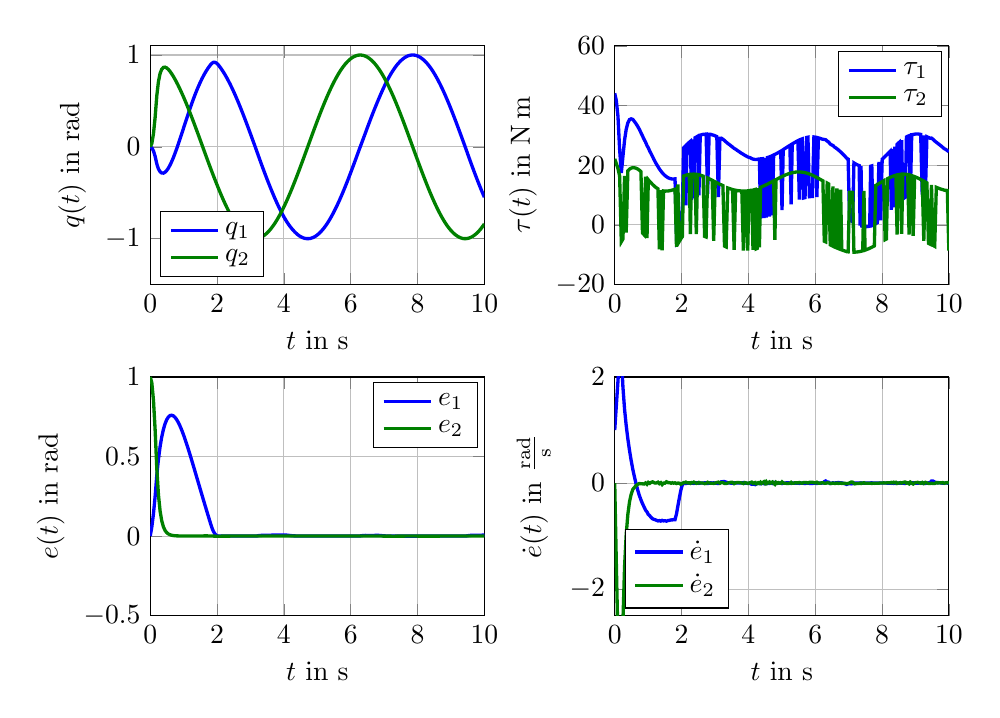
\begin{tikzpicture}

\begin{axis}[%
width=0.35\textwidth,
height=0.25\textwidth,
scale only axis,
xmin=0,
xmax=10,
xlabel={$t$ in $\mathrm{s}$},
xmajorgrids,
ymin=-1.5,
ymax=1.1,
ylabel={$q(t)$ in $\mathrm{rad}$},
ymajorgrids,
name=plot1,
legend style={at={(0.03,0.03)},anchor=south west,draw=black,fill=white,legend cell align=left}
]
\addplot [
color=blue,
solid,
line width=1.2pt
]
table[row sep=crcr]{
0 0\\
0.0469734754340576 -0.0106107250741021\\
0.0969734754340577 -0.0446434016324295\\
0.146973475434058 -0.104542833234935\\
0.196834763019643 -0.186450612199358\\
0.246281744490247 -0.241246395186037\\
0.294990561586982 -0.271527080329679\\
0.343483830242466 -0.285351339601509\\
0.393465620582656 -0.286445342405503\\
0.443465620582656 -0.276870997563999\\
0.493333043444229 -0.258106702825331\\
0.543111722236812 -0.231725008941364\\
0.592397706361066 -0.19915587239634\\
0.641390205310326 -0.161358886271839\\
0.689868062507002 -0.119483949732033\\
0.73755821980468 -0.0747046704405672\\
0.78435357881817 -0.0279565364970779\\
0.830923055342821 0.0207323872734872\\
0.87737039548458 0.0709169006000652\\
0.923357238492789 0.121710738637469\\
0.965651984464323 0.168941771023802\\
1.00565918085758 0.213832496582575\\
1.04857272474606 0.261885060925808\\
1.09016316293911 0.308148128383795\\
1.13142427668298 0.353449566233846\\
1.17088979783517 0.396045231880318\\
1.21371963442809 0.441258773412526\\
1.25245442405487 0.481103632118792\\
1.2935243492323 0.52210747694667\\
1.33632798421166 0.563366241102352\\
1.37818333758309 0.602110491962292\\
1.41900828196011 0.638293251917829\\
1.46036190067403 0.673221745725081\\
1.50269367055127 0.707152613483073\\
1.54827070360389 0.741634510653217\\
1.59536588042732 0.774967956465927\\
1.64158746569546 0.805260540481341\\
1.68758807576559 0.833061304014545\\
1.72497421042138 0.853903469742076\\
1.76363381703331 0.873914638435629\\
1.80480333204296 0.893509906711627\\
1.84835743986867 0.910798491269519\\
1.88971800809382 0.919559029549761\\
1.93552711087943 0.920286380464183\\
1.97674579039661 0.913435674114862\\
2.02347410586294 0.898197380569278\\
2.06201858285267 0.881035347791468\\
2.09562092555894 0.864807679186716\\
2.12850660206554 0.847935410606459\\
2.16409404693732 0.82862552597803\\
2.19781598669858 0.809344717747368\\
2.23146632030536 0.789187225362091\\
2.2645413685333 0.768482457307\\
2.29784617932889 0.746779535163222\\
2.33199346602012 0.723679537234785\\
2.36860428118823 0.697956456785037\\
2.40427700268403 0.672012489160047\\
2.44118704495532 0.644258473013346\\
2.47930153682729 0.614651732190218\\
2.51907943106166 0.582785007694171\\
2.55948076081918 0.549471928480821\\
2.60048716809277 0.514773196868659\\
2.64488784407351 0.476184423142734\\
2.69015293518711 0.43591919287162\\
2.73460247987575 0.395485504922927\\
2.77945688802513 0.353894374739592\\
2.82506852726477 0.310872615506429\\
2.87000375850878 0.267896391751469\\
2.91652325447558 0.222774975107346\\
2.96173455810371 0.178476841283079\\
3.00827778363793 0.13248493265419\\
3.05534489677939 0.0856170920017167\\
3.10181742839534 0.0392484624340703\\
3.14793231778836 -0.0068200878391915\\
3.19104956546572 -0.0504924482790744\\
3.23739828731297 -0.0983410574599269\\
3.28562191352634 -0.147479130821155\\
3.3340306556395 -0.195943498864883\\
3.38279414311744 -0.244025767905348\\
3.43087239701038 -0.290746680696088\\
3.47882325873143 -0.33657653742804\\
3.52616270326322 -0.381026127874559\\
3.57331315440706 -0.424330174804003\\
3.61876578448132 -0.465159200266349\\
3.6650495606391 -0.506009789437427\\
3.71175970768626 -0.54610732715313\\
3.75730941777774 -0.584139776627631\\
3.80382213207198 -0.621662677418229\\
3.85040608545862 -0.657846094394842\\
3.89530913722085 -0.691363279528875\\
3.93877298431134 -0.72228979862885\\
3.9800209614344 -0.750315007189463\\
4.01829630390428 -0.7751055082319\\
4.05391881380344 -0.797110144066712\\
4.09732165379995 -0.822650445449215\\
4.13802413074229 -0.844456329849003\\
4.17283320767611 -0.862073151274064\\
4.20742312572815 -0.878398960746137\\
4.2366861099218 -0.891458345108476\\
4.26581892385868 -0.903894027399933\\
4.29666903355405 -0.916407089345109\\
4.33031768950094 -0.929153859066701\\
4.36461617194131 -0.941211102257548\\
4.39800148219797 -0.951942454980701\\
4.43263907080445 -0.961996861808936\\
4.46633155284644 -0.970689924193912\\
4.49937467537644 -0.978152683189687\\
4.53262233583464 -0.984555666926487\\
4.56336976005034 -0.989535345344399\\
4.5956622364148 -0.993792304968749\\
4.62799968798673 -0.997012307558502\\
4.65900427046178 -0.999148813600103\\
4.69007565066579 -1.00031540420425\\
4.72228309597634 -1.00053706191303\\
4.75577557383643 -0.999667124309019\\
4.79237353312661 -0.997462496203021\\
4.8267035814252 -0.994164666507723\\
4.86316472304117 -0.989365776515535\\
4.89808240257891 -0.983525838585821\\
4.93296850414727 -0.976482152912806\\
4.96827376163078 -0.968140297323085\\
5.00623023032884 -0.957856673921125\\
5.042160294878 -0.946826358221026\\
5.07719796027609 -0.934861296913526\\
5.1180457927234 -0.919519876142656\\
5.15833493228003 -0.902884179527656\\
5.2002093812946 -0.884022463291917\\
5.2428334386473 -0.863243064979898\\
5.27844176694599 -0.844640827344177\\
5.3122009602999 -0.825997885520918\\
5.35617976736705 -0.80041062794795\\
5.39379749186081 -0.777226706051052\\
5.43818443708367 -0.748503182637018\\
5.48225314543699 -0.718539738483042\\
5.52499700314259 -0.688106809655772\\
5.5664056969738 -0.657447958938105\\
5.60926356081769 -0.624521103745526\\
5.65248375039042 -0.59016978092756\\
5.69548230803521 -0.554892004189553\\
5.73888261803292 -0.518249872988711\\
5.78243988952529 -0.48048616507276\\
5.82617219703852 -0.441653716843805\\
5.87068216869365 -0.401328390436902\\
5.91475341769844 -0.360533352330468\\
5.96061012841546 -0.31737651703821\\
6.00604328872926 -0.273951894813667\\
6.04923647039352 -0.232167290161864\\
6.09444957594157 -0.188000378527878\\
6.13918662666057 -0.14384013373747\\
6.18471330614499 -0.0986174351080816\\
6.22932356781612 -0.0542029300110703\\
6.27127884982597 -0.0125570347033341\\
6.3118083439689 0.0266055639493092\\
6.35825746664573 0.0716121385256866\\
6.40258366767117 0.11507859525579\\
6.45000192717153 0.1617042687384\\
6.49209827874995 0.203268717153082\\
6.53022712894764 0.240365614313684\\
6.57357362020017 0.282394362921283\\
6.61133559907904 0.318452916251459\\
6.64882884040464 0.353580713487388\\
6.68613419884582 0.387951533842686\\
6.72299736567756 0.421366405711286\\
6.75913910725831 0.453629295732726\\
6.79489325117898 0.485083695992687\\
6.82988001443984 0.515389910975073\\
6.86422480382322 0.544684955133719\\
6.89865864781635 0.573610555328723\\
6.93802754473797 0.6062390441646\\
6.98437977080357 0.643286065323934\\
7.0296506658098 0.677801780323951\\
7.07641004506731 0.711767182863955\\
7.12008872580689 0.742024718518282\\
7.15820012515548 0.767217356686576\\
7.18630971314135 0.78499627665324\\
7.2126843449465 0.801076930752054\\
7.2380393705171 0.816018000854643\\
7.26371060456435 0.830618655650969\\
7.2893917443135 0.844660485093352\\
7.31482709999231 0.858018471925045\\
7.34317918226088 0.872300836670488\\
7.37073545597436 0.885442319604021\\
7.39668972402114 0.897262919297274\\
7.42119046086587 0.907838167307666\\
7.45816523174438 0.922735755922529\\
7.49146555652101 0.935115158380981\\
7.53565891991457 0.949867860617044\\
7.57545879429014 0.961590091275039\\
7.60298807435246 0.968838311101847\\
7.6303902099379 0.975322110404041\\
7.65889154411081 0.981287173453885\\
7.69362477660863 0.987459650820552\\
7.73009410878359 0.992636942258681\\
7.76904702073196 0.996692760125465\\
7.81246961347454 0.999395284974475\\
7.85854049199615 1.00020582451029\\
7.90691924176834 0.998740030619935\\
7.95631260979146 0.994818178152816\\
8.00405769123183 0.988692039608689\\
8.05006073177866 0.9806488424493\\
8.09162987737557 0.971608561324162\\
8.13053186938092 0.961665240995618\\
8.16732497740632 0.950944757344842\\
8.20550921399351 0.938442042853908\\
8.24157620470039 0.925409012156836\\
8.2773967042953 0.911269710127407\\
8.3123580457709 0.896370668305747\\
8.34653886600855 0.880727918218006\\
8.38075412750439 0.864034971252376\\
8.41502838990159 0.846321783438054\\
8.44918953137318 0.82766482814787\\
8.48359435312928 0.807890075089497\\
8.51799030354735 0.787189032072225\\
8.55193838242961 0.765813815012933\\
8.58642822714714 0.74321889068349\\
8.62108100696298 0.719612650633398\\
8.65758127689534 0.693817144065004\\
8.69292992790833 0.667968499456422\\
8.72985722511527 0.640064289347423\\
8.7682038719411 0.610134147059435\\
8.80830540240105 0.577874330425383\\
8.84649288136568 0.546300093185691\\
8.88765267149246 0.511360127149243\\
8.93063424388249 0.473940469404649\\
8.97522358457664 0.434221073828579\\
9.01964503919037 0.393783562118144\\
9.06358407277127 0.353030460578082\\
9.10970586861994 0.309532327310428\\
9.1560683293571 0.265127294194542\\
9.20226441880243 0.220289529376359\\
9.24890202733427 0.174556912432188\\
9.29573327029446 0.128221449552489\\
9.34221764285631 0.0818839927862466\\
9.38877182715508 0.0354668375419204\\
9.4355642264296 -0.0114630563805996\\
9.47911101447991 -0.0559222397005817\\
9.52698835078501 -0.105256153477164\\
9.57537892390731 -0.154344400166673\\
9.6239656011718 -0.202879084889413\\
9.67240650004054 -0.250415410111976\\
9.72061971572214 -0.297126263138888\\
9.7684590483958 -0.34271059815664\\
9.81619213858135 -0.387347648107788\\
9.86228434470425 -0.4294254983115\\
9.90728536715671 -0.469854387577216\\
9.95349508642141 -0.510416099860577\\
9.99878892568466 -0.549149951589104\\
};
\addlegendentry{$q_1$};

\addplot [
color=green!50!black,
solid,
line width=1.2pt
]
table[row sep=crcr]{
0 0\\
0.0469734754340576 0.0342188565338217\\
0.0969734754340577 0.142100865717834\\
0.146973475434058 0.323646811931532\\
0.196834763019643 0.557671246247101\\
0.246281744490247 0.71233952859036\\
0.294990561586982 0.798894123073982\\
0.343483830242466 0.844546930575684\\
0.393465620582656 0.864660959023474\\
0.443465620582656 0.867701037142677\\
0.493333043444229 0.858949717260218\\
0.543111722236812 0.842657755262737\\
0.592397706361066 0.82121083364388\\
0.641390205310326 0.79592516166325\\
0.689868062507002 0.767835461531775\\
0.73755821980468 0.737757760315889\\
0.78435357881817 0.706182667333974\\
0.830923055342821 0.672962665908241\\
0.87737039548458 0.638178877457338\\
0.923357238492789 0.602239193355678\\
0.965651984464323 0.568132616481099\\
1.00565918085758 0.534849613457719\\
1.04857272474606 0.498211557878674\\
1.09016316293911 0.461710737520415\\
1.13142427668298 0.424749217918934\\
1.17088979783517 0.388715910358624\\
1.21371963442809 0.348935495055931\\
1.25245442405487 0.312374061961355\\
1.2935243492323 0.273104970299522\\
1.33632798421166 0.231644235698086\\
1.37818333758309 0.190712023670821\\
1.41900828196011 0.150458880546913\\
1.46036190067403 0.109493167176546\\
1.50269367055127 0.0673456138065222\\
1.54827070360389 0.0216474125932925\\
1.59536588042732 -0.0257631415611889\\
1.64158746569546 -0.0720518689628674\\
1.68758807576559 -0.117872650161437\\
1.72497421042138 -0.154767125543489\\
1.76363381703331 -0.192765693313647\\
1.80480333204296 -0.232889268026855\\
1.84835743986867 -0.27453308207634\\
1.88971800809382 -0.313604754973009\\
1.93552711087943 -0.356361589885842\\
1.97674579039661 -0.394368997189517\\
2.02347410586294 -0.436685403705286\\
2.06201858285267 -0.471102925437583\\
2.09562092555894 -0.500626054578118\\
2.12850660206554 -0.528888359545692\\
2.16409404693732 -0.55881501957778\\
2.19781598669858 -0.586498468537088\\
2.23146632030536 -0.613460385962891\\
2.2645413685333 -0.63925648625786\\
2.29784617932889 -0.66451715801206\\
2.33199346602012 -0.689691496745736\\
2.36860428118823 -0.715780138770888\\
2.40427700268403 -0.740432585757495\\
2.44118704495532 -0.764912036217583\\
2.47930153682729 -0.789022386518157\\
2.51907943106166 -0.812929465992285\\
2.55948076081918 -0.835928471731159\\
2.60048716809277 -0.85784195583171\\
2.64488784407351 -0.879789825862334\\
2.69015293518711 -0.900395879499397\\
2.73460247987575 -0.918848026759428\\
2.77945688802513 -0.935638763443814\\
2.82506852726477 -0.950779085965297\\
2.87000375850878 -0.963821671500058\\
2.91652325447558 -0.975215062705734\\
2.96173455810371 -0.984345253170143\\
3.00827778363793 -0.991667775568245\\
3.05534489677939 -0.996815679192085\\
3.10181742839534 -0.999754090932573\\
3.14793231778836 -1.00045813196612\\
3.19104956546572 -0.999237506980856\\
3.23739828731297 -0.995898680481192\\
3.28562191352634 -0.990098832350868\\
3.3340306556395 -0.982010541230771\\
3.38279414311744 -0.971548976192957\\
3.43087239701038 -0.958982706728997\\
3.47882325873143 -0.944215531190939\\
3.52616270326322 -0.927543044181091\\
3.57331315440706 -0.908805153862236\\
3.61876578448132 -0.888842597191353\\
3.6650495606391 -0.86661762702553\\
3.71175970768626 -0.8423712574993\\
3.75730941777774 -0.816864595480185\\
3.80382213207198 -0.789109398024065\\
3.85040608545862 -0.759608268623264\\
3.89530913722085 -0.729627865533203\\
3.93877298431134 -0.699204892732255\\
3.9800209614344 -0.669113568952685\\
4.01829630390428 -0.640206587494583\\
4.05391881380344 -0.612437518990484\\
4.09732165379995 -0.577528510067905\\
4.13802413074229 -0.543813743831356\\
4.17283320767611 -0.514259248817066\\
4.20742312572815 -0.484274994437546\\
4.2366861099218 -0.458407624100032\\
4.26581892385868 -0.43229252415442\\
4.29666903355405 -0.404289176020452\\
4.33031768950094 -0.373378212441985\\
4.36461617194131 -0.341358378332848\\
4.39800148219797 -0.309820647450548\\
4.43263907080445 -0.276730006392296\\
4.46633155284644 -0.244206033448349\\
4.49937467537644 -0.212099312624214\\
4.53262233583464 -0.179566244423414\\
4.56336976005034 -0.149294529161421\\
4.5956622364148 -0.117279430368744\\
4.62799968798673 -0.085124196211423\\
4.65900427046178 -0.0541905314719828\\
4.69007565066579 -0.0231265951515448\\
4.72228309597634 0.00907668916234206\\
4.75577557383643 0.0424455079948274\\
4.79237353312661 0.0788619783824668\\
4.8267035814252 0.113038549599407\\
4.86316472304117 0.14917658676219\\
4.89808240257891 0.183634459306001\\
4.93296850414727 0.217810987223586\\
4.96827376163078 0.252124952869202\\
5.00623023032884 0.288652651093256\\
5.042160294878 0.322875396675023\\
5.07719796027609 0.35582582149283\\
5.1180457927234 0.393641976814365\\
5.15833493228003 0.430313921837654\\
5.2002093812946 0.4676924404124\\
5.2428334386473 0.504911906177537\\
5.27844176694599 0.535368621080486\\
5.3122009602999 0.563566477255201\\
5.35617976736705 0.599303704130154\\
5.39379749186081 0.628986965724496\\
5.43818443708367 0.662803952314569\\
5.48225314543699 0.695095909801872\\
5.52499700314259 0.725155908128849\\
5.5664056969738 0.753010994331187\\
5.60926356081769 0.780482735127467\\
5.65248375039042 0.806824118064462\\
5.69548230803521 0.831527679129845\\
5.73888261803292 0.854827483495829\\
5.78243988952529 0.876574013475727\\
5.82617219703852 0.896776738616718\\
5.87068216869365 0.915595347273591\\
5.91475341769844 0.93236382880894\\
5.96061012841546 0.947920109978086\\
6.00604328872926 0.961436404815956\\
6.04923647039352 0.972370218709546\\
6.09444957594157 0.9818678119846\\
6.13918662666057 0.989364835821041\\
6.18471330614499 0.994906490553342\\
6.22932356781612 0.99829563778227\\
6.27127884982597 0.999595206563599\\
6.3118083439689 0.999186745776812\\
6.35825746664573 0.996739368199776\\
6.40258366767117 0.992393154051858\\
6.45000192717153 0.985620497916632\\
6.49209827874995 0.977826716697484\\
6.53022712894764 0.969248325777082\\
6.57357362020017 0.95776864270646\\
6.61133559907904 0.946286236846741\\
6.64882884040464 0.933562552909178\\
6.68613419884582 0.919575861317666\\
6.72299736567756 0.904512621821794\\
6.75913910725831 0.888550379756203\\
6.79489325117898 0.871591576208581\\
6.82988001443984 0.853933600000823\\
6.86422480382322 0.835570186367283\\
6.89865864781635 0.816176787933722\\
6.93802754473797 0.792960402571567\\
6.98437977080357 0.764192762544144\\
7.0296506658098 0.734398988986487\\
7.07641004506731 0.701942261305558\\
7.12008872580689 0.670074633152596\\
7.15820012515548 0.641163585637724\\
7.18630971314135 0.619409005847648\\
7.2126843449465 0.598607915852788\\
7.2380393705171 0.578193790885267\\
7.26371060456435 0.557101903224986\\
7.2893917443135 0.535595149156305\\
7.31482709999231 0.513926932722117\\
7.34317918226088 0.489227735797088\\
7.37073545597436 0.465056373608994\\
7.39668972402114 0.441766256424218\\
7.42119046086587 0.419575305366895\\
7.45816523174438 0.38576424763816\\
7.49146555652101 0.354716427475832\\
7.53565891991457 0.313139784039526\\
7.57545879429014 0.275064085393929\\
7.60298807435246 0.248354486265438\\
7.6303902099379 0.221569436372008\\
7.65889154411081 0.193548485685236\\
7.69362477660863 0.159250317606561\\
7.73009410878359 0.123098089901063\\
7.76904702073196 0.0843313298488016\\
7.81246961347454 0.0410519667661062\\
7.85854049199615 -0.00493077774187867\\
7.90691924176834 -0.0531816425089685\\
7.95631260979146 -0.102319184481481\\
8.00405769123183 -0.149550886086703\\
8.05006073177866 -0.194741471422848\\
8.09162987737557 -0.235244494147865\\
8.13053186938092 -0.272844948795241\\
8.16732497740632 -0.308035007940472\\
8.20550921399351 -0.344090093278819\\
8.24157620470039 -0.37772458712089\\
8.2773967042953 -0.410619144642997\\
8.3123580457709 -0.442265519904687\\
8.34653886600855 -0.472660624592972\\
8.38075412750439 -0.502512127489076\\
8.41502838990159 -0.531897896493251\\
8.44918953137318 -0.560528523349962\\
8.48359435312928 -0.588681339452663\\
8.51799030354735 -0.61617443975226\\
8.55193838242961 -0.642542892525056\\
8.58642822714714 -0.66862458632722\\
8.62108100696298 -0.694007177985514\\
8.65758127689534 -0.719866817757749\\
8.69292992790833 -0.744168380519841\\
8.72985722511527 -0.768488984528679\\
8.7682038719411 -0.792562360354302\\
8.80830540240105 -0.816448382146398\\
8.84649288136568 -0.837983886243839\\
8.88765267149246 -0.85984085764107\\
8.93063424388249 -0.880964078818047\\
8.97522358457664 -0.901231890724086\\
9.01964503919037 -0.919617250600765\\
9.06358407277127 -0.936020148479138\\
9.10970586861994 -0.951304324780506\\
9.1560683293571 -0.964661538471335\\
9.20226441880243 -0.975895263685343\\
9.24890202733427 -0.985157869799519\\
9.29573327029446 -0.992257180901173\\
9.34221764285631 -0.997160710498022\\
9.38877182715508 -0.999928727462929\\
9.4355642264296 -1.00046132399096\\
9.47911101447991 -0.999031750337452\\
9.52698835078501 -0.995270531254105\\
9.57537892390731 -0.989167850786337\\
9.6239656011718 -0.980720223718716\\
9.67240650004054 -0.969993397640145\\
9.72061971572214 -0.95706872680031\\
9.7684590483958 -0.942082466575241\\
9.81619213858135 -0.924957901744395\\
9.86228434470425 -0.906302333490341\\
9.90728536715671 -0.886340652212119\\
9.95349508642141 -0.86394465646726\\
9.99878892568466 -0.840207741189448\\
};
\addlegendentry{$q_2$};

\end{axis}

\begin{axis}[%
width=0.35\textwidth,
height=0.25\textwidth,
scale only axis,
xmin=0,
xmax=10,
xlabel={$t$ in $\mathrm{s}$},
xmajorgrids,
ymin=-0.5,
ymax=1,
ylabel={$e(t)$ in $\mathrm{rad}$},
ymajorgrids,
name=plot3,
at=(plot1.below south west),
anchor=above north west,
legend style={draw=black,fill=white,legend cell align=left}
]
\addplot [
color=blue,
solid,
line width=1.2pt
]
table[row sep=crcr]{
0 0\\
0.0469734754340576 0.0575669278604004\\
0.0969734754340577 0.141464961097904\\
0.146973475434058 0.250987745904615\\
0.196834763019643 0.382016809993062\\
0.246281744490247 0.485045988561101\\
0.294990561586982 0.562257899746576\\
0.343483830242466 0.622120798536923\\
0.393465620582656 0.669836851858062\\
0.443465620582656 0.705943424463742\\
0.493333043444229 0.731670825170329\\
0.543111722236812 0.748527458323916\\
0.592397706361066 0.757507645894243\\
0.641390205310326 0.759668827966048\\
0.689868062507002 0.755919370148332\\
0.73755821980468 0.747187395809771\\
0.78435357881817 0.734324299196221\\
0.830923055342821 0.717821617053847\\
0.87737039548458 0.69814385994529\\
0.923357238492789 0.675920276699097\\
0.965651984464323 0.653478221596938\\
1.00565918085758 0.630682665794128\\
1.04857272474606 0.604827110545463\\
1.09016316293911 0.578554234735158\\
1.13142427668298 0.551569387226643\\
1.17088979783517 0.525052157436491\\
1.21371963442809 0.495663855797006\\
1.25245442405487 0.468652062817118\\
1.2935243492323 0.439698288702777\\
1.33632798421166 0.40927175547939\\
1.37818333758309 0.379396905041966\\
1.41900828196011 0.350209043477975\\
1.46036190067403 0.320686567879023\\
1.50269367055127 0.290529296767252\\
1.54827070360389 0.258111798223969\\
1.59536588042732 0.224730227234626\\
1.64158746569546 0.192234813086418\\
1.68758807576559 0.160126288569672\\
1.72497421042138 0.134234645538948\\
1.76363381703331 0.107549758902143\\
1.80480333204296 0.0792351669773688\\
1.84835743986867 0.0509280882924702\\
1.88971800809382 0.0300150396002306\\
1.93552711087943 0.0139334432790756\\
1.97674579039661 0.0052922023590547\\
2.02347410586294 0.00108175324642279\\
2.06201858285267 0.000721626556310584\\
2.09562092555894 0.000604162505166705\\
2.12850660206554 0.000533748507202003\\
2.16409404693732 0.000475915277379113\\
2.19781598669858 0.000435051089987093\\
2.23146632030536 0.00039404454371661\\
2.2645413685333 0.000374296460486145\\
2.29784617932889 0.000358985329783179\\
2.33199346602012 0.000331219421556672\\
2.36860428118823 0.000321054710816449\\
2.40427700268403 0.00029068807513144\\
2.44118704495532 0.000269387818190636\\
2.47930153682729 0.000273473452866213\\
2.51907943106166 0.000293773370709571\\
2.55948076081918 0.000317304303280697\\
2.60048716809277 0.000310664936942318\\
2.64488784407351 0.000346716122087254\\
2.69015293518711 0.000342280259825634\\
2.73460247987575 0.000361647358904094\\
2.77945688802513 0.000377909775770513\\
2.82506852726477 0.000392629105233022\\
2.87000375850878 0.000366038436126204\\
2.91652325447558 0.000399036334645664\\
2.96173455810371 0.00041311847966688\\
3.00827778363793 0.000435390439945754\\
3.05534489677939 0.000523776391806827\\
3.10181742839534 0.000516275734570491\\
3.14793231778836 0.000480466107144194\\
3.19104956546572 0.00105569575761331\\
3.23739828731297 0.00268191866112061\\
3.28562191352634 0.00394732206584406\\
3.3340306556395 0.00469103919663869\\
3.38279414311744 0.00515626092542454\\
3.43087239701038 0.0054847111592487\\
3.47882325873143 0.00570158072008314\\
3.52616270326322 0.00586550311600109\\
3.57331315440706 0.00589611382543487\\
3.61876578448132 0.00588928501300012\\
3.6650495606391 0.00613265623610759\\
3.71175970768626 0.00633464294286656\\
3.75730941777774 0.00659596864243317\\
3.80382213207198 0.00678607999346825\\
3.85040608545862 0.00691263006874288\\
3.89530913722085 0.00700992353856866\\
3.93877298431134 0.00690103931106167\\
3.9800209614344 0.0067218525886692\\
4.01829630390428 0.00647108589335854\\
4.05391881380344 0.00618087073035922\\
4.09732165379995 0.005915845046366\\
4.13802413074229 0.00491877986157807\\
4.17283320767611 0.0041361613079669\\
4.20742312572815 0.00320796705890536\\
4.2366861099218 0.00248729281215465\\
4.26581892385868 0.00196031743266056\\
4.29666903355405 0.00158128130103541\\
4.33031768950094 0.00125949922684854\\
4.36461617194131 0.00107702076288807\\
4.39800148219797 0.000956491277753435\\
4.43263907080445 0.000872339653442133\\
4.46633155284644 0.000809627291814663\\
4.49937467537644 0.000754572442153045\\
4.53262233583464 0.000670223399572678\\
4.56336976005034 0.000618177113878904\\
4.5956622364148 0.000597139683115699\\
4.62799968798673 0.000570971207772719\\
4.65900427046178 0.000573438838803897\\
4.69007565066579 0.000564336217274475\\
4.72228309597634 0.000586008275408889\\
4.75577557383643 0.000608174921600035\\
4.79237353312661 0.000659555556426272\\
4.8267035814252 0.000691468273221307\\
4.86316472304117 0.000710921611397852\\
4.89808240257891 0.000717376869008191\\
4.93296850414727 0.000711336703892229\\
4.96827376163078 0.000700562374067348\\
5.00623023032884 0.000718279207790329\\
5.042160294878 0.000709935486764679\\
5.07719796027609 0.000669368298744977\\
5.1180457927234 0.00067647359327272\\
5.15833493228003 0.000681110357791836\\
5.2002093812946 0.00066592556378231\\
5.2428334386473 0.000660768149073232\\
5.27844176694599 0.000616373446375551\\
5.3122009602999 0.000556121074587579\\
5.35617976736705 0.000584468424343343\\
5.39379749186081 0.000540420512624706\\
5.43818443708367 0.000531492952421386\\
5.48225314543699 0.000534516001793661\\
5.52499700314259 0.000499676904585744\\
5.5664056969738 0.000487809485875124\\
5.60926356081769 0.000465950227493295\\
5.65248375039042 0.000458290830698371\\
5.69548230803521 0.000441118788179318\\
5.73888261803292 0.000428198015146153\\
5.78243988952529 0.000406594190193954\\
5.82617219703852 0.000383996359104355\\
5.87068216869365 0.000424633205008462\\
5.91475341769844 0.000380356684762218\\
5.96061012841546 0.000366551263718706\\
6.00604328872926 0.000344049865082019\\
6.04923647039352 0.000346704401047226\\
6.09444957594157 0.000383151432932577\\
6.13918662666057 0.00033858783845836\\
6.18471330614499 0.000304499749303466\\
6.22932356781612 0.000367229801908987\\
6.27127884982597 0.000650858665018178\\
6.3118083439689 0.00201356462825578\\
6.35825746664573 0.00338952516467535\\
6.40258366767117 0.00403627750341508\\
6.45000192717153 0.00433973754606309\\
6.49209827874995 0.00412791233171966\\
6.53022712894764 0.00417105099377821\\
6.57357362020017 0.00392993918902124\\
6.61133559907904 0.00383965661148594\\
6.64882884040464 0.00396964671205563\\
6.68613419884582 0.00418122043640684\\
6.72299736567756 0.00440301144664601\\
6.75913910725831 0.00455715075722496\\
6.79489325117898 0.00458343688627338\\
6.82988001443984 0.00447662480721067\\
6.86422480382322 0.00420818553417701\\
6.89865864781635 0.00373451437151395\\
6.93802754473797 0.00279507840720272\\
6.98437977080357 0.00184473830071752\\
7.0296506658098 0.00124646925184702\\
7.07641004506731 0.000852108821007502\\
7.12008872580689 0.000547981682070264\\
7.15820012515548 0.000335643741174452\\
7.18630971314135 0.000268968323821062\\
7.2126843449465 0.000243417308932958\\
7.2380393705171 0.000211436604270698\\
7.26371060456435 0.00017120273200133\\
7.2893917443135 0.000147623859781842\\
7.31482709999231 0.000124587345930571\\
7.34317918226088 5.16513563776355e-05\\
7.37073545597436 4.89149808946543e-05\\
7.39668972402114 -1.14575028016262e-05\\
7.42119046086587 -3.95154089697369e-05\\
7.45816523174438 -5.36573824236886e-05\\
7.49146555652101 -0.000107645437697812\\
7.53565891991457 -0.000106159948701667\\
7.57545879429014 -0.000127480028199733\\
7.60298807435246 -0.000172178171106263\\
7.6303902099379 -0.00021470821766334\\
7.65889154411081 -0.000256964286185379\\
7.69362477660863 -0.000289284179566751\\
7.73009410878359 -0.000301191529690992\\
7.76904702073196 -0.000297536568978907\\
7.81246961347454 -0.000256785171944607\\
7.85854049199615 -0.000216216085526466\\
7.90691924176834 -0.000140898585322846\\
7.95631260979146 -4.9425094585609e-05\\
8.00405769123183 6.76696129896515e-05\\
8.05006073177866 0.000189162907017315\\
8.09162987737557 0.000285745615913879\\
8.13053186938092 0.00033783866081849\\
8.16732497740632 0.000363576091167328\\
8.20550921399351 0.000405770344715894\\
8.24157620470039 0.000411887359735186\\
8.2773967042953 0.000421377731998684\\
8.3123580457709 0.000401436798327381\\
8.34653886600855 0.000398557128608479\\
8.38075412750439 0.000399214719686625\\
8.41502838990159 0.000376841208020395\\
8.44918953137318 0.000367124483714676\\
8.48359435312928 0.000365537100164626\\
8.51799030354735 0.000339075783922671\\
8.55193838242961 0.000343073579916031\\
8.58642822714714 0.000321724354912289\\
8.62108100696298 0.000314224705068589\\
8.65758127689534 0.000302831325278752\\
8.69292992790833 0.000277102791416572\\
8.72985722511527 0.000260268897790739\\
8.7682038719411 0.000272668964670042\\
8.80830540240105 0.000286312453163129\\
8.84649288136568 0.000288571426899864\\
8.88765267149246 0.000308079157677388\\
8.93063424388249 0.00033750546055672\\
8.97522358457664 0.00034315644209465\\
9.01964503919037 0.000357363313387316\\
9.06358407277127 0.000360877356544831\\
9.10970586861994 0.000352688066645956\\
9.1560683293571 0.000360301088275061\\
9.20226441880243 0.000392360940560083\\
9.24890202733427 0.000413713157927598\\
9.29573327029446 0.000465385536406265\\
9.34221764285631 0.000582565729682696\\
9.38877182715508 0.000531516601418022\\
9.4355642264296 0.00067699987119608\\
9.47911101447991 0.00161591463792245\\
9.52698835078501 0.00322363523298905\\
9.57537892390731 0.00431207974443987\\
9.6239656011718 0.00500598605129776\\
9.67240650004054 0.00530988213962716\\
9.72061971572214 0.00558112317030646\\
9.7684590483958 0.00575541075947911\\
9.81619213858135 0.00585162771919279\\
9.86228434470425 0.00574345846063912\\
9.90728536715671 0.00585260925341291\\
9.95349508642141 0.00599004740501241\\
9.99878892568466 0.00614541738703345\\
};
\addlegendentry{$e_1$};

\addplot [
color=green!50!black,
solid,
line width=1.2pt
]
table[row sep=crcr]{
0 1\\
0.0469734754340576 0.964678092615535\\
0.0969734754340577 0.853200890345458\\
0.146973475434058 0.665572014998672\\
0.196834763019643 0.423019256552082\\
0.246281744490247 0.2574861043304\\
0.294990561586982 0.157910763327201\\
0.343483830242466 0.0970402037503694\\
0.393465620582656 0.058924960357981\\
0.443465620582656 0.035569051188805\\
0.493333043444229 0.0218096267308703\\
0.543111722236812 0.0134469277709417\\
0.592397706361066 0.0083934678346903\\
0.641390205310326 0.00533959712118104\\
0.689868062507002 0.00349452987237642\\
0.73755821980468 0.00235505816519144\\
0.78435357881817 0.00166236077557425\\
0.830923055342821 0.00123165525744529\\
0.87737039548458 0.000996799950212401\\
0.923357238492789 0.000906529810090762\\
0.965651984464323 0.000748175722066313\\
1.00565918085758 0.000682029413036078\\
1.04857272474606 0.000597034492742121\\
1.09016316293911 0.000629958546093379\\
1.13142427668298 0.000622024500296359\\
1.17088979783517 0.000616337719747673\\
1.21371963442809 0.00060132256861839\\
1.25245442405487 0.000618142313459469\\
1.2935243492323 0.000627872383780037\\
1.33632798421166 0.000681672468555189\\
1.37818333758309 0.000712190121280709\\
1.41900828196011 0.000746979118729979\\
1.46036190067403 0.000716923779982351\\
1.50269367055127 0.000704411610547045\\
1.54827070360389 0.000876305715279132\\
1.59536588042732 0.0011960598090877\\
1.64158746569546 0.00131984219470052\\
1.68758807576559 0.00134623282714126\\
1.72497421042138 0.00119933878836698\\
1.76363381703331 0.00112113492910679\\
1.80480333204296 0.00101209878893682\\
1.84835743986867 0.000522158637151937\\
1.88971800809382 6.19553460261546e-05\\
1.93552711087943 -0.000336210675242976\\
1.97674579039661 -0.000522239722278772\\
2.02347410586294 -0.000689766467510289\\
2.06201858285267 -0.000601047610186867\\
2.09562092555894 -0.000435163497540692\\
2.12850660206554 -0.000356466629262142\\
2.16409404693732 -0.000283182984348929\\
2.19781598669858 -0.000235479672592631\\
2.23146632030536 -0.000185618027953693\\
2.2645413685333 -0.000164573909947507\\
2.29784617932889 -0.000151203801199484\\
2.33199346602012 -9.71841166798049e-05\\
2.36860428118823 -4.70170000829162e-05\\
2.40427700268403 0.000156665657777166\\
2.44118704495532 0.000331212097645195\\
2.47930153682729 0.000436949507802931\\
2.51907943106166 0.00051384879140115\\
2.55948076081918 0.000625054094986588\\
2.60048716809277 0.000702168336445208\\
2.64488784407351 0.000632232872901928\\
2.69015293518711 0.00057593803267153\\
2.73460247987575 0.000531615041568734\\
2.77945688802513 0.000496448913953174\\
2.82506852726477 0.000456010639415028\\
2.87000375850878 0.000475799785311315\\
2.91652325447558 0.000436441368104057\\
2.96173455810371 0.000476165183289745\\
3.00827778363793 0.000541049206499888\\
3.05534489677939 0.000532711962187071\\
3.10181742839534 0.000545020918504724\\
3.14793231778836 0.000478227569893241\\
3.19104956546572 0.000460250781991745\\
3.23739828731297 0.000484530911139536\\
3.28562191352634 0.000453128133733327\\
3.3340306556395 0.000469662473881582\\
3.38279414311744 0.000497299589096833\\
3.43087239701038 0.000533120816434307\\
3.47882325873143 0.000540924653544272\\
3.52616270326322 0.000583225402106313\\
3.57331315440706 0.000557975714687964\\
3.61876578448132 0.000545830934049585\\
3.6650495606391 0.00052129768194531\\
3.71175970768626 0.000560441828434621\\
3.75730941777774 0.000504901559694182\\
3.80382213207198 0.000486059579564713\\
3.85040608545862 0.000473481500172124\\
3.89530913722085 0.000477343250729234\\
3.93877298431134 0.000478248727780239\\
3.9800209614344 0.000481218231573655\\
4.01829630390428 0.00051828464991166\\
4.05391881380344 0.000529940528157469\\
4.09732165379995 0.000514998523505117\\
4.13802413074229 0.000512076098674985\\
4.17283320767611 0.000504325485023327\\
4.20742312572815 0.000497437528634237\\
4.2366861099218 0.000444232354391727\\
4.26581892385868 0.000418025226001373\\
4.29666903355405 0.00044051508852766\\
4.33031768950094 0.000535005480411355\\
4.36461617194131 0.000553582574055689\\
4.39800148219797 0.000586598807813865\\
4.43263907080445 0.000614717226023187\\
4.46633155284644 0.000623994535175032\\
4.49937467537644 0.000692280794260036\\
4.53262233583464 0.000766261157625348\\
4.56336976005034 0.00082623497397788\\
4.5956622364148 0.000817575440856949\\
4.62799968798673 0.00083503195187079\\
4.65900427046178 0.000831175025982678\\
4.69007565066579 0.000815116964072375\\
4.72228309597634 0.000817265001790286\\
4.75577557383643 0.000927474942784251\\
4.79237353312661 0.00103731772395846\\
4.8267035814252 0.00102724014366178\\
4.86316472304117 0.00102853257293828\\
4.89808240257891 0.00099361975521059\\
4.93296850414727 0.00098415494138604\\
4.96827376163078 0.000976527256407345\\
5.00623023032884 0.000978309554222123\\
5.042160294878 0.000951277075804502\\
5.07719796027609 0.000945030050560292\\
5.1180457927234 0.000980376317679332\\
5.15833493228003 0.000997592013386395\\
5.2002093812946 0.00100919949614819\\
5.2428334386473 0.00100486681389045\\
5.27844176694599 0.00093606957820791\\
5.3122009602999 0.00092080648795656\\
5.35617976736705 0.000928013243825743\\
5.39379749186081 0.000900654297140369\\
5.43818443708367 0.000926679365459537\\
5.48225314543699 0.00094180504528607\\
5.52499700314259 0.000927028586849232\\
5.5664056969738 0.000914308355825399\\
5.60926356081769 0.000897559842648832\\
5.65248375039042 0.000789872928598334\\
5.69548230803521 0.000688768483174118\\
5.73888261803292 0.000661097916905495\\
5.78243988952529 0.000650932374088753\\
5.82617219703852 0.000597783967556387\\
5.87068216869365 0.000524829033727081\\
5.91475341769844 0.000529423244811755\\
5.96061012841546 0.00050209642561061\\
6.00604328872926 0.0004049267884777\\
6.04923647039352 0.000388341272072323\\
6.09444957594157 0.000374406664753191\\
6.13918662666057 0.000285257052493049\\
6.18471330614499 0.000249058464569685\\
6.22932356781612 0.000254169379590774\\
6.27127884982597 0.000333912410413806\\
6.3118083439689 0.000403643072270476\\
6.35825746664573 0.000444040428585035\\
6.40258366767117 0.000487325707694164\\
6.45000192717153 0.000497845882429848\\
6.49209827874995 0.000430221983936163\\
6.53022712894764 0.000391720487667668\\
6.57357362020017 0.000364121591394317\\
6.61133559907904 0.000353872950738521\\
6.64882884040464 0.000331306114024099\\
6.68613419884582 0.000332777092416525\\
6.72299736567756 0.000319077121713418\\
6.75913910725831 0.000305727976038894\\
6.79489325117898 0.000317879513799579\\
6.82988001443984 0.000313896321951335\\
6.86422480382322 0.000322342686382315\\
6.89865864781635 0.000323469563376921\\
6.93802754473797 0.00018361811017209\\
6.98437977080357 -0.000120615286693715\\
7.0296506658098 -0.000305347311227333\\
7.07641004506731 -0.000391304411889393\\
7.12008872580689 -0.000309163068359375\\
7.15820012515548 -0.000178100985881668\\
7.18630971314135 -0.000249498910125601\\
7.2126843449465 -0.000372427283764187\\
7.2380393705171 -0.000465909071082238\\
7.26371060456435 -0.000515691387139361\\
7.2893917443135 -0.000525752678585567\\
7.31482709999231 -0.000516288281381727\\
7.34317918226088 -0.000350310839321299\\
7.37073545597436 -0.000400292756411513\\
7.39668972402114 -0.000246365244123081\\
7.42119046086587 -0.000169049320434433\\
7.45816523174438 -0.000202650699840434\\
7.49146555652101 -8.85228495646762e-05\\
7.53565891991457 -0.000165804380547196\\
7.57545879429014 -0.000128370772475961\\
7.60298807435246 1.20229764581092e-05\\
7.6303902099379 0.000163633334189089\\
7.65889154411081 0.000306430941554581\\
7.69362477660863 0.00042017818368581\\
7.73009410878359 0.000472771652665821\\
7.76904702073196 0.00050120208217673\\
7.81246961347454 0.000448132177752504\\
7.85854049199615 0.000371935511461281\\
7.90691924176834 0.000268756557442212\\
7.95631260979146 0.000166710507649145\\
8.00405769123183 3.7550829068117e-05\\
8.05006073177866 -8.35969042080331e-05\\
8.09162987737557 -0.000173126555154196\\
8.13053186938092 -0.00019364688590312\\
8.16732497740632 -0.000205895794256727\\
8.20550921399351 -0.000242280529049677\\
8.24157620470039 -0.000237926917641962\\
8.2773967042953 -0.000257187502983314\\
8.3123580457709 -0.000227182303165652\\
8.34653886600855 -0.000220052156726491\\
8.38075412750439 -0.000233870130812774\\
8.41502838990159 -0.00017487956510609\\
8.44918953137318 -0.000152388953216787\\
8.48359435312928 -0.0001504407391969\\
8.51799030354735 -0.000104295347788996\\
8.55193838242961 -0.000110686054978548\\
8.58642822714714 -6.61895836743254e-05\\
8.62108100696298 -4.27439692344267e-05\\
8.65758127689534 7.48444033327189e-06\\
8.69292992790833 0.000227646941941662\\
8.72985722511527 0.000384525416462167\\
8.7682038719411 0.000474285105522831\\
8.80830540240105 0.00052542559580171\\
8.84649288136568 0.000582649251066991\\
8.88765267149246 0.000657730098019282\\
8.93063424388249 0.000588930056021009\\
8.97522358457664 0.000591046786138638\\
9.01964503919037 0.000567235150040535\\
9.06358407277127 0.000544567679310881\\
9.10970586861994 0.000530283672551479\\
9.1560683293571 0.000547262697478179\\
9.20226441880243 0.00054942589950846\\
9.24890202733427 0.000584215784440123\\
9.29573327029446 0.000571898931735482\\
9.34221764285631 0.00056687812369971\\
9.38877182715508 0.000576878263173985\\
9.4355642264296 0.000519495190416164\\
9.47911101447991 0.000507427620078604\\
9.52698835078501 0.000489467290404888\\
9.57537892390731 0.000486758204547688\\
9.6239656011718 0.000492578344336359\\
9.67240650004054 0.000496992202045354\\
9.72061971572214 0.000511655130929545\\
9.7684590483958 0.000561780830023562\\
9.81619213858135 0.000587420591051324\\
9.86228434470425 0.000491354804492916\\
9.90728536715671 0.000506384579426422\\
9.95349508642141 0.000489760364344671\\
9.99878892568466 0.000477977613097869\\
};
\addlegendentry{$e_2$};

\end{axis}

\begin{axis}[%
width=0.35\textwidth,
height=0.25\textwidth,
scale only axis,
xmin=0,
xmax=10,
xlabel={$t$ in $\mathrm{s}$},
xmajorgrids,
ymin=-2.5,
ymax=2,
ylabel={$\dot{e}(t)$ in $\mathrm{\frac{rad}{s}}$},
ymajorgrids,
name=plot2,
at=(plot3.right of south east),
anchor=left of south west,
legend style={at={(0.03,0.03)},anchor=south west,draw=black,fill=white,legend cell align=left}
]
\addplot [
color=blue,
solid,
line width=1.2pt
]
table[row sep=crcr]{
0 1\\
0.0469734754340576 1.44477309493131\\
0.0969734754340577 1.91920188953379\\
0.146973475434058 2.48004770100649\\
0.196834763019643 2.41727374681906\\
0.246281744490247 1.80537687226649\\
0.294990561586982 1.38914867791946\\
0.343483830242466 1.0867100403239\\
0.393465620582656 0.831125271682725\\
0.443465620582656 0.612357714848142\\
0.493333043444229 0.422108876261838\\
0.543111722236812 0.252388731418491\\
0.592397706361066 0.111139345560919\\
0.641390205310326 -0.0205407703590055\\
0.689868062507002 -0.135184926853811\\
0.73755821980468 -0.23534851786623\\
0.78435357881817 -0.315369337324951\\
0.830923055342821 -0.387688747963211\\
0.87737039548458 -0.449180798384446\\
0.923357238492789 -0.511131159466722\\
0.965651984464323 -0.543828385458298\\
1.00565918085758 -0.59206231148935\\
1.04857272474606 -0.616342223577465\\
1.09016316293911 -0.648648176423119\\
1.13142427668298 -0.672826961144917\\
1.17088979783517 -0.683579031798714\\
1.21371963442809 -0.692393685522807\\
1.25245442405487 -0.702293960082629\\
1.2935243492323 -0.714382109850829\\
1.33632798421166 -0.708076265314525\\
1.37818333758309 -0.717276602283408\\
1.41900828196011 -0.703593564011427\\
1.46036190067403 -0.71317622945198\\
1.50269367055127 -0.710144106768912\\
1.54827070360389 -0.717449041385042\\
1.59536588042732 -0.707215244203906\\
1.64158746569546 -0.702799538888742\\
1.68758807576559 -0.69449704297674\\
1.72497421042138 -0.695292660042512\\
1.76363381703331 -0.688768619818905\\
1.80480333204296 -0.689665849402549\\
1.84835743986867 -0.582437858880045\\
1.88971800809382 -0.434833743829564\\
1.93552711087943 -0.276274235574072\\
1.97674579039661 -0.140446765424922\\
2.02347410586294 -0.0309750695841343\\
2.06201858285267 -0.00429193488818702\\
2.09562092555894 -0.0054785353910542\\
2.12850660206554 -0.00939816900162138\\
2.16409404693732 -0.00097612615297249\\
2.19781598669858 -0.0014492117748085\\
2.23146632030536 -0.00200447147790928\\
2.2645413685333 0.00255604966873779\\
2.29784617932889 -0.00432043805924565\\
2.33199346602012 -0.000451436391347593\\
2.36860428118823 -0.00719113204283661\\
2.40427700268403 -0.000532914365972359\\
2.44118704495532 0.00362793517060533\\
2.47930153682729 0.00407546625862132\\
2.51907943106166 -0.00562427190955961\\
2.55948076081918 0.000161330753721489\\
2.60048716809277 0.00114607475678241\\
2.64488784407351 0.00129027890800559\\
2.69015293518711 0.00332394970724215\\
2.73460247987575 0.00384323687681876\\
2.77945688802513 -0.00812001616913127\\
2.82506852726477 -0.00295938148575048\\
2.87000375850878 0.00565273309949921\\
2.91652325447558 0.000607606931109728\\
2.96173455810371 0.00513250830083023\\
3.00827778363793 -0.00101904660689334\\
3.05534489677939 -0.00466520825498573\\
3.10181742839534 -0.00846595888376145\\
3.14793231778836 -0.00115790602754173\\
3.19104956546572 0.0248801691142592\\
3.23739828731297 0.0265994613837096\\
3.28562191352634 0.0275354405933398\\
3.3340306556395 0.016808165768704\\
3.38279414311744 0.00570667329360253\\
3.43087239701038 0.00285678210968954\\
3.47882325873143 -0.00195357598736623\\
3.52616270326322 -0.000962050787458479\\
3.57331315440706 0.00242434933154601\\
3.61876578448132 0.00615514119099669\\
3.6650495606391 0.000315222215144795\\
3.71175970768626 0.00381869456024153\\
3.75730941777774 0.00175992720559603\\
3.80382213207198 0.0022561079132859\\
3.85040608545862 0.00795401525410067\\
3.89530913722085 -0.00529360994878236\\
3.93877298431134 -0.00364567807235305\\
3.9800209614344 -0.00477309699434081\\
4.01829630390428 -0.00773311991196379\\
4.05391881380344 -0.00706449964683353\\
4.09732165379995 -0.023299534193514\\
4.13802413074229 -0.0200725110268611\\
4.17283320767611 -0.0235393515817016\\
4.20742312572815 -0.0287032976714012\\
4.2366861099218 -0.0152539747955329\\
4.26581892385868 -0.00958547474620697\\
4.29666903355405 -0.00920345382522264\\
4.33031768950094 -0.00439419376056532\\
4.36461617194131 -0.0125373889814412\\
4.39800148219797 0.00158409313309554\\
4.43263907080445 -0.00672386254404334\\
4.46633155284644 -0.012229075627185\\
4.49937467537644 -0.000367309020757378\\
4.53262233583464 -0.0111012302210225\\
4.56336976005034 0.000819866186771545\\
4.5956622364148 -0.00499704162016489\\
4.62799968798673 -0.00795323089673758\\
4.65900427046178 9.14769641726862e-05\\
4.69007565066579 -0.00317216205157899\\
4.72228309597634 -0.00879690699956902\\
4.75577557383643 0.00589774795544058\\
4.79237353312661 0.0132329051533637\\
4.8267035814252 -0.00556455974169182\\
4.86316472304117 0.00206168662546949\\
4.89808240257891 -0.00277048133119201\\
4.93296850414727 0.00228641208206834\\
4.96827376163078 0.00047798795088988\\
5.00623023032884 -0.00941731914109628\\
5.042160294878 -0.00151847493659091\\
5.07719796027609 0.00205918006741912\\
5.1180457927234 0.00234812890498537\\
5.15833493228003 0.00437502816550139\\
5.2002093812946 0.00437740132298931\\
5.2428334386473 0.000121661507664017\\
5.27844176694599 -0.0069490146187996\\
5.3122009602999 0.00240517075561142\\
5.35617976736705 -0.00161297448916697\\
5.39379749186081 -0.00448129882811743\\
5.43818443708367 -0.00051927594660095\\
5.48225314543699 -0.00253332386919713\\
5.52499700314259 -0.00604353271872793\\
5.5664056969738 -0.00180708407603136\\
5.60926356081769 -0.00110499890923699\\
5.65248375039042 -0.00500959282633917\\
5.69548230803521 -0.00746094383004814\\
5.73888261803292 -0.00388265852160263\\
5.78243988952529 0.000160125200485806\\
5.82617219703852 -0.00763660644945985\\
5.87068216869365 -0.0062663722555949\\
5.91475341769844 -0.00748416925836271\\
5.96061012841546 -0.00340872617286581\\
6.00604328872926 -0.00195345495525601\\
6.04923647039352 -0.00726858551788057\\
6.09444957594157 -0.00132074328789189\\
6.13918662666057 0.00117654779524701\\
6.18471330614499 -0.00276110292798348\\
6.22932356781612 0.00298556399968664\\
6.27127884982597 0.0256078397819621\\
6.3118083439689 0.0395188002754431\\
6.35825746664573 0.0172629469471528\\
6.40258366767117 0.0168674899291236\\
6.45000192717153 -0.00859310171995153\\
6.49209827874995 -0.00330865947873815\\
6.53022712894764 0.005776461815724\\
6.57357362020017 -0.00405525599150447\\
6.61133559907904 0.00428559731041289\\
6.64882884040464 0.00357367912476403\\
6.68613419884582 0.00991402160588417\\
6.72299736567756 0.00737830756827851\\
6.75913910725831 0.00168259693929285\\
6.79489325117898 0.00302995761157776\\
6.82988001443984 -0.00421844897379098\\
6.86422480382322 -0.00752104494723038\\
6.89865864781635 -0.013918023730101\\
6.93802754473797 -0.0244977785874696\\
6.98437977080357 -0.0149517151247894\\
7.0296506658098 -0.0130615698701183\\
7.07641004506731 -0.0149653558185451\\
7.12008872580689 -0.0118913591554364\\
7.15820012515548 -0.00104745579870569\\
7.18630971314135 0.00252472728105824\\
7.2126843449465 0.00190167151924481\\
7.2380393705171 0.0023231294773649\\
7.26371060456435 0.00156405955386318\\
7.2893917443135 0.00172832150929603\\
7.31482709999231 0.00200788066736279\\
7.34317918226088 -0.000637713929697414\\
7.37073545597436 0.00326030183968246\\
7.39668972402114 -0.000325538453648966\\
7.42119046086587 0.00038302227107978\\
7.45816523174438 -0.00340750312216875\\
7.49146555652101 0.000466120117227298\\
7.53565891991457 0.000170846550270221\\
7.57545879429014 0.001182806471836\\
7.60298807435246 0.00165320158943899\\
7.6303902099379 0.00147651847155711\\
7.65889154411081 0.00270084683606209\\
7.69362477660863 0.00317975084828898\\
7.73009410878359 0.00205042039729357\\
7.76904702073196 0.00249745046889605\\
7.81246961347454 0.00191077289642169\\
7.85854049199615 0.00184341936169569\\
7.90691924176834 0.00180243868379023\\
7.95631260979146 0.000222523748016693\\
8.00405769123183 0.000851191877963203\\
8.05006073177866 0.000530716401095671\\
8.09162987737557 0.00102938582728804\\
8.13053186938092 -0.000465272716588638\\
8.16732497740632 -0.00197987797517285\\
8.20550921399351 -0.00350736572304938\\
8.24157620470039 -0.0018454771615658\\
8.2773967042953 -0.0053179919511554\\
8.3123580457709 -0.00232267343423687\\
8.34653886600855 -0.00778090997893499\\
8.38075412750439 -0.000438829396279816\\
8.41502838990159 -0.00703262574800201\\
8.44918953137318 0.00174774950884593\\
8.48359435312928 -0.000832115228715402\\
8.51799030354735 -0.00184611927320155\\
8.55193838242961 -0.00372008228388199\\
8.58642822714714 0.000208642849442775\\
8.62108100696298 -0.00366371094349816\\
8.65758127689534 -0.00623206284276789\\
8.69292992790833 -0.00719712624897273\\
8.72985722511527 0.0033673212382781\\
8.7682038719411 0.000162420996507429\\
8.80830540240105 0.00498076300242045\\
8.84649288136568 -0.00532387994016348\\
8.88765267149246 0.000888529079004385\\
8.93063424388249 0.00587695620072892\\
8.97522358457664 -0.00210251211523349\\
9.01964503919037 -0.00275873530931781\\
9.06358407277127 -0.0024318115926012\\
9.10970586861994 0.000130727053266999\\
9.1560683293571 0.00492934978867232\\
9.20226441880243 -0.00594335213346653\\
9.24890202733427 0.00327322117681328\\
9.29573327029446 -0.0068999560743862\\
9.34221764285631 -0.00292183476955776\\
9.38877182715508 0.00304092670348988\\
9.4355642264296 0.00699766402779356\\
9.47911101447991 0.0383709880984061\\
9.52698835078501 0.0362539905410456\\
9.57537892390731 0.0183064133595162\\
9.6239656011718 0.00705059442436784\\
9.67240650004054 0.00891281800140808\\
9.72061971572214 0.00411325930010453\\
9.7684590483958 0.00399789631324532\\
9.81619213858135 -0.00507791622527909\\
9.86228434470425 -0.00444172082674088\\
9.90728536715671 0.004084747963646\\
9.95349508642141 -0.00185965136517852\\
9.99878892568466 0.00575284613495608\\
};
\addlegendentry{$\dot{e}_1$};

\addplot [
color=green!50!black,
solid,
line width=1.2pt
]
table[row sep=crcr]{
0 -0\\
0.0469734754340576 -1.48015406455804\\
0.0969734754340577 -2.98045090631441\\
0.146973475434058 -4.53369758804382\\
0.196834763019643 -4.25716610254839\\
0.246281744490247 -2.59866096713813\\
0.294990561586982 -1.5753602452507\\
0.343483830242466 -0.971330833975815\\
0.393465620582656 -0.587488065569181\\
0.443465620582656 -0.350434479605014\\
0.493333043444229 -0.209153784387103\\
0.543111722236812 -0.117919531322302\\
0.592397706361066 -0.0814984614795982\\
0.641390205310326 -0.0451890427330033\\
0.689868062507002 -0.0237360482986828\\
0.73755821980468 -0.0083785795622966\\
0.78435357881817 -0.0144937753925938\\
0.830923055342821 -0.0145613908060734\\
0.87737039548458 -0.0184446512041211\\
0.923357238492789 0.00208698749342962\\
0.965651984464323 -0.0226830738108111\\
1.00565918085758 0.0122988797810303\\
1.04857272474606 -0.00526180344454152\\
1.09016316293911 0.0128663771752681\\
1.13142427668298 0.0225837752697018\\
1.17088979783517 0.0103866478399893\\
1.21371963442809 -0.000367684314730221\\
1.25245442405487 0.00232248836361637\\
1.2935243492323 0.0160633757903983\\
1.33632798421166 -0.0105579212189509\\
1.37818333758309 0.00737225673505737\\
1.41900828196011 -0.0276288026510826\\
1.46036190067403 -0.000931105873046012\\
1.50269367055127 -0.0029781174780098\\
1.54827070360389 0.0234759586594684\\
1.59536588042732 0.00789905077912112\\
1.64158746569546 0.007357219017325\\
1.68758807576559 -0.00305194652982788\\
1.72497421042138 0.00683716263778578\\
1.76363381703331 -0.00215060008103163\\
1.80480333204296 0.00485935108134739\\
1.84835743986867 -0.00866312061853192\\
1.88971800809382 -0.000501346449500839\\
1.93552711087943 -0.0023294527364851\\
1.97674579039661 -0.0235861897236982\\
2.02347410586294 -0.00866212094160368\\
2.06201858285267 0.0081616490658849\\
2.09562092555894 0.00664009982346736\\
2.12850660206554 0.0177822157362387\\
2.16409404693732 0.00477606996386559\\
2.19781598669858 0.00249151155198146\\
2.23146632030536 0.00583332191400743\\
2.2645413685333 -0.00645700316703723\\
2.29784617932889 0.00933048267288417\\
2.33199346602012 0.00328890163537243\\
2.36860428118823 0.0176560013649223\\
2.40427700268403 0.00632731497788885\\
2.44118704495532 -0.00626163452949413\\
2.47930153682729 -0.0035541672768673\\
2.51907943106166 0.0117525457843446\\
2.55948076081918 5.02206793643323e-05\\
2.60048716809277 7.06496580211713e-05\\
2.64488784407351 0.000427785219427268\\
2.69015293518711 -0.0108148230272594\\
2.73460247987575 -0.00839996557791201\\
2.77945688802513 0.014269872471721\\
2.82506852726477 0.00281544942174433\\
2.87000375850878 -0.00443925658767408\\
2.91652325447558 -0.0034961472635858\\
2.96173455810371 -0.00751524887537575\\
3.00827778363793 0.000279759534000806\\
3.05534489677939 0.00998284967517239\\
3.10181742839534 0.0168819206023524\\
3.14793231778836 -0.0043298862655405\\
3.19104956546572 0.0102561668894795\\
3.23739828731297 0.00905585833865764\\
3.28562191352634 -0.00792895765264112\\
3.3340306556395 -0.00931833237713822\\
3.38279414311744 5.01041543303216e-05\\
3.43087239701038 0.00958338988676005\\
3.47882325873143 0.0135659904030446\\
3.52616270326322 0.0124055959550564\\
3.57331315440706 -0.0109372862048665\\
3.61876578448132 0.00447186475096967\\
3.6650495606391 0.00935508879919927\\
3.71175970768626 0.00978875404260904\\
3.75730941777774 0.0055381315070685\\
3.80382213207198 0.00173783152744422\\
3.85040608545862 -0.00954330594107289\\
3.89530913722085 0.00950364148310889\\
3.93877298431134 0.00133653001238221\\
3.9800209614344 -0.00795782681679125\\
4.01829630390428 0.00134407157158345\\
4.05391881380344 0.0069907409464528\\
4.09732165379995 0.0174374430912945\\
4.13802413074229 -0.00723540916086785\\
4.17283320767611 0.00499244590028847\\
4.20742312572815 0.0106212243153908\\
4.2366861099218 -0.0153442320861564\\
4.26581892385868 -0.0122891380399655\\
4.29666903355405 0.00591237258529453\\
4.33031768950094 -0.00583759505253001\\
4.36461617194131 0.0161771340025891\\
4.39800148219797 -0.00577315515884291\\
4.43263907080445 0.0104769035819423\\
4.46633155284644 0.0246902614019252\\
4.49937467537644 -0.00470179622414646\\
4.53262233583464 0.0248011631126358\\
4.56336976005034 -0.00566720638637919\\
4.5956622364148 0.00891439015543538\\
4.62799968798673 0.0203901357447702\\
4.65900427046178 -0.00208777190609377\\
4.69007565066579 0.0070970661654709\\
4.72228309597634 0.0203624064128353\\
4.75577557383643 -0.00617259306527473\\
4.79237353312661 -0.0252438354662307\\
4.8267035814252 0.0140782661933156\\
4.86316472304117 -0.00454681129877366\\
4.89808240257891 0.00795533518710723\\
4.93296850414727 -0.00420476487259858\\
4.96827376163078 -0.00396662264474745\\
5.00623023032884 0.0221511574166\\
5.042160294878 0.00192435033199645\\
5.07719796027609 -0.00464814655221535\\
5.1180457927234 -0.00473625461313854\\
5.15833493228003 -0.00772621166587784\\
5.2002093812946 -0.00766412838828234\\
5.2428334386473 -0.00214513343256462\\
5.27844176694599 0.013524546080829\\
5.3122009602999 -0.00473590109956479\\
5.35617976736705 -0.00284255373018194\\
5.39379749186081 0.00602796599007083\\
5.43818443708367 0.00331797598153416\\
5.48225314543699 0.00323909054280025\\
5.52499700314259 0.0110066384788938\\
5.5664056969738 0.00173305128330059\\
5.60926356081769 -0.00221609634858078\\
5.65248375039042 0.0100677870447035\\
5.69548230803521 0.00948750740948212\\
5.73888261803292 0.00770355927046185\\
5.78243988952529 0.000701989136491998\\
5.82617219703852 0.0134590634276285\\
5.87068216869365 0.0136760395225035\\
5.91475341769844 0.0159340366040833\\
5.96061012841546 0.00685450035832685\\
6.00604328872926 0.00154445736608372\\
6.04923647039352 0.0159745061413148\\
6.09444957594157 -0.00360431861124588\\
6.13918662666057 -0.00279341341039185\\
6.18471330614499 0.00304762421828415\\
6.22932356781612 0.00728519237776137\\
6.27127884982597 -0.00408532683183538\\
6.3118083439689 -0.00485165498560474\\
6.35825746664573 0.00506387612317989\\
6.40258366767117 0.0020340830638521\\
6.45000192717153 -0.00618896394789359\\
6.49209827874995 -0.00689682005150363\\
6.53022712894764 0.000552237227268604\\
6.57357362020017 -0.00563748728436614\\
6.61133559907904 -0.0065778298112813\\
6.64882884040464 0.000976610339037731\\
6.68613419884582 -0.00701081609266729\\
6.72299736567756 -0.00511497935076566\\
6.75913910725831 0.00077244759416073\\
6.79489325117898 -0.00724407889003964\\
6.82988001443984 -0.00374935143143806\\
6.86422480382322 -0.00557657119140831\\
6.89865864781635 -0.00590894051745394\\
6.93802754473797 -0.0112513400792477\\
6.98437977080357 -0.00824953674477824\\
7.0296506658098 0.00406269029890249\\
7.07641004506731 0.018828775509435\\
7.12008872580689 0.0165388010242888\\
7.15820012515548 -0.00585060980629726\\
7.18630971314135 -0.0154620776735988\\
7.2126843449465 -0.0113117863471809\\
7.2380393705171 -0.0095708338693854\\
7.26371060456435 -0.00746830292203637\\
7.2893917443135 -0.00801166350180837\\
7.31482709999231 -0.00604664934573917\\
7.34317918226088 -0.00110513676439938\\
7.37073545597436 -0.00852062830809608\\
7.39668972402114 -0.00085509850872445\\
7.42119046086587 -0.000918425294774594\\
7.45816523174438 0.0057573430970741\\
7.49146555652101 -0.00278341504437318\\
7.53565891991457 -0.00207646795344929\\
7.57545879429014 -0.00217907845253218\\
7.60298807435246 -0.00211669479428567\\
7.6303902099379 -0.00277570109485514\\
7.65889154411081 -0.00432106627945228\\
7.69362477660863 -0.00661772352124612\\
7.73009410878359 -0.00482638492016252\\
7.76904702073196 -0.00539701613248833\\
7.81246961347454 -0.00439031340423324\\
7.85854049199615 -0.00311760536851202\\
7.90691924176834 -0.00215909116054724\\
7.95631260979146 0.00251378207057329\\
8.00405769123183 0.00146410784319917\\
8.05006073177866 0.00366641426309089\\
8.09162987737557 0.00164157401240861\\
8.13053186938092 0.00190816326764098\\
8.16732497740632 0.00642556571657382\\
8.20550921399351 0.00649997068323538\\
8.24157620470039 0.00268453860965701\\
8.2773967042953 0.0122858142163116\\
8.3123580457709 0.00369751909971561\\
8.34653886600855 0.0160330279919243\\
8.38075412750439 0.00349583538822074\\
8.41502838990159 0.0133353623452238\\
8.44918953137318 -0.00687821040954117\\
8.48359435312928 0.00255993775008301\\
8.51799030354735 0.00253615751219971\\
8.55193838242961 0.0085311218830485\\
8.58642822714714 0.000364356824724354\\
8.62108100696298 0.00933880364197504\\
8.65758127689534 0.0160118186078149\\
8.69292992790833 0.0193250425505347\\
8.72985722511527 -0.00205818574377348\\
8.7682038719411 0.00428054328383853\\
8.80830540240105 -0.0134734553790794\\
8.84649288136568 0.0178368846896316\\
8.88765267149246 0.000506120694655388\\
8.93063424388249 -0.0176969857125994\\
8.97522358457664 0.0025353090900786\\
9.01964503919037 0.0100789415315108\\
9.06358407277127 0.0130443640026551\\
9.10970586861994 0.00370341030817595\\
9.1560683293571 -0.00497584564370113\\
9.20226441880243 0.0119468645696353\\
9.24890202733427 -0.00918927458270855\\
9.29573327029446 0.0136388527907352\\
9.34221764285631 0.00209655316726376\\
9.38877182715508 -0.00788503260328446\\
9.4355642264296 -0.00726188316647111\\
9.47911101447991 -0.00462452291126148\\
9.52698835078501 -0.00783268130904061\\
9.57537892390731 -0.00892321009920188\\
9.6239656011718 0.00761093472449351\\
9.67240650004054 -0.000198245221553595\\
9.72061971572214 0.00508091959601925\\
9.7684590483958 0.0032955086015653\\
9.81619213858135 0.00947211154329713\\
9.86228434470425 -0.00477550727716936\\
9.90728536715671 0.00422515613413893\\
9.95349508642141 0.00974228355702889\\
9.99878892568466 -0.00943887952082256\\
};
\addlegendentry{$\dot{e}_2$};

\end{axis}

\begin{axis}[%
width=0.35\textwidth,
height=0.25\textwidth,
scale only axis,
xmin=0,
xmax=10,
xlabel={$t$ in $\mathrm{s}$},
xmajorgrids,
ymin=-20,
ymax=60,
ylabel={$\tau(t)$ in $\mathrm{N\,m}$},
ymajorgrids,
at=(plot2.above north west),
anchor=below south west,
legend style={draw=black,fill=white,legend cell align=left}
]
\addplot [
color=blue,
solid,
line width=1.2pt
]
table[row sep=crcr]{
0 44.0725\\
0.0469734754340576 41.69963030081\\
0.0969734754340577 36.4134734219566\\
0.146973475434058 25.297169605943\\
0.196834763019643 17.3619221646092\\
0.246281744490247 22.9741637031021\\
0.294990561586982 28.4116528010177\\
0.343483830242466 31.9953813354423\\
0.393465620582656 34.1930547743664\\
0.443465620582656 35.2755226928718\\
0.493333043444229 35.5259820687943\\
0.543111722236812 35.3139012954933\\
0.592397706361066 34.591561864406\\
0.641390205310326 33.849575112755\\
0.689868062507002 32.9604316795218\\
0.73755821980468 32.0100769379205\\
0.78435357881817 30.8894476209226\\
0.830923055342821 29.8070699371754\\
0.87737039548458 28.689294214644\\
0.923357238492789 27.7215557748144\\
0.965651984464323 26.5746645381075\\
1.00565918085758 25.8019611588993\\
1.04857272474606 24.7033385334852\\
1.09016316293911 23.8071181401281\\
1.13142427668298 22.8962829821526\\
1.17088979783517 21.981976073279\\
1.21371963442809 21.0475871955393\\
1.25245442405487 20.2777838336551\\
1.2935243492323 19.5272793322593\\
1.33632798421166 18.7403044163764\\
1.37818333758309 18.0973891575521\\
1.41900828196011 17.4884106385352\\
1.46036190067403 16.988163645769\\
1.50269367055127 16.5307244357915\\
1.54827070360389 16.1259548961558\\
1.59536588042732 15.7964071375794\\
1.64158746569546 15.5663101171054\\
1.68758807576559 15.4261306099415\\
1.72497421042138 15.3700696496964\\
1.76363381703331 15.3687043099948\\
1.80480333204296 15.4121930956211\\
1.84835743986867 -3.22968522772164\\
1.88971800809382 -1.1610656059749\\
1.93552711087943 1.12058991548564\\
1.97674579039661 3.05608251153271\\
2.02347410586294 4.96511583391383\\
2.06201858285267 25.8183020395319\\
2.09562092555894 26.178226465246\\
2.12850660206554 6.55916020456412\\
2.16409404693732 26.9760715466938\\
2.19781598669858 27.3138597311214\\
2.23146632030536 27.6675135903892\\
2.2645413685333 27.9756043494292\\
2.29784617932889 8.29101259948915\\
2.33199346602012 28.601101633349\\
2.36860428118823 8.90193227185273\\
2.40427700268403 29.1833185152256\\
2.44118704495532 29.4134910192611\\
2.47930153682729 29.6658244999619\\
2.51907943106166 9.85446253567022\\
2.55948076081918 30.0362759162317\\
2.60048716809277 30.19675607435\\
2.64488784407351 30.3228540498649\\
2.69015293518711 30.3662066663378\\
2.73460247987575 30.4232126938494\\
2.77945688802513 10.4160702846756\\
2.82506852726477 30.3652570511501\\
2.87000375850878 30.333067268322\\
2.91652325447558 30.1602115339871\\
2.96173455810371 30.0265572800761\\
3.00827778363793 29.8045599195997\\
3.05534489677939 29.5818292854647\\
3.10181742839534 9.31547738985202\\
3.14793231778836 28.9943938528771\\
3.19104956546572 29.0399557893153\\
3.23739828731297 28.7075135351074\\
3.28562191352634 28.2589877235192\\
3.3340306556395 27.7553641448243\\
3.38279414311744 27.2873278184657\\
3.43087239701038 26.9030436726656\\
3.47882325873143 26.4690981524174\\
3.52616270326322 26.0760194188619\\
3.57331315440706 25.6089723213817\\
3.61876578448132 25.3529626589069\\
3.6650495606391 24.9451653543877\\
3.71175970768626 24.6258405308743\\
3.75730941777774 24.2483062447869\\
3.80382213207198 23.9122032502705\\
3.85040608545862 23.6197769090468\\
3.89530913722085 23.2905084590771\\
3.93877298431134 23.0323978431988\\
3.9800209614344 22.7717766277607\\
4.01829630390428 22.6115992982136\\
4.05391881380344 22.5058409824949\\
4.09732165379995 22.2171529724067\\
4.13802413074229 22.0320326852402\\
4.17283320767611 21.975034998634\\
4.20742312572815 21.8864587929899\\
4.2366861099218 21.8925144063258\\
4.26581892385868 21.9537264026009\\
4.29666903355405 22.0335039930172\\
4.33031768950094 22.0379208884935\\
4.36461617194131 2.06095935425715\\
4.39800148219797 22.1603856438541\\
4.43263907080445 22.1852239817943\\
4.46633155284644 2.24871217592275\\
4.49937467537644 22.3288407817335\\
4.53262233583464 2.43007050877897\\
4.56336976005034 22.5255151126613\\
4.5956622364148 22.6374423689028\\
4.62799968798673 2.78250042112615\\
4.65900427046178 22.9025478233863\\
4.69007565066579 23.0490259616847\\
4.72228309597634 3.20178475531908\\
4.75577557383643 23.4251939908626\\
4.79237353312661 23.6199343595502\\
4.8267035814252 23.7835121362282\\
4.86316472304117 24.0048594562798\\
4.89808240257891 24.2300397948445\\
4.93296850414727 24.4585553781799\\
4.96827376163078 24.6753242717721\\
5.00623023032884 4.95175661686649\\
5.042160294878 25.1964071826782\\
5.07719796027609 25.4563236037681\\
5.1180457927234 25.7529656625571\\
5.15833493228003 26.0523213052957\\
5.2002093812946 26.3545026427108\\
5.2428334386473 26.6378582676563\\
5.27844176694599 6.89073505228713\\
5.3122009602999 27.1368551729573\\
5.35617976736705 27.394956305109\\
5.39379749186081 27.6545842561857\\
5.43818443708367 27.960170536445\\
5.48225314543699 28.1932471363683\\
5.52499700314259 8.42819195673263\\
5.5664056969738 28.6315464699688\\
5.60926356081769 28.8107851814444\\
5.65248375039042 9.00623805704128\\
5.69548230803521 9.12296969361489\\
5.73888261803292 29.2737867107986\\
5.78243988952529 29.3738076323711\\
5.82617219703852 9.42545447609906\\
5.87068216869365 9.47737307558533\\
5.91475341769844 9.48218261040678\\
5.96061012841546 29.448621424415\\
6.00604328872926 29.3742371353942\\
6.04923647039352 9.30622052436312\\
6.09444957594157 29.1392689119285\\
6.13918662666057 29.0129975623045\\
6.18471330614499 28.812451388302\\
6.22932356781612 28.6765667147563\\
6.27127884982597 28.6211250456636\\
6.3118083439689 28.5245867394236\\
6.35825746664573 28.0554457265823\\
6.40258366767117 27.7291131691471\\
6.45000192717153 27.0708354997286\\
6.49209827874995 26.780533503861\\
6.53022712894764 26.5916692252365\\
6.57357362020017 26.0767735339257\\
6.61133559907904 25.8168093525134\\
6.64882884040464 25.5025035112981\\
6.68613419884582 25.1826459675529\\
6.72299736567756 24.8182917307515\\
6.75913910725831 24.4425516548011\\
6.79489325117898 24.0739775705779\\
6.82988001443984 23.6741730375399\\
6.86422480382322 23.2949929330627\\
6.89865864781635 22.886622583417\\
6.93802754473797 22.3542095369604\\
6.98437977080357 22.0265559974224\\
7.0296506658098 1.69295282999389\\
7.07641004506731 1.34036975781331\\
7.12008872580689 1.01438198157464\\
7.15820012515548 20.7494110775966\\
7.18630971314135 20.550284069686\\
7.2126843449465 20.3911750085581\\
7.2380393705171 20.2499957060964\\
7.26371060456435 20.1060944438391\\
7.2893917443135 19.9728909758878\\
7.31482709999231 19.8664174264143\\
7.34317918226088 -0.259374047749918\\
7.37073545597436 19.652460009951\\
7.39668972402114 -0.432993489739063\\
7.42119046086587 -0.486134028497209\\
7.45816523174438 -0.568906073923406\\
7.49146555652101 -0.598028900880261\\
7.53565891991457 -0.606536263616327\\
7.57545879429014 -0.562821547533438\\
7.60298807435246 -0.512708811602751\\
7.6303902099379 -0.456521943176634\\
7.65889154411081 19.6336626391409\\
7.69362477660863 19.7542732363414\\
7.73009410878359 -0.0893384959167077\\
7.76904702073196 0.118963299270796\\
7.81246961347454 0.384331777738746\\
7.85854049199615 0.715957668380567\\
7.90691924176834 21.1069198067225\\
7.95631260979146 1.54815011762984\\
8.00405769123183 22.0097027291347\\
8.05006073177866 22.48840307386\\
8.09162987737557 22.9304080401514\\
8.13053186938092 23.3449938052759\\
8.16732497740632 23.7678965824885\\
8.20550921399351 24.1907210982342\\
8.24157620470039 24.6111506307422\\
8.2773967042953 5.03870797095664\\
8.3123580457709 25.4364121259918\\
8.34653886600855 5.83180155677056\\
8.38075412750439 26.2418380763988\\
8.41502838990159 6.59905562171351\\
8.44918953137318 26.9649731021504\\
8.48359435312928 27.3478428321337\\
8.51799030354735 27.6843455768061\\
8.55193838242961 8.02435309736228\\
8.58642822714714 28.3423134720114\\
8.62108100696298 8.64707140319863\\
8.65758127689534 8.94885808057335\\
8.69292992790833 9.21825495632163\\
8.72985722511527 29.4685219624953\\
8.7682038719411 29.6975404637167\\
8.80830540240105 29.8631808705665\\
8.84649288136568 10.0886299066507\\
8.88765267149246 30.2092213612777\\
8.93063424388249 30.2804168429774\\
8.97522358457664 30.3825976390576\\
9.01964503919037 30.4528728901957\\
9.06358407277127 30.4683624172976\\
9.10970586861994 30.3997251837536\\
9.1560683293571 30.3156911589982\\
9.20226441880243 10.1649506154034\\
9.24890202733427 29.9824044127958\\
9.29573327029446 9.79330196287486\\
9.34221764285631 29.5386402595982\\
9.38877182715508 29.2830671581312\\
9.4355642264296 29.0321258755694\\
9.47911101447991 29.0643102267509\\
9.52698835078501 28.6704333393051\\
9.57537892390731 28.1057965186498\\
9.6239656011718 27.6818037004858\\
9.67240650004054 27.2651488084625\\
9.72061971572214 26.8387686437501\\
9.7684590483958 26.4269280225329\\
9.81619213858135 25.9616900612395\\
9.86228434470425 25.5199626411034\\
9.90728536715671 25.2874493783136\\
9.95349508642141 24.8840934658819\\
9.99878892568466 24.5292098821221\\
};
\addlegendentry{$\tau_1$};

\addplot [
color=green!50!black,
solid,
line width=1.2pt
]
table[row sep=crcr]{
0 22.1075\\
0.0469734754340576 20.5856058682665\\
0.0969734754340577 18.8856175263393\\
0.146973475434058 16.3628209258202\\
0.196834763019643 -5.68876653345002\\
0.246281744490247 -4.74468518186272\\
0.294990561586982 16.4233168886062\\
0.343483830242466 -2.62899482526926\\
0.393465620582656 18.1320603723901\\
0.443465620582656 18.6777776496662\\
0.493333043444229 19.0097642385592\\
0.543111722236812 19.1726005464145\\
0.592397706361066 19.1156176348631\\
0.641390205310326 18.9688048190548\\
0.689868062507002 18.691639955689\\
0.73755821980468 18.3173807690401\\
0.78435357881817 17.8261851464486\\
0.830923055342821 -2.70600718926383\\
0.87737039548458 -3.28776265285828\\
0.923357238492789 16.1575337313988\\
0.965651984464323 -4.44588960864931\\
1.00565918085758 15.0899693221533\\
1.04857272474606 14.5098248687984\\
1.09016316293911 14.0249168356438\\
1.13142427668298 13.5594118217383\\
1.17088979783517 13.1207302479219\\
1.21371963442809 12.6949010967882\\
1.25245442405487 12.3679490762484\\
1.2935243492323 12.0788623046392\\
1.33632798421166 -8.20479133097908\\
1.37818333758309 11.609035410225\\
1.41900828196011 -8.56030276710129\\
1.46036190067403 11.3597692148905\\
1.50269367055127 11.3062877172639\\
1.54827070360389 11.3140138220804\\
1.59536588042732 11.3487054183114\\
1.64158746569546 11.4321960617495\\
1.68758807576559 11.5451943907615\\
1.72497421042138 11.6656459427956\\
1.76363381703331 11.7969381966262\\
1.80480333204296 11.9536823778748\\
1.84835743986867 -7.37964216173062\\
1.88971800809382 13.5407133165095\\
1.93552711087943 -5.49334371420321\\
1.97674579039661 -4.71394320512904\\
2.02347410586294 -3.95569029134306\\
2.06201858285267 16.3751845274194\\
2.09562092555894 16.4966489192612\\
2.12850660206554 16.6208692962074\\
2.16409404693732 16.7324763435068\\
2.19781598669858 16.8092937545665\\
2.23146632030536 16.8832628125474\\
2.2645413685333 -3.07768965439847\\
2.29784617932889 16.9670801041202\\
2.33199346602012 16.9854559427901\\
2.36860428118823 16.9930572226106\\
2.40427700268403 16.9707311323879\\
2.44118704495532 -3.08623533236381\\
2.47930153682729 16.8579724649561\\
2.51907943106166 16.7705490270924\\
2.55948076081918 16.6508655861727\\
2.60048716809277 16.5191080935256\\
2.64488784407351 16.3518127208103\\
2.69015293518711 -3.86319025952769\\
2.73460247987575 -4.06521305140058\\
2.77945688802513 15.7219709749777\\
2.82506852726477 15.4644463101153\\
2.87000375850878 15.2203350194997\\
2.91652325447558 14.9334849258278\\
2.96173455810371 -5.33269635657073\\
3.00827778363793 14.3847109899076\\
3.05534489677939 14.1125345583778\\
3.10181742839534 13.8392726776447\\
3.14793231778836 13.5397592234662\\
3.19104956546572 13.4147185111913\\
3.23739828731297 13.1630275723415\\
3.28562191352634 -7.12765599624965\\
3.3340306556395 -7.40359869588343\\
3.38279414311744 12.3613024337022\\
3.43087239701038 12.1756584284182\\
3.47882325873143 11.989955777365\\
3.52616270326322 11.8337342441256\\
3.57331315440706 -8.34694660997456\\
3.61876578448132 11.5961751333424\\
3.6650495606391 11.4970287392691\\
3.71175970768626 11.4411594466691\\
3.75730941777774 11.3761563141826\\
3.80382213207198 11.3420576041708\\
3.85040608545862 -8.66861193159952\\
3.89530913722085 11.3411401660332\\
3.93877298431134 11.3607894221781\\
3.9800209614344 -8.61861729774621\\
4.01829630390428 11.4512882020438\\
4.05391881380344 11.5356673295856\\
4.09732165379995 11.5878720235077\\
4.13802413074229 -8.35072798286365\\
4.17283320767611 11.7683969777327\\
4.20742312572815 11.8731235759919\\
4.2366861099218 -8.02599224900974\\
4.26581892385868 -7.88260715871992\\
4.29666903355405 12.2863648312737\\
4.33031768950094 -7.58077952644583\\
4.36461617194131 12.5854589172561\\
4.39800148219797 12.7511763330909\\
4.43263907080445 12.9174475735514\\
4.46633155284644 13.0938559002211\\
4.49937467537644 13.2484782949717\\
4.53262233583464 13.4460767158521\\
4.56336976005034 13.5966364952274\\
4.5956622364148 13.784845552469\\
4.62799968798673 13.9832163962917\\
4.65900427046178 14.1469419629926\\
4.69007565066579 14.3363280117309\\
4.72228309597634 14.5324146375486\\
4.75577557383643 14.7389670995009\\
4.79237353312661 -5.05354554944213\\
4.8267035814252 15.1567717781052\\
4.86316472304117 15.365334164018\\
4.89808240257891 15.5787839251824\\
4.93296850414727 15.7758468067464\\
4.96827376163078 15.9682254876715\\
5.00623023032884 16.1950802152031\\
5.042160294878 16.3740890499283\\
5.07719796027609 16.5534714986759\\
5.1180457927234 16.7513235847675\\
5.15833493228003 16.9339233655351\\
5.2002093812946 17.105986093753\\
5.2428334386473 17.257336202096\\
5.27844176694599 17.3810920797039\\
5.3122009602999 17.4729120367896\\
5.35617976736705 17.5640709730791\\
5.39379749186081 17.6431518661393\\
5.43818443708367 17.7100286154813\\
5.48225314543699 17.7310784549323\\
5.52499700314259 17.7388337269238\\
5.5664056969738 17.7101541585346\\
5.60926356081769 17.6540415274501\\
5.65248375039042 17.5944349097381\\
5.69548230803521 17.4835528766354\\
5.73888261803292 17.3664867137883\\
5.78243988952529 17.2133140608556\\
5.82617219703852 17.0439629411658\\
5.87068216869365 16.8519333206461\\
5.91475341769844 16.637966388372\\
5.96061012841546 16.3867595809521\\
6.00604328872926 16.1216441233431\\
6.04923647039352 15.8840706800112\\
6.09444957594157 15.5764002154741\\
6.13918662666057 15.3014735956683\\
6.18471330614499 15.0075735655084\\
6.22932356781612 14.744854805447\\
6.27127884982597 -5.48309722157341\\
6.3118083439689 -5.68898740356941\\
6.35825746664573 13.980486000185\\
6.40258366767117 13.6975913087271\\
6.45000192717153 -6.69612783077001\\
6.49209827874995 -6.9378986253946\\
6.53022712894764 12.8886162668224\\
6.57357362020017 -7.40508702473807\\
6.61133559907904 -7.5822012563917\\
6.64882884040464 12.2457449210784\\
6.68613419884582 -7.928408622475\\
6.72299736567756 -8.09528866444707\\
6.75913910725831 11.7498126455462\\
6.79489325117898 -8.4037324419904\\
6.82988001443984 -8.54707723641593\\
6.86422480382322 -8.67824883305315\\
6.89865864781635 -8.80879900833916\\
6.93802754473797 -8.97467809765211\\
6.98437977080357 -9.04108989621799\\
7.0296506658098 10.9163097480513\\
7.07641004506731 10.888918949003\\
7.12008872580689 10.8668426552256\\
7.15820012515548 -9.1499539763356\\
7.18630971314135 -9.1526126249706\\
7.2126843449465 -9.13078314989959\\
7.2380393705171 -9.10339833835705\\
7.26371060456435 -9.07223229606372\\
7.2893917443135 -9.03562003372766\\
7.31482709999231 -8.98497267755466\\
7.34317918226088 -8.92566630715518\\
7.37073545597436 -8.86131612888548\\
7.39668972402114 -8.78861926284354\\
7.42119046086587 -8.71282329898462\\
7.45816523174438 11.4072577974251\\
7.49146555652101 -8.47358408844834\\
7.53565891991457 -8.29442490909881\\
7.57545879429014 -8.1118559089323\\
7.60298807435246 -7.97716916761473\\
7.6303902099379 -7.84135242942522\\
7.65889154411081 -7.68880033878403\\
7.69362477660863 -7.50068342415617\\
7.73009410878359 -7.2919377640609\\
7.76904702073196 -7.05797090947592\\
7.81246961347454 13.2105649660868\\
7.85854049199615 13.507053311459\\
7.90691924176834 13.8240439754079\\
7.95631260979146 14.152640601279\\
8.00405769123183 14.4667105313255\\
8.05006073177866 14.7691348925904\\
8.09162987737557 -4.96954854998573\\
8.13053186938092 -4.73624979196536\\
8.16732497740632 15.4863944120048\\
8.20550921399351 15.6960761953858\\
8.24157620470039 15.8881496995761\\
8.2773967042953 16.0761913362001\\
8.3123580457709 16.2318904628048\\
8.34653886600855 16.3840285322668\\
8.38075412750439 16.5182767458476\\
8.41502838990159 16.6308037577057\\
8.44918953137318 -3.27967036733875\\
8.48359435312928 16.8178228631435\\
8.51799030354735 16.8814216192566\\
8.55193838242961 16.938479829761\\
8.58642822714714 -3.03264709322471\\
8.62108100696298 16.9885943798485\\
8.65758127689534 16.9907544870114\\
8.69292992790833 16.971852661665\\
8.72985722511527 16.9152351488228\\
8.7682038719411 16.8510720100262\\
8.80830540240105 -3.26792514379004\\
8.84649288136568 16.6632987082489\\
8.88765267149246 16.5051536881087\\
8.93063424388249 -3.68736488082591\\
8.97522358457664 16.1424683323056\\
9.01964503919037 15.9487743956112\\
9.06358407277127 15.7331717003906\\
9.10970586861994 15.4686201157864\\
9.1560683293571 15.1995588453523\\
9.20226441880243 14.9346922979024\\
9.24890202733427 -5.36760758209983\\
9.29573327029446 14.3729670789043\\
9.34221764285631 14.0760514062079\\
9.38877182715508 -6.20810032634953\\
9.4355642264296 -6.46723978226731\\
9.47911101447991 13.3935977976091\\
9.52698835078501 -6.88205875706229\\
9.57537892390731 -7.19386299114928\\
9.6239656011718 12.5743812174177\\
9.67240650004054 12.34352243303\\
9.72061971572214 12.1430300384656\\
9.7684590483958 11.9619796040379\\
9.81619213858135 11.791205719088\\
9.86228434470425 11.6299362886624\\
9.90728536715671 11.5770620471818\\
9.95349508642141 11.4817082099266\\
9.99878892568466 -8.60328403515399\\
};
\addlegendentry{$\tau_2$};

\end{axis}
\end{tikzpicture}%
	\caption{Simulation results of sliding mode controller with $\lambda_i = 10$ and $k_i = 10$}
	\label{fig:ch6_sim2}
\end{figure}
\begin{figure}[H]
	\centering
	% This file was created by matlab2tikz v0.4.3.
% Copyright (c) 2008--2013, Nico Schlömer <nico.schloemer@gmail.com>
% All rights reserved.
% 
% The latest updates can be retrieved from
%   http://www.mathworks.com/matlabcentral/fileexchange/22022-matlab2tikz
% where you can also make suggestions and rate matlab2tikz.
% 
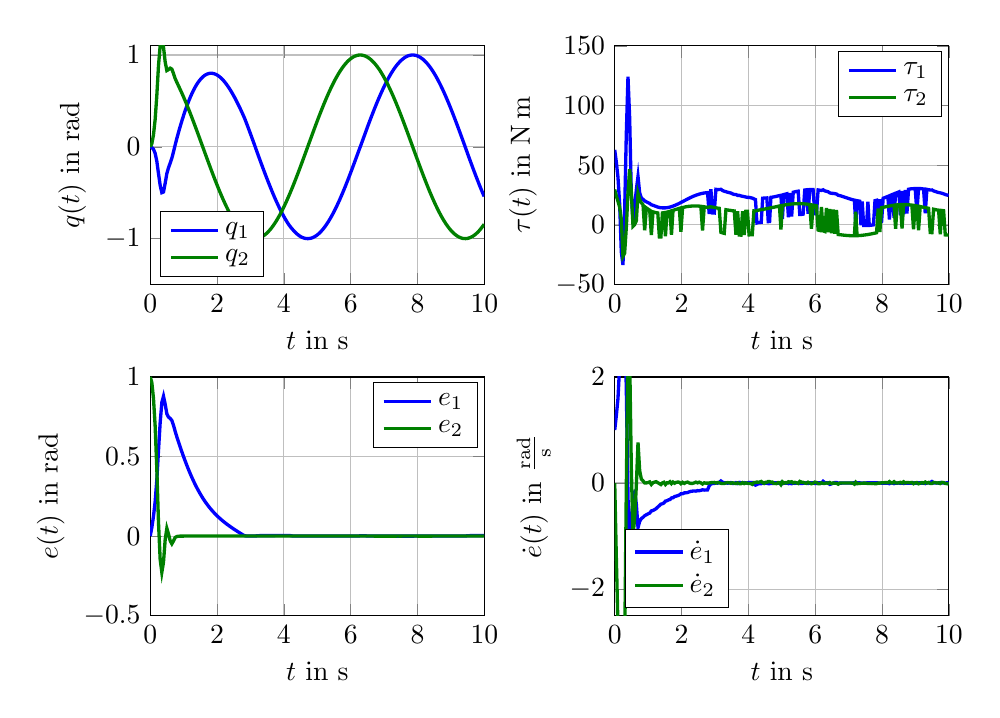
\begin{tikzpicture}

\begin{axis}[%
width=0.35\textwidth,
height=0.25\textwidth,
scale only axis,
xmin=0,
xmax=10,
xlabel={$t$ in $\mathrm{s}$},
xmajorgrids,
ymin=-1.5,
ymax=1.1,
ylabel={$q(t)$ in $\mathrm{rad}$},
ymajorgrids,
name=plot1,
legend style={at={(0.03,0.03)},anchor=south west,draw=black,fill=white,legend cell align=left}
]
\addplot [
color=blue,
solid,
line width=1.2pt
]
table[row sep=crcr]{
0 0\\
0.0469734754340576 -0.00632031829179649\\
0.0969734754340577 -0.0270440918337549\\
0.146973475434058 -0.0704875998953035\\
0.196973475434058 -0.156812657158635\\
0.246973475434058 -0.291924567589284\\
0.296973475434058 -0.419481560784783\\
0.346973475434058 -0.499384751198038\\
0.396973475434058 -0.491945898651832\\
0.446973475434058 -0.396931003408858\\
0.496973475434058 -0.291893095979682\\
0.546973475434058 -0.227542723410754\\
0.596973475434058 -0.17743664661974\\
0.646973475434058 -0.123753296345779\\
0.696960774709997 -0.0540856448572159\\
0.746960774709997 0.021773258412653\\
0.796875666311765 0.0917853921750312\\
0.846767737105723 0.158169046701825\\
0.896767339359137 0.221783045749652\\
0.946767339359137 0.28238288881527\\
0.996767339359137 0.339911018523323\\
1.04670309642092 0.394416698103635\\
1.0962655978987 0.445294761291844\\
1.14559945627848 0.492677481091908\\
1.1937044397857 0.535762789847472\\
1.24138115521621 0.575268764389105\\
1.28920457688033 0.611706894558294\\
1.3360140548672 0.644244933670955\\
1.38201518671825 0.673204137981523\\
1.42732915610165 0.698768192442836\\
1.47224082939421 0.721228095021488\\
1.51813387480573 0.741240625903316\\
1.56378151435548 0.758226359937738\\
1.60851659785493 0.772071334835013\\
1.65256973669454 0.78303419636303\\
1.69845926033513 0.791661966940517\\
1.74439394790063 0.797516052505586\\
1.79030452580486 0.800641015306367\\
1.83687793464332 0.801063727659724\\
1.88420056385082 0.798747511004859\\
1.93245637513083 0.793607871764884\\
1.98138534088319 0.785615831889007\\
2.03101309751924 0.774753797353318\\
2.08095627799577 0.761103625810322\\
2.1304377872903 0.744990593693604\\
2.17940291611027 0.726641995654192\\
2.22865818084364 0.705832482807509\\
2.27817307106154 0.682656970949797\\
2.32794450142837 0.657192246299064\\
2.37785079169497 0.629596710623812\\
2.42785079169497 0.600017286155077\\
2.47785079169496 0.568604993843296\\
2.52785079169496 0.535476718692267\\
2.57785079169495 0.500760892338125\\
2.62785079169495 0.464581071124308\\
2.67785079169494 0.42706338131659\\
2.72785079169493 0.388335431118627\\
2.77785079169493 0.348624070583341\\
2.82785079169492 0.306509972082444\\
2.87785079169492 0.260004360157712\\
2.92785079169491 0.211780438319409\\
2.97785079169491 0.162742355371706\\
3.0278507916949 0.113188838669706\\
3.0778507916949 0.0633679029739536\\
3.12785079169489 0.0133655867712655\\
3.17785079169489 -0.0376217852970143\\
3.22785079169488 -0.0886006195342584\\
3.27785079169487 -0.138560611333216\\
3.32785079169487 -0.188009925239962\\
3.37785079169486 -0.236901355844907\\
3.42785079169486 -0.285227325003042\\
3.47785079169485 -0.332723376091923\\
3.52785079169485 -0.379495586861311\\
3.57785079169484 -0.425310560599352\\
3.62782979788007 -0.470101203965342\\
3.67778831997431 -0.513919907284255\\
3.72736668054599 -0.555933790754408\\
3.77691921382158 -0.596635410422686\\
3.82609135340826 -0.635640679057179\\
3.87523042674792 -0.672986023302518\\
3.92399064516093 -0.708310854451496\\
3.97264942383006 -0.742038441486303\\
4.0205008815604 -0.773515136691791\\
4.06871124489593 -0.803545519796677\\
4.116698194706 -0.831593913170433\\
4.1651553107062 -0.857442463909213\\
4.21206242489048 -0.879621260184009\\
4.25522513734041 -0.898235230390443\\
4.29826428943344 -0.915962470431544\\
4.34168912613316 -0.932402377296095\\
4.38441362375436 -0.946979272102861\\
4.42751393350718 -0.959980762773161\\
4.47024219699147 -0.971134210373654\\
4.51203413325444 -0.980291404248003\\
4.55330447295315 -0.987630238346219\\
4.59401222119774 -0.993288576708572\\
4.63486640577313 -0.997276521618781\\
4.67330940274627 -0.999545389859861\\
4.71560486342735 -1.00032328670385\\
4.75627406880812 -0.999344916269457\\
4.7997379027444 -0.996496665585741\\
4.84316436023501 -0.991773266032406\\
4.88695952861647 -0.985084045620939\\
4.93031922128161 -0.976613986122446\\
4.97394096726878 -0.966281219221222\\
5.01715658366258 -0.954213840169789\\
5.06131234034922 -0.940008534731243\\
5.10475143603095 -0.924272399479842\\
5.15114240879323 -0.905554244558607\\
5.1986196352894 -0.884376768025541\\
5.24532713268562 -0.861586972026453\\
5.29437108518349 -0.835649802731795\\
5.34239685652401 -0.808285790473285\\
5.391579352351 -0.778338715130681\\
5.44057682275869 -0.746608195305992\\
5.48963103313765 -0.71306126274358\\
5.53857714522327 -0.677868949604567\\
5.58772172393509 -0.640968278469142\\
5.63703119716396 -0.602339983588438\\
5.68672917069612 -0.561927540716059\\
5.73664772687745 -0.519929934642594\\
5.78662416780668 -0.476585258000314\\
5.83662240326954 -0.432036572219262\\
5.88662240326956 -0.386432367208638\\
5.93662240326957 -0.339851512322663\\
5.98662240326959 -0.292438274685484\\
6.03662240326961 -0.244218356225285\\
6.08662240326962 -0.195432494480856\\
6.13662240326964 -0.146170442152491\\
6.18662240326966 -0.0965450305954266\\
6.23662240326967 -0.0471177038973554\\
6.28662240326969 0.00151898039446618\\
6.33662240326971 0.0509877432547302\\
6.38662240326972 0.100759107449522\\
6.43662240326974 0.150654446351854\\
6.48662240326976 0.20126152277946\\
6.53662240326977 0.250414043045152\\
6.58662240326979 0.298428049520819\\
6.63662240326981 0.345316962706359\\
6.68662240326982 0.392127679343442\\
6.73662240326984 0.437791392265112\\
6.78661064778198 0.482245096989174\\
6.83653800575799 0.525359527232925\\
6.88641040629761 0.567108431778515\\
6.93582454547484 0.607138555374736\\
6.98494325825149 0.645407127741543\\
7.03402354741337 0.682101730298192\\
7.0837576080304 0.717562807544132\\
7.13135748687763 0.750011793574375\\
7.17243780557435 0.776583461636561\\
7.21250192700837 0.801175696290668\\
7.25213423169075 0.824245240356497\\
7.29083526871018 0.845547239889078\\
7.33036999645199 0.865982553880959\\
7.36919750163579 0.884828267971791\\
7.4064037218678 0.901566111017786\\
7.44977127576328 0.919466049401943\\
7.49729884581975 0.937087928711376\\
7.53598462461347 0.949961282006673\\
7.57710927101186 0.962073791626603\\
7.61671994987844 0.972182540932774\\
7.65655573708434 0.980762328319287\\
7.69879741840002 0.988158931083989\\
7.74275753388478 0.993981246250562\\
7.78860771716203 0.997979693617948\\
7.83593751724949 0.999925083109714\\
7.88469051849092 0.999576136296211\\
7.93435146283592 0.996763658857984\\
7.98390410142242 0.991503347498611\\
8.03299606186776 0.983886995423637\\
8.07990601648678 0.974395837746821\\
8.12754603975372 0.962608596347518\\
8.17387464333219 0.949053915359574\\
8.22124606696587 0.933108221003423\\
8.26594124683374 0.916147280108065\\
8.31199984312091 0.896739246241706\\
8.3588140953227 0.875069049480132\\
8.40554964867512 0.851514370349743\\
8.45336291175028 0.825513752103889\\
8.50136438541207 0.797480001377451\\
8.54953828134788 0.767514106646109\\
8.59782124407076 0.735702124870707\\
8.64597747994387 0.702294932347278\\
8.69455948555231 0.666889210625639\\
8.74356785834961 0.629585502585362\\
8.7927657317259 0.590608219851682\\
8.84208415677449 0.550088641980403\\
8.89200657192542 0.507766528455668\\
8.94197969595096 0.464098252305459\\
8.99197969595093 0.41922837005454\\
9.04197969595091 0.373348542978927\\
9.09197969595088 0.326485424483356\\
9.14197969595085 0.278854744405041\\
9.19197969595082 0.230522374944262\\
9.2419796959508 0.181604424411121\\
9.29197969595077 0.132172786669927\\
9.34197969595074 0.0824989933753201\\
9.39197969595071 0.0323793027730793\\
9.44197969595069 -0.0179589320876258\\
9.49197969595066 -0.0690806494297199\\
9.54197969595063 -0.119527159801398\\
9.5919796959506 -0.169205505932314\\
9.64197969595057 -0.218303436436721\\
9.69197969595055 -0.266842397172325\\
9.74197969595052 -0.314714397073885\\
9.79197969595049 -0.361780237586748\\
9.84197969595046 -0.408061396672569\\
9.89197419966876 -0.453231483315328\\
9.94196070395594 -0.497495561766168\\
9.99174480952225 -0.540304352342543\\
};
\addlegendentry{$q_1$};

\addplot [
color=green!50!black,
solid,
line width=1.2pt
]
table[row sep=crcr]{
0 0\\
0.0469734754340576 0.0323801763143347\\
0.0969734754340577 0.129860435787076\\
0.146973475434058 0.297308984784062\\
0.196973475434058 0.559090822288292\\
0.246973475434058 0.883263345339973\\
0.296973475434058 1.10254810294153\\
0.346973475434058 1.16827577572378\\
0.396973475434058 1.08579071137771\\
0.446973475434058 0.924676676691215\\
0.496973475434058 0.830394875960034\\
0.546973475434058 0.841016438427842\\
0.596973475434058 0.856662583510026\\
0.646973475434058 0.846389690608296\\
0.696960774709997 0.796817533594228\\
0.746960774709997 0.74233607144393\\
0.796875666311765 0.701572439808967\\
0.846767737105723 0.663363527511569\\
0.896767339359137 0.624345515551985\\
0.946767339359137 0.584333169521449\\
0.996767339359137 0.54310009599411\\
1.04670309642092 0.500256214026392\\
1.0962655978987 0.45667698098303\\
1.14559945627848 0.412282149981484\\
1.1937044397857 0.367894459327305\\
1.24138115521621 0.323181166191334\\
1.28920457688033 0.277573399778796\\
1.3360140548672 0.232313769318971\\
1.38201518671825 0.187303675188466\\
1.42732915610165 0.142629445264369\\
1.47224082939421 0.098066379688997\\
1.51813387480573 0.052316741137452\\
1.56378151435548 0.0066866934070894\\
1.60851659785493 -0.0380447471618878\\
1.65256973669454 -0.0820292748779301\\
1.69845926033513 -0.12764488900764\\
1.74439394790063 -0.173056876781878\\
1.79030452580486 -0.218100734993141\\
1.83687793464332 -0.263285420222229\\
1.88420056385082 -0.308620014333068\\
1.93245637513083 -0.354134240111653\\
1.98138534088319 -0.399435773379925\\
2.03101309751924 -0.44443332267347\\
2.08095627799577 -0.488599155383349\\
2.1304377872903 -0.531141224497544\\
2.17940291611027 -0.57202829613088\\
2.22865818084364 -0.611730901907758\\
2.27817307106154 -0.650134403082622\\
2.32794450142837 -0.687111679766103\\
2.37785079169497 -0.722475344036018\\
2.42785079169497 -0.756147657298052\\
2.47785079169496 -0.787927584918723\\
2.52785079169496 -0.817723068935438\\
2.57785079169495 -0.845475776700369\\
2.62785079169495 -0.871119326867422\\
2.67785079169494 -0.894599961313006\\
2.72785079169493 -0.915842908534484\\
2.77785079169493 -0.934794925816887\\
2.82785079169492 -0.951377769644509\\
2.87785079169492 -0.965517952313781\\
2.92785079169491 -0.977379740562138\\
2.97785079169491 -0.986802975351699\\
3.0278507916949 -0.993757154083667\\
3.0778507916949 -0.998199367680274\\
3.12785079169489 -1.000118100374\\
3.17785079169489 -0.999554050981952\\
3.22785079169488 -0.996484599950843\\
3.27785079169487 -0.99093603919897\\
3.32785079169487 -0.982906198399579\\
3.37785079169486 -0.972431934682722\\
3.42785079169486 -0.95949708635058\\
3.47785079169485 -0.944251120446024\\
3.52785079169485 -0.926630824276387\\
3.57785079169484 -0.906641790140353\\
3.62782979788007 -0.8844031833884\\
3.67778831997431 -0.859928662942097\\
3.72736668054599 -0.833518903046293\\
3.77691921382158 -0.805106368836581\\
3.82609135340826 -0.774963879847186\\
3.87523042674792 -0.742992782111143\\
3.92399064516093 -0.709479664650458\\
3.97264942383006 -0.674378485183347\\
4.0205008815604 -0.638282428313245\\
4.06871124489593 -0.600441017208818\\
4.116698194706 -0.561404267966328\\
4.1651553107062 -0.520635684339841\\
4.21206242489048 -0.480019403772923\\
4.25522513734041 -0.441736209016257\\
4.29826428943344 -0.402719093300347\\
4.34168912613316 -0.362627534162072\\
4.38441362375436 -0.322567757068972\\
4.42751393350718 -0.281449576360196\\
4.47024219699147 -0.240125610770008\\
4.51203413325444 -0.199384809881457\\
4.55330447295315 -0.158837789407429\\
4.59401222119774 -0.118518175264766\\
4.63486640577313 -0.0778459917702662\\
4.67330940274627 -0.0395417773405039\\
4.71560486342735 0.00276915899889639\\
4.75627406880812 0.0434444141859095\\
4.7997379027444 0.0867914557521447\\
4.84316436023501 0.129942580082296\\
4.88695952861647 0.173174293834576\\
4.93031922128161 0.215687555223838\\
4.97394096726878 0.258053763547482\\
5.01715658366258 0.299587035119213\\
5.06131234034922 0.341355112504133\\
5.10475143603095 0.381865102220009\\
5.15114240879323 0.424310759510842\\
5.1986196352894 0.466777897910955\\
5.24532713268562 0.507606611766433\\
5.29437108518349 0.549214704249983\\
5.34239685652401 0.588732822744014\\
5.391579352351 0.627760880074126\\
5.44057682275869 0.665142958789729\\
5.48963103313765 0.700952632916878\\
5.53857714522327 0.734934096935974\\
5.58772172393509 0.76737937788878\\
5.63703119716396 0.798076628884092\\
5.68672917069612 0.827075781747612\\
5.73664772687745 0.854083628136307\\
5.78662416780668 0.878982082380211\\
5.83662240326954 0.90169393859637\\
5.88662240326956 0.922222392856635\\
5.93662240326957 0.940300779552662\\
5.98662240326959 0.956133194815146\\
6.03662240326961 0.969588258688267\\
6.08662240326962 0.980652714346777\\
6.13662240326964 0.98920955414638\\
6.18662240326966 0.995279703206752\\
6.23662240326967 0.998746669018398\\
6.28662240326969 0.999772163470769\\
6.33662240326971 0.998402052973801\\
6.38662240326972 0.994463833134051\\
6.43662240326974 0.988064611665903\\
6.48662240326976 0.979219948471954\\
6.53662240326977 0.967930834721106\\
6.58662240326979 0.954166244480849\\
6.63662240326981 0.938037541238595\\
6.68662240326982 0.919695249058408\\
6.73662240326984 0.899209703754287\\
6.78661064778198 0.876223136961668\\
6.83653800575799 0.851116073715459\\
6.88641040629761 0.823929257574073\\
6.93582454547484 0.794806276189357\\
6.98494325825149 0.764066182640237\\
7.03402354741337 0.731442509832695\\
7.0837576080304 0.69674662863729\\
7.13135748687763 0.661566989621661\\
7.17243780557435 0.630167516028765\\
7.21250192700837 0.598716835445913\\
7.25213423169075 0.566527549198921\\
7.29083526871018 0.534177707359249\\
7.33036999645199 0.500322978729579\\
7.36919750163579 0.466065859655569\\
7.4064037218678 0.432764352846866\\
7.44977127576328 0.39333979924876\\
7.49729884581975 0.349317424106889\\
7.53598462461347 0.312609790098782\\
7.57710927101186 0.273144935248992\\
7.61671994987844 0.234726915854434\\
7.65655573708434 0.19581263477664\\
7.69879741840002 0.154243875312037\\
7.74275753388478 0.110692985148954\\
7.78860771716203 0.0651046382384844\\
7.83593751724949 0.0178811142140073\\
7.88469051849092 -0.0308136526682363\\
7.93435146283592 -0.0803238019805663\\
7.98390410142242 -0.12953638515311\\
8.03299606186776 -0.177949796307657\\
8.07990601648678 -0.223872084043635\\
8.12754603975372 -0.270016246166765\\
8.17387464333219 -0.314331978364796\\
8.22124606696587 -0.358963801255343\\
8.26594124683374 -0.400316358962396\\
8.31199984312091 -0.44210019710887\\
8.3588140953227 -0.483612257886788\\
8.40554964867512 -0.523958461812771\\
8.45336291175028 -0.564112595658254\\
8.50136438541207 -0.603072533796897\\
8.54953828134788 -0.640780759371605\\
8.59782124407076 -0.677085280280953\\
8.64597747994387 -0.712020168805539\\
8.69455948555231 -0.745378167726193\\
8.74356785834961 -0.777197504746584\\
8.7927657317259 -0.807209430737975\\
8.84208415677449 -0.835419037223789\\
8.89200657192542 -0.861735328459004\\
8.94197969595096 -0.885935909619661\\
8.99197969595093 -0.908026363858972\\
9.04197969595091 -0.927839558466058\\
9.09197969595088 -0.945267942695446\\
9.14197969595085 -0.960430996048044\\
9.19197969595082 -0.973161941597602\\
9.2419796959508 -0.983454649881324\\
9.29197969595077 -0.99141233567162\\
9.34197969595074 -0.99682388853379\\
9.39197969595071 -0.999678958959472\\
9.44197969595069 -1.00003362420405\\
9.49197969595066 -0.997962336464399\\
9.54197969595063 -0.993357113454534\\
9.5919796959506 -0.986264709686612\\
9.64197969595057 -0.976724468588219\\
9.69197969595055 -0.964724150235981\\
9.74197969595052 -0.950295384890106\\
9.79197969595049 -0.933586118426375\\
9.84197969595046 -0.914490687217394\\
9.89197419966876 -0.893095987960206\\
9.94196070395594 -0.869461131064867\\
9.99174480952225 -0.843737899862484\\
};
\addlegendentry{$q_2$};

\end{axis}

\begin{axis}[%
width=0.35\textwidth,
height=0.25\textwidth,
scale only axis,
xmin=0,
xmax=10,
xlabel={$t$ in $\mathrm{s}$},
xmajorgrids,
ymin=-0.5,
ymax=1,
ylabel={$e(t)$ in $\mathrm{rad}$},
ymajorgrids,
name=plot3,
at=(plot1.below south west),
anchor=above north west,
legend style={draw=black,fill=white,legend cell align=left}
]
\addplot [
color=blue,
solid,
line width=1.2pt
]
table[row sep=crcr]{
0 0\\
0.0469734754340576 0.0532765210780949\\
0.0969734754340577 0.123865651299229\\
0.146973475434058 0.216932512564983\\
0.196973475434058 0.352514887017883\\
0.246973475434058 0.536394960983202\\
0.296973475434058 0.712109069047606\\
0.346973475434058 0.83943795795657\\
0.396973475434058 0.878574847985463\\
0.446973475434058 0.829169324296718\\
0.496973475434058 0.768660417724918\\
0.546973475434058 0.747647376004623\\
0.596973475434058 0.739578639296025\\
0.646973475434058 0.72652756688068\\
0.696960774709997 0.695975832673234\\
0.746960774709997 0.65763858961061\\
0.796875666311765 0.623390456804122\\
0.846767737105723 0.590974198613288\\
0.896767339359137 0.559530320382588\\
0.946767339359137 0.529147985089494\\
0.996767339359137 0.499808958606311\\
1.04670309642092 0.471361372437702\\
1.0962655978987 0.444212478123407\\
1.14559945627848 0.418280060402398\\
1.1937044397857 0.39397659593237\\
1.24138115521621 0.37096292691649\\
1.28920457688033 0.348907437360894\\
1.3360140548672 0.328320081064403\\
1.38201518671825 0.30902956017477\\
1.42732915610165 0.29095803311936\\
1.47224082939421 0.273919241754656\\
1.51813387480573 0.257373027616497\\
1.56378151435548 0.241749036366373\\
1.60851659785493 0.227217340087127\\
1.65256973669454 0.213624221042827\\
1.69845926033513 0.200200182210611\\
1.74439394790063 0.187453683582577\\
1.79030452580486 0.175363641545314\\
1.83687793464332 0.163744925637837\\
1.88420056385082 0.152542050761698\\
1.93245637513083 0.141702870373457\\
1.98138534088319 0.131270045339425\\
2.03101309751924 0.121202444167691\\
2.08095627799577 0.11156278613457\\
2.1304377872903 0.102454914094417\\
2.17940291611027 0.0938034658613204\\
2.22865818084364 0.0854688752152321\\
2.27817307106154 0.0774122204356061\\
2.32794450142837 0.069605497921182\\
2.37785079169497 0.0620321414344208\\
2.42785079169497 0.0546496003208625\\
2.47785079169496 0.0474636007780851\\
2.52785079169496 0.040453733430324\\
2.57785079169495 0.0335918910941513\\
2.62785079169495 0.0268584399446237\\
2.67785079169494 0.0202345145480746\\
2.72785079169493 0.0137028377503497\\
2.77785079169493 0.00714968499525787\\
2.82785079169492 0.00211002110022146\\
2.87785079169492 0.000690481372249085\\
2.92785079169491 0.000337650221271829\\
2.97785079169491 0.000268795427308649\\
3.0278507916949 0.000307931405210168\\
3.0778507916949 0.000330803559652482\\
3.12785079169489 0.000375842628341637\\
3.17785079169489 0.00137159114552157\\
3.22785079169488 0.00244940843830838\\
3.27785079169487 0.0027237164538651\\
3.32785079169487 0.00282686807192065\\
3.37785079169486 0.00283499758962441\\
3.42785079169486 0.00286270965675273\\
3.47785079169485 0.00276626814034425\\
3.52785079169485 0.00277070723598094\\
3.57785079169484 0.00275952530480839\\
3.62782979788007 0.00279873100577949\\
3.67778831997431 0.00305063825790808\\
3.72736668054599 0.00308925827664885\\
3.77691921382158 0.0031950233004383\\
3.82609135340826 0.0033559634293765\\
3.87523042674792 0.00341003130793271\\
3.92399064516093 0.00332869426816651\\
3.97264942383006 0.00339429393727653\\
4.0205008815604 0.00347234079964787\\
4.06871124489593 0.00365150829220939\\
4.116698194706 0.00383280331038849\\
4.1651553107062 0.00347528016927212\\
4.21206242489048 0.00219530412658897\\
4.25522513734041 0.000927231866340028\\
4.29826428943344 0.000493584752995324\\
4.34168912613316 0.00032833809196009\\
4.38441362375436 0.000282796452402923\\
4.42751393350718 0.000283986106134781\\
4.47024219699147 0.000308769472171178\\
4.51203413325444 0.00029538535045126\\
4.55330447295315 0.000257514067506071\\
4.59401222119774 0.000286927180130681\\
4.63486640577313 0.000279891828667389\\
4.67330940274627 0.000308899376475602\\
4.71560486342735 0.000328457651265657\\
4.75627406880812 0.000307712226735757\\
4.7997379027444 0.000309157722485409\\
4.84316436023501 0.000312186080034693\\
4.88695952861647 0.000282826476728726\\
4.93031922128161 0.000266944689536142\\
4.97394096726878 0.00029139042502635\\
5.01715658366258 0.000297126210894283\\
5.06131234034922 0.000267188886261316\\
5.10475143603095 0.000264098103483046\\
5.15114240879323 0.000272320404466342\\
5.1986196352894 0.00027623030146906\\
5.24532713268562 0.00026895751568945\\
5.29437108518349 0.000275036101682113\\
5.34239685652401 0.000262922372390562\\
5.391579352351 0.00025716282423105\\
5.44057682275869 0.000226544272383555\\
5.48963103313765 0.000210823351596612\\
5.53857714522327 0.000185226593980237\\
5.58772172393509 0.000226850936152601\\
5.63703119716396 0.00021969662369814\\
5.68672917069612 0.000213483633208389\\
5.73664772687745 0.00019763058779787\\
5.78662416780668 0.000180432350558757\\
5.83662240326954 0.000168524487338562\\
5.88662240326956 0.000182094027636359\\
5.93662240326957 0.000184438220282412\\
5.98662240326959 0.000203390451788799\\
6.03662240326961 0.000146096877873952\\
6.08662240326962 0.000132913557722492\\
6.13662240326964 0.000131686895886773\\
6.18662240326966 0.000132121837981128\\
6.23662240326967 0.000571623700089806\\
6.28662240326969 0.00191810892821138\\
6.33662240326971 0.00242392465458539\\
6.38662240326972 0.00249363769291686\\
6.43662240326974 0.00218129793384239\\
6.48662240326976 0.000775210884096489\\
6.53662240326977 0.000318693380801482\\
6.58662240326979 0.000373988405552084\\
6.63662240326981 0.000807527238705974\\
6.68662240326982 0.000454131653603085\\
6.73662240326984 0.000266489709074891\\
6.78661064778198 0.00018364238081825\\
6.83653800575799 0.00018301644306673\\
6.88641040629761 0.00019288967065334\\
6.93582454547484 0.000146795033920677\\
6.98494325825149 0.000154118504262057\\
7.03402354741337 0.000150121226221045\\
7.0837576080304 0.00019189169895828\\
7.13135748687763 6.102665846619e-05\\
7.17243780557435 1.75823360915039e-05\\
7.21250192700837 3.55095540944816e-05\\
7.25213423169075 4.58449601024036e-05\\
7.29083526871018 3.23743338883631e-05\\
7.33036999645199 3.64188697478118e-05\\
7.36919750163579 -5.27001682248951e-05\\
7.4064037218678 -6.81261805803857e-05\\
7.44977127576328 -5.28051355971337e-05\\
7.49729884581975 -2.76881673707541e-05\\
7.53598462461347 -9.7694621372324e-05\\
7.57710927101186 -0.000158715135899268\\
7.61671994987844 -0.000197303737269894\\
7.65655573708434 -0.000187602662686581\\
7.69879741840002 -0.000175856292536136\\
7.74275753388478 -0.000160272570474795\\
7.78860771716203 -0.000115807187284989\\
7.83593751724949 -8.7873766914659e-05\\
7.88469051849092 -4.7617036659009e-05\\
7.93435146283592 8.42451705385106e-06\\
7.98390410142242 6.85941017919411e-05\\
8.03299606186776 0.000132666060349784\\
8.07990601648678 0.000191617259476362\\
8.12754603975372 0.000205440614497787\\
8.17387464333219 0.000215152968220833\\
8.22124606696587 0.000204858161362842\\
8.26594124683374 0.000190662334254688\\
8.31199984312091 0.000191303385482899\\
8.3588140953227 0.000186469109239029\\
8.40554964867512 0.00018952274874906\\
8.45336291175028 0.000171061654195115\\
8.50136438541207 0.000184992032213893\\
8.54953828134788 0.000183007298354854\\
8.59782124407076 0.000171994078331239\\
8.64597747994387 0.000131226681964858\\
8.69455948555231 0.000143210600749621\\
8.74356785834961 0.000148003446162059\\
8.7927657317259 0.000161280670967656\\
8.84208415677449 0.000186570125661256\\
8.89200657192542 0.000156042180485372\\
8.94197969595096 0.000161158753038071\\
8.99197969595093 0.000184323825996702\\
9.04197969595091 0.000169120414857726\\
9.09197969595088 0.000203608789432375\\
9.14197969595085 0.000189106299928909\\
9.19197969595082 0.000178828889356747\\
9.2419796959508 0.000177499688427646\\
9.29197969595077 0.000235497555498065\\
9.34197969595074 0.000204699222320304\\
9.39197969595071 0.000413082036532904\\
9.44197969595069 0.000758045225129702\\
9.49197969595066 0.00192948415422302\\
9.54197969595063 0.00259355905443817\\
9.5919796959506 0.00278174281791593\\
9.64197969595057 0.00280548369084985\\
9.69197969595055 0.00280888744768071\\
9.74197969595052 0.00280527663878544\\
9.79197969595049 0.00277511680314974\\
9.84197969595046 0.00285760137617697\\
9.89197419966876 0.00284671923179136\\
9.94196070395594 0.00306226203669152\\
9.99174480952225 0.00322839499307581\\
};
\addlegendentry{$e_1$};

\addplot [
color=green!50!black,
solid,
line width=1.2pt
]
table[row sep=crcr]{
0 1\\
0.0469734754340576 0.966516772835022\\
0.0969734754340577 0.865441320276216\\
0.146973475434058 0.691909842146142\\
0.196973475434058 0.421572543616705\\
0.246973475434058 0.086393411844662\\
0.296973475434058 -0.14632159138274\\
0.346973475434058 -0.227869578076589\\
0.396973475434058 -0.163555353382162\\
0.446973475434058 -0.0229172664514083\\
0.496973475434058 0.0486346576256554\\
0.546973475434058 0.0130861024594983\\
0.596973475434058 -0.0296218468652493\\
0.646973475434058 -0.0484779293332049\\
0.696960774709997 -0.0300209590156002\\
0.746960774709997 -0.00857893126360132\\
0.796875666311765 -0.00262787474178805\\
0.846767737105723 -0.000955497669885785\\
0.896767339359137 -0.000206569560703418\\
0.946767339359137 -2.36276693832416e-05\\
0.996767339359137 -8.04278333631503e-05\\
1.04670309642092 0.000171935231540243\\
1.0962655978987 0.000244096477683975\\
1.14559945627848 0.000217980436252208\\
1.1937044397857 0.000323783742919248\\
1.24138115521621 0.000308534369522273\\
1.28920457688033 0.000311657954527256\\
1.3360140548672 0.000317467003268346\\
1.38201518671825 0.000358154191439974\\
1.42732915610165 0.000346071641186885\\
1.47224082939421 0.00032964719902305\\
1.51813387480573 0.000321372466768631\\
1.56378151435548 0.000328061502130119\\
1.60851659785493 0.000333420317642642\\
1.65256973669454 0.000346969486537549\\
1.69845926033513 0.000328444345900597\\
1.74439394790063 0.000329869656718496\\
1.79030452580486 0.000351085616081465\\
1.83687793464332 0.00033245385343883\\
1.88420056385082 0.000321182557805888\\
1.93245637513083 0.000306858976973634\\
1.98138534088319 0.000286317487712628\\
2.03101309751924 0.000290988190990271\\
2.08095627799577 0.000282318213843946\\
2.1304377872903 0.000258835140068414\\
2.17940291611027 0.000303498104243571\\
2.22865818084364 0.000304568821453355\\
2.27817307106154 0.000292249704789249\\
2.32794450142837 0.000260139041062923\\
2.37785079169497 0.000222250584276051\\
2.42785079169497 0.000230156672554438\\
2.47785079169496 0.00023507719680993\\
2.52785079169496 0.000224375164085133\\
2.57785079169495 0.000214217868915845\\
2.62785079169495 0.000207616669236077\\
2.67785079169494 0.000214925461531457\\
2.72785079169493 0.00022004383262586\\
2.77785079169493 0.000222812579229958\\
2.82785079169492 0.000192351438399685\\
2.87785079169492 9.66973169441721e-05\\
2.92785079169491 0.000135699130394018\\
2.97785079169491 0.000178748649768856\\
3.0278507916949 0.00021878885434079\\
3.0778507916949 0.00023019241184663\\
3.12785079169489 0.000212518272346474\\
3.17785079169489 0.000211305261556105\\
3.22785079169488 0.000202527028369093\\
3.27785079169487 0.000204825403050779\\
3.32785079169487 0.00020215580186056\\
3.37785079169486 0.000211311607326792\\
3.42785079169486 0.000189928032483411\\
3.47785079169485 0.000255195183509915\\
3.52785079169485 0.000305630259037626\\
3.57785079169484 0.000302657932375161\\
3.62782979788007 0.000305678151631961\\
3.67778831997431 0.000270248242114524\\
3.72736668054599 0.000234484069525531\\
3.77691921382158 0.0002284234733122\\
3.82609135340826 0.000227770979482789\\
3.87523042674792 0.000249225461564251\\
3.92399064516093 0.000254627145967468\\
3.97264942383006 0.000282925717500437\\
4.0205008815604 0.00029019286314913\\
4.06871124489593 0.000299725212265289\\
4.116698194706 0.000323574123394454\\
4.1651553107062 0.000308816788996191\\
4.21206242489048 0.000307311329213023\\
4.25522513734041 0.000331229677931588\\
4.29826428943344 0.000330326863613006\\
4.34168912613316 0.000359697552624438\\
4.38441362375436 0.000440789879012415\\
4.42751393350718 0.000412039979521162\\
4.47024219699147 0.000338281458300033\\
4.51203413325444 0.00036771778896863\\
4.55330447295315 0.000423448672657395\\
4.59401222119774 0.000417692480851217\\
4.63486640577313 0.000401042372930926\\
4.67330940274627 0.000472146084907442\\
4.71560486342735 0.000446718500705114\\
4.75627406880812 0.000426589204733131\\
4.7997379027444 0.000446432674819863\\
4.84316436023501 0.000460360604169791\\
4.88695952861647 0.000510935163394122\\
4.93031922128161 0.000521729232689727\\
4.97394096726878 0.000526302703373838\\
5.01715658366258 0.000484461077717047\\
5.06131234034922 0.000531130140203617\\
5.10475143603095 0.00050730654868858\\
5.15114240879323 0.000500537184262961\\
5.1986196352894 0.000518837789184434\\
5.24532713268562 0.000459602303383377\\
5.29437108518349 0.000466111567419603\\
5.34239685652401 0.000418299317214488\\
5.391579352351 0.000402393255654387\\
5.44057682275869 0.000375208505758895\\
5.48963103313765 0.000363452068100178\\
5.53857714522327 0.000419404154835323\\
5.58772172393509 0.000377369423145257\\
5.63703119716396 0.0003287568852548\\
5.68672917069612 0.000255662158349934\\
5.73664772687745 0.000245542688319111\\
5.78662416780668 0.000243964832691956\\
5.83662240326954 0.000242860380263998\\
5.88662240326956 0.000171626241277978\\
5.93662240326957 0.000244954992303037\\
5.98662240326959 0.000213380667256402\\
6.03662240326961 0.000168789348533482\\
6.08662240326962 9.09186640362103e-05\\
6.13662240326964 6.93155173270288e-05\\
6.18662240326966 6.17211421638508e-05\\
6.23662240326967 0.000169474818645821\\
6.28662240326969 0.00022192972027979\\
6.33662240326971 0.00017052512513005\\
6.38662240326972 0.000191318474057733\\
6.43662240326974 0.000186993578752181\\
6.48662240326976 0.000157996067620347\\
6.53662240326977 0.000125514302210306\\
6.58662240326979 0.000148872307650372\\
6.63662240326981 0.000151052520819928\\
6.68662240326982 2.18387866971481e-05\\
6.73662240326984 -0.000262935563706601\\
6.78661064778198 -0.000287915937944194\\
6.83653800575799 -0.000348752536178831\\
6.88641040629761 -0.000418959713732403\\
6.93582454547484 -0.000322479514412555\\
6.98494325825149 -0.000357679777027831\\
7.03402354741337 -0.000325274984882773\\
7.0837576080304 -0.000450576864439056\\
7.13135748687763 -0.000211741401801913\\
7.17243780557435 -0.000174802975203892\\
7.21250192700837 -0.000335181625559455\\
7.25213423169075 -0.000361313303859467\\
7.29083526871018 -0.0003283690525131\\
7.33036999645199 -0.000311840017839682\\
7.36919750163579 -4.84837800793225e-05\\
7.4064037218678 1.89455074683931e-05\\
7.44977127576328 -4.69233056104024e-05\\
7.49729884581975 -0.000149691359988047\\
7.53598462461347 5.48311162317239e-05\\
7.57710927101186 0.00020353396179934\\
7.61671994987844 0.000314992481077331\\
7.65655573708434 0.00033324818673483\\
7.69879741840002 0.000318228470316873\\
7.74275753388478 0.000301934885987759\\
7.78860771716203 0.000222723238109068\\
7.83593751724949 0.000162023362484057\\
7.88469051849092 0.000109594519389217\\
7.93435146283592 4.04674447746778e-05\\
7.98390410142242 -2.08787528795107e-05\\
8.03299606186776 -0.000110041423765694\\
8.07990601648678 -0.000135265265150647\\
8.12754603975372 -0.000148759392628317\\
8.17387464333219 -0.000133021144021583\\
8.22124606696587 -9.98369203238925e-05\\
8.26594124683374 -8.94042835584141e-05\\
8.31199984312091 -7.12505734385971e-05\\
8.3588140953227 -4.85500962967844e-05\\
8.40554964867512 -6.48949957519074e-05\\
8.45336291175028 -1.91162045685145e-05\\
8.50136438541207 -2.8252381300109e-05\\
8.54953828134788 -3.21159994662867e-05\\
8.59782124407076 -3.30853398416986e-05\\
8.64597747994387 0.000263545294787781\\
8.69455948555231 0.000349477652541563\\
8.74356785834961 0.000386259088255514\\
8.7927657317259 0.000369051696235245\\
8.84208415677449 0.000435689520598692\\
8.89200657192542 0.000332599047051296\\
8.94197969595096 0.000236638284510371\\
8.99197969595093 0.000230686290571436\\
9.04197969595091 0.000216491087477455\\
9.09197969595088 0.000136060078373523\\
9.14197969595085 0.00015263568385171\\
9.19197969595082 0.000137299283893721\\
9.2419796959508 0.000115780482444428\\
9.29197969595077 0.000217074248080484\\
9.34197969595074 0.000249707034633229\\
9.39197969595071 0.00021677383264207\\
9.44197969595069 0.000181570402512543\\
9.49197969595066 0.000219523409780709\\
9.54197969595063 0.000217378565051773\\
9.5919796959506 0.000210385082311304\\
9.64197969595057 0.000220176553443419\\
9.69197969595055 0.000210642947210071\\
9.74197969595052 0.000183443806633821\\
9.79197969595049 0.000250528592174559\\
9.84197969595046 0.000264301535270239\\
9.89197419966876 0.000261420819451796\\
9.94196070395594 0.000245558195499873\\
9.99174480952225 0.000204014332594538\\
};
\addlegendentry{$e_2$};

\end{axis}

\begin{axis}[%
width=0.35\textwidth,
height=0.25\textwidth,
scale only axis,
xmin=0,
xmax=10,
xlabel={$t$ in $\mathrm{s}$},
xmajorgrids,
ymin=-2.5,
ymax=2,
ylabel={$\dot{e}(t)$ in $\mathrm{\frac{rad}{s}}$},
ymajorgrids,
name=plot2,
at=(plot3.right of south east),
anchor=left of south west,
legend style={at={(0.03,0.03)},anchor=south west,draw=black,fill=white,legend cell align=left}
]
\addplot [
color=blue,
solid,
line width=1.2pt
]
table[row sep=crcr]{
0 1\\
0.0469734754340576 1.26146609737587\\
0.0969734754340577 1.58829546221262\\
0.146973475434058 2.20482462807992\\
0.196973475434058 3.29057163293317\\
0.246973475434058 3.72819086223851\\
0.296973475434058 3.17599378870207\\
0.346973475434058 1.77129152148961\\
0.396973475434058 -0.254002694057177\\
0.446973475434058 -1.34353445171103\\
0.496973475434058 -0.87826774981078\\
0.546973475434058 -0.199642650055886\\
0.596973475434058 -0.167546549760879\\
0.646973475434058 -0.39638907054621\\
0.696960774709997 -0.840682221500538\\
0.746960774709997 -0.722408450480425\\
0.796875666311765 -0.669241360273341\\
0.846767737105723 -0.646889719725198\\
0.896767339359137 -0.6156131567769\\
0.946767339359137 -0.598057966471049\\
0.996767339359137 -0.580980505689829\\
1.04670309642092 -0.56601542821897\\
1.0962655978987 -0.525857564184362\\
1.14559945627848 -0.517826961483587\\
1.1937044397857 -0.500722491484262\\
1.24138115521621 -0.481837717552452\\
1.28920457688033 -0.452573611159046\\
1.3360140548672 -0.425111141382333\\
1.38201518671825 -0.397480091628254\\
1.42732915610165 -0.390249006519262\\
1.47224082939421 -0.376073605284823\\
1.51813387480573 -0.34030691558303\\
1.56378151435548 -0.334377852828195\\
1.60851659785493 -0.317524170686094\\
1.65256973669454 -0.310311971228119\\
1.69845926033513 -0.280386355282283\\
1.74439394790063 -0.277651637015616\\
1.79030452580486 -0.254635579288253\\
1.83687793464332 -0.247974656872074\\
1.88420056385082 -0.23772448854797\\
1.93245637513083 -0.225306961301347\\
1.98138534088319 -0.202855717029518\\
2.03101309751924 -0.203216091162947\\
2.08095627799577 -0.185716391246254\\
2.1304377872903 -0.184229715636905\\
2.17940291611027 -0.17948554168075\\
2.22865818084364 -0.166355597157108\\
2.27817307106154 -0.157173106119778\\
2.32794450142837 -0.152067398424786\\
2.37785079169497 -0.150666835282359\\
2.42785079169497 -0.15195106897082\\
2.47785079169496 -0.143196033019753\\
2.52785079169496 -0.145113541996638\\
2.57785079169495 -0.137247785645836\\
2.62785079169495 -0.126629278625015\\
2.67785079169494 -0.132954009129436\\
2.72785079169493 -0.129950543414779\\
2.77785079169493 -0.128767851280054\\
2.82785079169492 -0.0536040386835813\\
2.87785079169492 -0.0169165023099886\\
2.92785079169491 -0.00994270624798099\\
2.97785079169491 -0.00744201366245401\\
3.0278507916949 0.000915241318958815\\
3.0778507916949 -0.00179256360127056\\
3.12785079169489 0.0125475934118515\\
3.17785079169489 0.0391828532011854\\
3.22785079169488 0.0143413750473124\\
3.27785079169487 0.00525522924906019\\
3.32785079169487 0.00216192940477578\\
3.37785079169486 -0.00226419739735528\\
3.42785079169486 0.000815407256622991\\
3.47785079169485 0.00852446829365905\\
3.52785079169485 -0.00802564421868501\\
3.57785079169484 -0.00569865703666295\\
3.62782979788007 0.00825839694106778\\
3.67778831997431 -0.00828869680252509\\
3.72736668054599 0.0117314556766855\\
3.77691921382158 0.00647621746533189\\
3.82609135340826 0.000430518820099812\\
3.87523042674792 0.00819708775725869\\
3.92399064516093 0.00142504225697382\\
3.97264942383006 0.00279451631054328\\
4.0205008815604 0.0116013854683223\\
4.06871124489593 0.0086507654217417\\
4.116698194706 0.00922623942521295\\
4.1651553107062 -0.021274911803598\\
4.21206242489048 -0.0398233054989077\\
4.25522513734041 -0.0271472753371826\\
4.29826428943344 -0.013141207390976\\
4.34168912613316 -0.0124875117877072\\
4.38441362375436 -0.0129687255859018\\
4.42751393350718 -0.000704811322087218\\
4.47024219699147 0.00618740838357962\\
4.51203413325444 -0.00353109109287872\\
4.55330447295315 -0.00433092208186506\\
4.59401222119774 -0.0112050816727938\\
4.63486640577313 -0.012130037651973\\
4.67330940274627 -0.00484095682067079\\
4.71560486342735 -0.00697470165030148\\
4.75627406880812 0.00316245816599989\\
4.7997379027444 0.00491053811239138\\
4.84316436023501 0.00430916627069372\\
4.88695952861647 -0.00190177824006169\\
4.93031922128161 -0.00184773825108653\\
4.97394096726878 0.0117687692622908\\
5.01715658366258 -0.0119833962044883\\
5.06131234034922 0.00251688032967401\\
5.10475143603095 -0.00256514154945725\\
5.15114240879323 -0.000851150543838775\\
5.1986196352894 -0.0112857867714486\\
5.24532713268562 -0.00655439479018438\\
5.29437108518349 -0.0127562313246626\\
5.34239685652401 -0.0014742222820664\\
5.391579352351 -0.00629451267604186\\
5.44057682275869 -0.000917326556152842\\
5.48963103313765 0.001697945412103\\
5.53857714522327 -0.00820235083153809\\
5.58772172393509 -0.00927798823790205\\
5.63703119716396 -0.00553763876449154\\
5.68672917069612 0.000812784549572565\\
5.73664772687745 0.00474223520644512\\
5.78662416780668 -0.0080279947075379\\
5.83662240326954 0.000873451506373302\\
5.88662240326956 0.00653441374063901\\
5.93662240326957 0.00226165947668444\\
5.98662240326959 -0.00844472287598463\\
6.03662240326961 -0.00793424461260461\\
6.08662240326962 0.00615697929456405\\
6.13662240326964 0.00575013905271626\\
6.18662240326966 -0.00253778398864324\\
6.23662240326967 0.0330536917224429\\
6.28662240326969 0.00816358323547206\\
6.33662240326971 0.00379443099958732\\
6.38662240326972 0.00487603097489941\\
6.43662240326974 -0.0245452490692166\\
6.48662240326976 -0.0137974485652954\\
6.53662240326977 -0.00404686448377056\\
6.58662240326979 0.00821582090801154\\
6.63662240326981 0.0110966387704681\\
6.68662240326982 -0.0012952903629263\\
6.73662240326984 -0.00264303993611292\\
6.78661064778198 -0.00119878706311138\\
6.83653800575799 0.000192482875171485\\
6.88641040629761 -0.000747853996692416\\
6.93582454547484 -0.000879413734246493\\
6.98494325825149 0.000206897476264012\\
7.03402354741337 -4.68106724680339e-05\\
7.0837576080304 -0.00130287596618461\\
7.13135748687763 0.000682612280418882\\
7.17243780557435 0.00769528913948259\\
7.21250192700837 -0.00825390679189209\\
7.25213423169075 0.00565097442724705\\
7.29083526871018 0.00487811574555075\\
7.33036999645199 0.00378837409647592\\
7.36919750163579 0.00105220381699939\\
7.4064037218678 0.00207216566595908\\
7.44977127576328 0.000907942347734725\\
7.49729884581975 -0.000156606989097086\\
7.53598462461347 0.00241911293064884\\
7.57710927101186 0.00398019617039452\\
7.61671994987844 0.00420660457759409\\
7.65655573708434 0.00387999311015613\\
7.69879741840002 0.00426187376209192\\
7.74275753388478 0.00378173918206516\\
7.78860771716203 0.00516942103048762\\
7.83593751724949 0.00538917885333404\\
7.88469051849092 0.00103945996177796\\
7.93435146283592 0.00185001872056061\\
7.98390410142242 -0.00171687003311857\\
8.03299606186776 -0.000950451052397244\\
8.07990601648678 -0.00405013866284396\\
8.12754603975372 -0.00319802353665682\\
8.17387464333219 -0.0028741596489375\\
8.22124606696587 -0.0120088743889674\\
8.26594124683374 -0.000726037388334544\\
8.31199984312091 -0.000646153647259062\\
8.3588140953227 -0.0106454520619452\\
8.40554964867512 -0.000564937706808322\\
8.45336291175028 -0.00170327202452503\\
8.50136438541207 -0.000107804702080716\\
8.54953828134788 -0.00542838279783031\\
8.59782124407076 0.000280254360378263\\
8.64597747994387 -0.00936124429172214\\
8.69455948555231 0.000298080297037151\\
8.74356785834961 -0.00439051242664534\\
8.7927657317259 -0.00372810208993224\\
8.84208415677449 -0.00132659805123281\\
8.89200657192542 -0.00380399788253671\\
8.94197969595096 0.00479447861415849\\
8.99197969595093 -0.0016644016870212\\
9.04197969595091 -0.00517653900886594\\
9.09197969595088 0.00536942545559926\\
9.14197969595085 0.00694693019970949\\
9.19197969595082 -0.00383688603739074\\
9.2419796959508 0.00222580169921172\\
9.29197969595077 -0.00947261374543107\\
9.34197969595074 0.00635741420376412\\
9.39197969595071 0.00103011582796408\\
9.44197969595069 0.0117852391908948\\
9.49197969595066 0.0287324649409639\\
9.54197969595063 0.00297007351462464\\
9.5919796959506 0.000917992802585532\\
9.64197969595057 0.000141548680068881\\
9.69197969595055 -0.00130448989684262\\
9.74197969595052 0.0101895362288192\\
9.79197969595049 0.00331063938261666\\
9.84197969595046 0.0022826959266552\\
9.89197419966876 0.00133072709586957\\
9.94196070395594 0.00356900813484051\\
9.99174480952225 0.00976995601778974\\
};
\addlegendentry{$\dot{e}_1$};

\addplot [
color=green!50!black,
solid,
line width=1.2pt
]
table[row sep=crcr]{
0 -0\\
0.0469734754340576 -1.37078598750284\\
0.0969734754340577 -2.68759399032243\\
0.146973475434058 -4.34882498285063\\
0.196973475434058 -6.48647203972673\\
0.246973475434058 -5.96454762081631\\
0.296973475434058 -3.20782115495656\\
0.346973475434058 -0.0747748424096017\\
0.396973475434058 2.5021446052565\\
0.446973475434058 2.40598564628004\\
0.496973475434058 0.26585556093114\\
0.546973475434058 -0.984648559861649\\
0.596973475434058 -0.665920065221297\\
0.646973475434058 -0.0446996228306086\\
0.696960774709997 0.76524790486413\\
0.746960774709997 0.231448036774565\\
0.796875666311765 0.0719453655614073\\
0.846767737105723 0.041897116454421\\
0.896767339359137 0.00129962822922269\\
0.946767339359137 0.00276944792277478\\
0.996767339359137 0.00900049655527468\\
1.04670309642092 0.0213573953056839\\
1.0962655978987 -0.0272803131426606\\
1.14559945627848 0.0071076243124969\\
1.1937044397857 0.0179069243144963\\
1.24138115521621 0.0246982158839397\\
1.28920457688033 0.00565051007183071\\
1.3360140548672 -0.0103387549497916\\
1.38201518671825 -0.0283866428406619\\
1.42732915610165 0.00289873526076356\\
1.47224082939421 0.0150216803800319\\
1.51813387480573 -0.0274040689860225\\
1.56378151435548 0.00272521359985745\\
1.60851659785493 0.00275383793518336\\
1.65256973669454 0.0243242012450479\\
1.69845926033513 -0.011401564013706\\
1.74439394790063 0.0187377687547806\\
1.79030452580486 -0.00413494479365872\\
1.83687793464332 0.0121585811524563\\
1.88420056385082 0.0176790594925621\\
1.93245637513083 0.0160019480435454\\
1.98138534088319 -0.0129491784508287\\
2.03101309751924 0.0136308775245941\\
2.08095627799577 -0.00705450887782788\\
2.1304377872903 0.0103647283189267\\
2.17940291611027 0.0174035784303678\\
2.22865818084364 0.00118720422884588\\
2.27817307106154 -0.00682543500049837\\
2.32794450142837 -0.00615365020409231\\
2.37785079169497 0.00242051275846278\\
2.42785079169497 0.0165161168546445\\
2.47785079169496 0.00334516368828874\\
2.52785079169496 0.016559301461833\\
2.57785079169495 0.00334361442202202\\
2.62785079169495 -0.0179923748070723\\
2.67785079169494 0.00417427290919337\\
2.72785079169493 -0.00229715582267032\\
2.77785079169493 -0.00226022847286672\\
2.82785079169492 0.00138762654335783\\
2.87785079169492 0.00687911565980986\\
2.92785079169491 0.00935972033112961\\
2.97785079169491 0.0119578327464765\\
3.0278507916949 -0.00024789632089052\\
3.0778507916949 0.00989189761380618\\
3.12785079169489 0.00537298164506026\\
3.17785079169489 -0.00553497295687495\\
3.22785079169488 -0.00913838669042578\\
3.27785079169487 -0.00871859445418766\\
3.32785079169487 0.00242670192856789\\
3.37785079169486 0.00754102903535403\\
3.42785079169486 0.00653214247389605\\
3.47785079169485 -0.0056619727165339\\
3.52785079169485 0.00545203814662648\\
3.57785079169484 -0.00254802732914294\\
3.62782979788007 -0.00948885636478003\\
3.67778831997431 0.004250427816749\\
3.72736668054599 -0.0106425440791398\\
3.77691921382158 -0.0118358749426819\\
3.82609135340826 0.00928461900787447\\
3.87523042674792 -0.0103481045736739\\
3.92399064516093 0.00419101479914452\\
3.97264942383006 -0.00568299398016703\\
4.0205008815604 -0.00895929826333108\\
4.06871124489593 -0.00976831238646425\\
4.116698194706 -0.0251105113492045\\
4.1651553107062 0.00822540341801692\\
4.21206242489048 0.0107541174034647\\
4.25522513734041 0.0196190004689623\\
4.29826428943344 0.01346389673896\\
4.34168912613316 0.0202892721808633\\
4.38441362375436 0.0300475349350382\\
4.42751393350718 0.00876910091364302\\
4.47024219699147 -0.00762996021097284\\
4.51203413325444 0.0120367792982987\\
4.55330447295315 0.0129545380498105\\
4.59401222119774 0.0292284665589577\\
4.63486640577313 0.0272891453046217\\
4.67330940274627 0.0160467377440503\\
4.71560486342735 0.0168991559293661\\
4.75627406880812 -0.00885653130096176\\
4.7997379027444 -0.00969993877125841\\
4.84316436023501 -0.0110343509549703\\
4.88695952861647 0.0080371163672377\\
4.93031922128161 0.00708554164239783\\
4.97394096726878 -0.0296735514527454\\
5.01715658366258 0.0217618158993526\\
5.06131234034922 -0.00383787162203897\\
5.10475143603095 0.00757652611582016\\
5.15114240879323 0.00271656599593229\\
5.1986196352894 0.0245086678024861\\
5.24532713268562 0.0171963608750176\\
5.29437108518349 0.0253496191890796\\
5.34239685652401 0.00137703071917095\\
5.391579352351 0.0131024620732376\\
5.44057682275869 0.00328221628278524\\
5.48963103313765 -0.00828658363547008\\
5.53857714522327 0.0307376871150959\\
5.58772172393509 0.0168261710416824\\
5.63703119716396 0.013435392759103\\
5.68672917069612 -0.000243592216763844\\
5.73664772687745 -0.00585856915896754\\
5.78662416780668 0.016224825823412\\
5.83662240326954 0.000966268478903021\\
5.88662240326956 -0.0132081648525624\\
5.93662240326957 -0.00354494752717005\\
5.98662240326959 0.0173729064481009\\
6.03662240326961 0.0112031609434672\\
6.08662240326962 -0.0112054955854423\\
6.13662240326964 -0.0137910994624386\\
6.18662240326966 0.00340213751470959\\
6.23662240326967 -0.00574912972920927\\
6.28662240326969 -0.00581073337474535\\
6.33662240326971 0.00183162551521676\\
6.38662240326972 -0.00725310619099166\\
6.43662240326974 0.00909962971296255\\
6.48662240326976 -0.00940000386415768\\
6.53662240326977 0.00225961845979583\\
6.58662240326979 -0.00545119375379627\\
6.63662240326981 -0.00371579018531543\\
6.68662240326982 -0.0210536169749402\\
6.73662240326984 -0.000743635123770792\\
6.78661064778198 0.000371902101261867\\
6.83653800575799 0.000118262287255977\\
6.88641040629761 0.00139809465896823\\
6.93582454547484 0.00198093526081511\\
6.98494325825149 -0.000305660860354551\\
7.03402354741337 -0.000180462837412576\\
7.0837576080304 0.00126924636242076\\
7.13135748687763 -0.00273592950724932\\
7.17243780557435 -0.0208384423741412\\
7.21250192700837 0.0157710765553658\\
7.25213423169075 -0.0109028909996376\\
7.29083526871018 -0.0103029823185896\\
7.33036999645199 -0.0099432562396774\\
7.36919750163579 -0.00435879886645985\\
7.4064037218678 -0.00473665777284771\\
7.44977127576328 -0.00117149173167086\\
7.49729884581975 -0.00170906339249921\\
7.53598462461347 -0.00495445460043253\\
7.57710927101186 -0.00924746033776924\\
7.61671994987844 -0.00884129891869845\\
7.65655573708434 -0.00936159824311456\\
7.69879741840002 -0.0105118680062515\\
7.74275753388478 -0.00859575285563363\\
7.78860771716203 -0.0126624247305751\\
7.83593751724949 -0.0112820439559991\\
7.88469051849092 -0.00168450069296333\\
7.93435146283592 -0.00272103744768371\\
7.98390410142242 0.00499658625351185\\
8.03299606186776 0.00406032827096914\\
8.07990601648678 0.00779006820802042\\
8.12754603975372 0.00782023604747506\\
8.17387464333219 0.00604480598650237\\
8.22124606696587 0.0272879669789881\\
8.26594124683374 0.00399866233070001\\
8.31199984312091 0.00196331596527\\
8.3588140953227 0.025155568112581\\
8.40554964867512 0.00117728815496121\\
8.45336291175028 0.00186445275709335\\
8.50136438541207 0.00317701097474432\\
8.54953828134788 0.0132818043842589\\
8.59782124407076 0.000672424544011729\\
8.64597747994387 0.0238959902902188\\
8.69455948555231 0.0010853952323957\\
8.74356785834961 0.0103434573947835\\
8.7927657317259 0.00873463862176382\\
8.84208415677449 0.00559591984847418\\
8.89200657192542 0.0116451356331065\\
8.94197969595096 -0.0133561748760152\\
8.99197969595093 0.00382537308938569\\
9.04197969595091 0.00885328117263262\\
9.09197969595088 -0.0141410954768574\\
9.14197969595085 -0.00329512225863388\\
9.19197969595082 0.00939682541847217\\
9.2419796959508 -0.00254579459144086\\
9.29197969595077 0.0191521756444276\\
9.34197969595074 -0.00120414794817322\\
9.39197969595071 0.0104342310403849\\
9.44197969595069 -0.00734151268215176\\
9.49197969595066 -0.00881223416539273\\
9.54197969595063 0.0123941936935608\\
9.5919796959506 0.00756476784916685\\
9.64197969595057 -0.000568422089758047\\
9.69197969595055 0.00503934948071399\\
9.74197969595052 -0.0096185384093746\\
9.79197969595049 0.0126777820086232\\
9.84197969595046 0.00935783970378806\\
9.89197419966876 -0.00761953023924694\\
9.94196070395594 -0.0119213645597594\\
9.99174480952225 -0.0185238993780956\\
};
\addlegendentry{$\dot{e}_2$};

\end{axis}

\begin{axis}[%
width=0.35\textwidth,
height=0.25\textwidth,
scale only axis,
xmin=0,
xmax=10,
xlabel={$t$ in $\mathrm{s}$},
xmajorgrids,
ymin=-50,
ymax=150,
ylabel={$\tau(t)$ in $\mathrm{N\,m}$},
ymajorgrids,
at=(plot2.above north west),
anchor=below south west,
legend style={draw=black,fill=white,legend cell align=left}
]
\addplot [
color=blue,
solid,
line width=1.2pt
]
table[row sep=crcr]{
0 62.8225\\
0.0469734754340576 52.8689036272781\\
0.0969734754340577 39.9467229463998\\
0.146973475434058 18.0302006544169\\
0.196973475434058 -22.6215465677705\\
0.246973475434058 -33.6126554506409\\
0.296973475434058 11.3920811898564\\
0.346973475434058 76.1984699828103\\
0.396973475434058 124.192047422368\\
0.446973475434058 89.7193419680267\\
0.496973475434058 25.2600981032789\\
0.546973475434058 3.66739029640754\\
0.596973475434058 15.6638811523844\\
0.646973475434058 29.2752560006642\\
0.696960774709997 40.4694589253675\\
0.746960774709997 26.7084870295398\\
0.796875666311765 22.6625575925196\\
0.846767737105723 21.3536195498825\\
0.896767339359137 20.032390111576\\
0.946767339359137 19.2964216843186\\
0.996767339359137 18.5975414596153\\
1.04670309642092 17.9207945092739\\
1.0962655978987 16.8184154956558\\
1.14559945627848 16.4050631135427\\
1.1937044397857 15.8720889680625\\
1.24138115521621 15.3903515718273\\
1.28920457688033 14.8914745326145\\
1.3360140548672 14.5304354182776\\
1.38201518671825 14.2824485476046\\
1.42732915610165 14.2225119217526\\
1.47224082939421 14.1984550841534\\
1.51813387480573 14.2256430557504\\
1.56378151435548 14.379189427437\\
1.60851659785493 14.5961190598955\\
1.65256973669454 14.8702383204404\\
1.69845926033513 15.2648965273761\\
1.74439394790063 15.6732354762472\\
1.79030452580486 16.1937333523913\\
1.83687793464332 16.7280001843703\\
1.88420056385082 17.3284390058941\\
1.93245637513083 17.9882987895754\\
1.98138534088319 18.7248700697189\\
2.03101309751924 19.4119448280654\\
2.08095627799577 20.1773946962296\\
2.1304377872903 20.8844566899471\\
2.17940291611027 21.5892137819572\\
2.22865818084364 22.3029387347391\\
2.27817307106154 22.9809766330366\\
2.32794450142837 23.6184309640956\\
2.37785079169497 24.2117033603294\\
2.42785079169497 24.7599992265537\\
2.47785079169496 25.2638578954569\\
2.52785079169496 25.7090109686426\\
2.57785079169495 26.0926310019804\\
2.62785079169495 26.4062702210928\\
2.67785079169494 26.6807506048764\\
2.72785079169493 26.8387174970969\\
2.77785079169493 26.9631428436384\\
2.82785079169492 8.98123718029702\\
2.87785079169492 29.9160423492559\\
2.92785079169491 9.9841451361776\\
2.97785079169491 9.89060661279872\\
3.0278507916949 29.7423116778512\\
3.0778507916949 29.5192054665053\\
3.12785079169489 29.5373403000506\\
3.17785079169489 29.7653197145041\\
3.22785079169488 28.73584158372\\
3.27785079169487 28.134555692934\\
3.32785079169487 27.7849521385644\\
3.37785079169486 27.3232047331778\\
3.42785079169486 26.9807924510399\\
3.47785079169485 26.6353697585722\\
3.52785079169485 25.9067591654741\\
3.57785079169484 25.469119317624\\
3.62782979788007 25.3617509543143\\
3.67778831997431 24.6776289184745\\
3.72736668054599 24.6838424854143\\
3.77691921382158 24.1758330957599\\
3.82609135340826 23.915021003811\\
3.87523042674792 23.6086417546311\\
3.92399064516093 23.306015669254\\
3.97264942383006 22.9858432068967\\
4.0205008815604 22.987104373759\\
4.06871124489593 22.7077434777082\\
4.116698194706 22.393516158966\\
4.1651553107062 21.7568423354136\\
4.21206242489048 21.1447872302223\\
4.25522513734041 1.57639598740555\\
4.29826428943344 1.9001752904199\\
4.34168912613316 2.00392007027877\\
4.38441362375436 2.13491345637565\\
4.42751393350718 22.3072030022065\\
4.47024219699147 22.3980912496365\\
4.51203413325444 22.4383155462399\\
4.55330447295315 22.545433816122\\
4.59401222119774 2.67146754758042\\
4.63486640577313 2.7780290772575\\
4.67330940274627 23.0315827016486\\
4.71560486342735 23.1765024269863\\
4.75627406880812 23.3810051366826\\
4.7997379027444 23.6649543136374\\
4.84316436023501 23.8846718307949\\
4.88695952861647 24.2036726778703\\
4.93031922128161 24.4755269896272\\
4.97394096726878 24.726146466636\\
5.01715658366258 4.94187960977359\\
5.06131234034922 25.3774938677896\\
5.10475143603095 25.6777128075647\\
5.15114240879323 26.0035884620158\\
5.1986196352894 6.30484603079741\\
5.24532713268562 26.6900465219458\\
5.29437108518349 6.95194184546048\\
5.34239685652401 27.3148956784919\\
5.391579352351 27.6400061492038\\
5.44057682275869 27.97874256388\\
5.48963103313765 28.1964626154549\\
5.53857714522327 8.64598347135359\\
5.58772172393509 8.68385058701119\\
5.63703119716396 8.95437804071762\\
5.68672917069612 29.1440133384701\\
5.73664772687745 29.3277636718783\\
5.78662416780668 9.34785280777803\\
5.83662240326954 29.4787740199226\\
5.88662240326956 29.4963854850043\\
5.93662240326957 29.4839459888327\\
5.98662240326959 9.39042360391871\\
6.03662240326961 9.2447498652212\\
6.08662240326962 29.2281089584433\\
6.13662240326964 29.0188361533672\\
6.18662240326966 28.7869089296504\\
6.23662240326967 29.3507802773332\\
6.28662240326969 28.4427655426125\\
6.33662240326971 28.1078148667155\\
6.38662240326972 27.69551925226\\
6.43662240326974 26.745204786345\\
6.48662240326976 26.3975112213136\\
6.53662240326977 26.3414401086368\\
6.58662240326979 26.1320546568552\\
6.63662240326981 25.7761825640746\\
6.68662240326982 24.7799912619047\\
6.73662240326984 24.4755771512768\\
6.78661064778198 24.0374443884635\\
6.83653800575799 23.5862823506099\\
6.88641040629761 23.0950196672678\\
6.93582454547484 22.6325327006496\\
6.98494325825149 22.1882402212213\\
7.03402354741337 21.7533830659527\\
7.0837576080304 21.3220219556853\\
7.13135748687763 20.9642712759502\\
7.17243780557435 20.6638602173758\\
7.21250192700837 0.360250919495901\\
7.25213423169075 20.222123930348\\
7.29083526871018 20.0045170379037\\
7.33036999645199 19.7990169620668\\
7.36919750163579 -0.360854882075096\\
7.4064037218678 19.5557476621825\\
7.44977127576328 -0.527871884479008\\
7.49729884581975 -0.61876910025568\\
7.53598462461347 -0.582691619419967\\
7.57710927101186 19.4470643863229\\
7.61671994987844 -0.470733422598551\\
7.65655573708434 -0.379379200463967\\
7.69879741840002 -0.227571188670103\\
7.74275753388478 -0.015252778771925\\
7.78860771716203 20.2353048989519\\
7.83593751724949 20.5717542502718\\
7.88469051849092 0.924548981182048\\
7.93435146283592 21.3573587424529\\
7.98390410142242 1.80319017687996\\
8.03299606186776 22.3058130496391\\
8.07990601648678 22.7527900593988\\
8.12754603975372 23.304824592096\\
8.17387464333219 23.8189791918324\\
8.22124606696587 4.35564611805383\\
8.26594124683374 24.9289206589208\\
8.31199984312091 25.4425462595824\\
8.3588140953227 5.97154253509706\\
8.40554964867512 26.5006340988683\\
8.45336291175028 26.9963451332394\\
8.50136438541207 27.5585491329844\\
8.54953828134788 8.00118663214537\\
8.59782124407076 28.4526686681318\\
8.64597747994387 8.86024187844938\\
8.69455948555231 29.2227344437363\\
8.74356785834961 9.52567444547766\\
8.7927657317259 29.80233718906\\
8.84208415677449 30.0583542856019\\
8.89200657192542 30.241949265966\\
8.94197969595096 30.310947384394\\
8.99197969595093 30.4097675639057\\
9.04197969595091 10.3962599945811\\
9.09197969595088 30.3835124413077\\
9.14197969595085 30.4668320410518\\
9.19197969595082 30.2031561929279\\
9.2419796959508 30.0561379008603\\
9.29197969595077 9.78143858985745\\
9.34197969595074 29.7118079491401\\
9.39197969595071 29.4157757588759\\
9.44197969595069 29.1782680302138\\
9.49197969595066 29.2457119234903\\
9.54197969595063 28.447800077198\\
9.5919796959506 27.9586337692334\\
9.64197969595057 27.4529331815631\\
9.69197969595055 27.0673504539241\\
9.74197969595052 26.7942879280312\\
9.79197969595049 26.4402199103496\\
9.84197969595046 25.9648720724502\\
9.89197419966876 25.3495899945553\\
9.94196070395594 24.9668947188222\\
9.99174480952225 24.6827484107445\\
};
\addlegendentry{$\tau_1$};

\addplot [
color=green!50!black,
solid,
line width=1.2pt
]
table[row sep=crcr]{
0 29.6075\\
0.0469734754340576 24.2637267622123\\
0.0969734754340577 19.7585938443428\\
0.146973475434058 14.9130442037897\\
0.196973475434058 4.89548704057437\\
0.246973475434058 -26.4147699758678\\
0.296973475434058 -23.7473683720744\\
0.346973475434058 -2.21304950566708\\
0.396973475434058 26.8979479768344\\
0.446973475434058 46.6258342851009\\
0.496973475434058 27.9178594848681\\
0.546973475434058 -1.13523376068571\\
0.596973475434058 0.278498619958751\\
0.646973475434058 3.38914272744105\\
0.696960774709997 26.4736572621257\\
0.746960774709997 21.1179394270778\\
0.796875666311765 18.5273994860162\\
0.846767737105723 16.8780537781098\\
0.896767339359137 -4.65143857082597\\
0.946767339359137 14.1634436763351\\
0.996767339359137 13.1420031491286\\
1.04670309642092 12.2772598817597\\
1.0962655978987 -8.62291328031841\\
1.14559945627848 10.8870794645714\\
1.1937044397857 10.468188705604\\
1.24138115521621 10.1689807227867\\
1.28920457688033 9.93202228481674\\
1.3360140548672 -10.1790778022033\\
1.38201518671825 -10.1920484871132\\
1.42732915610165 9.96150230566957\\
1.47224082939421 10.1485381692581\\
1.51813387480573 -9.67443800956726\\
1.56378151435548 10.6539933849303\\
1.60851659785493 10.9773385543864\\
1.65256973669454 11.3512498858336\\
1.69845926033513 -8.30100047725424\\
1.74439394790063 12.1345875077067\\
1.79030452580486 12.5202011083823\\
1.83687793464332 12.9515405490124\\
1.88420056385082 13.3694796420181\\
1.93245637513083 13.7713135518291\\
1.98138534088319 -5.87674210302497\\
2.03101309751924 14.5138330714036\\
2.08095627799577 14.8126450419891\\
2.1304377872903 15.1160269957557\\
2.17940291611027 15.3612893047749\\
2.22865818084364 15.5269485220961\\
2.27817307106154 15.6553716425195\\
2.32794450142837 15.748087268898\\
2.37785079169497 15.8056505999011\\
2.42785079169497 15.8265839145812\\
2.47785079169496 15.7469044568728\\
2.52785079169496 15.675905500347\\
2.57785079169495 15.5056651185517\\
2.62785079169495 -4.72514396241963\\
2.67785079169494 15.1117222880017\\
2.72785079169493 14.8354552841495\\
2.77785079169493 14.5567055849564\\
2.82785079169492 14.9825047337648\\
2.87785079169492 15.0626428417922\\
2.92785079169491 14.8450688532523\\
2.97785079169491 14.5832071641443\\
3.0278507916949 14.2802146700169\\
3.0778507916949 14.0180128514128\\
3.12785079169489 13.8230462936845\\
3.17785079169489 -6.28340499160402\\
3.22785079169488 -6.79675290161853\\
3.27785079169487 -7.13744688418457\\
3.32785079169487 12.6575829493222\\
3.37785079169486 12.4196947323624\\
3.42785079169486 12.2330793429104\\
3.47785079169485 12.0405415785438\\
3.52785079169485 11.7887810474605\\
3.57785079169484 11.6190894071781\\
3.62782979788007 -8.40557881304631\\
3.67778831997431 11.427556091779\\
3.72736668054599 -8.5322400894807\\
3.77691921382158 -8.63319057345683\\
3.82609135340826 11.4198868238553\\
3.87523042674792 -8.61534100586094\\
3.92399064516093 11.4331246999508\\
3.97264942383006 11.4375674197792\\
4.0205008815604 -8.41372230806075\\
4.06871124489593 -8.35702430856776\\
4.116698194706 -8.33275394008023\\
4.1651553107062 11.6603316731238\\
4.21206242489048 11.6087353401051\\
4.25522513734041 11.9647395964458\\
4.29826428943344 12.2571953566864\\
4.34168912613316 12.4876246219748\\
4.38441362375436 12.7314535945886\\
4.42751393350718 12.9505737803991\\
4.47024219699147 13.1454256967227\\
4.51203413325444 13.3657189712146\\
4.55330447295315 13.5837218667949\\
4.59401222119774 13.8260236783514\\
4.63486640577313 14.0354047181978\\
4.67330940274627 14.2792684136883\\
4.71560486342735 14.5080338549149\\
4.75627406880812 14.7168885911935\\
4.7997379027444 14.9938432658885\\
4.84316436023501 15.2374996278958\\
4.88695952861647 15.5388345089453\\
4.93031922128161 15.7860050802653\\
4.97394096726878 -4.02973308787612\\
5.01715658366258 16.2386349630933\\
5.06131234034922 16.4851060263742\\
5.10475143603095 16.7095313358071\\
5.15114240879323 16.9117432712871\\
5.1986196352894 17.1230660353823\\
5.24532713268562 17.3051235220056\\
5.29437108518349 17.4405500523796\\
5.34239685652401 17.5418660427189\\
5.391579352351 17.657224986485\\
5.44057682275869 17.7174484309308\\
5.48963103313765 17.7020878021158\\
5.53857714522327 17.8363166651828\\
5.58772172393509 17.700693828747\\
5.63703119716396 17.6452814984494\\
5.68672917069612 17.5159210273654\\
5.73664772687745 17.3775536628492\\
5.78662416780668 17.2171850327717\\
5.83662240326954 17.0055252689635\\
5.88662240326956 -3.25886064864861\\
5.93662240326957 16.507935530796\\
5.98662240326959 16.2654808722639\\
6.03662240326961 15.9393664790949\\
6.08662240326962 -4.37823355682649\\
6.13662240326964 -4.71528942168779\\
6.18662240326966 14.99293814598\\
6.23662240326967 -5.06221257120924\\
6.28662240326969 -5.58589868707967\\
6.33662240326971 14.1068245595752\\
6.38662240326972 -6.26027595936427\\
6.43662240326974 13.2551282175925\\
6.48662240326976 -7.09968612542038\\
6.53662240326977 12.7602080381347\\
6.58662240326979 -7.44978235395835\\
6.63662240326981 12.3381109952862\\
6.68662240326982 -8.13640544978611\\
6.73662240326984 -8.24993726778273\\
6.78661064778198 -8.43120099626599\\
6.83653800575799 -8.59687288764587\\
6.88641040629761 -8.75193181936574\\
6.93582454547484 -8.87749902042716\\
6.98494325825149 -8.98264538218446\\
7.03402354741337 -9.06052559409102\\
7.0837576080304 -9.11553420562265\\
7.13135748687763 -9.14199061731952\\
7.17243780557435 -9.1768492440622\\
7.21250192700837 10.8939835703649\\
7.25213423169075 -9.07913647071116\\
7.29083526871018 -9.02920295562016\\
7.33036999645199 -8.96566001591847\\
7.36919750163579 -8.87234727630855\\
7.4064037218678 -8.7610341452026\\
7.44977127576328 -8.61549255707415\\
7.49729884581975 -8.4586912720286\\
7.53598462461347 -8.28881844358724\\
7.57710927101186 -8.11173271900389\\
7.61671994987844 -7.91361825423961\\
7.65655573708434 -7.71380341146535\\
7.69879741840002 -7.48346179633561\\
7.74275753388478 -7.22213674190834\\
7.78860771716203 -6.95207992846736\\
7.83593751724949 -6.64313066228567\\
7.88469051849092 13.6771677370913\\
7.93435146283592 -5.99369275109353\\
7.98390410142242 14.336286497618\\
8.03299606186776 14.660464602946\\
8.07990601648678 14.9462259797177\\
8.12754603975372 15.2526087753311\\
8.17387464333219 15.5205384764565\\
8.22124606696587 15.8086177486314\\
8.26594124683374 16.0302664250718\\
8.31199984312091 16.2363730612065\\
8.3588140953227 16.4620868959009\\
8.40554964867512 -3.40119589475389\\
8.45336291175028 16.7334749241421\\
8.50136438541207 16.8711392557816\\
8.54953828134788 16.9535523999358\\
8.59782124407076 -3.02005269069713\\
8.64597747994387 17.0292416857421\\
8.69455948555231 16.9607128379565\\
8.74356785834961 16.9055820992337\\
8.7927657317259 16.8033414288234\\
8.84208415677449 16.6750436893803\\
8.89200657192542 16.5219769552259\\
8.94197969595096 -3.74614869246357\\
8.99197969595093 16.0767492955974\\
9.04197969595091 15.829957977824\\
9.09197969595088 -4.47831882427987\\
9.14197969595085 15.323711503276\\
9.19197969595082 15.012549869688\\
9.2419796959508 14.6948416417737\\
9.29197969595077 14.4221262458618\\
9.34197969595074 14.135230400682\\
9.39197969595071 13.8635081164002\\
9.44197969595069 -6.43886948767318\\
9.49197969595066 -6.56555364464725\\
9.54197969595063 13.0711394309325\\
9.5919796959506 12.7701376530791\\
9.64197969595057 12.4759408236436\\
9.69197969595055 12.2807478856202\\
9.74197969595052 -7.89927053545895\\
9.79197969595049 12.001857561419\\
9.84197969595046 11.8219209110911\\
9.89197419966876 -8.41925278414885\\
9.94196070395594 -8.52415806711369\\
9.99174480952225 -8.57840117910733\\
};
\addlegendentry{$\tau_2$};

\end{axis}
\end{tikzpicture}%
	\caption{Simulation results of sliding mode controller with $\lambda_i = 25$ and $k_i = 10$}
	\label{fig:ch6_sim3}
\end{figure}
Figure \ref{fig:ch6_sim4} shows the simulation results for the controller with no gravity estimation and the original controller parameters. Because of the neglected gravitation, the position error for the first joint does not converge anymore. The applied switching signal is not high enough to keep the joint on the sliding mode.
\begin{figure}[H]
	\centering
	% This file was created by matlab2tikz v0.4.3.
% Copyright (c) 2008--2013, Nico Schlömer <nico.schloemer@gmail.com>
% All rights reserved.
% 
% The latest updates can be retrieved from
%   http://www.mathworks.com/matlabcentral/fileexchange/22022-matlab2tikz
% where you can also make suggestions and rate matlab2tikz.
% 
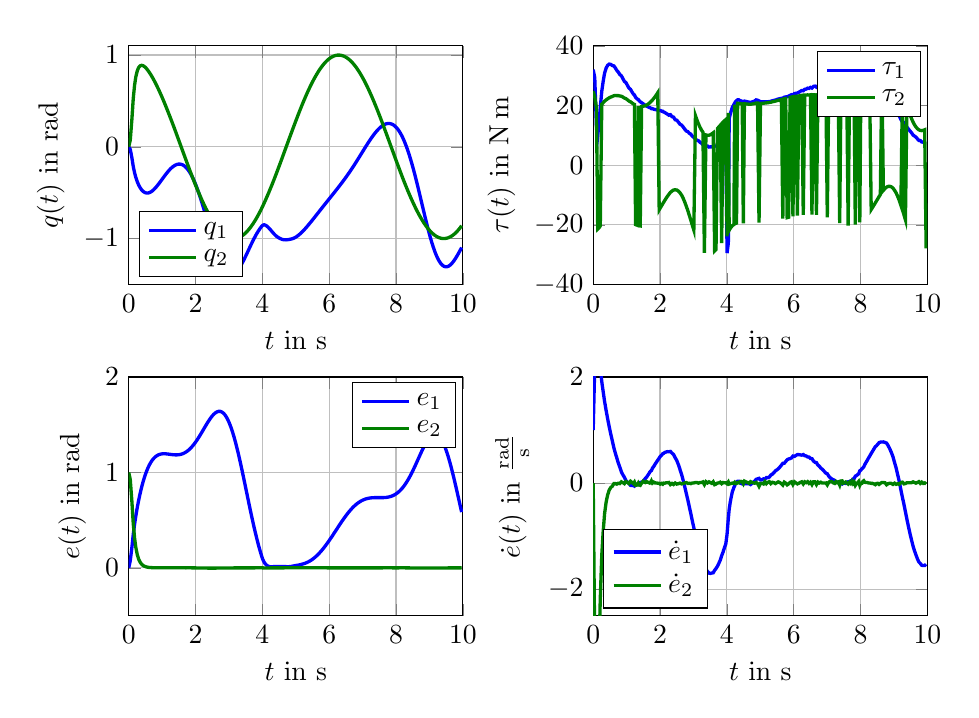
\begin{tikzpicture}

\begin{axis}[%
width=0.35\textwidth,
height=0.25\textwidth,
scale only axis,
xmin=0,
xmax=10,
xlabel={$t$ in $\mathrm{s}$},
xmajorgrids,
ymin=-1.5,
ymax=1.1,
ylabel={$q(t)$ in $\mathrm{rad}$},
ymajorgrids,
name=plot1,
legend style={at={(0.03,0.03)},anchor=south west,draw=black,fill=white,legend cell align=left}
]
\addplot [
color=blue,
solid,
line width=1.2pt
]
table[row sep=crcr]{
0 0\\
0.0464506662257798 -0.0285259559019206\\
0.0964506662257798 -0.121758225900924\\
0.135692788597378 -0.213402307230893\\
0.175110577946704 -0.281914258237024\\
0.211920567405195 -0.331950473772182\\
0.257095804732146 -0.380538838327579\\
0.297837878467808 -0.415341362396376\\
0.341045203229129 -0.444819646473483\\
0.386755411781201 -0.468758909193796\\
0.431851704569002 -0.485845383694429\\
0.47910413143125 -0.497446029043677\\
0.526208504840362 -0.50312019449801\\
0.573019131135802 -0.503455104774961\\
0.61856409127426 -0.499221708893456\\
0.665480135947291 -0.49060769337871\\
0.706699867862032 -0.480019383301941\\
0.748060022497881 -0.466850285384168\\
0.794958142802112 -0.44922727752906\\
0.842573696922153 -0.429032578625044\\
0.888450425413438 -0.40807483363465\\
0.933715852030132 -0.38631379901638\\
0.978743980749002 -0.364067702294442\\
1.02409419212842 -0.341433361577126\\
1.06977764276503 -0.318824069208732\\
1.1163558010176 -0.296423204242102\\
1.1636295164923 -0.274780325886433\\
1.20328573762012 -0.257954346554076\\
1.23388824108185 -0.246001475063806\\
1.26937874065552 -0.233128601412589\\
1.29629645176842 -0.224365745830516\\
1.32314089387168 -0.216434827709227\\
1.35019384435781 -0.209325247253921\\
1.37788774978945 -0.203030724470327\\
1.4075105830504 -0.197465417501049\\
1.4483897324819 -0.191675912143429\\
1.4916062051548 -0.18851359479294\\
1.5257637834091 -0.188277137759371\\
1.55988908497502 -0.190029453853763\\
1.59578628555792 -0.194099626700858\\
1.62541821256489 -0.199228467072192\\
1.65810672066234 -0.20675658434105\\
1.68956135131949 -0.215870265913984\\
1.7135577643755 -0.224114734615981\\
1.74356849787367 -0.235924718869769\\
1.77530153508033 -0.250315090360914\\
1.81230750533452 -0.26957037221344\\
1.85053826606999 -0.292319522329387\\
1.88560198673001 -0.315867024486181\\
1.93208075742107 -0.350507393107905\\
1.97494325771518 -0.385791019609149\\
2.00606329214472 -0.413512722834108\\
2.0459278082405 -0.451532464050077\\
2.08087759021467 -0.486810559124921\\
2.10722639856243 -0.514529358338333\\
2.13809740660548 -0.548235690141749\\
2.17892402036648 -0.594686416876999\\
2.22015024634027 -0.643433161647189\\
2.26458644414952 -0.697553513046846\\
2.31029858981492 -0.754611557576414\\
2.35843605732266 -0.815657328209612\\
2.40557806620482 -0.875525401618263\\
2.45188500537926 -0.933924825532278\\
2.50059832335924 -0.994262907596584\\
2.54811148689231 -1.05116214206552\\
2.59612253655827 -1.10608159938385\\
2.64372512719945 -1.15730885355461\\
2.69249401424562 -1.20582970877748\\
2.73937471190073 -1.24804022153371\\
2.78602419061342 -1.28530314986919\\
2.83269234618716 -1.3173942371385\\
2.87530689917059 -1.34187527289835\\
2.91945149562892 -1.36219453622427\\
2.96522265355164 -1.37765849812358\\
3.01164728326785 -1.3873701375885\\
3.05990837248807 -1.39138916026531\\
3.10464499724735 -1.38940981875817\\
3.14965759806055 -1.38227943817956\\
3.19342220260785 -1.37060929988106\\
3.23959891996394 -1.35359980075536\\
3.28384196194181 -1.33316003784053\\
3.32750148424176 -1.30945890396531\\
3.37373261361323 -1.28105236937731\\
3.41990231986215 -1.24986592622897\\
3.4655107116021 -1.21688591808501\\
3.50587295264708 -1.18642258785116\\
3.54739076815679 -1.1543055226249\\
3.59163132785837 -1.11971846136079\\
3.6342331200059 -1.08652121048754\\
3.67556549674745 -1.05488960815762\\
3.71796778961887 -1.02330902533203\\
3.75861800225977 -0.994176793616927\\
3.80101008631434 -0.965357154215078\\
3.84421026803515 -0.937909514446677\\
3.88712669974031 -0.91268245049812\\
3.92870572109286 -0.890387111000836\\
3.96800254057115 -0.871193448174794\\
4.00622599872608 -0.855824193033293\\
4.04390046565695 -0.849777828587408\\
4.0693866815133 -0.850670369228283\\
4.10345694817675 -0.856207402577117\\
4.13808726585611 -0.865131421414277\\
4.16722174894275 -0.874680145836679\\
4.18999164279903 -0.883054830146402\\
4.21078766571001 -0.891187772477127\\
4.23262637205982 -0.899974342708316\\
4.25829726711969 -0.910738484430638\\
4.28836461638695 -0.923458857901012\\
4.32245890850725 -0.938038936841001\\
4.35727104909634 -0.952022114313621\\
4.38783819584798 -0.963130168697887\\
4.42556571181493 -0.974996890943904\\
4.45941216300152 -0.98402881847217\\
4.49297192258574 -0.991562677122564\\
4.5250895993663 -0.997833061663379\\
4.55844794003427 -1.00345529312994\\
4.59498596289363 -1.0082142961357\\
4.62842105392876 -1.0111730175354\\
4.66636462312292 -1.01314334717346\\
4.70858794366504 -1.01339730528117\\
4.75054470976503 -1.01207432428161\\
4.79209411557478 -1.00980434754282\\
4.83373760467736 -1.00684049587996\\
4.87562247555478 -1.00310392346767\\
4.91853911423006 -0.998592338053697\\
4.96250002851763 -0.991665000416645\\
5.00640568839406 -0.982421211297385\\
5.05103197815631 -0.971137573970678\\
5.09522850095571 -0.958536665970621\\
5.13938513323832 -0.944648678261601\\
5.18347759850464 -0.929562268767828\\
5.22530977893891 -0.914136001240111\\
5.27037105593176 -0.896263719723375\\
5.31584840902946 -0.877456302431258\\
5.36140050464104 -0.858047220592042\\
5.40653327247306 -0.83835580129662\\
5.45300247752129 -0.817625674769284\\
5.49375289570647 -0.799293806841971\\
5.53735764340338 -0.779396712648078\\
5.58441921720224 -0.75770065240626\\
5.63102812921806 -0.736187481677271\\
5.67401964442284 -0.716383013130853\\
5.71804918356858 -0.696021061352711\\
5.76059782888716 -0.676369744599322\\
5.8042762615115 -0.656238074425145\\
5.84897454468086 -0.635678507833338\\
5.89207474601732 -0.615917642854356\\
5.93533243881451 -0.596168654787775\\
5.9771839931477 -0.577083094641146\\
6.02270486978421 -0.556396473407818\\
6.06560765741539 -0.536888242699679\\
6.11042023913344 -0.516508324466523\\
6.15517384557642 -0.496090235658145\\
6.19859629240825 -0.476178812901058\\
6.24231686902312 -0.455974384363889\\
6.28640940304939 -0.435384946991999\\
6.33013618200034 -0.414793056494242\\
6.37452084839191 -0.393568312334599\\
6.41564791812484 -0.373607894248271\\
6.4588416701997 -0.352261417196267\\
6.50230811743895 -0.33046017946765\\
6.54644279006697 -0.307896519549747\\
6.591371972071 -0.284449966504483\\
6.6361375119493 -0.260585701820867\\
6.681069026513 -0.236177584678216\\
6.72489876577292 -0.21192346128197\\
6.76695879821501 -0.188276872247144\\
6.80893712617841 -0.164261099753132\\
6.84940145306385 -0.140831383260492\\
6.88826936926153 -0.118159295447524\\
6.92628590277054 -0.0958504497717212\\
6.96496310652254 -0.0730724994258489\\
7.00557114065612 -0.0491921634217407\\
7.04512030947785 -0.025953705228542\\
7.0843415724757 -0.00307953928097519\\
7.11901408289293 0.0169220474385241\\
7.15347497656874 0.0365278801982223\\
7.19067501441045 0.0573246447029384\\
7.22747524685934 0.0774236771725574\\
7.26513104597926 0.0974157853251193\\
7.29962263496502 0.115097838463639\\
7.33662347877812 0.13329278826258\\
7.37646410496285 0.151920075015398\\
7.41042352872656 0.16689172320806\\
7.44755814368743 0.182239984928649\\
7.48361309066031 0.19601435407334\\
7.51984799660532 0.208606865637015\\
7.55573387789736 0.219782991039827\\
7.5925604288034 0.229834257519734\\
7.6292646772642 0.238273634286988\\
7.66662762848344 0.245175712691512\\
7.70375119945567 0.250129203481308\\
7.73906680485327 0.253100913246752\\
7.77503392516948 0.254262628021193\\
7.8099095314224 0.2535153666842\\
7.84365268869173 0.250938675630521\\
7.87936745713217 0.246177170087394\\
7.91277268611033 0.239745322832405\\
7.94405657291399 0.231987314382325\\
7.9779708521006 0.221584262241359\\
8.00656674263881 0.211175896828996\\
8.04020908123712 0.197018442319871\\
8.06451428214386 0.185379661582736\\
8.09745961862698 0.167881335747641\\
8.12777998278437 0.149838905107519\\
8.16128360926469 0.127848757706329\\
8.19896315215115 0.100383394734351\\
8.2383659313604 0.0686403589482551\\
8.27387216749484 0.0371357777805561\\
8.31923171233621 -0.00662006497231941\\
8.36594962163188 -0.0556386324789899\\
8.39827831661913 -0.0919452771927281\\
8.4409420473085 -0.142991134209307\\
8.47766244321635 -0.189235258099263\\
8.51651781864552 -0.240407939816876\\
8.55487987951988 -0.293010227573297\\
8.59299524704441 -0.347150270984557\\
8.63830029891275 -0.41359476668964\\
8.68370742608802 -0.48189057241859\\
8.73176596203796 -0.555391718229527\\
8.77977382959902 -0.629382671209516\\
8.8269245333688 -0.701788487405694\\
8.87475321532245 -0.774236230866394\\
8.92180087562252 -0.843635968653664\\
8.96984560348556 -0.911897601578446\\
9.0181361046177 -0.976981148915892\\
9.06546939035572 -1.03654145294981\\
9.11398242013477 -1.09258566341916\\
9.16068323615229 -1.14114577991225\\
9.20779297352458 -1.18437358658453\\
9.25359894615191 -1.2203992667926\\
9.29980520294477 -1.25052056840905\\
9.34365272832576 -1.27319508433785\\
9.38772064956589 -1.29002386392767\\
9.43706574967344 -1.3020824130568\\
9.48127332540276 -1.3069392816181\\
9.52602139485836 -1.3060799238354\\
9.5714441178355 -1.2998944706606\\
9.61513449734196 -1.28926489171669\\
9.65714436917794 -1.27510717068689\\
9.70335834238266 -1.25551413716119\\
9.7462598662786 -1.23409835146777\\
9.78917395267524 -1.21011242725444\\
9.83225347752565 -1.18400748278952\\
9.87665843113713 -1.15549426168923\\
9.91990269203068 -1.12667871870973\\
9.96311489100695 -1.09743639998989\\
};
\addlegendentry{$q_1$};

\addplot [
color=green!50!black,
solid,
line width=1.2pt
]
table[row sep=crcr]{
0 0\\
0.0464506662257798 0.0724907345297772\\
0.0964506662257798 0.305718112045594\\
0.135692788597378 0.524470659001438\\
0.175110577946704 0.67052668523728\\
0.211920567405195 0.76054248032264\\
0.257095804732146 0.828904275177569\\
0.297837878467808 0.863676563337024\\
0.341045203229129 0.882148482531038\\
0.386755411781201 0.887535195550551\\
0.431851704569002 0.883110940404232\\
0.47910413143125 0.871315730593596\\
0.526208504840362 0.854218267502579\\
0.573019131135802 0.833224927547489\\
0.61856409127426 0.80981942566324\\
0.665480135947291 0.783003852670116\\
0.706699867862032 0.757747479890531\\
0.748060022497881 0.730754252288348\\
0.794958142802112 0.698156159278691\\
0.842573696922153 0.663349389607643\\
0.888450425413438 0.62863924642222\\
0.933715852030132 0.593012184231888\\
0.978743980749002 0.556344339440604\\
1.02409419212842 0.518117822672394\\
1.06977764276503 0.478381783299125\\
1.1163558010176 0.436761371615133\\
1.1636295164923 0.393455155117454\\
1.20328573762012 0.356809775780663\\
1.23388824108185 0.328433413408057\\
1.26937874065552 0.294775690727726\\
1.29629645176842 0.269261921780837\\
1.32314089387168 0.243544431271942\\
1.35019384435781 0.217396923737013\\
1.37788774978945 0.190432305808204\\
1.4075105830504 0.161400079423959\\
1.4483897324819 0.1205467760042\\
1.4916062051548 0.077469210520449\\
1.5257637834091 0.0435410574264513\\
1.55988908497502 0.00957599459503895\\
1.59578628555792 -0.0261592414003927\\
1.62541821256489 -0.0556242327703249\\
1.65810672066234 -0.0881273212102964\\
1.68956135131949 -0.119410118048523\\
1.7135577643755 -0.143154414670417\\
1.74356849787367 -0.172903121646915\\
1.77530153508033 -0.204202148725035\\
1.81230750533452 -0.24046384285039\\
1.85053826606999 -0.277438982702339\\
1.88560198673001 -0.310440565317708\\
1.93208075742107 -0.353885858912848\\
1.97494325771518 -0.393670725448783\\
2.00606329214472 -0.421928461103697\\
2.0459278082405 -0.457108416085183\\
2.08087759021467 -0.487614856172259\\
2.10722639856243 -0.510412517381599\\
2.13809740660548 -0.536638322187593\\
2.17892402036648 -0.570396600142427\\
2.22015024634027 -0.603474521206264\\
2.26458644414952 -0.638223053693621\\
2.31029858981492 -0.672572199602029\\
2.35843605732266 -0.706964938320139\\
2.40557806620482 -0.739406916605953\\
2.45188500537926 -0.769693025394074\\
2.50059832335924 -0.799565457632889\\
2.54811148689231 -0.827117979839644\\
2.59612253655827 -0.85308700140732\\
2.64372512719945 -0.876954064633234\\
2.69249401424562 -0.899235488028603\\
2.73937471190073 -0.918768860303051\\
2.78602419061342 -0.936131111672048\\
2.83269234618716 -0.951416382816907\\
2.87530689917059 -0.963612646576002\\
2.91945149562892 -0.974359929586596\\
2.96522265355164 -0.983538293909349\\
3.01164728326785 -0.991092805155318\\
3.05990837248807 -0.99625180718512\\
3.10464499724735 -0.999272827290216\\
3.14965759806055 -1.00020258286706\\
3.19342220260785 -0.999124030856312\\
3.23959891996394 -0.995828178523382\\
3.28384196194181 -0.990633390330167\\
3.32750148424176 -0.983546200914704\\
3.37373261361323 -0.973954703394232\\
3.41990231986215 -0.962286458589955\\
3.4655107116021 -0.948807444807337\\
3.50587295264708 -0.935223379886899\\
3.54739076815679 -0.919650127242089\\
3.59163132785837 -0.901283114246839\\
3.6342331200059 -0.881941961860439\\
3.67556549674745 -0.861504853649544\\
3.71796778961887 -0.83914663708117\\
3.75861800225977 -0.816442712134963\\
3.80101008631434 -0.791300470576417\\
3.84421026803515 -0.76410672181325\\
3.88712669974031 -0.735796865408588\\
3.92870572109286 -0.707027169500211\\
3.96800254057115 -0.678667875124702\\
4.00622599872608 -0.649713433698121\\
4.04390046565695 -0.619753461516711\\
4.0693866815133 -0.599390105960675\\
4.10345694817675 -0.571615429727356\\
4.13808726585611 -0.542914394655913\\
4.16722174894275 -0.518453348693432\\
4.18999164279903 -0.498956842529176\\
4.21078766571001 -0.48091470547058\\
4.23262637205982 -0.461733025152952\\
4.25829726711969 -0.438929795754505\\
4.28836461638695 -0.411889734618235\\
4.32245890850725 -0.380770182659032\\
4.35727104909634 -0.348447689742336\\
4.38783819584798 -0.319657689183067\\
4.42556571181493 -0.283731347224832\\
4.45941216300152 -0.250999328654139\\
4.49297192258574 -0.218347879300581\\
4.5250895993663 -0.186949981290107\\
4.55844794003427 -0.154126325702428\\
4.59498596289363 -0.117984709060116\\
4.62842105392876 -0.0847449373854493\\
4.66636462312292 -0.0469180255950904\\
4.70858794366504 -0.004813174922733\\
4.75054470976503 0.0368817564175765\\
4.79209411557478 0.0781469549631466\\
4.83373760467736 0.119330623892362\\
4.87562247555478 0.160634046224372\\
4.91853911423006 0.202647510123685\\
4.96250002851763 0.245305305358293\\
5.00640568839406 0.2875589942782\\
5.05103197815631 0.330111600826617\\
5.09522850095571 0.371615750199133\\
5.13938513323832 0.412322137136344\\
5.18347759850464 0.452111046766828\\
5.22530977893891 0.4891506501317\\
5.27037105593176 0.527845354144517\\
5.31584840902946 0.565862470009048\\
5.36140050464104 0.602788908155086\\
5.40653327247306 0.638168749427391\\
5.45300247752129 0.673084825844491\\
5.49375289570647 0.702780698996458\\
5.53735764340338 0.733061148419346\\
5.58441921720224 0.764035694903183\\
5.63102812921806 0.79324853905965\\
5.67401964442284 0.818870520025202\\
5.71804918356858 0.843344568978551\\
5.76059782888716 0.86544718962502\\
5.8042762615115 0.886491948521011\\
5.84897454468086 0.906220479354346\\
5.89207474601732 0.923522012793574\\
5.93533243881451 0.939214687564591\\
5.9771839931477 0.952645183660125\\
6.02270486978421 0.965443352670057\\
6.06560765741539 0.975604882348742\\
6.11042023913344 0.984343515837903\\
6.15517384557642 0.991069328868045\\
6.19859629240825 0.995687856149877\\
6.24231686902312 0.998412586657729\\
6.28640940304939 0.999173503960426\\
6.33013618200034 0.998170114068525\\
6.37452084839191 0.995102468642053\\
6.41564791812484 0.990513203631012\\
6.4588416701997 0.983819443264451\\
6.50230811743895 0.975407162468312\\
6.54644279006697 0.964956031541295\\
6.591371972071 0.952336417123071\\
6.6361375119493 0.937772562054957\\
6.681069026513 0.921315086280733\\
6.72489876577292 0.903460991988664\\
6.76695879821501 0.88471937119181\\
6.80893712617841 0.864270601327965\\
6.84940145306385 0.843125977860776\\
6.88826936926153 0.821621922203234\\
6.92628590277054 0.799397884940896\\
6.96496310652254 0.775600904757281\\
7.00557114065612 0.749468755302913\\
7.04512030947785 0.722679592138656\\
7.0843415724757 0.695030879378195\\
7.11901408289293 0.669726878996863\\
7.15347497656874 0.643793258179047\\
7.19067501441045 0.614903804157597\\
7.22747524685934 0.585483271352624\\
7.26513104597926 0.554518908267069\\
7.29962263496502 0.525515107034288\\
7.33662347877812 0.493772779393363\\
7.37646410496285 0.458797037881455\\
7.41042352872656 0.428428296575183\\
7.44755814368743 0.39460418762617\\
7.48361309066031 0.361211501652009\\
7.51984799660532 0.32722791004471\\
7.55573387789736 0.293103910156011\\
7.5925604288034 0.257592822251305\\
7.6292646772642 0.221875484527215\\
7.66662762848344 0.185154585483309\\
7.70375119945567 0.148632991707926\\
7.73906680485327 0.113622392020462\\
7.77503392516948 0.0778264905900226\\
7.8099095314224 0.0430149726676655\\
7.84365268869173 0.00934382866158592\\
7.87936745713217 -0.0263058868866601\\
7.91277268611033 -0.0595703294123992\\
7.94405657291399 -0.0907482705015097\\
7.9779708521006 -0.124427705385886\\
8.00656674263881 -0.152731497289388\\
8.04020908123712 -0.186006109477481\\
8.06451428214386 -0.20975362299698\\
8.09745961862698 -0.242012617017272\\
8.12777998278437 -0.271339499958929\\
8.16128360926469 -0.303631509197552\\
8.19896315215115 -0.339414645616246\\
8.2383659313604 -0.376369823830403\\
8.27387216749484 -0.408530813147513\\
8.31923171233621 -0.449056368743283\\
8.36594962163188 -0.49028510557386\\
8.39827831661913 -0.518209494978234\\
8.4409420473085 -0.553477972312195\\
8.47766244321635 -0.583376310984448\\
8.51651781864552 -0.614327779161763\\
8.55487987951988 -0.644106239512928\\
8.59299524704441 -0.672711951780415\\
8.63830029891275 -0.705271410392011\\
8.68370742608802 -0.736486904500404\\
8.73176596203796 -0.767962919123919\\
8.77977382959902 -0.797564161741147\\
8.8269245333688 -0.824987383043374\\
8.87475321532245 -0.850848133008793\\
8.92180087562252 -0.874582651001303\\
8.96984560348556 -0.896712299718648\\
9.0181361046177 -0.916800266158033\\
9.06546939035572 -0.934577062708971\\
9.11398242013477 -0.950627625425005\\
9.16068323615229 -0.964080550104835\\
9.20779297352458 -0.975360777504356\\
9.25359894615191 -0.984346261575102\\
9.29980520294477 -0.991275988392843\\
9.34365272832576 -0.995877907113643\\
9.38772064956589 -0.998862296434441\\
9.43706574967344 -0.99966963530417\\
9.48127332540276 -0.998002989315693\\
9.52602139485836 -0.994884952832985\\
9.5714441178355 -0.989562574900921\\
9.61513449734196 -0.982407298077207\\
9.65714436917794 -0.973654309255679\\
9.70335834238266 -0.962098794347427\\
9.7462598662786 -0.94954825319523\\
9.78917395267524 -0.935203454772355\\
9.83225347752565 -0.918965385818368\\
9.87665843113713 -0.900430869810098\\
9.91990269203068 -0.880735949598875\\
9.96311489100695 -0.859292233526438\\
};
\addlegendentry{$q_2$};

\end{axis}

\begin{axis}[%
width=0.35\textwidth,
height=0.25\textwidth,
scale only axis,
xmin=0,
xmax=10,
xlabel={$t$ in $\mathrm{s}$},
xmajorgrids,
ymin=-0.5,
ymax=2,
ylabel={$e(t)$ in $\mathrm{rad}$},
ymajorgrids,
name=plot3,
at=(plot1.below south west),
anchor=above north west,
legend style={draw=black,fill=white,legend cell align=left}
]
\addplot [
color=blue,
solid,
line width=1.2pt
]
table[row sep=crcr]{
0 0\\
0.0464506662257798 0.0749599197716165\\
0.0964506662257798 0.218059419234925\\
0.135692788597378 0.348679071027998\\
0.175110577946704 0.456131283804683\\
0.211920567405195 0.542288362299316\\
0.257095804732146 0.634811724810686\\
0.297837878467808 0.708795326329261\\
0.341045203229129 0.779291926496638\\
0.386755411781201 0.845944379356207\\
0.431851704569002 0.904398606508376\\
0.47910413143125 0.958430388512027\\
0.526208504840362 1.00537858108246\\
0.573019131135802 1.04562649968238\\
0.61856409127426 1.07908761565586\\
0.665480135947291 1.10804458200286\\
0.706699867862032 1.12934691495116\\
0.748060022497881 1.14706830367603\\
0.794958142802112 1.16306156988072\\
0.842573696922153 1.17539107749462\\
0.888450425413438 1.18417032772601\\
0.933715852030132 1.19014966320489\\
0.978743980749002 1.19386478683864\\
1.02409419212842 1.1956769966164\\
1.06977764276503 1.19591779270269\\
1.1163558010176 1.19492995966129\\
1.1636295164923 1.19302680218813\\
1.20328573762012 1.19117901170893\\
1.23388824108185 1.18978274612138\\
1.26937874065552 1.18804520543135\\
1.29629645176842 1.18692663049445\\
1.32314089387168 1.18592464101394\\
1.35019384435781 1.18509103995922\\
1.37788774978945 1.1844814959362\\
1.4075105830504 1.18416389391449\\
1.4483897324819 1.18419357453653\\
1.4916062051548 1.18537969536719\\
1.5257637834091 1.18726334412006\\
1.55988908497502 1.18996997048143\\
1.59578628555792 1.19378739393094\\
1.62541821256489 1.19773706273165\\
1.65810672066234 1.20294745260922\\
1.68956135131949 1.20882598627227\\
1.7135577643755 1.21394161625525\\
1.74356849787367 1.22103669689114\\
1.77530153508033 1.2294766783741\\
1.81230750533452 1.24054802699141\\
1.85053826606999 1.25344624517746\\
1.88560198673001 1.26672359519811\\
1.93208075742107 1.28595097309281\\
1.97494325771518 1.30522920752773\\
2.00606329214472 1.32027023084302\\
2.0459278082405 1.34076504646649\\
2.08087759021467 1.35951539293649\\
2.10722639856243 1.37406799891539\\
2.13809740660548 1.39159002109393\\
2.17892402036648 1.41540558087349\\
2.22015024634027 1.43990779312657\\
2.26458644414952 1.46638144373494\\
2.31029858981492 1.49341564284604\\
2.35843605732266 1.52117730693336\\
2.40557806620482 1.54686486410422\\
2.45188500537926 1.57023650540257\\
2.50059832335924 1.59225560166608\\
2.54811148689231 1.61041243102242\\
2.59612253655827 1.62490164248928\\
2.64372512719945 1.63486188184374\\
2.69249401424562 1.63998343871382\\
2.73937471190073 1.63950046391855\\
2.78602419061342 1.63342647622815\\
2.83269234618716 1.62140541515868\\
2.87530689917059 1.60502519616442\\
2.91945149562892 1.58251320805823\\
2.96522265355164 1.55311554729926\\
3.01164728326785 1.51695011130775\\
3.05990837248807 1.4729826343657\\
3.10464499724735 1.42634906928629\\
3.14965759806055 1.37421458113698\\
3.19342220260785 1.31880295271792\\
3.23959891996394 1.25575035447402\\
3.28384196194181 1.19138997696507\\
3.32750148424176 1.12461912393419\\
3.37373261361323 1.05099176227416\\
3.41990231986215 0.975135176118242\\
3.4655107116021 0.898602622029715\\
3.50587295264708 0.830145675512142\\
3.54739076815679 0.759553338812632\\
3.59163132785837 0.684718103441778\\
3.6342331200059 0.613567195358306\\
3.67556549674745 0.545932468336528\\
3.71796778961887 0.478320745637177\\
3.75861800225977 0.41556520480041\\
3.80101008631434 0.352700629878762\\
3.84421026803515 0.291691974595514\\
3.88712669974031 0.234318165877081\\
3.92870572109286 0.182068749850014\\
3.96800254057115 0.135689707673275\\
4.00622599872608 0.094966807609034\\
4.04390046565695 0.0650184472447705\\
4.0693866815133 0.0503711828120882\\
4.10345694817675 0.0359480482782905\\
4.13808726585611 0.0255595716874649\\
4.16722174894275 0.0196395628179458\\
4.18999164279903 0.0164293325337008\\
4.21078766571001 0.0143740465612145\\
4.23262637205982 0.0128698223912522\\
4.25829726711969 0.0120786690426175\\
4.28836461638695 0.012018283604832\\
4.32245890850725 0.0131032933829983\\
4.35727104909634 0.0144166237940621\\
4.38783819584798 0.0153360994590901\\
4.42556571181493 0.015849458651729\\
4.45941216300152 0.0158571650577062\\
4.49297192258574 0.0155381783578679\\
4.5250895993663 0.0153223722940909\\
4.55844794003427 0.0152808340662162\\
4.59498596289363 0.0150981180296281\\
4.62842105392876 0.0146962530613313\\
4.66636462312292 0.0142022809612155\\
4.70858794366504 0.0134045292125421\\
4.75054470976503 0.0128021658145231\\
4.79209411557478 0.0129791205430874\\
4.83373760467736 0.0141942096218525\\
4.87562247555478 0.0163969548144411\\
4.91853911423006 0.0197661305176995\\
4.96250002851763 0.0227800584278631\\
5.00640568839406 0.0253336494047793\\
5.05103197815631 0.0279312338740842\\
5.09522850095571 0.0309290091337535\\
5.13938513323832 0.0344348151398658\\
5.18347759850464 0.0384875289856799\\
5.22530977893891 0.0428210816809631\\
5.27037105593176 0.0479384408384872\\
5.31584840902946 0.054078962629487\\
5.36140050464104 0.0613655989784025\\
5.40653327247306 0.0697543978826097\\
5.45300247752129 0.0795709286887042\\
5.49375289570647 0.0893401433513233\\
5.53735764340338 0.100816728847294\\
5.58441921720224 0.114427201791312\\
5.63102812921806 0.129285190939092\\
5.67401964442284 0.144199615210524\\
5.71804918356858 0.160490281852305\\
5.76059782888716 0.177245809288244\\
5.8042762615115 0.195426844445561\\
5.84897454468086 0.214983973485935\\
5.89207474601732 0.234702294313759\\
5.93533243881451 0.255288593060328\\
5.9771839931477 0.27583496979504\\
6.02270486978421 0.298851661319187\\
6.06560765741539 0.321023222984915\\
6.11042023913344 0.344601416676405\\
6.15517384557642 0.368428106942545\\
6.19859629240825 0.391690638695308\\
6.24231686902312 0.415117321867431\\
6.28640940304939 0.438609037276174\\
6.33013618200034 0.461726683584874\\
6.37452084839191 0.484776916900817\\
6.41564791812484 0.505683472492398\\
6.4588416701997 0.527015855324548\\
6.50230811743895 0.547833671468157\\
6.54644279006697 0.568123700726184\\
6.591371972071 0.587781202452598\\
6.6361375119493 0.606255231587327\\
6.681069026513 0.623645832834779\\
6.72489876577292 0.639412554835296\\
6.76695879821501 0.653399819547826\\
6.80893712617841 0.66612452969433\\
6.84940145306385 0.677273946025942\\
6.88826936926153 0.686990510935516\\
6.92628590277054 0.695529991095173\\
6.96496310652254 0.703246897312551\\
7.00557114065612 0.710368640293705\\
7.04512030947785 0.716276419069378\\
7.0843415724757 0.721240728256224\\
7.11901408289293 0.724930465401173\\
7.15347497656874 0.727987811269927\\
7.19067501441045 0.730635927532953\\
7.22747524685934 0.732657139553485\\
7.26513104597926 0.734163832775228\\
7.29962263496502 0.735140198355944\\
7.33662347877812 0.735836041695805\\
7.37646410496285 0.736218466869128\\
7.41042352872656 0.736338678640679\\
7.44755814368743 0.736300599348505\\
7.48361309066031 0.736179657269665\\
7.51984799660532 0.736087922853238\\
7.55573387789736 0.736069854694498\\
7.5925604288034 0.736189380559301\\
7.6292646772642 0.736583582492722\\
7.66662762848344 0.737324803797013\\
7.70375119945567 0.738607412498984\\
7.73906680485327 0.740303640540658\\
7.77503392516948 0.742622619907155\\
7.8099095314224 0.745513615390791\\
7.84365268869173 0.749007981288406\\
7.87936745713217 0.753500627207827\\
7.91277268611033 0.758526980980325\\
7.94405657291399 0.763958680429956\\
7.9779708521006 0.770738917072938\\
8.00656674263881 0.777205563854966\\
8.04020908123712 0.785691283239057\\
8.06451428214386 0.792540078622058\\
8.09745961862698 0.802624039855181\\
8.12777998278437 0.812911902287809\\
8.16128360926469 0.825304400743342\\
8.19896315215115 0.840698308202678\\
8.2383659313604 0.858389130782691\\
8.27387216749484 0.875997793162266\\
8.31923171233621 0.900329461791227\\
8.36594962163188 0.927420723889934\\
8.39827831661913 0.947436968886966\\
8.4409420473085 0.975619079688441\\
8.47766244321635 1.00096952665072\\
8.51651781864552 1.02884265471415\\
8.55487987951988 1.05727344071322\\
8.59299524704441 1.08628357913958\\
8.63830029891275 1.12146445640699\\
8.68370742608802 1.156968653717\\
8.73176596203796 1.19424900158399\\
8.77977382959902 1.23058441093569\\
8.8269245333688 1.26465801847306\\
8.87475321532245 1.29694455573734\\
8.92180087562252 1.32567201682737\\
8.96984560348556 1.35129915356318\\
9.0181361046177 1.37250841145709\\
9.06546939035572 1.38816849531608\\
9.11398242013477 1.39840182330173\\
9.16068323615229 1.40218126637744\\
9.20779297352458 1.39965987897987\\
9.25359894615191 1.39074351684922\\
9.29980520294477 1.37516827212514\\
9.34365272832576 1.3542313610982\\
9.38772064956589 1.32707269425652\\
9.43706574967344 1.28979493337211\\
9.48127332540276 1.25047396514519\\
9.52602139485836 1.20500936258723\\
9.5714441178355 1.15375357001702\\
9.61513449734196 1.10005588832707\\
9.65714436917794 1.04482619528196\\
9.70335834238266 0.980523098581681\\
9.7462598662786 0.918125459571833\\
9.78917395267524 0.853727416168048\\
9.83225347752565 0.787714678666648\\
9.87665843113713 0.718836233537791\\
9.91990269203068 0.651537311527221\\
9.96311489100695 0.584727548050949\\
};
\addlegendentry{$e_1$};

\addplot [
color=green!50!black,
solid,
line width=1.2pt
]
table[row sep=crcr]{
0 1\\
0.0464506662257798 0.926430627239681\\
0.0964506662257798 0.689634127195594\\
0.135692788597378 0.466337191783255\\
0.175110577946704 0.31418059512697\\
0.211920567405195 0.217086269587032\\
0.257095804732146 0.13822823859681\\
0.297837878467808 0.092296642904697\\
0.341045203229129 0.0602571063191729\\
0.386755411781201 0.0386025485773733\\
0.431851704569002 0.0250813298073455\\
0.47910413143125 0.0160925296370347\\
0.526208504840362 0.0104993240298155\\
0.573019131135802 0.00704299314455969\\
0.61856409127426 0.0048925051286296\\
0.665480135947291 0.0036165694943\\
0.706699867862032 0.00276140016435233\\
0.748060022497881 0.00225560275528824\\
0.794958142802112 0.00215848647905914\\
0.842573696922153 0.00219474203589209\\
0.888450425413438 0.00197615463541601\\
0.933715852030132 0.00183897651700382\\
0.978743980749002 0.00172088836161488\\
1.02409419212842 0.00175505793871711\\
1.06977764276503 0.001937485737115\\
1.1163558010176 0.00219831954805833\\
1.1636295164923 0.00255419926640194\\
1.20328573762012 0.00248359229981315\\
1.23388824108185 0.00213717270169766\\
1.26937874065552 0.00209849031412301\\
1.29629645176842 0.00180364835852642\\
1.32314089387168 0.00158716991076613\\
1.35019384435781 0.00142062077485902\\
1.37788774978945 0.00128202122302187\\
1.4075105830504 0.00116103721652\\
1.4483897324819 0.00155436992712692\\
1.4916062051548 0.00163816919778399\\
1.5257637834091 0.00147626702855772\\
1.55988908497502 0.00133103095747393\\
1.59578628555792 0.00117188358619043\\
1.62541821256489 0.0010295041403478\\
1.65810672066234 0.000927814450769823\\
1.68956135131949 0.0009240960553734\\
1.7135577643755 0.000877415881844396\\
1.74356849787367 0.000989216569939166\\
1.77530153508033 0.00111944498222721\\
1.81230750533452 0.00129362329562774\\
1.85053826606999 0.00133135400055301\\
1.88560198673001 0.000808877769494509\\
1.93208075742107 0.000409822009306837\\
1.97494325771518 0.000436166188026499\\
2.00606329214472 0.000275971878902437\\
2.0459278082405 -0.00034695263294493\\
2.08087759021467 -0.000633311301949047\\
2.10722639856243 -0.000658246167778875\\
2.13809740660548 -0.000719540380913819\\
2.17892402036648 -0.000935224499692744\\
2.22015024634027 -0.00119742407463763\\
2.26458644414952 -0.00123266251654941\\
2.31029858981492 -0.00134806540631194\\
2.35843605732266 -0.00172509238555474\\
2.40557806620482 -0.00174308582882476\\
2.45188500537926 -0.00173904942563596\\
2.50059832335924 -0.00193609435531683\\
2.54811148689231 -0.00188088282641463\\
2.59612253655827 -0.00179647771254277\\
2.64372512719945 -0.00164886341326342\\
2.69249401424562 -0.00160330930550812\\
2.73937471190073 -0.00142616176129418\\
2.78602419061342 -0.00131763340406266\\
2.83269234618716 -0.00125208188567905\\
2.87530689917059 -0.0011423056709734\\
2.91945149562892 -0.00106801897819575\\
2.96522265355164 -0.000948792798527776\\
3.01164728326785 -0.000476168951334399\\
3.05990837248807 -0.000413886507719452\\
3.10464499724735 -4.46857007357915e-05\\
3.14965759806055 0.000235104355438387\\
3.19342220260785 0.000466881283140208\\
3.23959891996394 0.000626949694542023\\
3.28384196194181 0.000733774288534605\\
3.32750148424176 0.000777532448901552\\
3.37373261361323 0.000778400220273756\\
3.41990231986215 0.000765260205023988\\
3.4655107116021 0.000811799536653557\\
3.50587295264708 0.000842963924440165\\
3.54739076815679 0.000862494883312359\\
3.59163132785837 0.000852834541445358\\
3.6342331200059 0.000854849496892296\\
3.67556549674745 0.000712991568395105\\
3.71796778961887 0.000702974695173886\\
3.75861800225977 0.00083948182795579\\
3.80101008631434 0.00095119134087196\\
3.84421026803515 0.000953466438740391\\
3.88712669974031 0.0010711360710437\\
3.92870572109286 0.0011340478049976\\
3.96800254057115 0.00114721292444497\\
4.00622599872608 0.000794302337856378\\
4.04390046565695 -4.70817185470596e-05\\
4.0693866815133 -0.000210771474954075\\
4.10345694817675 -0.000376346162186181\\
4.13808726585611 -0.000334267695223711\\
4.16722174894275 -0.00010773873116865\\
4.18999164279903 -2.32101784092276e-06\\
4.21078766571001 8.4496305790327e-05\\
4.23262637205982 0.000164427831782221\\
4.25829726711969 0.000283541687781219\\
4.28836461638695 0.000457991158096638\\
4.32245890850725 0.00064644561945898\\
4.35727104909634 0.000746749065471064\\
4.38783819584798 0.000774634889236736\\
4.42556571181493 0.000824643296970129\\
4.45941216300152 0.000712194496780338\\
4.49297192258574 0.0006871850741694\\
4.5250895993663 0.000743791073225808\\
4.55844794003427 0.000792577120714316\\
4.59498596289363 0.000851209223456412\\
4.62842105392876 0.000875647038584185\\
4.66636462312292 0.000909915062796925\\
4.70858794366504 0.0010121473558961\\
4.75054470976503 0.00126471540532114\\
4.79209411557478 0.00147381379053463\\
4.83373760467736 0.00172039996945761\\
4.87562247555478 0.00187551660547441\\
4.91853911423006 0.00204556606771025\\
4.96250002851763 0.00220624828596752\\
5.00640568839406 0.00223989956107534\\
5.05103197815631 0.00209586447419435\\
5.09522850095571 0.00194018266449669\\
5.13938513323832 0.00181639449408327\\
5.18347759850464 0.00174554745889977\\
5.22530977893891 0.00157362168867309\\
5.27037105593176 0.0016300666304967\\
5.31584840902946 0.0016318086413708\\
5.36140050464104 0.001610292525277\\
5.40653327247306 0.00155922609815495\\
5.45300247752129 0.00165600720767445\\
5.49375289570647 0.00146769162733906\\
5.53735764340338 0.0014653695396234\\
5.58441921720224 0.00160081659162459\\
5.63102812921806 0.00152791347071446\\
5.67401964442284 0.00125517713612133\\
5.71804918356858 0.00117114088579962\\
5.76059782888716 0.00108341987448479\\
5.8042762615115 0.00100622630793068\\
5.84897454468086 0.000981873359877428\\
5.89207474601732 0.00096425429592184\\
5.93533243881451 0.000892106111899493\\
5.9771839931477 0.000900603010187573\\
6.02270486978421 0.000823002827344932\\
6.06560765741539 0.000818331869121502\\
6.11042023913344 0.000769683268696864\\
6.15517384557642 0.000748386688499414\\
6.19859629240825 0.000736625895490062\\
6.24231686902312 0.000752414953196667\\
6.28640940304939 0.000821298646987656\\
6.33013618200034 0.000727896064700473\\
6.37452084839191 0.000729339673529728\\
6.41564791812484 0.000726445309384149\\
6.4588416701997 0.000792605389469014\\
6.50230811743895 0.000681340166313826\\
6.54644279006697 0.000591385304177905\\
6.591371972071 0.000548760271450344\\
6.6361375119493 0.000583754165611183\\
6.681069026513 0.000567963064726618\\
6.72489876577292 0.000559513803630285\\
6.76695879821501 0.000526721086674287\\
6.80893712617841 0.000676274316809389\\
6.84940145306385 0.000810854404314942\\
6.88826936926153 0.000832361198860765\\
6.92628590277054 0.000842358809751032\\
6.96496310652254 0.000852717971168149\\
7.00557114065612 0.000761653592365907\\
7.04512030947785 0.000821997877166858\\
7.0843415724757 0.000845910470164135\\
7.11901408289293 0.000836204682387987\\
7.15347497656874 0.000811859314583829\\
7.19067501441045 0.000821894998843109\\
7.22747524685934 0.000834961668035317\\
7.26513104597926 0.000886654146632582\\
7.29962263496502 0.000883297926424609\\
7.33662347877812 0.000812983579215443\\
7.37646410496285 0.000778777865226288\\
7.41042352872656 0.000727667121192821\\
7.44755814368743 0.000722506433042558\\
7.48361309066031 0.000747508756956006\\
7.51984799660532 0.00072293474663454\\
7.55573387789736 0.0007418611281656\\
7.5925604288034 0.000860907984003234\\
7.6292646772642 0.000954959740431999\\
7.66662762848344 0.00110527358402054\\
7.70375119945567 0.0010329837836309\\
7.73906680485327 0.00103968765035341\\
7.77503392516948 0.00103923366859779\\
7.8099095314224 0.00104286402691726\\
7.84365268869173 0.000984932961259788\\
7.87936745713217 0.000922790247841195\\
7.91277268611033 0.000813138870087451\\
7.94405657291399 0.000795085914325339\\
7.9779708521006 0.000755930936066657\\
8.00656674263881 0.000737786313450395\\
8.04020908123712 0.000853212411582482\\
8.06451428214386 0.000772806370693352\\
8.09745961862698 0.000933136500938792\\
8.12777998278437 0.000949258160812316\\
8.16128360926469 0.00114339945203229\\
8.19896315215115 0.00123536121647405\\
8.2383659313604 0.00138139044987556\\
8.27387216749484 0.000870315162719737\\
8.31923171233621 0.00041005588917753\\
8.36594962163188 0.000391254729454116\\
8.39827831661913 0.000392958507901553\\
8.4409420473085 -0.000354768149396723\\
8.47766244321635 -0.00065063810200805\\
8.51651781864552 -0.000790664997458834\\
8.55487987951988 -0.000798203828125788\\
8.59299524704441 -0.000847216203970103\\
8.63830029891275 -0.00107163826031276\\
8.68370742608802 -0.00125938261356917\\
8.73176596203796 -0.00136235116489447\\
8.77977382959902 -0.00153312154181806\\
8.8269245333688 -0.00155837551812565\\
8.87475321532245 -0.00166345466061379\\
8.92180087562252 -0.00156873332738339\\
8.96984560348556 -0.00157845282944036\\
9.0181361046177 -0.00165397036476012\\
9.06546939035572 -0.00156311006257936\\
9.11398242013477 -0.00146295658632556\\
9.16068323615229 -0.00124865529914719\\
9.20779297352458 -0.00119020032868578\\
9.25359894615191 -0.00103835189957902\\
9.29980520294477 -0.000925074879266741\\
9.34365272832576 -0.000833245552373185\\
9.38772064956589 -0.000451159980144111\\
9.43706574967344 -0.000254870767662396\\
9.48127332540276 -0.000401571989799843\\
9.52602139485836 5.692998415463e-06\\
9.5714441178355 0.000298789473047623\\
9.61513449734196 0.00047046047699395\\
9.65714436917794 0.000530127885924436\\
9.70335834238266 0.000652005023668467\\
9.7462598662786 0.000780035142517232\\
9.78917395267524 0.000864263753938332\\
9.83225347752565 0.000841203912440469\\
9.87665843113713 0.000803298839253896\\
9.91990269203068 0.000826497904765633\\
9.96311489100695 0.000729694660774216\\
};
\addlegendentry{$e_2$};

\end{axis}

\begin{axis}[%
width=0.35\textwidth,
height=0.25\textwidth,
scale only axis,
xmin=0,
xmax=10,
xlabel={$t$ in $\mathrm{s}$},
xmajorgrids,
ymin=-2.5,
ymax=2,
ylabel={$\dot{e}(t)$ in $\mathrm{\frac{rad}{s}}$},
ymajorgrids,
name=plot2,
at=(plot3.right of south east),
anchor=left of south west,
legend style={at={(0.03,0.03)},anchor=south west,draw=black,fill=white,legend cell align=left}
]
\addplot [
color=blue,
solid,
line width=1.2pt
]
table[row sep=crcr]{
0 1\\
0.0464506662257798 2.21373012574298\\
0.0964506662257798 3.5183211554358\\
0.135692788597378 2.98598496075295\\
0.175110577946704 2.51021996745309\\
0.211920567405195 2.19533762988478\\
0.257095804732146 1.91033254633268\\
0.297837878467808 1.72550628303567\\
0.341045203229129 1.5385427064797\\
0.386755411781201 1.36983591573165\\
0.431851704569002 1.21482259731654\\
0.47910413143125 1.06222598957514\\
0.526208504840362 0.923173059375931\\
0.573019131135802 0.794702278748655\\
0.61856409127426 0.665643020128299\\
0.665480135947291 0.557479589343299\\
0.706699867862032 0.473058377327786\\
0.748060022497881 0.384869419725588\\
0.794958142802112 0.302412389629156\\
0.842573696922153 0.212786772529469\\
0.888450425413438 0.155609863164236\\
0.933715852030132 0.109041434642667\\
0.978743980749002 0.0480119139754698\\
1.02409419212842 0.0175144007023751\\
1.06977764276503 -0.00374902543314154\\
1.1163558010176 -0.0429356569931984\\
1.1636295164923 -0.0475903235208504\\
1.20328573762012 -0.0455471573982854\\
1.23388824108185 -0.057409233351259\\
1.26937874065552 -0.0311733887424493\\
1.29629645176842 -0.0277806664461525\\
1.32314089387168 -0.0227531391396222\\
1.35019384435781 -0.0279617761006673\\
1.37788774978945 -0.00433558872855908\\
1.4075105830504 0.0114126375983911\\
1.4483897324819 0.0160728338898082\\
1.4916062051548 0.0279544814220728\\
1.5257637834091 0.0578507883375225\\
1.55988908497502 0.0866524184638518\\
1.59578628555792 0.107481138194325\\
1.62541821256489 0.138340574640159\\
1.65810672066234 0.167255763005221\\
1.68956135131949 0.201391110080753\\
1.7135577643755 0.223285560767217\\
1.74356849787367 0.236116354798316\\
1.77530153508033 0.283098725843137\\
1.81230750533452 0.312007064920754\\
1.85053826606999 0.355104409592543\\
1.88560198673001 0.387979970350485\\
1.93208075742107 0.43249366466133\\
1.97494325771518 0.470520646645666\\
2.00606329214472 0.501368260288364\\
2.0459278082405 0.524435919221891\\
2.08087759021467 0.552726860404714\\
2.10722639856243 0.559917076243445\\
2.13809740660548 0.575248753932331\\
2.17892402036648 0.585488746828534\\
2.22015024634027 0.592118636189713\\
2.26458644414952 0.590354423134597\\
2.31029858981492 0.595579697554503\\
2.35843605732266 0.563910418174305\\
2.40557806620482 0.537295955979289\\
2.45188500537926 0.480113382226182\\
2.50059832335924 0.425707042451053\\
2.54811148689231 0.349900054487584\\
2.59612253655827 0.258475936183397\\
2.64372512719945 0.166444855223637\\
2.69249401424562 0.0524131251581852\\
2.73937471190073 -0.0691810651579191\\
2.78602419061342 -0.195316184100698\\
2.83269234618716 -0.319713058308738\\
2.87530689917059 -0.443987648433747\\
2.91945149562892 -0.569826083256055\\
2.96522265355164 -0.708932834870558\\
3.01164728326785 -0.842676757766471\\
3.05990837248807 -0.982348165407401\\
3.10464499724735 -1.102085615685\\
3.14965759806055 -1.21151474120399\\
3.19342220260785 -1.31775745741618\\
3.23959891996394 -1.41550112882266\\
3.28384196194181 -1.50192853532119\\
3.32750148424176 -1.55121086837256\\
3.37373261361323 -1.62999092619364\\
3.41990231986215 -1.66412688578458\\
3.4655107116021 -1.69828110555254\\
3.50587295264708 -1.70307323349643\\
3.54739076815679 -1.6962274359533\\
3.59163132785837 -1.69228740534393\\
3.6342331200059 -1.6439738423401\\
3.67556549674745 -1.61083115639544\\
3.71796778961887 -1.56919765501682\\
3.75861800225977 -1.5153126793875\\
3.80101008631434 -1.4550860664058\\
3.84421026803515 -1.37004954885848\\
3.88712669974031 -1.30003682713562\\
3.92870572109286 -1.21725149006176\\
3.96800254057115 -1.14878259816901\\
4.00622599872608 -0.963146088987926\\
4.04390046565695 -0.666652554208091\\
4.0693866815133 -0.496728038998185\\
4.10345694817675 -0.351883489419632\\
4.13808726585611 -0.240748263098807\\
4.16722174894275 -0.155173235804738\\
4.18999164279903 -0.119667864035338\\
4.21078766571001 -0.0811161885178966\\
4.23262637205982 -0.0528688135451924\\
4.25829726711969 -0.00444942205359999\\
4.28836461638695 0.018704481070805\\
4.32245890850725 0.0349962244104884\\
4.35727104909634 0.0347232197015644\\
4.38783819584798 0.0100462738224674\\
4.42556571181493 -0.00671536403730133\\
4.45941216300152 -0.0149136201626144\\
4.49297192258574 -0.00928165032866948\\
4.5250895993663 -0.0124630789578476\\
4.55844794003427 -0.0104035991463253\\
4.59498596289363 -0.0146594945452381\\
4.62842105392876 -0.0145621369905044\\
4.66636462312292 -0.0136193453737867\\
4.70858794366504 -0.0280451646097063\\
4.75054470976503 -0.00852173356442517\\
4.79209411557478 0.0150399777386587\\
4.83373760467736 0.0386641134474587\\
4.87562247555478 0.0695431935362169\\
4.91853911423006 0.0785065313765566\\
4.96250002851763 0.088554359199493\\
5.00640568839406 0.0580340446369979\\
5.05103197815631 0.0618067199828925\\
5.09522850095571 0.0787018624057156\\
5.13938513323832 0.0735211435112849\\
5.18347759850464 0.103163790176256\\
5.22530977893891 0.100813974751974\\
5.27037105593176 0.112822539988278\\
5.31584840902946 0.151245603080238\\
5.36140050464104 0.16670256428518\\
5.40653327247306 0.195354932115449\\
5.45300247752129 0.229594545063136\\
5.49375289570647 0.247780739024351\\
5.53735764340338 0.267376461507175\\
5.58441921720224 0.300864030183881\\
5.63102812921806 0.336183922464735\\
5.67401964442284 0.371463691269457\\
5.71804918356858 0.374869341513335\\
5.76059782888716 0.404322774069948\\
5.8042762615115 0.43967829652811\\
5.84897454468086 0.453927845604231\\
5.89207474601732 0.461529911547606\\
5.93533243881451 0.474572518325688\\
5.9771839931477 0.508665707482769\\
6.02270486978421 0.50266403457835\\
6.06560765741539 0.520680563457767\\
6.11042023913344 0.535633916484543\\
6.15517384557642 0.535940193056807\\
6.19859629240825 0.531008179825858\\
6.24231686902312 0.526419480157769\\
6.28640940304939 0.537626998540253\\
6.33013618200034 0.515383783796352\\
6.37452084839191 0.511225414806805\\
6.41564791812484 0.492319178097994\\
6.4588416701997 0.489271081020664\\
6.50230811743895 0.462726230598316\\
6.54644279006697 0.459604835316803\\
6.591371972071 0.416543137961209\\
6.6361375119493 0.391593423059704\\
6.681069026513 0.384155907846243\\
6.72489876577292 0.338498216792406\\
6.76695879821501 0.31798150937392\\
6.80893712617841 0.284185680705468\\
6.84940145306385 0.262996135019535\\
6.88826936926153 0.237484863636619\\
6.92628590277054 0.21189109096021\\
6.96496310652254 0.186223782269879\\
7.00557114065612 0.175318147448554\\
7.04512030947785 0.133573375269962\\
7.0843415724757 0.103729839994341\\
7.11901408289293 0.0877864585950884\\
7.15347497656874 0.0711656828172682\\
7.19067501441045 0.0618261328371356\\
7.22747524685934 0.0503302346391451\\
7.26513104597926 0.0227514898465333\\
7.29962263496502 0.019799053594717\\
7.33662347877812 0.00572399069745866\\
7.37646410496285 0.0203427068464838\\
7.41042352872656 -0.01448105599357\\
7.44755814368743 -0.0189724919498892\\
7.48361309066031 -0.00182650639678139\\
7.51984799660532 -0.00473949898228626\\
7.55573387789736 -0.0062385672347019\\
7.5925604288034 0.00870964635893626\\
7.6292646772642 0.0237626063384502\\
7.66662762848344 0.021130413600186\\
7.70375119945567 0.044007109399011\\
7.73906680485327 0.0421185455586486\\
7.77503392516948 0.077066760201663\\
7.8099095314224 0.0850642007495872\\
7.84365268869173 0.13045622775919\\
7.87936745713217 0.14062365894639\\
7.91277268611033 0.159313951838428\\
7.94405657291399 0.174005833697065\\
7.9779708521006 0.230835110222223\\
8.00656674263881 0.241245377842884\\
8.04020908123712 0.270800988417141\\
8.06451428214386 0.28149147183355\\
8.09745961862698 0.306864975091375\\
8.12777998278437 0.348610265175304\\
8.16128360926469 0.385605673234613\\
8.19896315215115 0.425268293192243\\
8.2383659313604 0.471159073339549\\
8.27387216749484 0.508448808023032\\
8.31923171233621 0.558331668245866\\
8.36594962163188 0.605925225932703\\
8.39827831661913 0.640867316813333\\
8.4409420473085 0.684026367957791\\
8.47766244321635 0.704551264086903\\
8.51651781864552 0.731580170390026\\
8.55487987951988 0.761768180729915\\
8.59299524704441 0.771023971422822\\
8.63830029891275 0.774983326110154\\
8.68370742608802 0.775776738645101\\
8.73176596203796 0.765145839408647\\
8.77977382959902 0.753784366318262\\
8.8269245333688 0.705210376892151\\
8.87475321532245 0.646498031830034\\
8.92180087562252 0.577755597781008\\
8.96984560348556 0.498242058233104\\
9.0181361046177 0.387551287756096\\
9.06546939035572 0.283400213869991\\
9.11398242013477 0.151953914202188\\
9.16068323615229 0.0254549303732771\\
9.20779297352458 -0.127187551472782\\
9.25359894615191 -0.270326016595608\\
9.29980520294477 -0.402392701021419\\
9.34365272832576 -0.541738036261571\\
9.38772064956589 -0.682118245393303\\
9.43706574967344 -0.829567208873084\\
9.48127332540276 -0.955849110716038\\
9.52602139485836 -1.07294618249256\\
9.5714441178355 -1.18812072006719\\
9.61513449734196 -1.27765480192527\\
9.65714436917794 -1.35227670949811\\
9.70335834238266 -1.42963257286138\\
9.7462598662786 -1.48888118974077\\
9.78917395267524 -1.51600392790135\\
9.83225347752565 -1.55107755225075\\
9.87665843113713 -1.55363237079972\\
9.91990269203068 -1.55480486405842\\
9.96311489100695 -1.53117633315064\\
};
\addlegendentry{$\dot{e}_1$};

\addplot [
color=green!50!black,
solid,
line width=1.2pt
]
table[row sep=crcr]{
0 -0\\
0.0464506662257798 -3.12522681429004\\
0.0964506662257798 -6.31216289676321\\
0.135692788597378 -4.67037514344055\\
0.175110577946704 -3.17233633909324\\
0.211920567405195 -2.18112173208289\\
0.257095804732146 -1.35911085837303\\
0.297837878467808 -0.922501828427318\\
0.341045203229129 -0.576489082521957\\
0.386755411781201 -0.36080397474285\\
0.431851704569002 -0.224560718907947\\
0.47910413143125 -0.132717858749855\\
0.526208504840362 -0.0841010626892836\\
0.573019131135802 -0.0579400393990532\\
0.61856409127426 -0.0107489777634718\\
0.665480135947291 -0.0106220563028822\\
0.706699867862032 -0.0200985558924335\\
0.748060022497881 -0.00396658358510127\\
0.794958142802112 -0.0103013535833657\\
0.842573696922153 0.0236289101069678\\
0.888450425413438 0.00756041827697096\\
0.933715852030132 -0.011104260521459\\
0.978743980749002 0.0294875656338185\\
1.02409419212842 0.0121763782940575\\
1.06977764276503 -0.00894641922600004\\
1.1163558010176 0.0342271949405683\\
1.1636295164923 0.00940465239653232\\
1.20328573762012 -0.0101956833471364\\
1.23388824108185 0.01790909861621\\
1.26937874065552 -0.0421937905425746\\
1.29629645176842 -0.0395428189009726\\
1.32314089387168 -0.036301728787219\\
1.35019384435781 -0.00261623129794974\\
1.37788774978945 -0.0359861834892875\\
1.4075105830504 -0.0427460217692822\\
1.4483897324819 -0.00170894911455888\\
1.4916062051548 0.0344371879126673\\
1.5257637834091 0.0181344134051247\\
1.55988908497502 0.00946775868209448\\
1.59578628555792 0.0288276513209342\\
1.62541821256489 0.0139243487115869\\
1.65810672066234 0.0133318260463235\\
1.68956135131949 -0.000400253523340721\\
1.7135577643755 0.000862046966628061\\
1.74356849787367 0.040444696410381\\
1.77530153508033 -0.000197376163284524\\
1.81230750533452 0.0179661378338372\\
1.85053826606999 0.00286431452129521\\
1.88560198673001 0.0026900108833291\\
1.93208075742107 -0.0031503047108401\\
1.97494325771518 -0.00510817581774525\\
2.00606329214472 -0.0198614156419061\\
2.0459278082405 -0.00629065276507479\\
2.08087759021467 -0.0214547063421789\\
2.10722639856243 -0.00177668373945583\\
2.13809740660548 -0.0035353135946774\\
2.17892402036648 0.00552690488171836\\
2.22015024634027 0.00670420592902454\\
2.26458644414952 0.0109845845358379\\
2.31029858981492 -0.028716527740433\\
2.35843605732266 -0.00781135891130225\\
2.40557806620482 -0.0273068160849617\\
2.45188500537926 0.00163764071697647\\
2.50059832335924 -0.0194976287706082\\
2.54811148689231 -0.0128735974767887\\
2.59612253655827 -0.000671998271450924\\
2.64372512719945 -0.0154588342077385\\
2.69249401424562 -0.010088596857016\\
2.73937471190073 0.0030599599887759\\
2.78602419061342 0.00852582430868165\\
2.83269234618716 -0.00705431172171567\\
2.87530689917059 -0.00239310431722473\\
2.91945149562892 -0.0112953776223276\\
2.96522265355164 0.0013402473046005\\
3.01164728326785 0.00222094744100604\\
3.05990837248807 0.00983886367902641\\
3.10464499724735 0.00969467897033913\\
3.14965759806055 -0.00167320044447187\\
3.19342220260785 0.00894044860061702\\
3.23959891996394 0.00961562648238745\\
3.28384196194181 0.0218455548614547\\
3.32750148424176 -0.0289895778323188\\
3.37373261361323 0.0252116547910539\\
3.41990231986215 0.00262899373587083\\
3.4655107116021 0.0229758958392147\\
3.50587295264708 0.00821592354860617\\
3.54739076815679 -0.00503618968122632\\
3.59163132785837 0.024844303641423\\
3.6342331200059 -0.0299530913023574\\
3.67556549674745 -0.0190313575242415\\
3.71796778961887 -0.000808266807030389\\
3.75861800225977 0.00311572984842545\\
3.80101008631434 0.0169502124246937\\
3.84421026803515 -0.0123547003319228\\
3.88712669974031 0.0104477097292027\\
3.92870572109286 0.0044039728450449\\
3.96800254057115 0.00592539961592853\\
4.00622599872608 -0.0139957669312214\\
4.04390046565695 0.020552987304113\\
4.0693866815133 -0.0188091222188261\\
4.10345694817675 -0.0113011275718015\\
4.13808726585611 -0.00713355433071328\\
4.16722174894275 0.000910531099677425\\
4.18999164279903 -0.00227924761361875\\
4.21078766571001 -0.00139446796467135\\
4.23262637205982 0.0129413733576906\\
4.25829726711969 -0.0110443454628433\\
4.28836461638695 -0.0073664952967929\\
4.32245890850725 0.0121348651172709\\
4.35727104909634 0.00412394009279571\\
4.38783819584798 0.0244555325893314\\
4.42556571181493 0.0315693710962739\\
4.45941216300152 0.0226433654741145\\
4.49297192258574 -0.0136047935748725\\
4.5250895993663 0.0367031720865036\\
4.55844794003427 0.0258215780626245\\
4.59498596289363 0.0153400270079047\\
4.62842105392876 0.00767858190152926\\
4.66636462312292 -0.00586889506627286\\
4.70858794366504 0.025847123640266\\
4.75054470976503 0.0143326839329744\\
4.79209411557478 0.00377573697401656\\
4.83373760467736 -0.00276744985741806\\
4.87562247555478 0.0128982252104721\\
4.91853911423006 -0.00898339097828493\\
4.96250002851763 -0.0608015690887344\\
5.00640568839406 -0.00639463076549773\\
5.05103197815631 -0.00311273437388659\\
5.09522850095571 -0.0172721227268782\\
5.13938513323832 0.0276408136177766\\
5.18347759850464 -0.0122316011432685\\
5.22530977893891 0.0135538261377324\\
5.27037105593176 0.0259841592215615\\
5.31584840902946 -0.0102731774586106\\
5.36140050464104 0.0148167716347554\\
5.40653327247306 0.00791651316509157\\
5.45300247752129 -0.0097671567834523\\
5.49375289570647 0.00598815192223756\\
5.53735764340338 0.0228169564833515\\
5.58441921720224 0.0090153447559328\\
5.63102812921806 -0.010976708850604\\
5.67401964442284 -0.0378773197732332\\
5.71804918356858 0.0172237554686298\\
5.76059782888716 4.35221023700194e-05\\
5.8042762615115 -0.034212751361723\\
5.84897454468086 -0.0160309519815355\\
5.89207474601732 0.0132718077568068\\
5.93533243881451 0.0237992692314863\\
5.9771839931477 -0.0279688295045903\\
6.02270486978421 0.0232519905014743\\
6.06560765741539 0.00235150495852779\\
6.11042023913344 -0.0163160923634398\\
6.15517384557642 -0.00404165865883904\\
6.19859629240825 0.0140260953248963\\
6.24231686902312 0.023345326055711\\
6.28640940304939 -0.0174034660305082\\
6.33013618200034 0.0233389837455121\\
6.37452084839191 0.00749463435470245\\
6.41564791812484 0.0256229341925307\\
6.4588416701997 -0.00694420217300284\\
6.50230811743895 0.0164862642744119\\
6.54644279006697 -0.0291812266022011\\
6.591371972071 0.0232883133207281\\
6.6361375119493 0.0225975778367813\\
6.681069026513 -0.0284047158001076\\
6.72489876577292 0.0191701035206455\\
6.76695879821501 0.00153348923720564\\
6.80893712617841 0.0164120639438573\\
6.84940145306385 0.000574060486567163\\
6.88826936926153 -0.000533071274191221\\
6.92628590277054 0.000783366843804534\\
6.96496310652254 0.00254832749209466\\
7.00557114065612 -0.0344762689304309\\
7.04512030947785 0.0116028254253561\\
7.0843415724757 0.030773233121675\\
7.11901408289293 0.0239627487881159\\
7.15347497656874 0.0224205630095186\\
7.19067501441045 0.00255272935673911\\
7.22747524685934 -0.00696138858194695\\
7.26513104597926 0.0281479334515174\\
7.29962263496502 0.00815649774799443\\
7.33662347877812 0.0196009260910529\\
7.37646410496285 -0.0375450727657545\\
7.41042352872656 0.0382361534896002\\
7.44755814368743 0.0415926319629354\\
7.48361309066031 -0.00377608106009175\\
7.51984799660532 0.0071372281699732\\
7.55573387789736 0.0200012912849569\\
7.5925604288034 -0.00242048017383223\\
7.6292646772642 -0.0190336812708842\\
7.66662762848344 0.0151955046658108\\
7.70375119945567 -0.00817804421085\\
7.73906680485327 0.0343277319926948\\
7.77503392516948 -0.00896458676374423\\
7.8099095314224 0.0191690101810138\\
7.84365268869173 -0.0428036993498513\\
7.87936745713217 -0.00854089912376188\\
7.91277268611033 0.00520872147921447\\
7.94405657291399 0.0290994910574406\\
7.9779708521006 -0.0431974455116355\\
8.00656674263881 -0.00712535760424748\\
8.04020908123712 -0.00438283683748719\\
8.06451428214386 0.0263370701891722\\
8.09745961862698 0.0436730356141944\\
8.12777998278437 0.0156798324955283\\
8.16128360926469 0.0101118217452187\\
8.19896315215115 0.0104364100000349\\
8.2383659313604 0.000984648239232944\\
8.27387216749484 0.000920191817998073\\
8.31923171233621 -0.00620385859064909\\
8.36594962163188 -0.00665335157719316\\
8.39827831661913 -0.015619587861714\\
8.4409420473085 -0.030172793701609\\
8.47766244321635 -0.00703494280493155\\
8.51651781864552 -0.00576253168808105\\
8.55487987951988 -0.0253957064027273\\
8.59299524704441 -0.00662938035609206\\
8.63830029891275 0.010857456578646\\
8.68370742608802 0.00990935024079531\\
8.73176596203796 0.00608143487959523\\
8.77977382959902 -0.0326298123300318\\
8.8269245333688 -0.01055920186509\\
8.87475321532245 -0.00395654059751394\\
8.92180087562252 -0.00640636822947627\\
8.96984560348556 -0.0252642556453725\\
9.0181361046177 -0.00244509942408133\\
9.06546939035572 -0.0237465681136133\\
9.11398242013477 -0.0117279438080892\\
9.16068323615229 -0.0236830830745234\\
9.20779297352458 0.0096323365559266\\
9.25359894615191 0.0167191333554997\\
9.29980520294477 -0.015535254555863\\
9.34365272832576 -0.00940258453861413\\
9.38772064956589 0.0056369021395646\\
9.43706574967344 0.00664409220987611\\
9.48127332540276 0.00689842846585421\\
9.52602139485836 0.00652295614356176\\
9.5714441178355 0.0224829129180257\\
9.61513449734196 0.0105174822303264\\
9.65714436917794 -0.00134500694220113\\
9.70335834238266 0.0108738869508445\\
9.7462598662786 0.026310432374722\\
9.78917395267524 -0.00650072677849078\\
9.83225347752565 0.0178268001128453\\
9.87665843113713 -0.00660173611481996\\
9.91990269203068 0.00310859732526758\\
9.96311489100695 -0.0179915857358692\\
};
\addlegendentry{$\dot{e}_2$};

\end{axis}

\begin{axis}[%
width=0.35\textwidth,
height=0.25\textwidth,
scale only axis,
xmin=0,
xmax=10,
xlabel={$t$ in $\mathrm{s}$},
xmajorgrids,
ymin=-40,
ymax=40,
ylabel={$\tau(t)$ in $\mathrm{N\,m}$},
ymajorgrids,
at=(plot2.above north west),
anchor=below south west,
legend style={draw=black,fill=white,legend cell align=left}
]
\addplot [
color=blue,
solid,
line width=1.2pt
]
table[row sep=crcr]{
0 32\\
0.0464506662257798 29.3536960906165\\
0.0964506662257798 13.2760827248572\\
0.135692788597378 9.94830929375043\\
0.175110577946704 14.232682444207\\
0.211920567405195 19.3185945917311\\
0.257095804732146 24.7798290715909\\
0.297837878467808 28.0359784169134\\
0.341045203229129 30.8421427733016\\
0.386755411781201 32.5256363348379\\
0.431851704569002 33.4499520562499\\
0.47910413143125 33.8708082501815\\
0.526208504840362 33.7775824950999\\
0.573019131135802 33.3958015839153\\
0.61856409127426 33.27362553461\\
0.665480135947291 32.5264919309926\\
0.706699867862032 31.7459092089664\\
0.748060022497881 31.2586825595916\\
0.794958142802112 30.3928468649319\\
0.842573696922153 29.9635321174738\\
0.888450425413438 29.0093923563921\\
0.933715852030132 28.0542931957787\\
0.978743980749002 27.6971046275147\\
1.02409419212842 26.7708569468884\\
1.06977764276503 25.8392043447109\\
1.1163558010176 25.4287839953198\\
1.1636295164923 24.502910066708\\
1.20328573762012 23.7991793061671\\
1.23388824108185 23.5448434539265\\
1.26937874065552 22.7501857331948\\
1.29629645176842 22.4421336266486\\
1.32314089387168 22.1466726440403\\
1.35019384435781 21.9732286575719\\
1.37788774978945 21.5560487590303\\
1.4075105830504 21.2423625184614\\
1.4483897324819 20.9449017798884\\
1.4916062051548 20.6067906121077\\
1.5257637834091 20.3014884833752\\
1.55988908497502 20.0406552555879\\
1.59578628555792 19.7897078872203\\
1.62541821256489 19.612743653158\\
1.65810672066234 19.4283253689574\\
1.68956135131949 19.293878905007\\
1.7135577643755 19.1830157645066\\
1.74356849787367 18.9387957933618\\
1.77530153508033 18.9385100160918\\
1.81230750533452 18.7329651265065\\
1.85053826606999 18.6701527660254\\
1.88560198673001 18.5619559983676\\
1.93208075742107 18.452810614505\\
1.97494325771518 18.332984626705\\
2.00606329214472 18.3432914558234\\
2.0459278082405 18.0985366030381\\
2.08087759021467 18.0976841689983\\
2.10722639856243 17.8098592009005\\
2.13809740660548 17.682375167733\\
2.17892402036648 17.3706819957364\\
2.22015024634027 17.1044377490485\\
2.26458644414952 16.7496594730411\\
2.31029858981492 16.9123242050616\\
2.35843605732266 16.2401422709539\\
2.40557806620482 16.1036343067482\\
2.45188500537926 15.2320278671414\\
2.50059832335924 15.0603284885732\\
2.54811148689231 14.4540968685625\\
2.59612253655827 13.7242836648775\\
2.64372512719945 13.4543543078051\\
2.69249401424562 12.813952945763\\
2.73937471190073 12.0572032719952\\
2.78602419061342 11.4439801588525\\
2.83269234618716 11.2286809587646\\
2.87530689917059 10.6987537928649\\
2.91945149562892 10.4135056653473\\
2.96522265355164 9.73548050386324\\
3.01164728326785 9.29758698586811\\
3.05990837248807 8.72613053825409\\
3.10464499724735 8.35902066922365\\
3.14965759806055 8.18525993608605\\
3.19342220260785 7.6847519003995\\
3.23959891996394 7.34614851727834\\
3.28384196194181 6.88667420331883\\
3.32750148424176 7.29366301385542\\
3.37373261361323 6.36419923002315\\
3.41990231986215 6.42619616368846\\
3.4655107116021 6.06525728241788\\
3.50587295264708 6.12170111030096\\
3.54739076815679 6.1831620838768\\
3.59163132785837 5.95915221366835\\
3.6342331200059 6.38824354971904\\
3.67556549674745 6.41605460069001\\
3.71796778961887 6.49736677398725\\
3.75861800225977 6.7210447778022\\
3.80101008631434 6.99328017181367\\
3.84421026803515 7.46822516339878\\
3.88712669974031 7.86995929605897\\
3.92870572109286 8.38518457475687\\
3.96800254057115 8.80178846079623\\
4.00622599872608 -29.474287716939\\
4.04390046565695 -26.1496492819862\\
4.0693866815133 15.5524527395038\\
4.10345694817675 17.1846115724225\\
4.13808726585611 18.457434167795\\
4.16722174894275 19.4879558488672\\
4.18999164279903 19.8926390932656\\
4.21078766571001 20.3605424006327\\
4.23262637205982 20.7744098143946\\
4.25829726711969 21.260607446959\\
4.28836461638695 21.5810039524556\\
4.32245890850725 21.8999448864466\\
4.35727104909634 21.8846742138906\\
4.38783819584798 21.6942527807747\\
4.42556571181493 21.5304180930953\\
4.45941216300152 21.385060255551\\
4.49297192258574 21.2718486585922\\
4.5250895993663 21.4609055759831\\
4.55844794003427 21.4147424408057\\
4.59498596289363 21.2823111592091\\
4.62842105392876 21.2132468776231\\
4.66636462312292 21.1140391046021\\
4.70858794366504 21.0350257386599\\
4.75054470976503 21.1582144577408\\
4.79209411557478 21.328212976756\\
4.83373760467736 21.5086072049737\\
4.87562247555478 21.8814595843264\\
4.91853911423006 21.772072132674\\
4.96250002851763 21.5047822757121\\
5.00640568839406 21.2936200419195\\
5.05103197815631 21.2294889241693\\
5.09522850095571 21.225821234232\\
5.13938513323832 21.273198055908\\
5.18347759850464 21.2678163131758\\
5.22530977893891 21.248246079718\\
5.27037105593176 21.3151547442444\\
5.31584840902946 21.4042359074657\\
5.36140050464104 21.5744071291641\\
5.40653327247306 21.7065926759233\\
5.45300247752129 21.8254379778751\\
5.49375289570647 21.9853320524532\\
5.53735764340338 22.1640188087996\\
5.58441921720224 22.2924724823329\\
5.63102812921806 22.3995656938641\\
5.67401964442284 22.4673963466773\\
5.71804918356858 22.776606591264\\
5.76059782888716 22.8727412468673\\
5.8042762615115 22.9062909943577\\
5.84897454468086 23.1305511657963\\
5.89207474601732 23.4101445224297\\
5.93533243881451 23.6294123096646\\
5.9771839931477 23.5589125067115\\
6.02270486978421 23.997514736595\\
6.06560765741539 24.0753700445536\\
6.11042023913344 24.1668059095984\\
6.15517384557642 24.4347485842526\\
6.19859629240825 24.7427475165789\\
6.24231686902312 25.0061255519429\\
6.28640940304939 24.9345029143581\\
6.33013618200034 25.4144736210947\\
6.37452084839191 25.4975070764581\\
6.41564791812484 25.8063555893563\\
6.4588416701997 25.7289304691837\\
6.50230811743895 26.0714493940666\\
6.54644279006697 25.850410679095\\
6.591371972071 26.3990367553344\\
6.6361375119493 26.4926142235515\\
6.681069026513 26.1398170358069\\
6.72489876577292 26.5747150872897\\
6.76695879821501 26.4344193695412\\
6.80893712617841 26.5295901394855\\
6.84940145306385 26.3400264774879\\
6.88826936926153 26.2482875063838\\
6.92628590277054 26.1499433399096\\
6.96496310652254 26.0245657461779\\
7.00557114065612 25.5650073691223\\
7.04512030947785 25.7146377508378\\
7.0843415724757 25.6245607406541\\
7.11901408289293 25.3492218164568\\
7.15347497656874 25.0967377675541\\
7.19067501441045 24.6877333784675\\
7.22747524685934 24.3422380726957\\
7.26513104597926 24.2463636533269\\
7.29962263496502 23.8380601429517\\
7.33662347877812 23.5829218109704\\
7.37646410496285 22.9545793971285\\
7.41042352872656 23.0239287079713\\
7.44755814368743 22.7104627327805\\
7.48361309066031 22.2229883371979\\
7.51984799660532 21.9746678960201\\
7.55573387789736 21.7397258956004\\
7.5925604288034 21.4065517646743\\
7.6292646772642 21.1254429465334\\
7.66662762848344 20.9744981253343\\
7.70375119945567 20.7369206397086\\
7.73906680485327 20.6285726602975\\
7.77503392516948 20.4412992498794\\
7.8099095314224 20.3484229750475\\
7.84365268869173 20.2555608075748\\
7.87936745713217 20.203825221514\\
7.91277268611033 20.1683171996572\\
7.94405657291399 20.1355577538608\\
7.9779708521006 20.2334273349893\\
8.00656674263881 20.215413739539\\
8.04020908123712 20.2619436426082\\
8.06451428214386 20.2415377966173\\
8.09745961862698 20.2629544945409\\
8.12777998278437 20.4138804942813\\
8.16128360926469 20.5281468561364\\
8.19896315215115 20.646437749891\\
8.2383659313604 20.8176050362219\\
8.27387216749484 20.9394000340444\\
8.31923171233621 21.1264185879078\\
8.36594962163188 21.2754687304938\\
8.39827831661913 21.4225412586741\\
8.4409420473085 21.6197843035767\\
8.47766244321635 21.5172378710471\\
8.51651781864552 21.5391720896159\\
8.55487987951988 21.7059074920118\\
8.59299524704441 21.5049428825352\\
8.63830029891275 21.2285727249913\\
8.68370742608802 21.0614141798625\\
8.73176596203796 20.8489829084998\\
8.77977382959902 20.9906606622331\\
8.8269245333688 20.3541930848956\\
8.87475321532245 19.8219760011855\\
8.92180087562252 19.361913957602\\
8.96984560348556 19.0753630395186\\
9.0181361046177 18.131433276133\\
9.06546939035572 17.8291439363831\\
9.11398242013477 16.9722315079269\\
9.16068323615229 16.5004100757952\\
9.20779297352458 15.2812436889463\\
9.25359894615191 14.4983633927005\\
9.29980520294477 14.3382354036538\\
9.34365272832576 13.6023562204311\\
9.38772064956589 12.7474963398338\\
9.43706574967344 12.0440175456082\\
9.48127332540276 11.4305847244049\\
9.52602139485836 10.8649375515706\\
9.5714441178355 10.0941039274509\\
9.61513449734196 9.74439336181754\\
9.65714436917794 9.42457266553947\\
9.70335834238266 8.81598773306117\\
9.7462598662786 8.27443096209047\\
9.78917395267524 8.25975954463036\\
9.83225347752565 7.75194109480469\\
9.87665843113713 7.71492404378646\\
9.91990269203068 7.47970990822899\\
9.96311489100695 7.51397959464563\\
};
\addlegendentry{$\tau_1$};

\addplot [
color=green!50!black,
solid,
line width=1.2pt
]
table[row sep=crcr]{
0 24.75\\
0.0464506662257798 22.8527488988877\\
0.0964506662257798 19.2987132118806\\
0.135692788597378 -21.4153384787189\\
0.175110577946704 -21.0053068886147\\
0.211920567405195 -20.3528176048645\\
0.257095804732146 20.4418792136817\\
0.297837878467808 20.9204832450844\\
0.341045203229129 21.4615831702034\\
0.386755411781201 21.8770927569198\\
0.431851704569002 22.2367807130807\\
0.47910413143125 22.5716083003059\\
0.526208504840362 22.8283773299897\\
0.573019131135802 23.0269398646438\\
0.61856409127426 23.2758533342449\\
0.665480135947291 23.3332030203947\\
0.706699867862032 23.3071291639715\\
0.748060022497881 23.3155549273677\\
0.794958142802112 23.1846268176107\\
0.842573696922153 23.1070092995243\\
0.888450425413438 22.8268381316549\\
0.933715852030132 22.4991551268155\\
0.978743980749002 22.2970554170648\\
1.02409419212842 21.9112623649472\\
1.06977764276503 21.5049200965598\\
1.1163558010176 21.2370241212209\\
1.1636295164923 20.8262957875109\\
1.20328573762012 20.5136040755648\\
1.23388824108185 20.3712367665425\\
1.26937874065552 -19.9289397201494\\
1.29629645176842 -20.0517748855136\\
1.32314089387168 -20.1552704873756\\
1.35019384435781 19.8002813458642\\
1.37788774978945 -20.3106682523466\\
1.4075105830504 -20.3622733411457\\
1.4483897324819 19.6652267808912\\
1.4916062051548 19.743623430555\\
1.5257637834091 19.8189492154337\\
1.55988908497502 19.9477566955744\\
1.59578628555792 20.146828892815\\
1.62541821256489 20.3366751609309\\
1.65810672066234 20.5932460623007\\
1.68956135131949 20.8793699037313\\
1.7135577643755 21.1253280850289\\
1.74356849787367 21.4607994995832\\
1.77530153508033 21.8606675373604\\
1.81230750533452 22.3615501843225\\
1.85053826606999 22.9358496937698\\
1.88560198673001 23.4887046553124\\
1.93208075742107 24.2774718786716\\
1.97494325771518 -14.9483241347039\\
2.00606329214472 -14.3574323381124\\
2.0459278082405 -13.6264817439228\\
2.08087759021467 -12.9455595799998\\
2.10722639856243 -12.4664111141926\\
2.13809740660548 -11.8849633347775\\
2.17892402036648 -11.1622374605893\\
2.22015024634027 -10.469279058331\\
2.26458644414952 -9.79144421897558\\
2.31029858981492 -9.12005134106332\\
2.35843605732266 -8.68007485198992\\
2.40557806620482 -8.32351442368432\\
2.45188500537926 -8.26084206088934\\
2.50059832335924 -8.3163877369524\\
2.54811148689231 -8.6523481872477\\
2.59612253655827 -9.24839891766413\\
2.64372512719945 -10.0107465567886\\
2.69249401424562 -11.0888730428491\\
2.73937471190073 -12.3466989611155\\
2.78602419061342 -13.7597048168095\\
2.83269234618716 -15.2638618746172\\
2.87530689917059 -16.7725128719573\\
2.91945149562892 -18.3577844391746\\
2.96522265355164 -20.0704115277294\\
3.01164728326785 -21.732806091615\\
3.05990837248807 16.5755514467194\\
3.10464499724735 15.1544116537088\\
3.14965759806055 13.8827770073825\\
3.19342220260785 12.761806538722\\
3.23959891996394 11.7887603970734\\
3.28384196194181 11.0352639463143\\
3.32750148424176 -29.4242718945271\\
3.37373261361323 10.1452093414222\\
3.41990231986215 10.0159268737584\\
3.4655107116021 10.0248685335278\\
3.50587295264708 10.1929626274731\\
3.54739076815679 10.4683262401084\\
3.59163132785837 10.8378224371356\\
3.6342331200059 -28.7045756401877\\
3.67556549674745 -28.2351019074435\\
3.71796778961887 12.2822467663117\\
3.75861800225977 12.7955506347812\\
3.80101008631434 13.335617064764\\
3.84421026803515 -26.1382534108543\\
3.88712669974031 14.3880205888192\\
3.92870572109286 14.8646646151186\\
3.96800254057115 15.2529463075833\\
4.00622599872608 -23.8991089401839\\
4.04390046565695 17.538299637391\\
4.0693866815133 -21.8031896341852\\
4.10345694817675 -21.1462721064391\\
4.13808726585611 -20.6433295223785\\
4.16722174894275 -20.237050429795\\
4.18999164279903 -20.0814800961212\\
4.21078766571001 -19.8990612741896\\
4.23262637205982 20.2721148427733\\
4.25829726711969 -19.5550975684698\\
4.28836461638695 -19.4268984333102\\
4.32245890850725 20.7111685189411\\
4.35727104909634 20.7004181377414\\
4.38783819584798 20.638880946111\\
4.42556571181493 20.5795166075626\\
4.45941216300152 20.5182604626827\\
4.49297192258574 -19.5453437698566\\
4.5250895993663 20.5627136241017\\
4.55844794003427 20.5423278322908\\
4.59498596289363 20.4897289898885\\
4.62842105392876 20.4651057054185\\
4.66636462312292 20.4280756328655\\
4.70858794366504 20.4253251485795\\
4.75054470976503 20.4833815599084\\
4.79209411557478 20.563063180313\\
4.83373760467736 20.6519447155444\\
4.87562247555478 20.8309146069609\\
4.91853911423006 20.8069543225692\\
4.96250002851763 -19.2867850359703\\
5.00640568839406 20.6912714040694\\
5.05103197815631 20.7089280791674\\
5.09522850095571 20.7463176683168\\
5.13938513323832 20.8314545092448\\
5.18347759850464 20.8653917241263\\
5.22530977893891 20.9220992889038\\
5.27037105593176 21.0123990508149\\
5.31584840902946 21.0948377111234\\
5.36140050464104 21.2359374321603\\
5.40653327247306 21.3525030733388\\
5.45300247752129 21.4645124270237\\
5.49375289570647 21.597473121383\\
5.53735764340338 21.7428680234374\\
5.58441921720224 21.8639200293185\\
5.63102812921806 21.9737939172476\\
5.67401964442284 -17.9400366991452\\
5.71804918356858 22.2595836007689\\
5.76059782888716 22.351796549586\\
5.8042762615115 -17.5857811798963\\
5.84897454468086 -17.4440668856855\\
5.89207474601732 22.7105904491363\\
5.93533243881451 22.8312509750907\\
5.9771839931477 -17.1713934344254\\
6.02270486978421 23.0200882920364\\
6.06560765741539 23.0624693180387\\
6.11042023913344 -16.895981755184\\
6.15517384557642 23.2027272660308\\
6.19859629240825 23.3073255494271\\
6.24231686902312 23.3882302288887\\
6.28640940304939 -16.6527098190325\\
6.33013618200034 23.4888733903615\\
6.37452084839191 23.4899714899355\\
6.41564791812484 23.5633951044506\\
6.4588416701997 23.5039737093509\\
6.50230811743895 23.5754507915711\\
6.54644279006697 -16.539840316944\\
6.591371972071 23.5840615036144\\
6.6361375119493 23.5571234610328\\
6.681069026513 -16.6165834099862\\
6.72489876577292 23.4502807816005\\
6.76695879821501 23.3334452698657\\
6.80893712617841 23.2830332906433\\
6.84940145306385 23.1400527352435\\
6.88826936926153 23.0232839463686\\
6.92628590277054 22.9000021225472\\
6.96496310652254 22.7604548666706\\
7.00557114065612 -17.4938535872102\\
7.04512030947785 22.438282425379\\
7.0843415724757 22.2932380775936\\
7.11901408289293 22.1018130876552\\
7.15347497656874 21.9168074549772\\
7.19067501441045 21.6739007481093\\
7.22747524685934 21.4531797711835\\
7.26513104597926 21.3132229461712\\
7.29962263496502 21.0862184368755\\
7.33662347877812 20.9082825890004\\
7.37646410496285 -19.3922752904037\\
7.41042352872656 20.5651166491464\\
7.44755814368743 20.3990875812123\\
7.48361309066031 20.1849253599355\\
7.51984799660532 20.069614047173\\
7.55573387789736 19.9760267806873\\
7.5925604288034 19.8607447137849\\
7.6292646772642 -20.2180631189045\\
7.66662762848344 19.7814781988905\\
7.70375119945567 19.7577496979622\\
7.73906680485327 19.8183406241044\\
7.77503392516948 19.8457217456881\\
7.8099095314224 19.9528311510014\\
7.84365268869173 -19.9636009887289\\
7.87936745713217 20.212830560034\\
7.91277268611033 20.398167819632\\
7.94405657291399 20.601973591275\\
7.9779708521006 -19.1713611507531\\
8.00656674263881 21.069989596108\\
8.04020908123712 21.3757147887684\\
8.06451428214386 21.6175527666485\\
8.09745961862698 21.969991698793\\
8.12777998278437 22.3232492900532\\
8.16128360926469 22.7459162408057\\
8.19896315215115 23.2573922309393\\
8.2383659313604 23.836983624434\\
8.27387216749484 24.383848017743\\
8.31923171233621 -14.8700640180716\\
8.36594962163188 -14.053691578854\\
8.39827831661913 -13.4599801185082\\
8.4409420473085 -12.6665490740017\\
8.47766244321635 -11.9946435918239\\
8.51651781864552 -11.2636307741829\\
8.55487987951988 -10.5294348245163\\
8.59299524704441 -9.86354049144922\\
8.63830029891275 30.8727136952235\\
8.68370742608802 -8.44939098749533\\
8.73176596203796 -7.84567364314082\\
8.77977382959902 -7.34556312495494\\
8.8269245333688 -7.12225874126113\\
8.87475321532245 -7.08971575261558\\
8.92180087562252 -7.26573386471845\\
8.96984560348556 -7.67116298093825\\
9.0181361046177 -8.42145308889626\\
9.06546939035572 -9.31195588814901\\
9.11398242013477 -10.5301213044319\\
9.16068323615229 -11.8498892439372\\
9.20779297352458 -13.4454063161685\\
9.25359894615191 24.9442583896925\\
9.29980520294477 -16.6732185726335\\
9.34365272832576 -18.3036796075601\\
9.38772064956589 20.0760737664192\\
9.43706574967344 18.3552080599488\\
9.48127332540276 16.912487274861\\
9.52602139485836 15.6180000773883\\
9.5714441178355 14.4440994698374\\
9.61513449734196 13.5300299352466\\
9.65714436917794 12.8201511586177\\
9.70335834238266 12.2102147251095\\
9.7462598662786 11.8274805928796\\
9.78917395267524 11.6502843827103\\
9.83225347752565 11.5769639162594\\
9.87665843113713 11.6711217740615\\
9.91990269203068 11.8608516673727\\
9.96311489100695 -27.8519801832235\\
};
\addlegendentry{$\tau_2$};

\end{axis}
\end{tikzpicture}%
	\caption{Simulation results of sliding mode controller with $\lambda_i = 10$, $k_i = 20$ and $\hat{\mathbf{g}} = 0$}
	\label{fig:ch6_sim4}
\end{figure}
In Figure \ref{fig:ch6_sim5} the results of the simulation with no gravity estimation and the adapted \ac{SMC} law parameters can be seen. The gain of the \textit{sign} function was increased to 30. By using these parameters, the error system of the first joint is reduced to an oscillation with small amplitude. In order to settle the first joint, $2\,\mathrm{s}$ are needed. The change of the performance of the second joint is not clearly visible.\\
For the next two simulations, a boundary layer is introduced.
\begin{figure}[H]
	\centering
	% This file was created by matlab2tikz v0.4.3.
% Copyright (c) 2008--2013, Nico Schlömer <nico.schloemer@gmail.com>
% All rights reserved.
% 
% The latest updates can be retrieved from
%   http://www.mathworks.com/matlabcentral/fileexchange/22022-matlab2tikz
% where you can also make suggestions and rate matlab2tikz.
% 
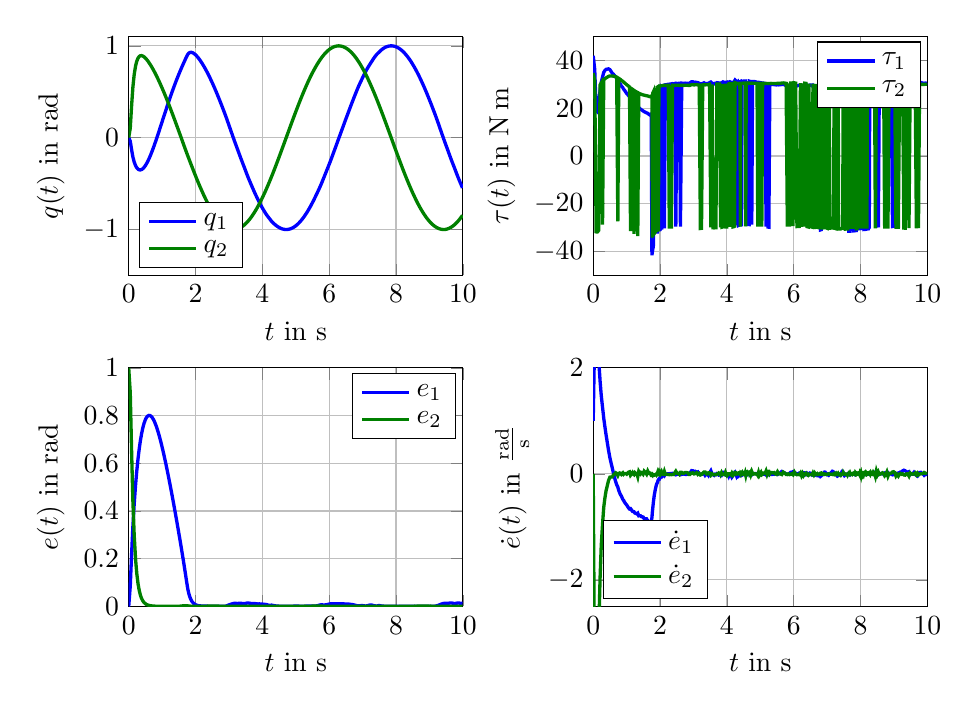
\begin{tikzpicture}

\begin{axis}[%
width=0.35\textwidth,
height=0.25\textwidth,
scale only axis,
xmin=0,
xmax=10,
xlabel={$t$ in $\mathrm{s}$},
xmajorgrids,
ymin=-1.5,
ymax=1.1,
ylabel={$q(t)$ in $\mathrm{rad}$},
ymajorgrids,
name=plot1,
legend style={at={(0.03,0.03)},anchor=south west,draw=black,fill=white,legend cell align=left}
]
\addplot [
color=blue,
solid,
line width=1.2pt
]
table[row sep=crcr]{
0 0\\
0.0463148688495906 -0.0388202463871081\\
0.0884827641908161 -0.136033823991418\\
0.125079420841395 -0.210573874209455\\
0.16420255774314 -0.265772582722689\\
0.206039685231688 -0.305992195045621\\
0.240769322133752 -0.328265625745732\\
0.279410337217424 -0.343761448331423\\
0.316163866862022 -0.35097338365754\\
0.349490418965392 -0.35199529855969\\
0.384544881158941 -0.347938834198776\\
0.419654179681859 -0.33919255992128\\
0.457624535004164 -0.324954765078235\\
0.499618483904862 -0.30400861278917\\
0.533393778421568 -0.2836945265231\\
0.567498764299021 -0.260329842508671\\
0.606481986067105 -0.230503008423891\\
0.637220720612916 -0.204982856376619\\
0.672234955532208 -0.173898887528336\\
0.703167435153003 -0.144911163101915\\
0.737346702155619 -0.111430115569781\\
0.765522837894485 -0.0829265422225078\\
0.792639464925439 -0.0547878165202565\\
0.819318909514715 -0.0264813676132645\\
0.845118464783689 0.00136433404520112\\
0.887241781336159 0.0476763746149297\\
0.910668585068524 0.0736778050352429\\
0.934230606843112 0.0999847842535443\\
0.969604870093779 0.139758144295941\\
1.00234627779788 0.176620134402025\\
1.02424226705366 0.201219714771649\\
1.05288252511947 0.233341951892669\\
1.08643835845195 0.270811461784024\\
1.1175360450147 0.305277855266618\\
1.14809220501846 0.338843006059372\\
1.17674729911475 0.370021496453866\\
1.20022361042454 0.395296868949841\\
1.22334221840217 0.41994941135235\\
1.24990820994572 0.447945136424655\\
1.27714934906042 0.476239731098085\\
1.30536994776385 0.505109354415333\\
1.33380595732101 0.533682530030559\\
1.36344095282278 0.562962554240135\\
1.39049128771628 0.589233544020903\\
1.41430218778294 0.611976261553886\\
1.43908310093511 0.635229082582662\\
1.4660300662014 0.660019192944941\\
1.49250918263224 0.683916288643247\\
1.52593566916944 0.713380242113357\\
1.56180259382082 0.74420972984838\\
1.59841737533143 0.775142063663434\\
1.63218706049736 0.802680215820098\\
1.66915388631813 0.832587496839341\\
1.70214356439556 0.859003627372797\\
1.73656845174845 0.885622632828779\\
1.75758548712615 0.900424909409077\\
1.76916543282678 0.907231062050544\\
1.78319339625967 0.914022280482348\\
1.79974311126162 0.920192378663348\\
1.82579806448608 0.926386403391646\\
1.85951331800078 0.929103657566523\\
1.87784175476544 0.92855991095091\\
1.89435712554127 0.927093716042315\\
1.91036209051348 0.924903598431597\\
1.92507942245533 0.922287816579729\\
1.93936784853061 0.919248047513937\\
1.95260530178687 0.916030020823779\\
1.9662957307571 0.912315150651362\\
1.97962651518193 0.908364576102559\\
1.99316455160314 0.904028701493279\\
2.00686332538074 0.899317491826224\\
2.02083398387401 0.89420873689901\\
2.03494902386748 0.888746383707691\\
2.04967364084416 0.882742970554658\\
2.06495539171365 0.87621354338659\\
2.08376190420839 0.867721567507402\\
2.10733167268852 0.856443789291659\\
2.13132784134452 0.844353888391433\\
2.15802559876606 0.830177819445341\\
2.18826491113502 0.813297420882452\\
2.21800887604122 0.795963930098746\\
2.24779026330602 0.777833797946683\\
2.27754977898812 0.758973672943643\\
2.30666189252561 0.739873757789382\\
2.33999550814542 0.717139611201249\\
2.37460639476268 0.692690105250372\\
2.40674618040462 0.66919878818081\\
2.43857377105191 0.645288801118553\\
2.47250045685697 0.619028039261085\\
2.50711777602187 0.591475228329423\\
2.5419364277243 0.563065101825361\\
2.57791179808931 0.533061925305377\\
2.61087372090297 0.504982387007435\\
2.64998901658833 0.470843831589601\\
2.68366687186223 0.440933968749047\\
2.71533327327976 0.412332437283429\\
2.7519096997959 0.37873820831918\\
2.78909031019028 0.344094519910912\\
2.82480197933786 0.310341405458928\\
2.86124432753857 0.275509370737825\\
2.89281156232636 0.244970117997409\\
2.91766006227628 0.220377946522039\\
2.94553617583797 0.191314236187151\\
2.98105407786228 0.154327969186816\\
3.01820294596371 0.115558461028118\\
3.05497277797894 0.0771365615974421\\
3.09328729995699 0.0372068718664149\\
3.13180117713514 -0.00267002414985816\\
3.17367139945043 -0.0456492515065139\\
3.20788114926555 -0.0795151862978449\\
3.24131037343297 -0.112079905040435\\
3.27764119743609 -0.148579621853138\\
3.31506530543054 -0.185802038055204\\
3.35106572797567 -0.221278029294494\\
3.38667825304921 -0.255408781487283\\
3.41820702754088 -0.285417433094941\\
3.44947001164456 -0.314824175226425\\
3.48266468978309 -0.346759016702483\\
3.5211315159232 -0.384203159171535\\
3.55810207383413 -0.419098542112252\\
3.58784629973275 -0.445834811103801\\
3.61743978338724 -0.471605536263606\\
3.64580507785454 -0.496023796375532\\
3.67307429901967 -0.519152631787308\\
3.70193092846579 -0.543472261798775\\
3.73196656643788 -0.569002176361142\\
3.75844830031468 -0.590620038119512\\
3.78700279510185 -0.613364972534334\\
3.81011762923894 -0.631334524684465\\
3.83681974239327 -0.651633514880157\\
3.85794134005838 -0.667236845273303\\
3.88339343882865 -0.686286257943254\\
3.91039437399401 -0.706146565905443\\
3.93302010848701 -0.721940779303543\\
3.9561888026892 -0.737868472117936\\
3.97691133204355 -0.751713424440889\\
3.99817489505322 -0.765578251202779\\
4.01799065971972 -0.778117811259992\\
4.03650134113722 -0.789637239010214\\
4.05491334196152 -0.800636189753301\\
4.06979398514194 -0.809289298978993\\
4.08869639105072 -0.820360206818781\\
4.10803648306297 -0.831298171981994\\
4.12667240417748 -0.841173880069045\\
4.14969557503799 -0.852518608171833\\
4.16562961911884 -0.860127583636351\\
4.18104341612508 -0.867411736536874\\
4.19509395874954 -0.874017334722459\\
4.20852869918637 -0.88028352971349\\
4.22144000743875 -0.886320045588726\\
4.23377529448321 -0.892165039630822\\
4.24649855038009 -0.898346661487451\\
4.26990302615732 -0.909352169197385\\
4.29603263120914 -0.91973173286964\\
4.30857694367181 -0.924300328552323\\
4.32334050312884 -0.929492944440826\\
4.33699745384296 -0.934134604592384\\
4.35131949725186 -0.938892341070675\\
4.36565442070485 -0.943516146041763\\
4.37796900607947 -0.9473478264585\\
4.38991486474948 -0.950948469650836\\
4.40310351396593 -0.954795135381597\\
4.41501912756036 -0.958188136801429\\
4.42700867086476 -0.961473762748617\\
4.4391221924609 -0.964658508088252\\
4.45362822536477 -0.968337366914414\\
4.46467307197818 -0.970975008492251\\
4.47835411235924 -0.974117087253655\\
4.49219002240913 -0.977163914395356\\
4.50627541521124 -0.980080774761068\\
4.52006531195363 -0.982759172080447\\
4.5358967085836 -0.985582800614273\\
4.54772646790811 -0.987527387684393\\
4.56452435311369 -0.990257796976715\\
4.57950427745589 -0.992283140284153\\
4.59514713033864 -0.994182014955933\\
4.61017460954574 -0.995773771486843\\
4.62494337497317 -0.997134266637777\\
4.6408385184653 -0.998414558793523\\
4.65824279200204 -0.999509332309369\\
4.67043119440795 -1.00005690740521\\
4.68227154763727 -1.00044264839222\\
4.69471319711615 -1.00070873135564\\
4.70776546846387 -1.00081981822868\\
4.71987071885731 -1.00076803181466\\
4.74519846560075 -1.00040038956828\\
4.76868597655726 -0.999467701266902\\
4.79215769971906 -0.99792106621554\\
4.81111657741889 -0.996252155715868\\
4.83502065353915 -0.993683501161651\\
4.85823752282836 -0.990610736401759\\
4.88100876307009 -0.987084619210973\\
4.90303939450965 -0.983160804126237\\
4.92480653965485 -0.978818080484369\\
4.94919052995859 -0.973448875366256\\
4.97390034791835 -0.967386457563794\\
4.99744896904853 -0.961031133685143\\
5.01936747933123 -0.954578090059325\\
5.04562275485225 -0.946308138104729\\
5.06987127382839 -0.93809311119691\\
5.09531557550952 -0.928872330463993\\
5.12010596358194 -0.919309664979723\\
5.14563694659618 -0.908888010568255\\
5.17272649864595 -0.897182641294626\\
5.20012466462249 -0.884673955451922\\
5.22837219925343 -0.871067055511024\\
5.25725889569682 -0.856455522914069\\
5.28600494391351 -0.841222279043825\\
5.31696444195878 -0.824067169270265\\
5.34687819112671 -0.806697714094447\\
5.37885549804774 -0.787324230088031\\
5.41215599577109 -0.766320970853298\\
5.44419833268925 -0.745315154941032\\
5.47969166446526 -0.721172234046971\\
5.51754411697281 -0.694438925321489\\
5.55847032675889 -0.664487445909054\\
5.60097960170432 -0.632612440141011\\
5.64385015781572 -0.599843346877216\\
5.68727608555558 -0.566200044224049\\
5.73119442002323 -0.530853609797791\\
5.77379958958322 -0.494635251789863\\
5.80977916198983 -0.462451612486143\\
5.84034530842105 -0.434964612834281\\
5.87468074773995 -0.403764786602598\\
5.90682262831214 -0.374480256803817\\
5.94281176531904 -0.341996952871642\\
5.98001202623291 -0.307964976908798\\
6.0190351040978 -0.271767862448867\\
6.05820279399155 -0.234653341428961\\
6.09706826600496 -0.19630833682526\\
6.13043609885496 -0.16305999674652\\
6.16588222942796 -0.128107950919004\\
6.20281562792637 -0.0917502641343931\\
6.23410379240896 -0.0603992120819207\\
6.26487329838129 -0.0292110408622832\\
6.29607531243174 0.00200995513972742\\
6.33107964485188 0.0364319764837094\\
6.36528412509617 0.070662133173177\\
6.39844925472413 0.10372300748848\\
6.43117614531055 0.136278186370824\\
6.45689800270783 0.162211950864748\\
6.48588042352239 0.190915336930037\\
6.51819964642262 0.222401468513555\\
6.54956394665396 0.252818500520713\\
6.57648922136011 0.279007319066291\\
6.60374614322017 0.305545012298451\\
6.62786963430868 0.328807780815787\\
6.65303423745995 0.352876028776308\\
6.67896478433076 0.377421257644819\\
6.70417888197055 0.401144865670441\\
6.72781179707865 0.42322101861714\\
6.75167398212822 0.445407469338551\\
6.77709598202702 0.468716341349024\\
6.79943630441037 0.489163261909067\\
6.82373593830336 0.510983894829168\\
6.8445342029347 0.529298365215625\\
6.86306316380769 0.545311441373046\\
6.882362447315 0.561577787223309\\
6.90200928243025 0.577751498895312\\
6.92248204335855 0.593954482014086\\
6.94250806580296 0.60919095179041\\
6.96236527944323 0.624378512226817\\
6.98034727469117 0.63816791541576\\
6.99880818586592 0.652400896231725\\
7.01597358572502 0.665683116920681\\
7.03219421897563 0.677922037993588\\
7.05150436082282 0.692333998123903\\
7.06730837010514 0.703869882675622\\
7.08276944915351 0.714835693130941\\
7.09795728871721 0.72529635961012\\
7.11294157933918 0.735317015061982\\
7.12768971665122 0.744884455293447\\
7.14222979085905 0.754031121150587\\
7.1565497264348 0.762752162436769\\
7.17513559931615 0.773745678067334\\
7.19210510654684 0.783756530747419\\
7.20814598888297 0.793094006019365\\
7.22432574510823 0.802483212007014\\
7.23898514877626 0.810895044584994\\
7.25328602866025 0.818981301509677\\
7.2679726065233 0.827175990143272\\
7.2889909317118 0.839267553878986\\
7.30337410696217 0.847535388848931\\
7.31786823656483 0.855620926393711\\
7.33154864498282 0.863009968609108\\
7.34462803900043 0.869859583133444\\
7.35897775374929 0.877133586501154\\
7.37205414205059 0.883553188554273\\
7.3863990054164 0.890368162104557\\
7.39862021347205 0.895973240582169\\
7.4115063164008 0.901728442231877\\
7.42226033735138 0.906339548364135\\
7.43283153625763 0.910574516002158\\
7.44332514766407 0.914503218849936\\
7.45465417438787 0.918476971687654\\
7.46672531011668 0.922577177038973\\
7.47990947488531 0.927034254344742\\
7.49280869917807 0.931622990556212\\
7.50558139735666 0.936219645313264\\
7.51745534714836 0.940542347899672\\
7.52845040727831 0.944422814884817\\
7.54223171288017 0.949084137105746\\
7.55460232106751 0.953083484308641\\
7.56695801110464 0.956899526659822\\
7.57966943340661 0.960641879107753\\
7.59363114915886 0.964550382696937\\
7.60779227076719 0.968293803417469\\
7.62012409014337 0.971370159414744\\
7.63383531570471 0.974611078994064\\
7.64841296036968 0.977811171778996\\
7.65979377564655 0.980165325213779\\
7.67323642608295 0.982761281362678\\
7.68655422983193 0.98514787039491\\
7.69824673400563 0.987092652854764\\
7.71043772165344 0.988963867408769\\
7.72490550211552 0.990962216524847\\
7.74146026699154 0.992962143142313\\
7.75186466324236 0.994106442333663\\
7.7623444688697 0.99515099816233\\
7.77696535410213 0.996397956864342\\
7.79281368815349 0.997498186816308\\
7.80752335341726 0.998304212946277\\
7.82001562084599 0.998829597601042\\
7.83817732967168 0.999279246487867\\
7.84902271299636 0.999409994608682\\
7.85966814772426 0.999434929505909\\
7.87015481026306 0.99934372523788\\
7.88081200948365 0.999139240397255\\
7.8937718978428 0.998711740229548\\
7.90447820621957 0.998248046483438\\
7.91524178127672 0.997660102029843\\
7.92789508524028 0.996804287949837\\
7.94076695565831 0.99576423892922\\
7.95286651763316 0.994643686572934\\
7.96453733961557 0.99342476225841\\
7.97642717310013 0.992044506813326\\
7.98789496121187 0.990579363418904\\
7.99968570225789 0.988943097694521\\
8.0104437550157 0.98733931833303\\
8.0214301711791 0.985574089452842\\
8.03233301207958 0.983699124807995\\
8.04368333110004 0.981625944686448\\
8.05660759108537 0.979096058516225\\
8.06798563729963 0.97674772358039\\
8.07962370771765 0.974224839715977\\
8.09166646327825 0.971469843874093\\
8.10395948965456 0.968509994919246\\
8.11626521405379 0.965401739678055\\
8.12861246617709 0.962135320818756\\
8.14125018984994 0.958635952788974\\
8.15385787065634 0.954993808605987\\
8.16677413176455 0.951101992252412\\
8.17997735918837 0.94695866297855\\
8.1931922596294 0.942651064461868\\
8.20660309668311 0.93810113679301\\
8.22002014949046 0.93337820676535\\
8.23366878918196 0.928408443767638\\
8.2475643193762 0.923163254238014\\
8.26132217388808 0.917796457051182\\
8.27560963107639 0.912033943266397\\
8.28951241274158 0.906248316327635\\
8.30679463842717 0.898757098870895\\
8.32977531420581 0.888366421320446\\
8.35229103235963 0.877730517993279\\
8.37654732400844 0.865772294811773\\
8.40037471979656 0.853577146362419\\
8.42032959259816 0.843043626128193\\
8.44418641495044 0.829958153990457\\
8.47398376201266 0.812929059446808\\
8.5045414625431 0.794771676184523\\
8.53326354911131 0.777037694913246\\
8.56134992306216 0.759077266727299\\
8.59290513659896 0.738133373778973\\
8.62600026789984 0.715396021754569\\
8.6606181427953 0.690796118578396\\
8.69252903823622 0.667415702664549\\
8.72264842680324 0.644681554569317\\
8.75426108550359 0.620203116892975\\
8.78747779980547 0.593832543686902\\
8.82074694233045 0.566789347249434\\
8.85311417753001 0.539908270644498\\
8.88478200117011 0.513049883799301\\
8.91906420180116 0.483333947079982\\
8.95708661757394 0.449702925192719\\
8.98959182313584 0.420375776906997\\
9.02363138926556 0.389304899116287\\
9.05984236116275 0.355702670389303\\
9.09351664059504 0.324070719375763\\
9.13120362718501 0.288120207595569\\
9.16856083562435 0.252118530384727\\
9.19340352217752 0.227592985188471\\
9.22757765725191 0.192635027713401\\
9.2599693618867 0.159648658177301\\
9.29706395950853 0.120579564978402\\
9.33624810757238 0.0793747264214276\\
9.37380650407086 0.0400967095060471\\
9.41223267333114 9.74118389313997e-05\\
9.44976307106603 -0.038465948689606\\
9.48454896511149 -0.0734718745753117\\
9.51826330639894 -0.106462825189513\\
9.55728855682 -0.145608653526361\\
9.59712745212773 -0.185557049024572\\
9.6358184192683 -0.224245089857157\\
9.67217561086846 -0.259270247567836\\
9.70374959780059 -0.288768271053425\\
9.73402020799888 -0.316768179006895\\
9.76649974456229 -0.347303197851393\\
9.80557263752835 -0.38537530234217\\
9.83786966451013 -0.415602518449652\\
9.87349131435793 -0.448087774050071\\
9.90471469383168 -0.475634103372234\\
9.93310207279925 -0.500211131575451\\
9.96046822592932 -0.523613424740368\\
9.98842126102711 -0.547417581598331\\
};
\addlegendentry{$q_1$};

\addplot [
color=green!50!black,
solid,
line width=1.2pt
]
table[row sep=crcr]{
0 0\\
0.0463148688495906 0.103281951267142\\
0.0884827641908161 0.35802755731902\\
0.125079420841395 0.550292982412534\\
0.16420255774314 0.687678005449214\\
0.206039685231688 0.78229081450953\\
0.240769322133752 0.832000350206961\\
0.279410337217424 0.866225005498826\\
0.316163866862022 0.884338516318004\\
0.349490418965392 0.891981233333177\\
0.384544881158941 0.89313751364341\\
0.419654179681859 0.889123097347064\\
0.457624535004164 0.880281906685031\\
0.499618483904862 0.866260998330167\\
0.533393778421568 0.852610175002169\\
0.567498764299021 0.836922658682423\\
0.606481986067105 0.817016170478491\\
0.637220720612916 0.800206753351388\\
0.672234955532208 0.779668602535135\\
0.703167435153003 0.760510815697821\\
0.737346702155619 0.738304421758755\\
0.765522837894485 0.719437571714611\\
0.792639464925439 0.700682597924605\\
0.819318909514715 0.681573374339659\\
0.845118464783689 0.662574844385927\\
0.887241781336159 0.630366205841867\\
0.910668585068524 0.612118298025304\\
0.934230606843112 0.593422360710269\\
0.969604870093779 0.564510462497006\\
1.00234627779788 0.537208534241295\\
1.02424226705366 0.51872719829877\\
1.05288252511947 0.494131373668547\\
1.08643835845195 0.464747296568929\\
1.1175360450147 0.43705568576042\\
1.14809220501846 0.409424999307477\\
1.17674729911475 0.383104380013024\\
1.20022361042454 0.361318801607159\\
1.22334221840217 0.339631927458159\\
1.24990820994572 0.314486915555617\\
1.27714934906042 0.288516696272486\\
1.30536994776385 0.261375930685752\\
1.33380595732101 0.233904422358491\\
1.36344095282278 0.20497922163763\\
1.39049128771628 0.178330164861977\\
1.41430218778294 0.154731349613477\\
1.43908310093511 0.130121594785346\\
1.4660300662014 0.103341199336299\\
1.49250918263224 0.0769183277669342\\
1.52593566916944 0.0435607992989439\\
1.56180259382082 0.00760267603300708\\
1.59841737533143 -0.0299454040279509\\
1.63218706049736 -0.0639697224323577\\
1.66915388631813 -0.101379246659722\\
1.70214356439556 -0.134285408737328\\
1.73656845174845 -0.168263773341447\\
1.75758548712615 -0.188651843658415\\
1.76916543282678 -0.199625810462935\\
1.78319339625967 -0.213059447493657\\
1.79974311126162 -0.2289454146623\\
1.82579806448608 -0.253800902297312\\
1.85951331800078 -0.285910620602646\\
1.87784175476544 -0.303177926463028\\
1.89435712554127 -0.318676882522883\\
1.91036209051348 -0.333663529415339\\
1.92507942245533 -0.347392029337736\\
1.93936784853061 -0.360685182584558\\
1.95260530178687 -0.372957141743299\\
1.9662957307571 -0.38559860663886\\
1.97962651518193 -0.397971202042691\\
1.99316455160314 -0.410464309907763\\
2.00686332538074 -0.423007658076602\\
2.02083398387401 -0.435708163367697\\
2.03494902386748 -0.448425896633288\\
2.04967364084416 -0.461605750706019\\
2.06495539171365 -0.475176912698423\\
2.08376190420839 -0.491676625012996\\
2.10733167268852 -0.512113648229717\\
2.13132784134452 -0.532599025697021\\
2.15802559876606 -0.554952809243328\\
2.18826491113502 -0.579852081772017\\
2.21800887604122 -0.603989248968238\\
2.24779026330602 -0.627622134728143\\
2.27754977898812 -0.650530398140792\\
2.30666189252561 -0.672451907876055\\
2.33999550814542 -0.696786328762684\\
2.37460639476268 -0.721515253705403\\
2.40674618040462 -0.743549167504546\\
2.43857377105191 -0.764520240993454\\
2.47250045685697 -0.786049988231113\\
2.50711777602187 -0.807039813795375\\
2.5419364277243 -0.827197622853484\\
2.57791179808931 -0.846963311382088\\
2.61087372090297 -0.863943193607984\\
2.64998901658833 -0.8830464778029\\
2.68366687186223 -0.898298705619358\\
2.71533327327976 -0.911792466574177\\
2.7519096997959 -0.926275269360313\\
2.78909031019028 -0.939734752503733\\
2.82480197933786 -0.951432342659133\\
2.86124432753857 -0.962142467110401\\
2.89281156232636 -0.970399579958191\\
2.91766006227628 -0.976106381682645\\
2.94553617583797 -0.981869089781573\\
2.98105407786228 -0.988099646728433\\
3.01820294596371 -0.993365157797075\\
3.05497277797894 -0.997195594231051\\
3.09328729995699 -0.999848817129395\\
3.13180117713514 -1.00106582359471\\
3.17367139945043 -1.00063822553284\\
3.20788114926555 -0.998903545294521\\
3.24131037343297 -0.995992173875094\\
3.27764119743609 -0.991780040104804\\
3.31506530543054 -0.986086760122837\\
3.35106572797567 -0.9791225877914\\
3.38667825304921 -0.971035431876434\\
3.41820702754088 -0.962905968090573\\
3.44947001164456 -0.953941565760671\\
3.48266468978309 -0.943348889156762\\
3.5211315159232 -0.929847572403237\\
3.55810207383413 -0.915573398831069\\
3.58784629973275 -0.902999527174962\\
3.61743978338724 -0.88982343888486\\
3.64580507785454 -0.876478168714934\\
3.67307429901967 -0.862925954542322\\
3.70193092846579 -0.847950672134522\\
3.73196656643788 -0.831614307955239\\
3.75844830031468 -0.81652954198196\\
3.78700279510185 -0.799708924397288\\
3.81011762923894 -0.785523185070773\\
3.83681974239327 -0.768667367409623\\
3.85794134005838 -0.754957818993793\\
3.88339343882865 -0.738045410697877\\
3.91039437399401 -0.7195381249505\\
3.93302010848701 -0.703569529941346\\
3.9561888026892 -0.686896431900726\\
3.97691133204355 -0.671648723092431\\
3.99817489505322 -0.655713196758777\\
4.01799065971972 -0.640601018423\\
4.03650134113722 -0.62630338531668\\
4.05491334196152 -0.611809401637558\\
4.06979398514194 -0.599941511843405\\
4.08869639105072 -0.584715895614197\\
4.10803648306297 -0.568907519758479\\
4.12667240417748 -0.553475230366435\\
4.14969557503799 -0.534148330802327\\
4.16562961911884 -0.520591350310165\\
4.18104341612508 -0.507314945002153\\
4.19509395874954 -0.495118777549637\\
4.20852869918637 -0.483370056638958\\
4.22144000743875 -0.472005996901458\\
4.23377529448321 -0.461082775419805\\
4.24649855038009 -0.449770612592511\\
4.26990302615732 -0.428869304382354\\
4.29603263120914 -0.40519804954344\\
4.30857694367181 -0.393694309587961\\
4.32334050312884 -0.38005713048263\\
4.33699745384296 -0.367356415397545\\
4.35131949725186 -0.353975400936297\\
4.36565442070485 -0.340552772890462\\
4.37796900607947 -0.328971668088192\\
4.38991486474948 -0.317665357700969\\
4.40310351396593 -0.305124425297847\\
4.41501912756036 -0.293764143722112\\
4.42700867086476 -0.282299236704561\\
4.4391221924609 -0.270688343692083\\
4.45362822536477 -0.256579634433193\\
4.46467307197818 -0.245869883741907\\
4.47835411235924 -0.232635041553935\\
4.49219002240913 -0.219156321340581\\
4.50627541521124 -0.205408528317862\\
4.52006531195363 -0.191887107693907\\
4.5358967085836 -0.176308508933166\\
4.54772646790811 -0.164697654026255\\
4.56452435311369 -0.147992534273711\\
4.57950427745589 -0.133225903949014\\
4.59514713033864 -0.117719535666776\\
4.61017460954574 -0.102848390919175\\
4.62494337497317 -0.0882028269867254\\
4.6408385184653 -0.0724126056578713\\
4.65824279200204 -0.0550603429760444\\
4.67043119440795 -0.0429443235618671\\
4.68227154763727 -0.031135830316462\\
4.69471319711615 -0.0187136715052607\\
4.70776546846387 -0.00567227168457047\\
4.71987071885731 0.00641941702891874\\
4.74519846560075 0.0317211091866469\\
4.76868597655726 0.0551609724109684\\
4.79215769971906 0.078529658651747\\
4.81111657741889 0.0973989557331558\\
4.83502065353915 0.121171871165753\\
4.85823752282836 0.144168550282304\\
4.88100876307009 0.166680675623996\\
4.90303939450965 0.18836281201202\\
4.92480653965485 0.209706663300442\\
4.94919052995859 0.2334161422213\\
4.97390034791835 0.257321268810112\\
4.99744896904853 0.280070268524157\\
5.01936747933123 0.300992504712267\\
5.04562275485225 0.325920864201399\\
5.06987127382839 0.348777403548387\\
5.09531557550952 0.372470134102417\\
5.12010596358194 0.395345233880817\\
5.14563694659618 0.41867196545506\\
5.17272649864595 0.443063944289956\\
5.20012466462249 0.467424272550646\\
5.22837219925343 0.49215650857239\\
5.25725889569682 0.517003456698086\\
5.28600494391351 0.541367678065606\\
5.31696444195878 0.567229361833026\\
5.34687819112671 0.591678632078368\\
5.37885549804774 0.61712725567135\\
5.41215599577109 0.642945706328692\\
5.44419833268925 0.667144707181189\\
5.47969166446526 0.692891699397388\\
5.51754411697281 0.719378156028401\\
5.55847032675889 0.746924888303695\\
5.60097960170432 0.774367703802518\\
5.64385015781572 0.800622759226017\\
5.68727608555558 0.825825272265576\\
5.73119442002323 0.84980091873502\\
5.77379958958322 0.871583511284254\\
5.80977916198983 0.888767844341891\\
5.84034530842105 0.902415477765244\\
5.87468074773995 0.916707845160865\\
5.90682262831214 0.929056830444989\\
5.94281176531904 0.941715548346106\\
5.98001202623291 0.953510193686107\\
6.0190351040978 0.96443441396798\\
6.05820279399155 0.973889938010282\\
6.09706826600496 0.981823614651155\\
6.13043609885496 0.987459374682469\\
6.16588222942796 0.992202673627937\\
6.20281562792637 0.995829549624565\\
6.23410379240896 0.997841507829087\\
6.26487329838129 0.999004452425502\\
6.29607531243174 0.999018209671944\\
6.33107964485188 0.997928480471538\\
6.36528412509617 0.995760822253478\\
6.39844925472413 0.992548758157816\\
6.43117614531055 0.98827741633909\\
6.45689800270783 0.984233320403684\\
6.48588042352239 0.978739712750435\\
6.51819964642262 0.971753375332436\\
6.54956394665396 0.963942116699579\\
6.57648922136011 0.956544099262377\\
6.60374614322017 0.948333706902311\\
6.62786963430868 0.940546636523391\\
6.65303423745995 0.931770224393614\\
6.67896478433076 0.922128019450357\\
6.70417888197055 0.912173803492143\\
6.72781179707865 0.902288155524823\\
6.75167398212822 0.891808006721484\\
6.77709598202702 0.88004315791071\\
6.79943630441037 0.869267606305256\\
6.82373593830336 0.857071792278674\\
6.8445342029347 0.846207283133903\\
6.86306316380769 0.836215292819425\\
6.882362447315 0.825482806025315\\
6.90200928243025 0.814227641601347\\
6.92248204335855 0.802165769020497\\
6.94250806580296 0.790053725186048\\
6.96236527944323 0.777720666816799\\
6.98034727469117 0.766286545939469\\
6.99880818586592 0.75427088822592\\
7.01597358572502 0.742918464009663\\
7.03219421897563 0.731985607413434\\
7.05150436082282 0.718742136679586\\
7.06730837010514 0.707668100732989\\
7.08276944915351 0.696662116176357\\
7.09795728871721 0.68568948813216\\
7.11294157933918 0.674705964828209\\
7.12768971665122 0.663748268343749\\
7.14222979085905 0.652796276417891\\
7.1565497264348 0.641880263110729\\
7.17513559931615 0.627466752722277\\
7.19210510654684 0.614167810538941\\
7.20814598888297 0.601433635875878\\
7.22432574510823 0.588414977372583\\
7.23898514877626 0.576502694521786\\
7.25328602866025 0.564747309954517\\
7.2679726065233 0.552557513318852\\
7.2889909317118 0.534862683991058\\
7.30337410696217 0.522702002604733\\
7.31786823656483 0.510336073973818\\
7.33154864498282 0.498564294518121\\
7.34462803900043 0.487212384725531\\
7.35897775374929 0.474662254897742\\
7.37205414205059 0.463082357595758\\
7.3863990054164 0.450326942322015\\
7.39862021347205 0.439382491087147\\
7.4115063164008 0.42777681932713\\
7.42226033735138 0.418023399232095\\
7.43283153625763 0.408403255974588\\
7.44332514766407 0.398794652202628\\
7.45465417438787 0.388347241236813\\
7.46672531011668 0.377162127309406\\
7.47990947488531 0.364897267792346\\
7.49280869917807 0.352833263035342\\
7.50558139735666 0.340832643608594\\
7.51745534714836 0.329679950583558\\
7.52845040727831 0.31932861890672\\
7.54223171288017 0.306267685363402\\
7.55460232106751 0.294497339663453\\
7.56695801110464 0.282680363567469\\
7.57966943340661 0.270485288927615\\
7.59363114915886 0.257016750125571\\
7.60779227076719 0.243283579176314\\
7.62012409014337 0.231321693388236\\
7.63383531570471 0.217939244559272\\
7.64841296036968 0.203687124238757\\
7.65979377564655 0.192543206506672\\
7.67323642608295 0.179331456004222\\
7.68655422983193 0.166203058121758\\
7.69824673400563 0.154671899391437\\
7.71043772165344 0.142628327078008\\
7.72490550211552 0.128307392549301\\
7.74146026699154 0.111877823028895\\
7.75186466324236 0.101496195762065\\
7.7623444688697 0.0910574872672164\\
7.77696535410213 0.0764664888320961\\
7.79281368815349 0.0606827329055656\\
7.80752335341726 0.0459783734175499\\
7.82001562084599 0.0334809720916305\\
7.83817732967168 0.0152811026281642\\
7.84902271299636 0.00440644481185814\\
7.85966814772426 -0.00626834048293753\\
7.87015481026306 -0.0167795785993047\\
7.88081200948365 -0.0274593551282727\\
7.8937718978428 -0.0403733932422961\\
7.90447820621957 -0.0511035679595083\\
7.91524178127672 -0.0618371493901931\\
7.92789508524028 -0.0743932195334825\\
7.94076695565831 -0.0871586376782168\\
7.95286651763316 -0.0991612149270566\\
7.96453733961557 -0.110712335441636\\
7.97642717310013 -0.122481751371664\\
7.98789496121187 -0.133817306340846\\
7.99968570225789 -0.145476504951126\\
8.0104437550157 -0.156117090360787\\
8.0214301711791 -0.166942685550076\\
8.03233301207958 -0.177652680427471\\
8.04368333110004 -0.188790826054537\\
8.05660759108537 -0.201435832219181\\
8.06798563729963 -0.212553228242057\\
8.07962370771765 -0.224005165493571\\
8.09166646327825 -0.235822574514101\\
8.10395948965456 -0.24783760575893\\
8.11626521405379 -0.259820435883065\\
8.12861246617709 -0.271804667883879\\
8.14125018984994 -0.28401334053988\\
8.15385787065634 -0.296150025324496\\
8.16677413176455 -0.308523929459444\\
8.17997735918837 -0.321108671720889\\
8.1931922596294 -0.333656855603819\\
8.20660309668311 -0.346320931558751\\
8.22002014949046 -0.358914861040242\\
8.23366878918196 -0.371653321757734\\
8.2475643193762 -0.384541747365206\\
8.26132217388808 -0.397223039899905\\
8.27560963107639 -0.410331180973493\\
8.28951241274158 -0.422966530792973\\
8.30679463842717 -0.438530366686502\\
8.32977531420581 -0.459112292170314\\
8.35229103235963 -0.479013550843754\\
8.37654732400844 -0.500139234363124\\
8.40037471979656 -0.520654624611339\\
8.42032959259816 -0.537594693367776\\
8.44418641495044 -0.557542625337547\\
8.47398376201266 -0.582063351331039\\
8.5045414625431 -0.606779286899608\\
8.53326354911131 -0.629508397147799\\
8.56134992306216 -0.651148307086451\\
8.59290513659896 -0.674716262232773\\
8.62600026789984 -0.698921856474582\\
8.6606181427953 -0.723560736508996\\
8.69252903823622 -0.745322936515353\\
8.72264842680324 -0.765109372012349\\
8.75426108550359 -0.785125164735112\\
8.78747779980547 -0.805322139117519\\
8.82074694233045 -0.824695424959701\\
8.85311417753001 -0.842554807506009\\
8.88478200117011 -0.859144150449711\\
8.91906420180116 -0.876227070861683\\
8.95708661757394 -0.893973927773234\\
8.98959182313584 -0.908059995649615\\
9.02363138926556 -0.921955915145838\\
9.05984236116275 -0.93542261131457\\
9.09351664059504 -0.946831920890905\\
9.13120362718501 -0.958360037487398\\
9.16856083562435 -0.968440583994904\\
9.19340352217752 -0.974351347177467\\
9.22757765725191 -0.981601231883884\\
9.2599693618867 -0.987351147869319\\
9.29706395950853 -0.992755167152339\\
9.33624810757238 -0.99702339721864\\
9.37380650407086 -0.999661280826532\\
9.41223267333114 -1.00094477635676\\
9.44976307106603 -1.0007885078978\\
9.48454896511149 -0.999240167954043\\
9.51826330639894 -0.996570676715871\\
9.55728855682 -0.992225779152637\\
9.59712745212773 -0.986253625992453\\
9.6358184192683 -0.978876020249278\\
9.67217561086846 -0.970462019650793\\
9.70374959780059 -0.962222553080075\\
9.73402020799888 -0.953488533223891\\
9.76649974456229 -0.943141523070662\\
9.80557263752835 -0.929451398503806\\
9.83786966451013 -0.91693619585565\\
9.87349131435793 -0.902011921197424\\
9.90471469383168 -0.887985671845804\\
9.93310207279925 -0.874521755502843\\
9.96046822592932 -0.860798154107237\\
9.98842126102711 -0.846165960596502\\
};
\addlegendentry{$q_2$};

\end{axis}

\begin{axis}[%
width=0.35\textwidth,
height=0.25\textwidth,
scale only axis,
xmin=0,
xmax=10,
xlabel={$t$ in $\mathrm{s}$},
xmajorgrids,
ymin=0,
ymax=1,
ylabel={$e(t)$ in $\mathrm{rad}$},
ymajorgrids,
name=plot3,
at=(plot1.below south west),
anchor=above north west,
legend style={draw=black,fill=white,legend cell align=left}
]
\addplot [
color=blue,
solid,
line width=1.2pt
]
table[row sep=crcr]{
0 0\\
0.0463148688495906 0.0851185589291307\\
0.0884827641908161 0.224401175168014\\
0.125079420841395 0.335327408374958\\
0.16420255774314 0.429238249891855\\
0.206039685231688 0.51057715999106\\
0.240769322133752 0.566715453559638\\
0.279410337217424 0.619550350259682\\
0.316163866862022 0.661896245196746\\
0.349490418965392 0.694414374996342\\
0.384544881158941 0.72307612863689\\
0.419654179681859 0.746637223896933\\
0.457624535004164 0.766773080141151\\
0.499618483904862 0.783099304638042\\
0.533393778421568 0.792153126828878\\
0.567498764299021 0.797854412645834\\
0.606481986067105 0.800483396304418\\
0.637220720612916 0.799946745917656\\
0.672234955532208 0.796635128754933\\
0.703167435153003 0.791548202718163\\
0.737346702155619 0.783756278973404\\
0.765522837894485 0.775840612145837\\
0.792639464925439 0.766996387370041\\
0.819318909514715 0.757162373419431\\
0.845118464783689 0.746685401663945\\
0.887241781336159 0.727656363224437\\
0.910668585068524 0.71623609941167\\
0.934230606843112 0.704157175922246\\
0.969604870093779 0.684904137903857\\
1.00234627779788 0.666116232391128\\
1.02424226705366 0.653100891040116\\
1.05288252511947 0.635511929073346\\
1.08643835845195 0.614162625495932\\
1.1175360450147 0.593746353773704\\
1.14809220501846 0.573139963299553\\
1.17674729911475 0.553340592434925\\
1.20022361042454 0.536823220686292\\
1.22334221840217 0.520293236901565\\
1.24990820994572 0.501010535476418\\
1.27714934906042 0.480954912799601\\
1.30536994776385 0.459871386122942\\
1.33380595732101 0.438366441696009\\
1.36344095282278 0.415616238123268\\
1.39049128771628 0.394555491979186\\
1.41430218778294 0.375803501133507\\
1.43908310093511 0.356109263487781\\
1.4660300662014 0.334497840202165\\
1.49250918263224 0.313020837696989\\
1.52593566916944 0.28561368732695\\
1.56180259382082 0.255749826807829\\
1.59841737533143 0.224476499426924\\
1.63218706049736 0.195435964847488\\
1.66915388631813 0.162579296742749\\
1.70214356439556 0.132382718536905\\
1.73656845174845 0.100668605166808\\
1.75758548712615 0.0821806583202926\\
1.76916543282678 0.073158220862638\\
1.78319339625967 0.0635061320066643\\
1.79974311126162 0.0537135857406773\\
1.82579806448608 0.041276453970846\\
1.85951331800078 0.0295063083769727\\
1.87784175476544 0.0246708186450818\\
1.89435712554127 0.021015578384333\\
1.91036209051348 0.0179957904035397\\
1.92507942245533 0.0156076203069485\\
1.93936784853061 0.0135949064708223\\
1.95260530178687 0.0119621097892441\\
1.9662957307571 0.0104891238859022\\
1.97962651518193 0.00922191690746099\\
1.99316455160314 0.00809201077760657\\
2.00686332538074 0.00710239002674817\\
2.02083398387401 0.00622198528370133\\
2.03494902386748 0.00545481095877687\\
2.04967364084416 0.00476982611377219\\
2.06495539171365 0.00415432603827393\\
2.08376190420839 0.00357137710508726\\
2.10733167268852 0.00304104399451532\\
2.13132784134452 0.00261876976447228\\
2.15802559876606 0.00230119322653988\\
2.18826491113502 0.00204926802179728\\
2.21800887604122 0.00180370083208858\\
2.24779026330602 0.00162559647575722\\
2.27754977898812 0.00150041223792874\\
2.30666189252561 0.00137628053276539\\
2.33999550814542 0.00132830622994229\\
2.37460639476268 0.00127837833966848\\
2.40674618040462 0.0012744686418017\\
2.43857377105191 0.00123491574977574\\
2.47250045685697 0.00124613612467384\\
2.50711777602187 0.00127944305316852\\
2.5419364277243 0.00129360917366417\\
2.57791179808931 0.00123929077256535\\
2.61087372090297 0.00117112370334982\\
2.64998901658833 0.00119639245198683\\
2.68366687186223 0.00115457606907471\\
2.71533327327976 0.00113536142033877\\
2.7519096997959 0.00115694879253075\\
2.78909031019028 0.00115284463414839\\
2.82480197933786 0.0011771347380074\\
2.86124432753857 0.00118102170009837\\
2.89281156232636 0.0012526419450008\\
2.91766006227628 0.00168778501050509\\
2.94553617583797 0.00348864548303179\\
2.98105407786228 0.00552191094786578\\
3.01820294596371 0.00751838306730637\\
3.05497277797894 0.0093750364461275\\
3.09328729995699 0.0110796979481288\\
3.13180117713514 0.0124613441488775\\
3.17367139945043 0.0135760071133174\\
3.20788114926555 0.0132752270511693\\
3.24131037343297 0.01252736229916\\
3.27764119743609 0.0129503815303177\\
3.31506530543054 0.0131981232224438\\
3.35106572797567 0.0133335079044237\\
3.38667825304921 0.0127694143568711\\
3.41820702754088 0.0123171364979653\\
3.44947001164456 0.0117876876834683\\
3.48266468978309 0.0122614492643509\\
3.5211315159232 0.0137109714242107\\
3.55810207383413 0.0145277764547546\\
3.58784629973275 0.0142457149799486\\
3.61743978338724 0.0135139069112485\\
3.64580507785454 0.0129057722074443\\
3.67307429901967 0.0123414717890913\\
3.70193092846579 0.0119994891575351\\
3.73196656643788 0.0123304929523261\\
3.75844830031468 0.0121468670885807\\
3.78700279510185 0.0118388406083955\\
3.81011762923894 0.0115053688110683\\
3.83681974239327 0.0110736754664839\\
3.85794134005838 0.0106016411172103\\
3.88339343882865 0.0106696170533115\\
3.91039437399401 0.0108720845603887\\
3.93302010848701 0.0105835235019777\\
3.9561888026892 0.0104199214236433\\
3.97691133204355 0.0102030604924378\\
3.99817489505322 0.00996998389568404\\
4.01799065971972 0.00967894183038687\\
4.03650134113722 0.00948527874971394\\
4.05491334196152 0.00909874834894897\\
4.06979398514194 0.00874595933975131\\
4.08869639105072 0.0086328182148997\\
4.10803648306297 0.00842797182866128\\
4.12667240417748 0.00785770113499606\\
4.14969557503799 0.00669726834976425\\
4.16562961911884 0.00591370055290574\\
4.18104341612508 0.0052856744874239\\
4.19509395874954 0.00485728153566078\\
4.20852869918637 0.00455821937833001\\
4.22144000743875 0.00443419543935009\\
4.23377529448321 0.00453079841803683\\
4.24649855038009 0.00492473928528092\\
4.26990302615732 0.00566216656749352\\
4.29603263120914 0.005163120298879\\
4.30857694367181 0.0047305002195539\\
4.32334050312884 0.0042225454182826\\
4.33699745384296 0.0037704594132163\\
4.35131949725186 0.00337280390815464\\
4.36565442070485 0.0030287311665218\\
4.37796900607947 0.0027469811342572\\
4.38991486474948 0.00249423007163152\\
4.40310351396593 0.00224383398531103\\
4.41501912756036 0.00207769128642898\\
4.42700867086476 0.00191910634445458\\
4.4391221924609 0.00176410783914627\\
4.45362822536477 0.00162954513407287\\
4.46467307197818 0.00150002141243322\\
4.47835411235924 0.00137847468419405\\
4.49219002240913 0.00130990290357724\\
4.50627541521124 0.00124708252559935\\
4.52006531195363 0.00119643315325246\\
4.5358967085836 0.00111717470829731\\
4.54772646790811 0.00105365540214908\\
4.56452435311369 0.00116986747700243\\
4.57950427745589 0.00109932768534216\\
4.59514713033864 0.00104697164111589\\
4.61017460954574 0.000993113704453319\\
4.62494337497317 0.000955197855782575\\
4.6408385184653 0.000973201240352495\\
4.65824279200204 0.00097487905637661\\
4.67043119440795 0.000937006181292332\\
4.68227154763727 0.000896143989341347\\
4.69471319711615 0.000864943945483643\\
4.70776546846387 0.000830506640882578\\
4.71987071885731 0.000796019889393484\\
4.74519846560075 0.000938572447955921\\
4.76868597655726 0.00105195866719732\\
4.79215769971906 0.00110090384930461\\
4.81111657741889 0.0011217675970846\\
4.83502065353915 0.00119334629350165\\
4.85823752282836 0.0012277947081657\\
4.88100876307009 0.00126728273730503\\
4.90303939450965 0.00127961320603076\\
4.92480653965485 0.00129398752748189\\
4.94919052995859 0.0013555901745822\\
4.97390034791835 0.0013861262101853\\
4.99744896904853 0.00138634901430124\\
5.01936747933123 0.00132713373113225\\
5.04562275485225 0.00131862134033622\\
5.06987127382839 0.00131233156074895\\
5.09531557550952 0.00129720435981162\\
5.12010596358194 0.0012812012519563\\
5.14563694659618 0.00128103525856249\\
5.17272649864595 0.00128003539792199\\
5.20012466462249 0.00127771405057797\\
5.22837219925343 0.00125902335638839\\
5.25725889569682 0.00126080111348026\\
5.28600494391351 0.00127809343906693\\
5.31696444195878 0.00132368440952535\\
5.34687819112671 0.00132313395563444\\
5.37885549804774 0.00131321895313441\\
5.41215599577109 0.00132871151974712\\
5.44419833268925 0.00134857380790443\\
5.47969166446526 0.00138648163435307\\
5.51754411697281 0.00143952584644325\\
5.55847032675889 0.00156536716846378\\
5.60097960170432 0.00210585069144165\\
5.64385015781572 0.00318131133846655\\
5.68727608555558 0.00493855098779883\\
5.73119442002323 0.00647013773640126\\
5.77379958958322 0.00699420857225208\\
5.80977916198983 0.00653114909417474\\
5.84034530842105 0.00645737534805352\\
5.87468074773995 0.00652740349757586\\
5.90682262831214 0.00694008510233424\\
5.94281176531904 0.00815772567352635\\
5.98001202623291 0.00941471215708778\\
6.0190351040978 0.0106788214031847\\
6.05820279399155 0.011564025372583\\
6.09706826600496 0.0112639380240488\\
6.13043609885496 0.0109040947558556\\
6.16588222942796 0.0110737034392084\\
6.20281562792637 0.0114670787239079\\
6.23410379240896 0.0113374011258535\\
6.26487329838129 0.0109000554734634\\
6.29607531243174 0.0108796931648569\\
6.33107964485188 0.0114440527438191\\
6.36528412509617 0.0113444885269805\\
6.39844925472413 0.0112858810191225\\
6.43117614531055 0.0111730446716393\\
6.45689800270783 0.0106283999401012\\
6.48588042352239 0.0103946625862975\\
6.51819964642262 0.0104554620944123\\
6.54956394665396 0.0104210329270035\\
6.57648922136011 0.010109295103183\\
6.60374614322017 0.00955386425179366\\
6.62786963430868 0.00909180759653166\\
6.65303423745995 0.00859855263207232\\
6.67896478433076 0.00810626892134314\\
6.70417888197055 0.00752260812418526\\
6.72781179707865 0.00689969746432234\\
6.75167398212822 0.00613084984505735\\
6.77709598202702 0.00535645621920133\\
6.79943630441037 0.00445993522162413\\
6.82373593830336 0.00362429995353497\\
6.8445342029347 0.00303020792960462\\
6.86306316380769 0.00261032296257313\\
6.882362447315 0.00238535953680918\\
6.90200928243025 0.00232611885892786\\
6.92248204335855 0.00267672678681963\\
6.94250806580296 0.00339074419271579\\
6.96236527944323 0.00377666925219688\\
6.98034727469117 0.00387653335891569\\
6.99880818586592 0.00368672473862763\\
7.01597358572502 0.00326167690304524\\
7.03219421897563 0.00299121916976186\\
7.05150436082282 0.00259348825428996\\
7.06730837010514 0.00233469172914225\\
7.08276944915351 0.00223060467100322\\
7.09795728871721 0.0022728294162111\\
7.11294157933918 0.00244984812029725\\
7.12768971665122 0.00275762610345964\\
7.14222979085905 0.00318768123115509\\
7.1565497264348 0.0037419115110735\\
7.17513559931615 0.00455212815749462\\
7.19210510654684 0.00508377991489273\\
7.20814598888297 0.00550309345113331\\
7.22432574510823 0.00574697973146499\\
7.23898514877626 0.00588043020562234\\
7.25328602866025 0.00596134545031612\\
7.2679726065233 0.00597848708674142\\
7.2889909317118 0.00532602466347243\\
7.30337410696217 0.00467142929080711\\
7.31786823656483 0.00407951408811458\\
7.33154864498282 0.00359773985712797\\
7.34462803900043 0.00320030238272828\\
7.35897775374929 0.00283328009864425\\
7.37205414205059 0.00255001145227596\\
7.3863990054164 0.00229231437650457\\
7.39862021347205 0.00212889824202012\\
7.4115063164008 0.00196611482710551\\
7.42226033735138 0.00190729679086166\\
7.43283153625763 0.00204485616484107\\
7.44332514766407 0.00235572479070778\\
7.45465417438787 0.00284571356558239\\
7.46672531011668 0.00337151414977377\\
7.47990947488531 0.00381280962406438\\
7.49280869917807 0.00385999471823972\\
7.50558139735666 0.00370042061512121\\
7.51745534714836 0.00336506584898288\\
7.52845040727831 0.00305815247223773\\
7.54223171288017 0.00271414638059475\\
7.55460232106751 0.00243624636032724\\
7.56695801110464 0.00219120480710289\\
7.57966943340661 0.00196986068849214\\
7.59363114915886 0.00174943325410981\\
7.60779227076719 0.00155434788408615\\
7.62012409014337 0.00140956009945781\\
7.63383531570471 0.00125442890928018\\
7.64841296036968 0.00113389116700513\\
7.65979377564655 0.00103938665939751\\
7.67323642608295 0.000948724005548129\\
7.68655422983193 0.000868872423808065\\
7.69824673400563 0.000805157197910744\\
7.71043772165344 0.000751383065148437\\
7.72490550211552 0.000719018862218479\\
7.74146026699154 0.000714004291848536\\
7.75186466324236 0.000684149093963859\\
7.7623444688697 0.000653254160454142\\
7.77696535410213 0.000637755112308347\\
7.79281368815349 0.000631637602717672\\
7.80752335341726 0.000616795230632183\\
7.82001562084599 0.000593612831266466\\
7.83817732967168 0.000595868094365959\\
7.84902271299636 0.00057770996788109\\
7.85966814772426 0.000548902318346367\\
7.87015481026306 0.000525491797285782\\
7.88081200948365 0.000500846669388988\\
7.8937718978428 0.000496731662600336\\
7.90447820621957 0.000477272506344439\\
7.91524178127672 0.000464081887602052\\
7.92789508524028 0.000465356290348384\\
7.94076695565831 0.000472278046966923\\
7.95286651763316 0.000471185920291606\\
7.96453733961557 0.000470177809210992\\
7.97642717310013 0.000468399620844884\\
7.98789496121187 0.000467638325270192\\
7.99968570225789 0.000460830394288236\\
8.0104437550157 0.000445434045797555\\
8.0214301711791 0.000439131399502912\\
8.03233301207958 0.000438382900287526\\
8.04368333110004 0.000434583889594053\\
8.05660759108537 0.000445443686200808\\
8.06798563729963 0.000440679335684702\\
8.07962370771765 0.000425815692085774\\
8.09166646327825 0.000415849449369565\\
8.10395948965456 0.000407905146259546\\
8.11626521405379 0.000398655205444687\\
8.12861246617709 0.000390057609816474\\
8.14125018984994 0.000385409653159363\\
8.15385787065634 0.000379247764263013\\
8.16677413176455 0.000375990005270666\\
8.17997735918837 0.000373649896730277\\
8.1931922596294 0.000366553473302389\\
8.20660309668311 0.000369455554659948\\
8.22002014949046 0.000374353352270984\\
8.23366878918196 0.000372186899206928\\
8.2475643193762 0.000377777157371195\\
8.26132217388808 0.000381206842522075\\
8.27560963107639 0.000389954489708133\\
8.28951241274158 0.000397922544448925\\
8.30679463842717 0.00046288249729709\\
8.32977531420581 0.000563039760965167\\
8.35229103235963 0.000661306976862397\\
8.37654732400844 0.000769189523354696\\
8.40037471979656 0.000827113992369455\\
8.42032959259816 0.000822488841834779\\
8.44418641495044 0.000868575534392568\\
8.47398376201266 0.00094816074887738\\
8.5045414625431 0.000973196993438563\\
8.53326354911131 0.000986350075420361\\
8.56134992306216 0.000997419162645397\\
8.59290513659896 0.00106062609178814\\
8.62600026789984 0.00110794390094182\\
8.6606181427953 0.00113454313283656\\
8.69252903823622 0.0011280840343334\\
8.72264842680324 0.00116342811823755\\
8.75426108550359 0.00118792520610944\\
8.78747779980547 0.00119519435194981\\
8.82074694233045 0.00117547275511698\\
8.85311417753001 0.00112377127719332\\
8.88478200117011 0.00108264236283662\\
8.91906420180116 0.00109803358251742\\
8.95708661757394 0.00112382990159826\\
8.98959182313584 0.00120341980192956\\
9.02363138926556 0.00116924928022982\\
9.05984236116275 0.00118646540976741\\
9.09351664059504 0.00116531323175811\\
9.13120362718501 0.00125526684153204\\
9.16856083562435 0.00130445845062216\\
9.19340352217752 0.00172256726024606\\
9.22757765725191 0.00328963910116004\\
9.2599693618867 0.00441486823033624\\
9.29706395950853 0.00678753165642026\\
9.33624810757238 0.00903952944898194\\
9.37380650407086 0.0108526786592611\\
9.41223267333114 0.0124475465301516\\
9.44976307106603 0.0134834378282236\\
9.48454896511149 0.0137364532554394\\
9.51826330639894 0.0131135894194562\\
9.55728855682 0.0134855106953063\\
9.59712745212773 0.0140595461475557\\
9.6358184192683 0.0147677024517594\\
9.67217561086846 0.0143885723491539\\
9.70374959780059 0.0134010822660691\\
9.73402020799888 0.0124312634761025\\
9.76649974456229 0.0121933811264901\\
9.80557263752835 0.0137169619242892\\
9.83786966451013 0.0141596341822298\\
9.87349131435793 0.0142811566858813\\
9.90471469383168 0.0139110462074121\\
9.93310207279925 0.0134971915765159\\
9.96046822592932 0.0131786933568011\\
9.98842126102711 0.0131481111244049\\
};
\addlegendentry{$e_1$};

\addplot [
color=green!50!black,
solid,
line width=1.2pt
]
table[row sep=crcr]{
0 1\\
0.0463148688495906 0.895645706902238\\
0.0884827641908161 0.638060396250359\\
0.125079420841395 0.441894779915352\\
0.16420255774314 0.298871017994091\\
0.206039685231688 0.196557995122618\\
0.240769322133752 0.139154467324991\\
0.279410337217424 0.0949932223626753\\
0.316163866862022 0.0660966335855929\\
0.349490418965392 0.0475660917613444\\
0.384544881158941 0.0338317470775978\\
0.419654179681859 0.0241068002131107\\
0.457624535004164 0.0168226449002157\\
0.499618483904862 0.0115044082471077\\
0.533393778421568 0.00847626187573691\\
0.567498764299021 0.0063254284774934\\
0.606481986067105 0.00464212676651576\\
0.637220720612916 0.0035456775265541\\
0.672234955532208 0.00276323082989971\\
0.703167435153003 0.00228702055785102\\
0.737346702155619 0.00195062213014996\\
0.765522837894485 0.00158260255396547\\
0.792639464925439 0.00128531559289202\\
0.819318909514715 0.00114565114160681\\
0.845118464783689 0.00106782520779092\\
0.887241781336159 0.00118675760182663\\
0.910668585068524 0.00109946391692284\\
0.934230606843112 0.00101494286735637\\
0.969604870093779 0.00111496153998081\\
1.00234627779788 0.00111796156239041\\
1.02424226705366 0.00101918455099814\\
1.05288252511947 0.000937241303452796\\
1.08643835845195 0.00089297750861167\\
1.1175360450147 0.000843242714433035\\
1.14809220501846 0.000803063602995036\\
1.17674729911475 0.000825890743176128\\
1.20022361042454 0.000830530156310183\\
1.22334221840217 0.000873230218587651\\
1.24990820994572 0.000922552860889936\\
1.27714934906042 0.000928313519672597\\
1.30536994776385 0.000944808849272172\\
1.33380595732101 0.000873763521975018\\
1.36344095282278 0.000893426221633242\\
1.39049128771628 0.000999511003498404\\
1.41430218778294 0.00112480337779097\\
1.43908310093511 0.00121112623390493\\
1.4660300662014 0.00123351453028996\\
1.49250918263224 0.00128887218596126\\
1.52593566916944 0.0012848129882501\\
1.56180259382082 0.00139093569519955\\
1.59841737533143 0.00232786747652576\\
1.63218706049736 0.00261754325710553\\
1.66915388631813 0.00318019904955612\\
1.70214356439556 0.00331551470130029\\
1.73656845174845 0.00324985316156523\\
1.75758548712615 0.00294697493590912\\
1.76916543282678 0.00255512784125173\\
1.78319339625967 0.00225574075036639\\
1.79974311126162 0.0019934979524702\\
1.82579806448608 0.0015538121633375\\
1.85951331800078 0.00118806583430697\\
1.87784175476544 0.000934355557220823\\
1.89435712554127 0.000732287000637988\\
1.91036209051348 0.000585846983260363\\
1.92507942245533 0.000473956203533243\\
1.93936784853061 0.000401928462211265\\
1.95260530178687 0.000357349043005939\\
1.9662957307571 0.000329517694842685\\
1.97962651518193 0.000435005142870926\\
1.99316455160314 0.000542602448334761\\
2.00686332538074 0.000629867725779609\\
2.02083398387401 0.000708721357110531\\
2.03494902386748 0.000760593692505418\\
2.04967364084416 0.000822682712214695\\
2.06495539171365 0.000885425863243083\\
2.08376190420839 0.000913337196457309\\
2.10733167268852 0.000952400333285808\\
2.13132784134452 0.00096257441069314\\
2.15802559876606 0.000896229586655473\\
2.18826491113502 0.000879045359372777\\
2.21800887604122 0.00102423585470468\\
2.24779026330602 0.00116938116519294\\
2.27754977898812 0.00116211606408689\\
2.30666189252561 0.00122290024347815\\
2.33999550814542 0.0012262295461698\\
2.37460639476268 0.00150987609788822\\
2.40674618040462 0.00161546973521021\\
2.43857377105191 0.00162635353153329\\
2.47250045685697 0.00166491229613819\\
2.50711777602187 0.00165673751793349\\
2.5419364277243 0.00166794723938546\\
2.57791179808931 0.0016691551869612\\
2.61087372090297 0.00149979048222137\\
2.64998901658833 0.00146946648354407\\
2.68366687186223 0.00132729105778173\\
2.71533327327976 0.00127372462810293\\
2.7519096997959 0.00124571869554169\\
2.78909031019028 0.00122302787015616\\
2.82480197933786 0.00119226819712048\\
2.86124432753857 0.00118334897240824\\
2.89281156232636 0.00118631524998281\\
2.91766006227628 0.00107468431126445\\
2.94553617583797 0.00102667772294185\\
2.98105407786228 0.000958311447143201\\
3.01820294596371 0.000968014286721219\\
3.05497277797894 0.000944750615876289\\
3.09328729995699 0.00101529387562249\\
3.13180117713514 0.00111375971730832\\
3.17367139945043 0.0011527043800319\\
3.20788114926555 0.00109982321337021\\
3.24131037343297 0.00095986724693875\\
3.27764119743609 0.00102037743708405\\
3.31506530543054 0.00109544615889856\\
3.35106572797567 0.000981965987022826\\
3.38667825304921 0.000918873148281874\\
3.41820702754088 0.000920402711006352\\
3.44947001164456 0.000962611524205736\\
3.48266468978309 0.000952275528522839\\
3.5211315159232 0.00101199017234421\\
3.55810207383413 0.00106670362577688\\
3.58784629973275 0.000929212783120192\\
3.61743978338724 0.000918461332533149\\
3.64580507785454 0.000922930752232931\\
3.67307429901967 0.000868851966592366\\
3.70193092846579 0.000875296538563886\\
3.73196656643788 0.000881717472118737\\
3.75844830031468 0.000828131907526175\\
3.78700279510185 0.000855801094750586\\
3.81011762923894 0.000786402748654713\\
3.83681974239327 0.000759109783538547\\
3.85794134005838 0.000749486592932058\\
3.88339343882865 0.00079229639276257\\
3.91039437399401 0.000793806301394917\\
3.93302010848701 0.000738928289378271\\
3.9561888026892 0.000734201744640339\\
3.97691133204355 0.000707309735768491\\
3.99817489505322 0.000689421329846285\\
4.01799065971972 0.000677816820065735\\
4.03650134113722 0.000713328728741858\\
4.05491334196152 0.000688727093608454\\
4.06979398514194 0.000666648897152733\\
4.08869639105072 0.000679384263815086\\
4.10803648306297 0.000678135002979086\\
4.12667240417748 0.000678571614994405\\
4.14969557503799 0.000682060920527805\\
4.16562961911884 0.000669585092068714\\
4.18104341612508 0.000621099435514583\\
4.19509395874954 0.000587886760878897\\
4.20852869918637 0.000560383125277397\\
4.22144000743875 0.000543010754811502\\
4.23377529448321 0.000533696790172844\\
4.24649855038009 0.000552103480765953\\
4.26990302615732 0.000681986556632375\\
4.29603263120914 0.000767273142342539\\
4.30857694367181 0.000767686896088637\\
4.32334050312884 0.000748959343827627\\
4.33699745384296 0.000719595963057373\\
4.35131949725186 0.000700443449606958\\
4.36565442070485 0.000724253691019638\\
4.37796900607947 0.000750335733445018\\
4.38991486474948 0.000751244060959499\\
4.40310351396593 0.00074634098782006\\
4.41501912756036 0.000757631888145482\\
4.42700867086476 0.000776837288298693\\
4.4391221924609 0.000809900742454628\\
4.45362822536477 0.000696873566602363\\
4.46467307197818 0.000679652642486012\\
4.47835411235924 0.000730769026583172\\
4.49219002240913 0.000732539999345888\\
4.50627541521124 0.000751246637781644\\
4.52006531195363 0.000746872395984893\\
4.5358967085836 0.000731086097668698\\
4.54772646790811 0.000778236271249427\\
4.56452435311369 0.000666135695684966\\
4.57950427745589 0.000731943173114646\\
4.59514713033864 0.000746095347717482\\
4.61017460954574 0.00081191262814756\\
4.62494337497317 0.000868624519206704\\
4.6408385184653 0.000923178170386285\\
4.65824279200204 0.000940608435417274\\
4.67043119440795 0.000998847306187149\\
4.68227154763727 0.00102295041441044\\
4.69471319711615 0.00103880863959873\\
4.70776546846387 0.00104877623642732\\
4.71987071885731 0.00106225164375347\\
4.74519846560075 0.00108248998379889\\
4.76868597655726 0.0011062909761915\\
4.79215769971906 0.00115449222000251\\
4.81111657741889 0.00116833418880549\\
4.83502065353915 0.00115266639641352\\
4.85823752282836 0.00116346506783141\\
4.88100876307009 0.00114119156846099\\
4.90303939450965 0.00113475239744115\\
4.92480653965485 0.00111707276552903\\
4.94919052995859 0.00117849728535918\\
4.97390034791835 0.0012195593480695\\
4.99744896904853 0.00114475108548956\\
5.01936747933123 0.00118726671425784\\
5.04562275485225 0.00117975213155691\\
5.06987127382839 0.00113940214157471\\
5.09531557550952 0.00116656836779355\\
5.12010596358194 0.00116925486535241\\
5.14563694659618 0.00114892298332081\\
5.17272649864595 0.00118657146381806\\
5.20012466462249 0.00120253064991588\\
5.22837219925343 0.00123379048027755\\
5.25725889569682 0.00130339045368832\\
5.28600494391351 0.00130511936278832\\
5.31696444195878 0.00118347943571684\\
5.34687819112671 0.00108758293918088\\
5.37885549804774 0.00108524046141012\\
5.41215599577109 0.00109376696448238\\
5.44419833268925 0.00107211852517219\\
5.47969166446526 0.0013045773311755\\
5.51754411697281 0.00156000520821042\\
5.55847032675889 0.00176350984219154\\
5.60097960170432 0.00181619235912733\\
5.64385015781572 0.00186986712437898\\
5.68727608555558 0.00181325765567752\\
5.73119442002323 0.00168130317500992\\
5.77379958958322 0.00146071037329798\\
5.80977916198983 0.00125267848915789\\
5.84034530842105 0.00112287085197016\\
5.87468074773995 0.00100804849243397\\
5.90682262831214 0.000950815859946164\\
5.94281176531904 0.000914480023330499\\
5.98001202623291 0.000883718394583011\\
6.0190351040978 0.000880308102415905\\
6.05820279399155 0.000908070328624055\\
6.09706826600496 0.000906546925408147\\
6.13043609885496 0.000897130577352301\\
6.16588222942796 0.000925205809972018\\
6.20281562792637 0.000942545761509761\\
6.23410379240896 0.000954236407797127\\
6.26487329838129 0.000827887426580243\\
6.29607531243174 0.000898715360622582\\
6.33107964485188 0.000924804964017922\\
6.36528412509617 0.00087096230756456\\
6.39844925472413 0.000815704446039178\\
6.43117614531055 0.000791911091531872\\
6.45689800270783 0.000716532702380368\\
6.48588042352239 0.000787869349596626\\
6.51819964642262 0.000757627108068704\\
6.54956394665396 0.000788388690516117\\
6.57648922136011 0.000749786339729552\\
6.60374614322017 0.000725141640166571\\
6.62786963430868 0.000635528708603839\\
6.65303423745995 0.000611739715321358\\
6.67896478433076 0.000568315353123627\\
6.70417888197055 0.0005095456834181\\
6.72781179707865 0.000483227272377929\\
6.75167398212822 0.000443721384907003\\
6.77709598202702 0.000442493650879228\\
6.79943630441037 0.000408275419927384\\
6.82373593830336 0.000353659794266714\\
6.8445342029347 0.000330542490660557\\
6.86306316380769 0.000314288347518787\\
6.882362447315 0.000317151044450514\\
6.90200928243025 0.000333563821894978\\
6.92248204335855 0.000349776426923465\\
6.94250806580296 0.000353553213156999\\
6.96236527944323 0.000367418158846444\\
6.98034727469117 0.000380869435426812\\
6.99880818586592 0.000413836417068603\\
7.01597358572502 0.000393625772369899\\
7.03219421897563 0.000378466131410127\\
7.05150436082282 0.000337684116469728\\
7.06730837010514 0.000339737563866738\\
7.08276944915351 0.000342851206669215\\
7.09795728871721 0.000344822365184405\\
7.11294157933918 0.000349629615818969\\
7.12768971665122 0.000353620017141676\\
7.14222979085905 0.000365024731801888\\
7.1565497264348 0.00037111649295829\\
7.17513559931615 0.000428560865600836\\
7.19210510654684 0.00043040315370213\\
7.20814598888297 0.000432356449081572\\
7.22432574510823 0.000451694432148764\\
7.23898514877626 0.000452956963285511\\
7.25328602866025 0.00046913462812237\\
7.2679726065233 0.000482826142549908\\
7.2889909317118 0.000545279234037355\\
7.30337410696217 0.00050306151080437\\
7.31786823656483 0.000462470107266633\\
7.33154864498282 0.000425765129263234\\
7.34462803900043 0.000400613770702329\\
7.35897775374929 0.000372810846390681\\
7.37205414205059 0.000405634630745\\
7.3863990054164 0.000402770176067657\\
7.39862021347205 0.000404443961424916\\
7.4115063164008 0.00040088623677359\\
7.42226033735138 0.000411384534737602\\
7.43283153625763 0.000407068681618383\\
7.44332514766407 0.000416667108539936\\
7.45465417438787 0.000451562307854869\\
7.46672531011668 0.000487209093886054\\
7.47990947488531 0.000511740718189158\\
7.49280869917807 0.000538473613189261\\
7.50558139735666 0.000561951640334235\\
7.51745534714836 0.000530276802459095\\
7.52845040727831 0.000483539236366903\\
7.54223171288017 0.00045699175347802\\
7.55460232106751 0.000429845082717983\\
7.56695801110464 0.00041850399338661\\
7.57966943340661 0.000399628346207936\\
7.59363114915886 0.000402490983117287\\
7.60779227076719 0.000426419422341229\\
7.62012409014337 0.000410085403259458\\
7.63383531570471 0.000433167811309559\\
7.64841296036968 0.000436768859647607\\
7.65979377564655 0.000426514946917256\\
7.67323642608295 0.000431235726972762\\
7.68655422983193 0.000443222608311755\\
7.69824673400563 0.000434247788902081\\
7.71043772165344 0.000423142608082128\\
7.72490550211552 0.00041062243377446\\
7.74146026699154 0.000406254294660013\\
7.75186466324236 0.00044339030278269\\
7.7623444688697 0.000451479811763258\\
7.77696535410213 0.000473676512237564\\
7.79281368815349 0.000447076559588228\\
7.80752335341726 0.000463196569130089\\
7.82001562084599 0.000478510371708339\\
7.83817732967168 0.000522543760115311\\
7.84902271299636 0.000552455842239543\\
7.85966814772426 0.000581857380039966\\
7.87015481026306 0.000607107375528698\\
7.88081200948365 0.000632198562727129\\
7.8937718978428 0.000593628298827593\\
7.90447820621957 0.000628453212156987\\
7.91524178127672 0.000615311136721905\\
7.92789508524028 0.000547050526185949\\
7.94076695565831 0.000482215029637037\\
7.95286651763316 0.000437405525313267\\
7.96453733961557 0.00038170457250894\\
7.97642717310013 0.000341952118534841\\
7.98789496121187 0.000303860074624962\\
7.99968570225789 0.000287431386913756\\
8.0104437550157 0.000292564152942876\\
8.0214301711791 0.000275567304198338\\
8.03233301207958 0.000245335817025294\\
8.04368333110004 0.000224874162513489\\
8.05660759108537 0.000193576559453845\\
8.06798563729963 0.000178970841752779\\
8.07962370771765 0.000272959692454611\\
8.09166646327825 0.000369396338113531\\
8.10395948965456 0.000455102471710739\\
8.11626521405379 0.000533727309568799\\
8.12861246617709 0.000613045813925017\\
8.14125018984994 0.000679568497725991\\
8.15385787065634 0.000748056539983166\\
8.16677413176455 0.000807096512577765\\
8.17997735918837 0.000856444589880379\\
8.1931922596294 0.000914053632269818\\
8.20660309668311 0.000961774595143683\\
8.22002014949046 0.000995657205371259\\
8.23366878918196 0.00102339838659288\\
8.2475643193762 0.00104212112138868\\
8.26132217388808 0.00105416488989118\\
8.27560963107639 0.0010847627807905\\
8.28951241274158 0.00107484144711228\\
8.30679463842717 0.00103359514619855\\
8.32977531420581 0.00106817505765894\\
8.35229103235963 0.00107233916011662\\
8.37654732400844 0.00103417936340405\\
8.40037471979656 0.0010457718311091\\
8.42032959259816 0.00104089363713311\\
8.44418641495044 0.00101145324828933\\
8.47398376201266 0.00102645883061969\\
8.5045414625431 0.00114730556854381\\
8.53326354911131 0.00127389839794934\\
8.56134992306216 0.00131258025289016\\
8.59290513659896 0.00122370061455768\\
8.62600026789984 0.00133883833270754\\
8.6606181427953 0.00159677661635993\\
8.69252903823622 0.00165015547094793\\
8.72264842680324 0.00164080138398826\\
8.75426108550359 0.0016245758399831\\
8.78747779980547 0.00161697491588952\\
8.82074694233045 0.00164259358300323\\
8.85311417753001 0.00155282795183176\\
8.88478200117011 0.00143339177745383\\
8.91906420180116 0.00139814123520587\\
8.95708661757394 0.00136245748443709\\
8.98959182313584 0.00126840939494766\\
9.02363138926556 0.00134202244487769\\
9.05984236116275 0.00127586441203265\\
9.09351664059504 0.00119905180601587\\
9.13120362718501 0.00114436962863207\\
9.16856083562435 0.00108501920512205\\
9.19340352217752 0.000999212847275444\\
9.22757765725191 0.000982281968269327\\
9.2599693618867 0.000901372511905696\\
9.29706395950853 0.000899521055178654\\
9.33624810757238 0.000939605884355932\\
9.37380650407086 0.000960044297017792\\
9.41223267333114 0.00102346744314441\\
9.44976307106603 0.001100619529109\\
9.48454896511149 0.00102592269417046\\
9.51826330639894 0.000937250106887055\\
9.55728855682 0.000992469013976649\\
9.59712745212773 0.00106907145104751\\
9.6358184192683 0.00106252874601176\\
9.67217561086846 0.000909047842603261\\
9.70374959780059 0.000883429076818043\\
9.73402020799888 0.000924077743212015\\
9.76649974456229 0.000962447345350781\\
9.80557263752835 0.00108181800376239\\
9.83786966451013 0.00105213623289746\\
9.87349131435793 0.00100591748211043\\
9.90471469383168 0.000961535487400522\\
9.93310207279925 0.00096034345975482\\
9.96046822592932 0.000881655255524971\\
9.98842126102711 0.00085173918560566\\
};
\addlegendentry{$e_2$};

\end{axis}

\begin{axis}[%
width=0.35\textwidth,
height=0.25\textwidth,
scale only axis,
xmin=0,
xmax=10,
xlabel={$t$ in $\mathrm{s}$},
xmajorgrids,
ymin=-2.5,
ymax=2,
ylabel={$\dot{e}(t)$ in $\mathrm{\frac{rad}{s}}$},
ymajorgrids,
name=plot2,
at=(plot3.right of south east),
anchor=left of south west,
legend style={at={(0.03,0.03)},anchor=south west,draw=black,fill=white,legend cell align=left}
]
\addplot [
color=blue,
solid,
line width=1.2pt
]
table[row sep=crcr]{
0 1\\
0.0463148688495906 2.66029954952686\\
0.0884827641908161 3.42379154050853\\
0.125079420841395 2.68899235372988\\
0.16420255774314 2.15560689550242\\
0.206039685231688 1.75139125949412\\
0.240769322133752 1.48050326382878\\
0.279410337217424 1.25734135991655\\
0.316163866862022 1.0469945533947\\
0.349490418965392 0.89349367052988\\
0.384544881158941 0.739922070997994\\
0.419654179681859 0.600548890855715\\
0.457624535004164 0.450085706571981\\
0.499618483904862 0.304128984246024\\
0.533393778421568 0.210082309767023\\
0.567498764299021 0.121673618548681\\
0.606481986067105 0.0112659516634009\\
0.637220720612916 -0.0635675741127482\\
0.672234955532208 -0.147581607225025\\
0.703167435153003 -0.204072049799781\\
0.737346702155619 -0.249993914605372\\
0.765522837894485 -0.312826551274553\\
0.792639464925439 -0.358055567955834\\
0.819318909514715 -0.394517209766383\\
0.845118464783689 -0.420645059538286\\
0.887241781336159 -0.483039560732608\\
0.910668585068524 -0.499042511829878\\
0.934230606843112 -0.52877186815328\\
0.969604870093779 -0.562440719006802\\
1.00234627779788 -0.585101781494389\\
1.02424226705366 -0.608628664017097\\
1.05288252511947 -0.637248812438853\\
1.08643835845195 -0.662953811474526\\
1.1175360450147 -0.655687065372278\\
1.14809220501846 -0.681814236498038\\
1.17674729911475 -0.707641715803016\\
1.20022361042454 -0.709436699125983\\
1.22334221840217 -0.714354178340913\\
1.24990820994572 -0.739770505294898\\
1.27714934906042 -0.743978351008727\\
1.30536994776385 -0.754320122768824\\
1.33380595732101 -0.740909161673197\\
1.36344095282278 -0.791407220053035\\
1.39049128771628 -0.789128813391047\\
1.41430218778294 -0.789350726806153\\
1.43908310093511 -0.806757568972068\\
1.4660300662014 -0.810867327652608\\
1.49250918263224 -0.812176608960642\\
1.52593566916944 -0.846114954781591\\
1.56180259382082 -0.849604142859538\\
1.59841737533143 -0.848385063169657\\
1.63218706049736 -0.884401060179016\\
1.66915388631813 -0.904051679063692\\
1.70214356439556 -0.933457555266387\\
1.73656845174845 -0.891179625917152\\
1.75758548712615 -0.829079355186127\\
1.76916543282678 -0.732498084004445\\
1.78319339625967 -0.644241232356358\\
1.79974311126162 -0.542692088135565\\
1.82579806448608 -0.412235489978305\\
1.85951331800078 -0.291106145331462\\
1.87784175476544 -0.243504518967247\\
1.89435712554127 -0.201653228437324\\
1.91036209051348 -0.176125549785471\\
1.92507942245533 -0.161648634774624\\
1.93936784853061 -0.125807068666953\\
1.95260530178687 -0.110135435338701\\
1.9662957307571 -0.0983791065921981\\
1.97962651518193 -0.099371783218317\\
1.99316455160314 -0.0779913900908163\\
2.00686332538074 -0.0739546319537722\\
2.02083398387401 -0.0529862596236647\\
2.03494902386748 -0.0515909134015076\\
2.04967364084416 -0.0546824784843073\\
2.06495539171365 -0.0384297191302018\\
2.08376190420839 -0.0200520466595912\\
2.10733167268852 -0.0136425681219271\\
2.13132784134452 -0.0339853640039512\\
2.15802559876606 -0.00910547777168302\\
2.18826491113502 -0.00844131819470895\\
2.21800887604122 -0.000127560086982226\\
2.24779026330602 0.00307538506484539\\
2.27754977898812 0.00276194811812791\\
2.30666189252561 0.00508459185691723\\
2.33999550814542 0.00762489954197221\\
2.37460639476268 0.00967096345440766\\
2.40674618040462 -0.000817219868848418\\
2.43857377105191 -0.00731413395125768\\
2.47250045685697 -0.0181259438135856\\
2.50711777602187 -0.00644137202344686\\
2.5419364277243 -0.00535361639296394\\
2.57791179808931 0.00514565482693019\\
2.61087372090297 -0.0159467346588644\\
2.64998901658833 -0.00884741581145576\\
2.68366687186223 -0.00231516704109069\\
2.71533327327976 -0.00538513310934019\\
2.7519096997959 -0.00921472981459692\\
2.78909031019028 -0.0113111792838971\\
2.82480197933786 -0.00719925957876\\
2.86124432753857 0.00744157288994318\\
2.89281156232636 0.00879226740787498\\
2.91766006227628 0.0340189896182904\\
2.94553617583797 0.0611629577804984\\
2.98105407786228 0.058079424141761\\
3.01820294596371 0.0421609604262181\\
3.05497277797894 0.0484853995168325\\
3.09328729995699 0.0308143823638518\\
3.13180117713514 0.0381417682515581\\
3.17367139945043 0.0010123399567179\\
3.20788114926555 -0.0129993738606264\\
3.24131037343297 -0.00672318592956889\\
3.27764119743609 -0.00409549071519855\\
3.31506530543054 0.00997615394596019\\
3.35106572797567 -0.0295238118814576\\
3.38667825304921 -0.00655765302342404\\
3.41820702754088 -0.00158444253436318\\
3.44947001164456 -0.0289360848747652\\
3.48266468978309 0.0188210675923868\\
3.5211315159232 0.0578771947787459\\
3.55810207383413 -0.0035299206073709\\
3.58784629973275 -0.0139527209990364\\
3.61743978338724 -0.028070559358416\\
3.64580507785454 -0.00724545163532619\\
3.67307429901967 -0.0122414427643466\\
3.70193092846579 0.00567047681487642\\
3.73196656643788 -0.00123470710889639\\
3.75844830031468 -0.0230721057146897\\
3.78700279510185 -0.0197963949568646\\
3.81011762923894 -0.0167957096511568\\
3.83681974239327 -0.0275336956973246\\
3.85794134005838 -0.000284184271645116\\
3.88339343882865 0.0195292786874056\\
3.91039437399401 -0.00287413722315644\\
3.93302010848701 -0.0103373920229728\\
3.9561888026892 -0.0199161610755524\\
3.97691133204355 -0.0102312538913695\\
3.99817489505322 1.88182084509547e-05\\
4.01799065971972 -0.0025983592830211\\
4.03650134113722 -0.00878736242273237\\
4.05491334196152 -0.0373858220854171\\
4.06979398514194 -0.011070868786628\\
4.08869639105072 -0.00409057147440417\\
4.10803648306297 -0.0162444001379853\\
4.12667240417748 -0.0275258532283205\\
4.14969557503799 -0.0618250466730386\\
4.16562961911884 -0.0474017768815883\\
4.18104341612508 -0.024771647474876\\
4.19509395874954 -0.0223019047632127\\
4.20852869918637 -0.015289977051802\\
4.22144000743875 0.000276464947519539\\
4.23377529448321 0.0231212141857095\\
4.24649855038009 0.0310858257175622\\
4.26990302615732 0.00131232249432534\\
4.29603263120914 -0.0464870056436918\\
4.30857694367181 -0.0326860129321898\\
4.32334050312884 -0.0424439662599906\\
4.33699745384296 -0.0289790207891191\\
4.35131949725186 -0.0392605810647076\\
4.36565442070485 -0.0307225109021385\\
4.37796900607947 -0.0285530413361709\\
4.38991486474948 -0.0212954759039299\\
4.40310351396593 -0.0110026168425609\\
4.41501912756036 -0.0254843005174268\\
4.42700867086476 -0.0196966344460812\\
4.4391221924609 -0.0229692081460652\\
4.45362822536477 -0.0120746889946358\\
4.46467307197818 -0.00591525764758405\\
4.47835411235924 -0.0130967720866595\\
4.49219002240913 -0.00489036173181248\\
4.50627541521124 -0.00471482255447367\\
4.52006531195363 -0.00256290704521406\\
4.5358967085836 -0.00213869703439176\\
4.54772646790811 -0.0104400101159885\\
4.56452435311369 0.0108190134635487\\
4.57950427745589 -0.0112335434756403\\
4.59514713033864 -0.0139457217597323\\
4.61017460954574 -0.00471861335175436\\
4.62494337497317 -0.013862871054087\\
4.6408385184653 -0.00739001443934763\\
4.65824279200204 -0.0133603868214785\\
4.67043119440795 -0.0155934568444264\\
4.68227154763727 9.80557453624104e-05\\
4.69471319711615 -0.00809129685467546\\
4.70776546846387 -0.013401143251344\\
4.71987071885731 0.00110382925129866\\
4.74519846560075 -0.0170575962821361\\
4.76868597655726 -0.00207973857449047\\
4.79215769971906 0.00672271003152063\\
4.81111657741889 0.00580167226940316\\
4.83502065353915 0.00646936435759704\\
4.85823752282836 0.00446168556882917\\
4.88100876307009 -4.06279904613394e-06\\
4.90303939450965 -0.00179660228192546\\
4.92480653965485 0.0108736132896794\\
4.94919052995859 -0.00777587908341681\\
4.97390034791835 0.00291834783731709\\
4.99744896904853 -0.00534637975944385\\
5.01936747933123 -0.0109473156494082\\
5.04562275485225 0.00463567867139231\\
5.06987127382839 0.00353408989699205\\
5.09531557550952 -0.00589566843437972\\
5.12010596358194 -0.00552163778007259\\
5.14563694659618 -0.00815181915031177\\
5.17272649864595 -0.0211739617831858\\
5.20012466462249 0.00420058583546823\\
5.22837219925343 -0.019330180112257\\
5.25725889569682 -0.0205149643979933\\
5.28600494391351 -0.000590734512986746\\
5.31696444195878 -0.00489413650999881\\
5.34687819112671 -0.0113509736872005\\
5.37885549804774 -0.00595959776244348\\
5.41215599577109 -0.00953620808695999\\
5.44419833268925 -0.000820359420792727\\
5.47969166446526 0.00561930583765446\\
5.51754411697281 -0.0104362877809075\\
5.55847032675889 0.0119550119458341\\
5.60097960170432 0.0190283314668427\\
5.64385015781572 0.0436834730743332\\
5.68727608555558 0.0259715393597197\\
5.73119442002323 0.0156306506647669\\
5.77379958958322 -0.000991959588137581\\
5.80977916198983 -0.00912226571426533\\
5.84034530842105 -0.00280082221528755\\
5.87468074773995 0.00834919063154116\\
5.90682262831214 0.0287878282732765\\
5.94281176531904 0.0303865590178724\\
5.98001202623291 0.0420152228856197\\
6.0190351040978 0.0180342025358065\\
6.05820279399155 0.0132139013285807\\
6.09706826600496 -0.0094350268102199\\
6.13043609885496 0.000317718503562436\\
6.16588222942796 0.015386168921265\\
6.20281562792637 0.00630942589262495\\
6.23410379240896 -0.0106842965992967\\
6.26487329838129 -0.0227237100293717\\
6.29607531243174 0.0201871612843898\\
6.33107964485188 0.0179292057256873\\
6.36528412509617 -0.00939998534636322\\
6.39844925472413 0.0121365676558367\\
6.43117614531055 -0.00581992342250504\\
6.45689800270783 -0.0128557372717576\\
6.48588042352239 0.0141689859159325\\
6.51819964642262 0.00920253765785228\\
6.54956394665396 -0.0170324408720638\\
6.57648922136011 -0.00456720980445413\\
6.60374614322017 -0.0177810423090624\\
6.62786963430868 -0.0285853975751336\\
6.65303423745995 -0.0207161962347369\\
6.67896478433076 -0.00930133880220863\\
6.70417888197055 -0.0278542501601743\\
6.72781179707865 -0.0158927984577472\\
6.75167398212822 -0.0350885480072052\\
6.77709598202702 -0.0295475160179298\\
6.79943630441037 -0.0493038590031044\\
6.82373593830336 -0.0389263112406177\\
6.8445342029347 -0.0206369677279936\\
6.86306316380769 -0.0131331980533426\\
6.882362447315 -0.0126270369607476\\
6.90200928243025 0.0137524225794283\\
6.92248204335855 0.033233996616398\\
6.94250806580296 0.0320885554596586\\
6.96236527944323 0.0124789869771825\\
6.98034727469117 0.00824782083273112\\
6.99880818586592 -0.0184912898116113\\
7.01597358572502 -0.020231587765538\\
7.03219421897563 -0.0105397940710844\\
7.05150436082282 -0.0227735506847344\\
7.06730837010514 -0.0107186477450694\\
7.08276944915351 0.000579263213697723\\
7.09795728871721 0.0114561080815418\\
7.11294157933918 0.0201802279255434\\
7.12768971665122 0.0267420247182181\\
7.14222979085905 0.0388888562570829\\
7.1565497264348 0.0488362376953536\\
7.17513559931615 0.0441057439963041\\
7.19210510654684 0.0342287096831005\\
7.20814598888297 0.0224102512227342\\
7.22432574510823 0.0194371917903944\\
7.23898514877626 0.00901710371387265\\
7.25328602866025 0.00645699882195294\\
7.2679726065233 -0.00994980209115937\\
7.2889909317118 -0.0308343886589169\\
7.30337410696217 -0.0406794615731348\\
7.31786823656483 -0.0330056824456182\\
7.33154864498282 -0.0340055480296586\\
7.34462803900043 -0.0245600279596874\\
7.35897775374929 -0.023510168528553\\
7.37205414205059 -0.0175516242269218\\
7.3863990054164 -0.012039594246857\\
7.39862021347205 -0.00611079966237466\\
7.4115063164008 -0.0109671119818072\\
7.42226033735138 0.00846065378515809\\
7.43283153625763 0.0259264208576862\\
7.44332514766407 0.0416920248371451\\
7.45465417438787 0.0492844263527503\\
7.46672531011668 0.0453435767457733\\
7.47990947488531 0.0110775131127931\\
7.49280869917807 -0.000683845032671826\\
7.50558139735666 -0.0197960982313052\\
7.51745534714836 -0.0318850663357181\\
7.52845040727831 -0.0253808303265551\\
7.54223171288017 -0.0236251293678481\\
7.55460232106751 -0.0172346502949617\\
7.56695801110464 -0.014634456430845\\
7.57966943340661 -0.0152261204760185\\
7.59363114915886 -0.00935596190983784\\
7.60779227076719 -0.00184326187320885\\
7.62012409014337 -0.0102370698021457\\
7.63383531570471 -0.008857804618676\\
7.64841296036968 -0.0138692210396286\\
7.65979377564655 -0.0107679682608817\\
7.67323642608295 -0.00129462992981053\\
7.68655422983193 -0.012244115622692\\
7.69824673400563 -0.00279159214667038\\
7.71043772165344 -0.00320262488580703\\
7.72490550211552 -0.000959088620158977\\
7.74146026699154 0.00121979477951394\\
7.75186466324236 0.00251612959448863\\
7.7623444688697 -0.00302438402496823\\
7.77696535410213 -0.00761932112835177\\
7.79281368815349 -0.00800058477705956\\
7.80752335341726 0.0018878153682786\\
7.82001562084599 0.00261153183156201\\
7.83817732967168 0.00451038188768614\\
7.84902271299636 -0.0111497202583868\\
7.85966814772426 -0.00682064617473963\\
7.87015481026306 -0.00745026505086593\\
7.88081200948365 0.00346869944105749\\
7.8937718978428 0.0039639805035105\\
7.90447820621957 0.00293026443184108\\
7.91524178127672 -0.00117756668713367\\
7.92789508524028 -0.00571825648236281\\
7.94076695565831 -0.00387225445162633\\
7.95286651763316 -0.00573061441535891\\
7.96453733961557 0.000919414535345039\\
7.97642717310013 0.0057064715862032\\
7.98789496121187 -0.00904903193105991\\
7.99968570225789 -0.00241582215047437\\
8.0104437550157 -0.0091615749194007\\
8.0214301711791 0.00599787722445769\\
8.03233301207958 -0.00846774002254713\\
8.04368333110004 -0.000825049567857172\\
8.05660759108537 0.00490831148086512\\
8.06798563729963 -0.00599718253924544\\
8.07962370771765 -0.00155683700377324\\
8.09166646327825 0.00502844650882892\\
8.10395948965456 -0.00879829698930906\\
8.11626521405379 -0.0112758312921724\\
8.12861246617709 -0.000887471331974532\\
8.14125018984994 -0.006195164505162\\
8.15385787065634 -2.60458360830662e-05\\
8.16677413176455 -0.00933870807401643\\
8.17997735918837 -0.0060870634588171\\
8.1931922596294 0.00584607150592692\\
8.20660309668311 0.00412126175227834\\
8.22002014949046 -0.00599128728660309\\
8.23366878918196 -0.00585076152405017\\
8.2475643193762 -0.00373306933121481\\
8.26132217388808 -0.00686103362658946\\
8.27560963107639 -0.00102058232603985\\
8.28951241274158 0.00507480266925187\\
8.30679463842717 -0.00259165591964705\\
8.32977531420581 0.00829173859188914\\
8.35229103235963 0.0101435026574789\\
8.37654732400844 -0.00588702450897044\\
8.40037471979656 0.00355667749083144\\
8.42032959259816 -0.00505173627446964\\
8.44418641495044 0.023734777553418\\
8.47398376201266 -0.0213736811889087\\
8.5045414625431 0.00803594699290366\\
8.53326354911131 -0.010907920606804\\
8.56134992306216 0.00689276096944114\\
8.59290513659896 0.00423076297688663\\
8.62600026789984 0.00498518022853311\\
8.6606181427953 -0.00257330429741676\\
8.69252903823622 0.00227750960770456\\
8.72264842680324 0.014342547879355\\
8.75426108550359 0.0018744208076622\\
8.78747779980547 -0.0112514055229459\\
8.82074694233045 0.0179122349994448\\
8.85311417753001 -0.00859562192267549\\
8.88478200117011 -0.00403145045221043\\
8.91906420180116 -0.00272841139419222\\
8.95708661757394 -0.018590859920268\\
8.98959182313584 -0.014488063787772\\
9.02363138926556 -0.0112580867057267\\
9.05984236116275 0.0101225594972426\\
9.09351664059504 0.00202186521086789\\
9.13120362718501 0.0156647207341366\\
9.16856083562435 0.00571553306163453\\
9.19340352217752 0.0338169545403119\\
9.22757765725191 0.0396546801060129\\
9.2599693618867 0.0561073624202857\\
9.29706395950853 0.0681678640742134\\
9.33624810757238 0.0574715740455454\\
9.37380650407086 0.0404430975557633\\
9.41223267333114 0.0313073250538469\\
9.44976307106603 0.0409748755585613\\
9.48454896511149 -0.015929452177188\\
9.51826330639894 -0.00240380687359831\\
9.55728855682 -0.00390379441333089\\
9.59712745212773 0.0268729341601847\\
9.6358184192683 -0.0127874359139739\\
9.67217561086846 -0.0272680408502718\\
9.70374959780059 -0.041409425928134\\
9.73402020799888 -0.0145683385967558\\
9.76649974456229 0.0257192583828473\\
9.80557263752835 0.0278480834599875\\
9.83786966451013 0.00836783068203173\\
9.87349131435793 -0.00610195479845088\\
9.90471469383168 -0.0277984552814595\\
9.93310207279925 -0.0125165942804102\\
9.96046822592932 -0.0132521810608978\\
9.98842126102711 0.00357389192754776\\
};
\addlegendentry{$\dot{e}_1$};

\addplot [
color=green!50!black,
solid,
line width=1.2pt
]
table[row sep=crcr]{
0 -0\\
0.0463148688495906 -4.44975001126468\\
0.0884827641908161 -6.40330514288247\\
0.125079420841395 -4.43887014176042\\
0.16420255774314 -2.99436337966403\\
0.206039685231688 -1.96189684784839\\
0.240769322133752 -1.35313810411736\\
0.279410337217424 -0.951964210817042\\
0.316163866862022 -0.627328861761174\\
0.349490418965392 -0.459261005818636\\
0.384544881158941 -0.32151619911723\\
0.419654179681859 -0.228589783858606\\
0.457624535004164 -0.128272139730297\\
0.499618483904862 -0.0620971634774901\\
0.533393778421568 -0.058143624879129\\
0.567498764299021 -0.059135409577788\\
0.606481986067105 -0.0190809090535082\\
0.637220720612916 -0.00547595260422418\\
0.672234955532208 0.0203052879779152\\
0.703167435153003 0.00946807027069552\\
0.737346702155619 -0.0316989179955232\\
0.765522837894485 0.00934407946617399\\
0.792639464925439 0.0177122080103106\\
0.819318909514715 0.0123468711438743\\
0.845118464783689 -0.00961676358174479\\
0.887241781336159 0.018406092350672\\
0.910668585068524 -0.00691148481156478\\
0.934230606843112 0.00687745053383082\\
0.969604870093779 0.00719594811729685\\
1.00234627779788 -0.00612319464677047\\
1.02424226705366 0.0099574857762903\\
1.05288252511947 0.0298055871078406\\
1.08643835845195 0.0386796081592334\\
1.1175360450147 -0.02695538336347\\
1.14809220501846 -0.00357206248536479\\
1.17674729911475 0.0246783513419619\\
1.20022361042454 0.0010074528975581\\
1.22334221840217 -0.0127565145994247\\
1.24990820994572 0.0228609779774128\\
1.27714934906042 0.00620109524991541\\
1.30536994776385 0.00548782253996583\\
1.33380595732101 -0.0536120634050286\\
1.36344095282278 0.0474157838681731\\
1.39049128771628 0.0190578651840493\\
1.41430218778294 4.79626085099216e-05\\
1.43908310093511 0.0235571984987935\\
1.4660300662014 0.0121892892292773\\
1.49250918263224 -0.00589198754558573\\
1.52593566916944 0.0516615251039434\\
1.56180259382082 0.0302278273370186\\
1.59841737533143 -0.00491578741658261\\
1.63218706049736 0.0539755195646079\\
1.66915388631813 0.010297590633859\\
1.70214356439556 0.012888872091446\\
1.73656845174845 -0.0275483602910145\\
1.75758548712615 -0.0250724373897195\\
1.76916543282678 -0.0315340331465335\\
1.78319339625967 -0.00947042186157454\\
1.79974311126162 -0.0183584695342057\\
1.82579806448608 -0.0251255121148711\\
1.85951331800078 -0.0123604714204819\\
1.87784175476544 -0.00551505576284583\\
1.89435712554127 -0.0208007665358426\\
1.91036209051348 -0.00457606881191419\\
1.92507942245533 0.0214717503090415\\
1.93936784853061 -0.0148390913405765\\
1.95260530178687 -0.0166005434268444\\
1.9662957307571 0.000391870383939064\\
1.97962651518193 0.0306604765905472\\
1.99316455160314 0.0102012638255884\\
2.00686332538074 0.0218296459622821\\
2.02083398387401 -0.00621089555383914\\
2.03494902386748 0.005673128852834\\
2.04967364084416 0.0301220065497635\\
2.06495539171365 0.00447452264512049\\
2.08376190420839 -0.00540295355815046\\
2.10733167268852 -0.008737994724899\\
2.13132784134452 0.0435655695385475\\
2.15802559876606 -0.00478067377376989\\
2.18826491113502 -0.00440086780271554\\
2.21800887604122 -0.0100843470462066\\
2.24779026330602 -0.0105893358284747\\
2.27754977898812 -0.01639498259031\\
2.30666189252561 -0.0103906125466599\\
2.33999550814542 -0.0163911526727841\\
2.37460639476268 -0.0107471977779801\\
2.40674618040462 -0.0114606468415718\\
2.43857377105191 0.0183870368888531\\
2.47250045685697 0.0497950570165645\\
2.50711777602187 0.012148294264725\\
2.5419364277243 0.0106362147921499\\
2.57791179808931 -0.011060371331756\\
2.61087372090297 0.0301571417167084\\
2.64998901658833 0.0281529445788455\\
2.68366687186223 0.00908789272744753\\
2.71533327327976 0.0126488924279506\\
2.7519096997959 0.0258774193051541\\
2.78909031019028 0.0253819782030896\\
2.82480197933786 0.020647141157028\\
2.86124432753857 -0.0108980239404118\\
2.89281156232636 -0.0101391948404758\\
2.91766006227628 0.0136804105642354\\
2.94553617583797 0.00967856016461557\\
2.98105407786228 0.0206537897232309\\
3.01820294596371 -0.000881017990678773\\
3.05497277797894 0.00572881678493031\\
3.09328729995699 0.0228802196047856\\
3.13180117713514 -0.010712342100928\\
3.17367139945043 0.00926885519206823\\
3.20788114926555 -0.0200530507354179\\
3.24131037343297 -0.0111639444473587\\
3.27764119743609 0.0106429277515307\\
3.31506530543054 0.0354969069025247\\
3.35106572797567 0.0353848554223148\\
3.38667825304921 -0.000618395417050999\\
3.41820702754088 -0.00135755905223922\\
3.44947001164456 0.0206920669927926\\
3.48266468978309 0.0186850535434852\\
3.5211315159232 -0.025388159118393\\
3.55810207383413 0.00175249911324254\\
3.58784629973275 -0.0147747589557802\\
3.61743978338724 -0.0187875404740633\\
3.64580507785454 -0.0147528839125252\\
3.67307429901967 -0.0163023249362362\\
3.70193092846579 -0.00200902631639766\\
3.73196656643788 -0.00288157602853001\\
3.75844830031468 0.0175497404111673\\
3.78700279510185 0.00939265622894481\\
3.81011762923894 -0.0180554569049729\\
3.83681974239327 0.0185236468377669\\
3.85794134005838 -0.0134066940019545\\
3.88339343882865 -0.0140510566556417\\
3.91039437399401 -0.00766294593902195\\
3.93302010848701 -0.0132176124014753\\
3.9561888026892 0.0251794151585903\\
3.97691133204355 -0.0101920783699498\\
3.99817489505322 -0.0294488143211971\\
4.01799065971972 -0.00674093136586984\\
4.03650134113722 -0.0144650551176572\\
4.05491334196152 -4.9414884628729e-05\\
4.06979398514194 -0.00026178932559906\\
4.08869639105072 0.00178619726119378\\
4.10803648306297 0.00167682154706295\\
4.12667240417748 -0.0135407363579675\\
4.14969557503799 0.0157402541903335\\
4.16562961911884 -0.00234639514941504\\
4.18104341612508 -0.0242360689162097\\
4.19509395874954 -0.0123111117806465\\
4.20852869918637 -0.0105228076126763\\
4.22144000743875 -0.0102376016947192\\
4.23377529448321 -0.0108398294555463\\
4.24649855038009 0.027946159430368\\
4.26990302615732 0.0253002367482634\\
4.29603263120914 0.00927444996150917\\
4.30857694367181 0.0015938592729271\\
4.32334050312884 0.0103135919458187\\
4.33699745384296 0.015267199080806\\
4.35131949725186 0.0184375528828058\\
4.36565442070485 0.0178830090376852\\
4.37796900607947 0.0153723219702414\\
4.38991486474948 -0.00485641961202687\\
4.40310351396593 -0.0141195062044698\\
4.41501912756036 0.0234044514924893\\
4.42700867086476 0.0174328935740266\\
4.4391221924609 0.0247469635455321\\
4.45362822536477 -0.00397952424334647\\
4.46467307197818 -0.00597238866118899\\
4.47835411235924 0.0174950226106685\\
4.49219002240913 0.00349199956295554\\
4.50627541521124 0.00210971009757499\\
4.52006531195363 -0.00661624457172239\\
4.5358967085836 -0.00321260393245104\\
4.54772646790811 0.0193433087532241\\
4.56452435311369 -0.0269176206630959\\
4.57950427745589 0.0202195325826096\\
4.59514713033864 0.0281096684966218\\
4.61017460954574 0.0128198554817369\\
4.62494337497317 0.0309385494013019\\
4.6408385184653 0.0209073053308622\\
4.65824279200204 0.0286127808979619\\
4.67043119440795 0.0324281418482081\\
4.68227154763727 -0.000373505110297323\\
4.69471319711615 0.0113571321578815\\
4.70776546846387 0.0260289865268832\\
4.71987071885731 -0.00658246078319236\\
4.74519846560075 0.043739119103035\\
4.76868597655726 0.00837121618401704\\
4.79215769971906 -0.00496013329968803\\
4.81111657741889 -0.00228444538198502\\
4.83502065353915 0.000901362975672226\\
4.85823752282836 9.79196719422815e-05\\
4.88100876307009 -0.00579297492270636\\
4.90303939450965 -0.00249616191694291\\
4.92480653965485 -0.0255696981623468\\
4.94919052995859 0.0289984995093487\\
4.97390034791835 -0.0192284040902175\\
4.99744896904853 0.0108403851835662\\
5.01936747933123 0.0300007434304644\\
5.04562275485225 -0.0164117430925882\\
5.06987127382839 -0.00550542274041155\\
5.09531557550952 0.0168599646452091\\
5.12010596358194 0.0167958100906246\\
5.14563694659618 0.0129739286434281\\
5.17272649864595 0.0528607723227926\\
5.20012466462249 -0.00692872237803244\\
5.22837219925343 0.0449109659627233\\
5.25725889569682 0.0469990029935914\\
5.28600494391351 -0.00168537325630658\\
5.31696444195878 0.0260315953344652\\
5.34687819112671 0.0263743778584983\\
5.37885549804774 0.0172898453600838\\
5.41215599577109 0.023693123559568\\
5.44419833268925 0.00129795280200873\\
5.47969166446526 -0.0081291387396617\\
5.51754411697281 0.0393287049667055\\
5.55847032675889 -0.00120120841945726\\
5.60097960170432 -0.000409533044391175\\
5.64385015781572 -0.0125680423373986\\
5.68727608555558 0.0344314952425542\\
5.73119442002323 0.0154076285715045\\
5.77379958958322 -0.0113022124258754\\
5.80977916198983 -0.0133513938927693\\
5.84034530842105 0.000233731543800964\\
5.87468074773995 -0.0147932292671086\\
5.90682262831214 -0.00776881939137258\\
5.94281176531904 0.00296352638740816\\
5.98001202623291 -0.0170689566258643\\
6.0190351040978 0.0359070200879112\\
6.05820279399155 -0.00332108633641282\\
6.09706826600496 -0.014695414564982\\
6.13043609885496 -0.0106117535685464\\
6.16588222942796 -0.0162249258312042\\
6.20281562792637 0.0174607357675578\\
6.23410379240896 -0.0337380327873357\\
6.26487329838129 0.00916038061773205\\
6.29607531243174 -0.0337028319706733\\
6.33107964485188 -0.0022250745224571\\
6.36528412509617 0.0142835777165752\\
6.39844925472413 -0.0152605888929678\\
6.43117614531055 -0.0285528608744563\\
6.45689800270783 -0.00576788936821934\\
6.48588042352239 -0.016425885774605\\
6.51819964642262 -0.0119422559200374\\
6.54956394665396 -0.0185779305445076\\
6.57648922136011 0.0177774767802745\\
6.60374614322017 -0.0158146311980303\\
6.62786963430868 0.0131409363683322\\
6.65303423745995 -0.0147591619064346\\
6.67896478433076 -0.0113282371297754\\
6.70417888197055 0.00384190347161245\\
6.72781179707865 -0.0129601550533292\\
6.75167398212822 -0.00568767303261297\\
6.77709598202702 -0.0050678573704927\\
6.79943630441037 0.013039154955357\\
6.82373593830336 0.017641155533087\\
6.8445342029347 -0.00862522759079376\\
6.86306316380769 -0.00820823233661017\\
6.882362447315 0.000898108991551849\\
6.90200928243025 -0.011802515769611\\
6.92248204335855 -0.0106923269751747\\
6.94250806580296 -0.00247220610008225\\
6.96236527944323 -0.00534114964729504\\
6.98034727469117 -0.0104262164905894\\
6.99880818586592 -0.00676789035117009\\
7.01597358572502 -0.00287470123807565\\
7.03219421897563 -0.00537055688975641\\
7.05150436082282 0.00202533821501805\\
7.06730837010514 -0.00117907631064851\\
7.08276944915351 -0.00614471646002157\\
7.09795728871721 -0.00836607433087189\\
7.11294157933918 -0.0078541853515407\\
7.12768971665122 -0.0045024521788698\\
7.14222979085905 -0.00904039553530833\\
7.1565497264348 -0.0105659694255459\\
7.17513559931615 -0.0146910060174934\\
7.19210510654684 -0.00924605103083431\\
7.20814598888297 0.00240436541948807\\
7.22432574510823 -0.0114918000145033\\
7.23898514877626 -0.00520174847800392\\
7.25328602866025 -0.00265480955255348\\
7.2679726065233 0.00874847865374118\\
7.2889909317118 -0.0133857607306036\\
7.30337410696217 -0.0119380096314166\\
7.31786823656483 -0.0111643607958977\\
7.33154864498282 0.00409699225981419\\
7.34462803900043 -0.0108099942920388\\
7.35897775374929 -0.00567441959249804\\
7.37205414205059 -0.00563480277600326\\
7.3863990054164 -0.0180226121240026\\
7.39862021347205 -0.0245438946564142\\
7.4115063164008 -0.00756612451084793\\
7.42226033735138 -0.0101919975189093\\
7.43283153625763 -0.0101600783111016\\
7.44332514766407 -0.00755662182799111\\
7.45465417438787 -0.00717951600957367\\
7.46672531011668 -0.00521811849687459\\
7.47990947488531 0.0213381780939528\\
7.49280869917807 0.00414969796172759\\
7.50558139735666 0.00935296315790735\\
7.51745534714836 0.00168986414394545\\
7.52845040727831 -0.00430485750070086\\
7.54223171288017 -0.00235949895801268\\
7.55460232106751 -0.00757204855232874\\
7.56695801110464 -0.0047328027781619\\
7.57966943340661 -0.00404133296575648\\
7.59363114915886 -0.00698695680753947\\
7.60779227076719 -0.023102112433487\\
7.62012409014337 -0.00466344867433588\\
7.63383531570471 0.000355876231907581\\
7.64841296036968 0.0130969020243086\\
7.65979377564655 0.00367847126259546\\
7.67323642608295 -0.00523918873193252\\
7.68655422983193 0.0141380599559866\\
7.69824673400563 -0.00289942958119127\\
7.71043772165344 -0.00269795556576369\\
7.72490550211552 0.00100530600525972\\
7.74146026699154 -0.00294428795258517\\
7.75186466324236 -0.00996501483429779\\
7.7623444688697 -0.00183440649365429\\
7.77696535410213 0.0106187025412314\\
7.79281368815349 0.0164896290802042\\
7.80752335341726 -0.00290965632609108\\
7.82001562084599 -0.000675144147420093\\
7.83817732967168 -0.00863999137800175\\
7.84902271299636 0.0218324597902534\\
7.85966814772426 0.0132303494683177\\
7.87015481026306 0.015086520462798\\
7.88081200948365 -0.0130345874975232\\
7.8937718978428 -0.00969204320458927\\
7.90447820621957 -0.00622206506140766\\
7.91524178127672 -0.00513276097634019\\
7.92789508524028 0.00940313478562727\\
7.94076695565831 0.0150563973945532\\
7.95286651763316 0.00794539161030505\\
7.96453733961557 -0.0026115457025192\\
7.97642717310013 -0.0179357259234794\\
7.98789496121187 0.0162205664922491\\
7.99968570225789 0.00238548547270767\\
8.0104437550157 0.0192173654492719\\
8.0214301711791 -0.0172158746948458\\
8.03233301207958 0.0161269265117709\\
8.04368333110004 0.0031886316865003\\
8.05660759108537 -0.0147041434973929\\
8.06798563729963 0.014917548649219\\
8.07962370771765 0.0109392594958131\\
8.09166646327825 -0.00591664289004001\\
8.10395948965456 0.0254443403848237\\
8.11626521405379 0.0294115555858449\\
8.12861246617709 0.00768254721172768\\
8.14125018984994 0.0181703630262179\\
8.15385787065634 0.00666622860132204\\
8.16677413176455 0.026900192074204\\
8.17997735918837 0.0165069774015454\\
8.1931922596294 -0.0113820044151577\\
8.20660309668311 -0.00554418437614956\\
8.22002014949046 0.0180184383440117\\
8.23366878918196 0.0157063005670728\\
8.2475643193762 0.00865614179539409\\
8.26132217388808 0.0185172019511204\\
8.27560963107639 0.00876734302555826\\
8.28951241274158 -0.00770901914631039\\
8.30679463842717 0.0200611286007923\\
8.32977531420581 -0.00677130083026134\\
8.35229103235963 -0.00956022645863464\\
8.37654732400844 0.0251525161511632\\
8.40037471979656 -0.00446602567964294\\
8.42032959259816 0.00362915950330045\\
8.44418641495044 -0.0461111279440889\\
8.47398376201266 0.051883382358874\\
8.5045414625431 -0.010668834430413\\
8.53326354911131 0.0317223543406778\\
8.56134992306216 -0.0116218118021173\\
8.59290513659896 -0.0050113159421562\\
8.62600026789984 0.00808472355740464\\
8.6606181427953 0.0203767654266777\\
8.69252903823622 -0.00107090994141734\\
8.72264842680324 -0.0358976852916162\\
8.75426108550359 -0.011129944569655\\
8.78747779980547 0.0354773857711\\
8.82074694233045 -0.041603343655463\\
8.85311417753001 0.00980026703890446\\
8.88478200117011 0.0101783332102559\\
8.91906420180116 0.0137345337365629\\
8.95708661757394 0.034992014212052\\
8.98959182313584 0.0406934209477005\\
9.02363138926556 0.0249966675555665\\
9.05984236116275 -0.0407264057729574\\
9.09351664059504 -0.0116017153833826\\
9.13120362718501 -0.0426029965772913\\
9.16856083562435 -0.00108608866503662\\
9.19340352217752 0.00778033677212348\\
9.22757765725191 -0.00701161543735226\\
9.2599693618867 0.00127818104582242\\
9.29706395950853 -0.0215856235291819\\
9.33624810757238 -0.0239212557392879\\
9.37380650407086 0.00169044290933985\\
9.41223267333114 0.00228558369051818\\
9.44976307106603 -0.040512236190747\\
9.48454896511149 0.0168393758695691\\
9.51826330639894 0.00245178052017046\\
9.55728855682 -0.0072877070020172\\
9.59712745212773 -0.00344950557679399\\
9.6358184192683 0.0175687272317465\\
9.67217561086846 -0.0184352719912216\\
9.70374959780059 0.0104347051198035\\
9.73402020799888 -0.0187337712752006\\
9.76649974456229 -0.00291512506354191\\
9.80557263752835 0.00250850479217807\\
9.83786966451013 0.00169031475693232\\
9.87349131435793 0.00671412689246198\\
9.90471469383168 0.0256978611540412\\
9.93310207279925 0.016404914193528\\
9.96046822592932 0.00786191359557931\\
9.98842126102711 -0.00586224741751151\\
};
\addlegendentry{$\dot{e}_2$};

\end{axis}

\begin{axis}[%
width=0.35\textwidth,
height=0.25\textwidth,
scale only axis,
xmin=0,
xmax=10,
xlabel={$t$ in $\mathrm{s}$},
xmajorgrids,
ymin=-50,
ymax=50,
ylabel={$\tau(t)$ in $\mathrm{N\,m}$},
ymajorgrids,
at=(plot2.above north west),
anchor=below south west,
legend style={draw=black,fill=white,legend cell align=left}
]
\addplot [
color=blue,
solid,
line width=1.2pt
]
table[row sep=crcr]{
0 42\\
0.0463148688495906 36.1437785291769\\
0.0884827641908161 18.9221657910507\\
0.125079420841395 18.4943169693675\\
0.16420255774314 22.5660152589811\\
0.206039685231688 27.3768339436507\\
0.240769322133752 30.8440794843283\\
0.279410337217424 33.0976271897441\\
0.316163866862022 35.0450963374044\\
0.349490418965392 35.8059724722682\\
0.384544881158941 36.2952359257836\\
0.419654179681859 36.3868213955353\\
0.457624535004164 36.500710949543\\
0.499618483904862 36.1976090960346\\
0.533393778421568 35.4796044568855\\
0.567498764299021 34.7124863336613\\
0.606481986067105 34.234377554943\\
0.637220720612916 33.6918833388929\\
0.672234955532208 33.1630754362597\\
0.703167435153003 32.3984946893565\\
0.737346702155619 31.3244522447655\\
0.765522837894485 31.0730344117233\\
0.792639464925439 30.5712332233861\\
0.819318909514715 29.9726412808711\\
0.845118464783689 29.2799806252055\\
0.887241781336159 28.6112345211413\\
0.910668585068524 27.9738323164246\\
0.934230606843112 27.5901595697494\\
0.969604870093779 26.8895272251944\\
1.00234627779788 26.1820273302159\\
1.02424226705366 25.8449567731381\\
1.05288252511947 25.3934452120129\\
1.08643835845195 24.7989462114101\\
1.1175360450147 23.9768434896659\\
1.14809220501846 23.5292857080302\\
1.17674729911475 23.1263951387697\\
1.20022361042454 22.6625197265881\\
1.22334221840217 22.2521769750859\\
1.24990820994572 21.9185088334625\\
1.27714934906042 21.4676388275284\\
1.30536994776385 21.0561474465685\\
1.33380595732101 20.5784017501526\\
1.36344095282278 20.3245712339919\\
1.39049128771628 19.9528575987655\\
1.41430218778294 19.6564888329908\\
1.43908310093511 19.3992035637924\\
1.4660300662014 19.1147813911452\\
1.49250918263224 18.8569373863079\\
1.52593566916944 18.5803339748334\\
1.56180259382082 18.3011356142389\\
1.59841737533143 18.0597821592115\\
1.63218706049736 17.8657054215472\\
1.66915388631813 17.4218428518241\\
1.70214356439556 17.1244243329407\\
1.73656845174845 17.5545876374474\\
1.75758548712615 -41.5846771424865\\
1.76916543282678 -40.3739053280476\\
1.78319339625967 -39.1173013388412\\
1.79974311126162 -37.8418627504014\\
1.82579806448608 23.8315088560147\\
1.85951331800078 25.5057309199767\\
1.87784175476544 26.1865209202397\\
1.89435712554127 26.674389826428\\
1.91036209051348 27.1206237980619\\
1.92507942245533 -32.5221691346472\\
1.93936784853061 27.769090033531\\
1.95260530178687 27.9890725727654\\
1.9662957307571 28.2596936733717\\
1.97962651518193 -31.5561244615243\\
1.99316455160314 28.6324691269012\\
2.00686332538074 -31.2206294724758\\
2.02083398387401 28.920584990324\\
2.03494902386748 29.0362776308966\\
2.04967364084416 -30.8340311566656\\
2.06495539171365 29.2617376595859\\
2.08376190420839 29.4725106800745\\
2.10733167268852 29.5836700145234\\
2.13132784134452 -30.3243668107069\\
2.15802559876606 29.7657718678231\\
2.18826491113502 29.8354462331726\\
2.21800887604122 29.9574570856128\\
2.24779026330602 30.044174580552\\
2.27754977898812 30.0585668249172\\
2.30666189252561 30.1628235317224\\
2.33999550814542 30.2066724582056\\
2.37460639476268 30.3044580080896\\
2.40674618040462 30.220358996753\\
2.43857377105191 30.343776751689\\
2.47250045685697 -29.5736086845299\\
2.50711777602187 30.3800466157697\\
2.5419364277243 30.4078181403863\\
2.57791179808931 30.4252989458433\\
2.61087372090297 -29.5647245470329\\
2.64998901658833 30.5137790982418\\
2.68366687186223 30.4892314322371\\
2.71533327327976 30.4800630043042\\
2.7519096997959 30.5117630481795\\
2.78909031019028 30.4858023944707\\
2.82480197933786 30.4996072315438\\
2.86124432753857 30.4790193946632\\
2.89281156232636 30.4898623186921\\
2.91766006227628 30.8669710220675\\
2.94553617583797 31.1122414683567\\
2.98105407786228 31.1218309606653\\
3.01820294596371 30.8350747056769\\
3.05497277797894 30.9225155246885\\
3.09328729995699 30.8193564077619\\
3.13180117713514 30.7215370957738\\
3.17367139945043 30.4392147391318\\
3.20788114926555 30.1521751323964\\
3.24131037343297 30.2603179013992\\
3.27764119743609 30.3975949407231\\
3.31506530543054 30.6687844178221\\
3.35106572797567 30.2708076188207\\
3.38667825304921 30.3439585576547\\
3.41820702754088 30.4031621322984\\
3.44947001164456 30.2374392066418\\
3.48266468978309 30.7451051312999\\
3.5211315159232 30.979139658641\\
3.55810207383413 30.4953800138576\\
3.58784629973275 30.3313844802897\\
3.61743978338724 30.1853929376102\\
3.64580507785454 30.4507046350305\\
3.67307429901967 30.4149726813211\\
3.70193092846579 30.704962579933\\
3.73196656643788 30.6637103825231\\
3.75844830031468 30.5515618101891\\
3.78700279510185 30.5829038253\\
3.81011762923894 30.515700970721\\
3.83681974239327 30.5987014439299\\
3.85794134005838 30.7786464636008\\
3.88339343882865 31.0338635167261\\
3.91039437399401 30.8522446920451\\
3.93302010848701 30.7721613473305\\
3.9561888026892 30.8729233694148\\
3.97691133204355 30.846636686527\\
3.99817489505322 30.9029650045866\\
4.01799065971972 31.0042640720683\\
4.03650134113722 30.9215183977604\\
4.05491334196152 30.6793759828616\\
4.06979398514194 31.0009519518368\\
4.08869639105072 31.1161373362255\\
4.10803648306297 30.9971147097505\\
4.12667240417748 30.8128601648893\\
4.14969557503799 30.5645234216228\\
4.16562961911884 30.6624658566721\\
4.18104341612508 30.8404591128722\\
4.19509395874954 30.9381372288159\\
4.20852869918637 31.042226048201\\
4.22144000743875 31.2419644122388\\
4.23377529448321 31.5257547218701\\
4.24649855038009 31.8196266685909\\
4.26990302615732 31.4755277849635\\
4.29603263120914 30.8404231881739\\
4.30857694367181 30.9771576795728\\
4.32334050312884 -29.0933846546926\\
4.33699745384296 31.0992830971096\\
4.35131949725186 -29.0053531214206\\
4.36565442070485 -28.8987671209748\\
4.37796900607947 -28.8803826541354\\
4.38991486474948 31.1148751132125\\
4.40310351396593 31.1996833244677\\
4.41501912756036 -28.7956395765798\\
4.42700867086476 -28.751313026902\\
4.4391221924609 -28.7551099653625\\
4.45362822536477 31.2412394026378\\
4.46467307197818 31.3074169943071\\
4.47835411235924 31.3313828488222\\
4.49219002240913 31.3635327570142\\
4.50627541521124 31.3564481312724\\
4.52006531195363 31.3372021005507\\
4.5358967085836 31.3536899085782\\
4.54772646790811 31.3558501662154\\
4.56452435311369 31.3864124602649\\
4.57950427745589 -28.6656494857989\\
4.59514713033864 -28.6705614931011\\
4.61017460954574 31.3587050510366\\
4.62494337497317 -28.6775946787084\\
4.6408385184653 31.3401112110736\\
4.65824279200204 -28.7126990617786\\
4.67043119440795 -28.733996489598\\
4.68227154763727 31.2861889297402\\
4.69471319711615 31.2279647999703\\
4.70776546846387 -28.780861679178\\
4.71987071885731 31.2220526106225\\
4.74519846560075 -28.7867439770563\\
4.76868597655726 31.1881971030953\\
4.79215769971906 31.1937506146541\\
4.81111657741889 31.1641626051505\\
4.83502065353915 31.146762941664\\
4.85823752282836 31.0750263522477\\
4.88100876307009 30.9457076943903\\
4.90303939450965 30.8968479611866\\
4.92480653965485 30.8902904427651\\
4.94919052995859 30.8909466483666\\
4.97390034791835 30.7194966314913\\
4.99744896904853 30.7232463585349\\
5.01936747933123 30.7070521195438\\
5.04562275485225 30.5959320562633\\
5.06987127382839 30.5851326222138\\
5.09531557550952 30.5313256497704\\
5.12010596358194 30.4802364709414\\
5.14563694659618 30.371416095442\\
5.17272649864595 -29.6315299220843\\
5.20012466462249 30.2934882793738\\
5.22837219925343 -29.769062078421\\
5.25725889569682 -29.8307569732847\\
5.28600494391351 30.0843466042714\\
5.31696444195878 30.1232498569663\\
5.34687819112671 29.9945549427403\\
5.37885549804774 29.9517496838813\\
5.41215599577109 29.8900838227462\\
5.44419833268925 29.8183462898051\\
5.47969166446526 29.7880732132103\\
5.51754411697281 29.815357719701\\
5.55847032675889 29.7966136524929\\
5.60097960170432 29.8322298232144\\
5.64385015781572 29.9922237213543\\
5.68727608555558 30.0135094349368\\
5.73119442002323 29.7651539665469\\
5.77379958958322 29.4228622728634\\
5.80977916198983 29.3212643164531\\
5.84034530842105 29.4605934489578\\
5.87468074773995 29.4962556374397\\
5.90682262831214 29.7492879663812\\
5.94281176531904 29.8235028588285\\
5.98001202623291 29.8388177085227\\
6.0190351040978 29.883896945874\\
6.05820279399155 29.633707699176\\
6.09706826600496 29.3568356889137\\
6.13043609885496 29.4949084265232\\
6.16588222942796 29.6351406105453\\
6.20281562792637 29.7377598518987\\
6.23410379240896 29.3067367969608\\
6.26487329838129 29.4238972911195\\
6.29607531243174 29.6487103024354\\
6.33107964485188 29.8034839244008\\
6.36528412509617 29.6207030965324\\
6.39844925472413 29.6953400220699\\
6.43117614531055 29.4488035188929\\
6.45689800270783 29.4960796230388\\
6.48588042352239 29.7202009586797\\
6.51819964642262 29.6917027886162\\
6.54956394665396 29.3832992191668\\
6.57648922136011 29.6904190005975\\
6.60374614322017 29.3732925041189\\
6.62786963430868 29.3951632953049\\
6.65303423745995 29.3238761531846\\
6.67896478433076 29.4451083331972\\
6.70417888197055 29.30664432379\\
6.72781179707865 29.3303657092899\\
6.75167398212822 29.1398533628694\\
6.77709598202702 29.1757346093692\\
6.79943630441037 -30.9738222794201\\
6.82373593830336 -30.8703534632331\\
6.8445342029347 29.1735665711478\\
6.86306316380769 29.2339451526422\\
6.882362447315 29.2600196290027\\
6.90200928243025 29.4635973378332\\
6.92248204335855 29.6610892063481\\
6.94250806580296 29.6693024660082\\
6.96236527944323 29.4172802357011\\
6.98034727469117 29.3236499786106\\
6.99880818586592 29.0178936907888\\
7.01597358572502 28.9902259668948\\
7.03219421897563 29.0620790227642\\
7.05150436082282 28.9294086544337\\
7.06730837010514 29.0254311456303\\
7.08276944915351 29.1067689382394\\
7.09795728871721 29.1984931471134\\
7.11294157933918 29.2805939973009\\
7.12768971665122 29.3532771171909\\
7.14222979085905 29.4540219144796\\
7.1565497264348 29.5457627632156\\
7.17513559931615 29.4526640424573\\
7.19210510654684 29.3454718762954\\
7.20814598888297 29.2453189208516\\
7.22432574510823 29.1241664607096\\
7.23898514877626 29.0137734350705\\
7.25328602866025 28.9773914170195\\
7.2679726065233 28.8198024178839\\
7.2889909317118 28.4355399137707\\
7.30337410696217 28.3025361543441\\
7.31786823656483 28.3743382634908\\
7.33154864498282 28.4148627220821\\
7.34462803900043 28.4377528142542\\
7.35897775374929 28.4557175898215\\
7.37205414205059 28.5109476005074\\
7.3863990054164 28.5011781387914\\
7.39862021347205 28.5280312661726\\
7.4115063164008 28.5372631720434\\
7.42226033735138 28.7489727895466\\
7.43283153625763 28.952013706681\\
7.44332514766407 29.1488331948427\\
7.45465417438787 29.2372676834389\\
7.46672531011668 29.1935905171389\\
7.47990947488531 28.8981569224289\\
7.49280869917807 28.6643965180187\\
7.50558139735666 28.4477647629826\\
7.51745534714836 28.2546993188626\\
7.52845040727831 28.2981998331607\\
7.54223171288017 28.321257700547\\
7.55460232106751 28.3685933611761\\
7.56695801110464 28.4093516861652\\
7.57966943340661 28.4013502767507\\
7.59363114915886 28.4561930071695\\
7.60779227076719 28.4688586594727\\
7.62012409014337 28.4536429963696\\
7.63383531570471 28.4952093208691\\
7.64841296036968 -31.5035154161325\\
7.65979377564655 -31.509013536445\\
7.67323642608295 28.5683679587222\\
7.68655422983193 -31.4687764040179\\
7.69824673400563 28.5699958124849\\
7.71043772165344 28.5714157516835\\
7.72490550211552 28.6252498576922\\
7.74146026699154 28.6432967573165\\
7.75186466324236 28.632088185448\\
7.7623444688697 28.6108474560035\\
7.77696535410213 -31.3730336855881\\
7.79281368815349 -31.3344731617991\\
7.80752335341726 28.7071897363759\\
7.82001562084599 28.7403486889963\\
7.83817732967168 28.7446881043436\\
7.84902271299636 -31.2859541353906\\
7.85966814772426 -31.2614956273387\\
7.87015481026306 -31.2464042830857\\
7.88081200948365 28.7633078187062\\
7.8937718978428 28.8042099586073\\
7.90447820621957 28.8241974281338\\
7.91524178127672 28.7943947537918\\
7.92789508524028 -31.1693635530145\\
7.94076695565831 28.9029389409008\\
7.95286651763316 -31.1362812005149\\
7.96453733961557 28.9127976610078\\
7.97642717310013 28.9149985760657\\
7.98789496121187 -31.0743349664477\\
7.99968570225789 28.9591714954547\\
8.0104437550157 -31.0185440764624\\
8.0214301711791 29.0040690542953\\
8.03233301207958 -30.9835782854053\\
8.04368333110004 29.0671279960337\\
8.05660759108537 29.0716810298931\\
8.06798563729963 -30.8876438830886\\
8.07962370771765 29.1707449053764\\
8.09166646327825 29.1898625149569\\
8.10395948965456 -30.792452883194\\
8.11626521405379 -30.7759527858856\\
8.12861246617709 29.2656636897052\\
8.14125018984994 -30.7175604999746\\
8.15385787065634 29.3257584581906\\
8.16677413176455 -30.6542038880339\\
8.17997735918837 -30.6394149553486\\
8.1931922596294 29.3894479110652\\
8.20660309668311 29.4286187338909\\
8.22002014949046 -30.5407015898372\\
8.23366878918196 -30.5205025897143\\
8.2475643193762 29.4991154174528\\
8.26132217388808 -30.4557731031053\\
8.27560963107639 29.5950671799174\\
8.28951241274158 29.6118784871367\\
8.30679463842717 29.7049757738568\\
8.32977531420581 29.7420721571311\\
8.35229103235963 29.7966442534455\\
8.37654732400844 29.8420287155788\\
8.40037471979656 29.8443506589245\\
8.42032959259816 29.8265233974469\\
8.44418641495044 29.9439482431455\\
8.47398376201266 -30.0003442528853\\
8.5045414625431 30.0602960808086\\
8.53326354911131 -29.8806068224151\\
8.56134992306216 30.1358178911332\\
8.59290513659896 30.1888596555785\\
8.62600026789984 30.3143330278829\\
8.6606181427953 30.3394670505519\\
8.69252903823622 30.3149882984965\\
8.72264842680324 30.291912219679\\
8.75426108550359 30.3169151514741\\
8.78747779980547 30.4518182676422\\
8.82074694233045 30.3774973033335\\
8.85311417753001 30.3858207832043\\
8.88478200117011 30.4528659862042\\
8.91906420180116 30.4984707818832\\
8.95708661757394 -29.5468761336651\\
8.98959182313584 -29.4677520774427\\
9.02363138926556 30.4851502242115\\
9.05984236116275 30.3599882765514\\
9.09351664059504 30.427109840162\\
9.13120362718501 30.399651721335\\
9.16856083562435 30.5072733272194\\
9.19340352217752 30.8362059633618\\
9.22757765725191 30.8055201021765\\
9.2599693618867 31.0056295810824\\
9.29706395950853 30.9978219525049\\
9.33624810757238 30.8654305534438\\
9.37380650407086 30.812318079623\\
9.41223267333114 30.716527168948\\
9.44976307106603 30.6021578700845\\
9.48454896511149 30.3031286805548\\
9.51826330639894 30.3712919296485\\
9.55728855682 30.3128983196545\\
9.59712745212773 30.6555550597073\\
9.6358184192683 30.3612229930283\\
9.67217561086846 30.050783443228\\
9.70374959780059 30.0516144548485\\
9.73402020799888 30.201610791521\\
9.76649974456229 30.7145525567056\\
9.80557263752835 30.7968552236321\\
9.83786966451013 30.615934137026\\
9.87349131435793 30.5177269543015\\
9.90471469383168 30.4023165230056\\
9.93310207279925 30.5474276047711\\
9.96046822592932 30.5263352976836\\
9.98842126102711 30.6750655076916\\
};
\addlegendentry{$\tau_1$};

\addplot [
color=green!50!black,
solid,
line width=1.2pt
]
table[row sep=crcr]{
0 34.75\\
0.0463148688495906 31.6311902919648\\
0.0884827641908161 -31.7912156165729\\
0.125079420841395 -31.8423312907847\\
0.16420255774314 -31.1896973297518\\
0.206039685231688 29.7621307337103\\
0.240769322133752 30.5935429123676\\
0.279410337217424 -28.7654809475947\\
0.316163866862022 31.9195160592596\\
0.349490418965392 32.3257780729235\\
0.384544881158941 32.7130065456829\\
0.419654179681859 33.0074953304151\\
0.457624535004164 33.3298165657022\\
0.499618483904862 33.5354295157455\\
0.533393778421568 33.5283841862509\\
0.567498764299021 33.4701190375483\\
0.606481986067105 33.4657390680363\\
0.637220720612916 33.3721064072292\\
0.672234955532208 33.2476519985743\\
0.703167435153003 33.0121586726689\\
0.737346702155619 -27.3562811150706\\
0.765522837894485 32.5018149068485\\
0.792639464925439 32.2665271505547\\
0.819318909514715 31.9849441660455\\
0.845118464783689 31.6621481777781\\
0.887241781336159 31.2512437389065\\
0.910668585068524 30.9287002922509\\
0.934230606843112 30.680167335806\\
0.969604870093779 30.258354601729\\
1.00234627779788 29.8432081074529\\
1.02424226705366 29.6111630604865\\
1.05288252511947 29.3056469450627\\
1.08643835845195 28.9289168614197\\
1.1175360450147 -31.5162998316712\\
1.14809220501846 28.1856009747514\\
1.17674729911475 27.9216463734094\\
1.20022361042454 27.6563658988301\\
1.22334221840217 -32.5824288840522\\
1.24990820994572 27.2109851440983\\
1.27714934906042 26.9559036681108\\
1.30536994776385 26.7240751467793\\
1.33380595732101 -33.5429192066139\\
1.36344095282278 26.3313846356093\\
1.39049128771628 26.1319253896855\\
1.41430218778294 25.974641705974\\
1.43908310093511 25.8528345686993\\
1.4660300662014 25.709193495988\\
1.49250918263224 25.5777452798441\\
1.52593566916944 25.4745299164975\\
1.56180259382082 25.3379540132188\\
1.59841737533143 25.2130792118425\\
1.63218706049736 25.1595466805462\\
1.66915388631813 24.9518946162106\\
1.70214356439556 24.8291048342894\\
1.73656845174845 24.9815186186831\\
1.75758548712615 25.3306161340475\\
1.76916543282678 -34.1835825520595\\
1.78319339625967 26.3318356955871\\
1.79974311126162 26.8355135011547\\
1.82579806448608 -32.5088323620419\\
1.85951331800078 -31.8552981039077\\
1.87784175476544 28.4055375353502\\
1.89435712554127 -31.4204652078834\\
1.91036209051348 28.7511330162296\\
1.92507942245533 28.8923373516037\\
1.93936784853061 -31.0211630618373\\
1.95260530178687 -30.9462923426979\\
1.9662957307571 29.1563076843745\\
1.97962651518193 29.2312653028559\\
1.99316455160314 29.2844205671454\\
2.00686332538074 29.3357645296519\\
2.02083398387401 29.3664062083666\\
2.03494902386748 29.405269441881\\
2.04967364084416 29.4548254796575\\
2.06495539171365 29.4677350476833\\
2.08376190420839 29.5291752926394\\
2.10733167268852 29.5520279196018\\
2.13132784134452 29.5937136122943\\
2.15802559876606 29.5850836118388\\
2.18826491113502 29.5896956158769\\
2.21800887604122 29.6111549032934\\
2.24779026330602 29.6222782337105\\
2.27754977898812 -30.395553392721\\
2.30666189252561 29.6264715580953\\
2.33999550814542 -30.3816935320548\\
2.37460639476268 29.636068624657\\
2.40674618040462 29.5879311348625\\
2.43857377105191 29.6325224222797\\
2.47250045685697 29.6647091819121\\
2.50711777602187 29.6107829307577\\
2.5419364277243 29.6060196970493\\
2.57791179808931 29.5849684554389\\
2.61087372090297 29.6058256070203\\
2.64998901658833 29.6218848076102\\
2.68366687186223 29.593441873292\\
2.71533327327976 29.5883012179568\\
2.7519096997959 29.6054857634746\\
2.78909031019028 29.59541394417\\
2.82480197933786 29.5971756209353\\
2.86124432753857 29.5679430591309\\
2.89281156232636 29.5760129877352\\
2.91766006227628 29.7234023271385\\
2.94553617583797 29.8167682335358\\
2.98105407786228 29.8515704186605\\
3.01820294596371 29.7649741537814\\
3.05497277797894 29.823033873677\\
3.09328729995699 29.8299792071877\\
3.13180117713514 29.7923627304215\\
3.17367139945043 29.7436920538464\\
3.20788114926555 -30.3625084914011\\
3.24131037343297 -30.3077685787841\\
3.27764119743609 29.7774731325694\\
3.31506530543054 29.9098735243349\\
3.35106572797567 29.800127405166\\
3.38667825304921 29.8076939355577\\
3.41820702754088 29.8421892868205\\
3.44947001164456 29.8232819606498\\
3.48266468978309 30.0112819491821\\
3.5211315159232 -29.9216602347621\\
3.55810207383413 29.9648537407105\\
3.58784629973275 -30.0904694943449\\
3.61743978338724 -30.1305862322085\\
3.64580507785454 -30.0232319342133\\
3.67307429901967 -30.0243331416808\\
3.70193092846579 30.1023395732248\\
3.73196656643788 30.102987960326\\
3.75844830031468 30.0935025948217\\
3.78700279510185 30.1092643518497\\
3.81011762923894 -29.9288867128654\\
3.83681974239327 30.1415451922736\\
3.85794134005838 -29.8136345789242\\
3.88339343882865 -29.712823310408\\
3.91039437399401 30.2366385473853\\
3.93302010848701 -29.7900302721273\\
3.9561888026892 30.2842743055903\\
3.97691133204355 -29.7482835277562\\
3.99817489505322 -29.7374988742266\\
4.01799065971972 30.322389984498\\
4.03650134113722 -29.7103871455736\\
4.05491334196152 30.2140081214463\\
4.06979398514194 30.3364858080324\\
4.08869639105072 30.3843806349452\\
4.10803648306297 30.3425257811223\\
4.12667240417748 -29.7356544386191\\
4.14969557503799 30.194568054146\\
4.16562961911884 30.2203978338721\\
4.18104341612508 -29.7257515882803\\
4.19509395874954 -29.6785186911379\\
4.20852869918637 -29.6361476340545\\
4.22144000743875 -29.5582944924554\\
4.23377529448321 -29.4487669734859\\
4.24649855038009 30.6917272904771\\
4.26990302615732 30.5581741632641\\
4.29603263120914 30.3027039698392\\
4.30857694367181 30.3514144153201\\
4.32334050312884 30.3304986624612\\
4.33699745384296 30.4095122899792\\
4.35131949725186 30.3713684065378\\
4.36565442070485 30.4132350814814\\
4.37796900607947 30.4193480202255\\
4.38991486474948 30.4054177404762\\
4.40310351396593 -29.5663070708547\\
4.41501912756036 30.4590702443256\\
4.42700867086476 30.4733607710366\\
4.4391221924609 30.47677371001\\
4.45362822536477 30.4589611026935\\
4.46467307197818 30.484628899451\\
4.47835411235924 30.5086780426666\\
4.49219002240913 30.5141193415108\\
4.50627541521124 30.5115065295215\\
4.52006531195363 30.4999921027015\\
4.5358967085836 30.5099187489667\\
4.54772646790811 30.5244961344842\\
4.56452435311369 -29.4871940126318\\
4.57950427745589 30.5196817580708\\
4.59514713033864 30.5239128277026\\
4.61017460954574 30.5294139997914\\
4.62494337497317 30.5267441503049\\
4.6408385184653 30.5310913555013\\
4.65824279200204 30.5171248452678\\
4.67043119440795 30.5129274031148\\
4.68227154763727 30.5067218345143\\
4.69471319711615 30.4922355164289\\
4.70776546846387 30.499213659431\\
4.71987071885731 30.4871738494437\\
4.74519846560075 30.5155356159992\\
4.76868597655726 30.4954598006041\\
4.79215769971906 30.4992717755565\\
4.81111657741889 30.495715541229\\
4.83502065353915 30.4997363841458\\
4.85823752282836 30.4806223149361\\
4.88100876307009 30.436804226994\\
4.90303939450965 30.4295150047275\\
4.92480653965485 -29.5724640191196\\
4.94919052995859 30.465385328\\
4.97390034791835 -29.6100153261638\\
4.99744896904853 30.4185909627889\\
5.01936747933123 30.4338253492483\\
5.04562275485225 -29.6138281398426\\
5.06987127382839 30.4024169408047\\
5.09531557550952 30.4082082744508\\
5.12010596358194 30.4051619233298\\
5.14563694659618 30.3791421280495\\
5.17272649864595 30.4150526864709\\
5.20012466462249 30.3789617607588\\
5.22837219925343 30.3990499774274\\
5.25725889569682 30.3977517042348\\
5.28600494391351 30.3639447226997\\
5.31696444195878 30.4139580333227\\
5.34687819112671 30.3874164213528\\
5.37885549804774 30.3894148332098\\
5.41215599577109 30.3927947956231\\
5.44419833268925 30.3762838045593\\
5.47969166446526 30.3829572156881\\
5.51754411697281 30.4417179499718\\
5.55847032675889 30.4359136432293\\
5.60097960170432 30.4733918797685\\
5.64385015781572 30.5470396623687\\
5.68727608555558 30.6111889805394\\
5.73119442002323 30.5395762056255\\
5.77379958958322 30.4228839067598\\
5.80977916198983 -29.6071188660817\\
5.84034530842105 30.4533505530812\\
5.87468074773995 -29.5410562684549\\
5.90682262831214 30.5511375556381\\
5.94281176531904 30.5915845025851\\
5.98001202623291 -29.4125077088905\\
6.0190351040978 30.6475858076011\\
6.05820279399155 30.5371457793636\\
6.09706826600496 -29.5693947588014\\
6.13043609885496 -29.5346720146028\\
6.16588222942796 -29.5063701191031\\
6.20281562792637 30.54267453508\\
6.23410379240896 -29.6487560939287\\
6.26487329838129 30.4075614927764\\
6.29607531243174 -29.5763278814321\\
6.33107964485188 30.4836686624375\\
6.36528412509617 30.4214923835303\\
6.39844925472413 -29.6022957532835\\
6.43117614531055 -29.7124276879055\\
6.45689800270783 30.3024155039691\\
6.48588042352239 -29.6582323663982\\
6.51819964642262 -29.6853800961275\\
6.54956394665396 -29.8112845332307\\
6.57648922136011 30.297133072505\\
6.60374614322017 -29.8564728804902\\
6.62786963430868 30.1561706535448\\
6.65303423745995 -29.9126270021569\\
6.67896478433076 -29.8917867274842\\
6.70417888197055 30.0555969237797\\
6.72781179707865 -29.9712060482678\\
6.75167398212822 -30.0477572154733\\
6.77709598202702 -30.0563780325164\\
6.79943630441037 29.8906633943662\\
6.82373593830336 29.9099956689021\\
6.8445342029347 -30.113269819601\\
6.86306316380769 -30.1053419619664\\
6.882362447315 29.8988361303687\\
6.90200928243025 -30.0538044003847\\
6.92248204335855 -29.9954129260418\\
6.94250806580296 30.0050146958109\\
6.96236527944323 -30.0946751125192\\
6.98034727469117 -30.1407093248038\\
6.99880818586592 -30.2547569225924\\
7.01597358572502 29.7293203122461\\
7.03219421897563 -30.2554562984627\\
7.05150436082282 29.6939557281487\\
7.06730837010514 29.7184592549209\\
7.08276944915351 -30.2627375683755\\
7.09795728871721 -30.2372305608028\\
7.11294157933918 -30.2123930126158\\
7.12768971665122 -30.188207298499\\
7.14222979085905 -30.1594245467965\\
7.1565497264348 -30.1311000134181\\
7.17513559931615 -30.1731565707432\\
7.19210510654684 -30.2127211887893\\
7.20814598888297 29.7550323418934\\
7.22432574510823 -30.3038560031841\\
7.23898514877626 -30.3435717790892\\
7.25328602866025 29.6415307148262\\
7.2679726065233 29.5877978129871\\
7.2889909317118 -30.576100898049\\
7.30337410696217 -30.6277934466082\\
7.31786823656483 -30.6026987306656\\
7.33154864498282 29.421141470365\\
7.34462803900043 -30.5822712540523\\
7.35897775374929 -30.5736397424136\\
7.37205414205059 -30.5540093718533\\
7.3863990054164 -30.5674638457543\\
7.39862021347205 -30.5625424014819\\
7.4115063164008 -30.5486240004724\\
7.42226033735138 -30.4695674379566\\
7.43283153625763 -30.3918918493813\\
7.44332514766407 -30.3148372042703\\
7.45465417438787 -30.2811792658775\\
7.46672531011668 -30.2976533394534\\
7.47990947488531 29.6037242705261\\
7.49280869917807 29.5013502841832\\
7.50558139735666 29.4197216591061\\
7.51745534714836 29.3392843503589\\
7.52845040727831 29.3523006685442\\
7.54223171288017 29.3621567075712\\
7.55460232106751 -30.6227582713703\\
7.56695801110464 -30.6053583680747\\
7.57966943340661 -30.6084661816675\\
7.59363114915886 -30.5890664180298\\
7.60779227076719 -30.5940460697562\\
7.62012409014337 -30.5897794917897\\
7.63383531570471 29.4288785631648\\
7.64841296036968 29.435794547651\\
7.65979377564655 29.4274882980016\\
7.67323642608295 -30.5477870496557\\
7.68655422983193 29.4471650944643\\
7.69824673400563 29.4520763052964\\
7.71043772165344 29.4515628460184\\
7.72490550211552 29.4734466765164\\
7.74146026699154 29.4764737816773\\
7.75186466324236 -30.5331426980309\\
7.7623444688697 29.4612074708954\\
7.77696535410213 29.4718849376294\\
7.79281368815349 29.487581970446\\
7.80752335341726 29.4914337713117\\
7.82001562084599 29.5033360907612\\
7.83817732967168 -30.5029058530144\\
7.84902271299636 29.4976022399496\\
7.85966814772426 29.5004075951253\\
7.87015481026306 29.5046100977284\\
7.88081200948365 -30.5082788944557\\
7.8937718978428 -30.4939201120793\\
7.90447820621957 29.5125751670977\\
7.91524178127672 29.4978487268035\\
7.92789508524028 29.515209630134\\
7.94076695565831 29.5423696821017\\
7.95286651763316 29.5189772928357\\
7.96453733961557 29.5292368064175\\
7.97642717310013 -30.4816524481667\\
7.98789496121187 29.5339738179509\\
7.99968570225789 29.5359742892083\\
8.0104437550157 29.5479922380172\\
8.0214301711791 -30.4646635070402\\
8.03233301207958 29.5505929518917\\
8.04368333110004 29.5594884946579\\
8.05660759108537 -30.4530631046022\\
8.06798563729963 29.5708518794106\\
8.07962370771765 29.5862328804288\\
8.09166646327825 -30.4200988022027\\
8.10395948965456 29.5943996013793\\
8.11626521405379 29.595921386759\\
8.12861246617709 29.5956720366883\\
8.14125018984994 29.5997205575869\\
8.15385787065634 29.6042465658961\\
8.16677413176455 29.6134264283678\\
8.17997735918837 29.6065739022845\\
8.1931922596294 -30.4027202015636\\
8.20660309668311 29.6067702635461\\
8.22002014949046 29.6206858595542\\
8.23366878918196 29.6186763452973\\
8.2475643193762 29.6140500323523\\
8.26132217388808 29.6268304947626\\
8.27560963107639 29.6325552379597\\
8.28951241274158 29.6221765233997\\
8.30679463842717 29.658892023356\\
8.32977531420581 29.6453219828447\\
8.35229103235963 29.6494454074019\\
8.37654732400844 29.6661164039279\\
8.40037471979656 29.6366378299394\\
8.42032959259816 29.6197141203402\\
8.44418641495044 -30.3765647852743\\
8.47398376201266 29.6715753621634\\
8.5045414625431 29.6425774520253\\
8.53326354911131 29.6667635791009\\
8.56134992306216 29.6321656345905\\
8.59290513659896 29.6350980270512\\
8.62600026789984 29.6676191696709\\
8.6606181427953 29.663714204851\\
8.69252903823622 29.6252664307594\\
8.72264842680324 -30.4188551488035\\
8.75426108550359 29.5895268749995\\
8.78747779980547 29.6508671486635\\
8.82074694233045 -30.4372064731917\\
8.85311417753001 29.5870533607574\\
8.88478200117011 29.6001175803385\\
8.91906420180116 29.6091098541631\\
8.95708661757394 29.6013515384242\\
8.98959182313584 29.6276460506126\\
9.02363138926556 29.5969602089042\\
9.05984236116275 -30.4958253196666\\
9.09351664059504 29.5478638001395\\
9.13120362718501 -30.4834665941343\\
9.16856083562435 29.5883714741632\\
9.19340352217752 29.7077554442451\\
9.22757765725191 29.7027276472681\\
9.2599693618867 29.7888262525151\\
9.29706395950853 -30.2069421348452\\
9.33624810757238 -30.2242558098171\\
9.37380650407086 29.8063877759805\\
9.41223267333114 29.8012648433921\\
9.44976307106603 -30.2523198270226\\
9.48454896511149 29.7198981959567\\
9.51826330639894 29.7410808355223\\
9.55728855682 29.73465040443\\
9.59712745212773 29.8738227795341\\
9.6358184192683 29.8215494974866\\
9.67217561086846 -30.2960573286512\\
9.70374959780059 29.7435807163224\\
9.73402020799888 -30.2212056323932\\
9.76649974456229 29.9813400353608\\
9.80557263752835 30.0434700903535\\
9.83786966451013 30.0022232628308\\
9.87349131435793 29.9937609097044\\
9.90471469383168 29.9870055298708\\
9.93310207279925 30.0418123987874\\
9.96046822592932 30.0400586096159\\
9.98842126102711 30.0933493910812\\
};
\addlegendentry{$\tau_2$};

\end{axis}
\end{tikzpicture}%
	\caption{Simulation results of sliding mode controller with $\lambda_i = 10$, $k_i = 30$ and $\hat{\mathbf{g}} = 0$}
	\label{fig:ch6_sim5}
\end{figure}
\section{Boundary layer}
To check the influence of the change form the ideal sliding mode, which uses the \textit{sign} function, to a boundary layer with a \textit{tanh} function another two simulation were realised. For the first simulation, the controller parameters $\lambda_i = 10$ and $k_i = 20$ were used along with $tanh(\mathbf{s})$. For the second simulation, the parameters were adapted, to result in a more suitable behaviour.\\
Figure \ref{fig:ch6_sim6} shows the results of the simulation with the boundary layer $tanh(\mathbf{s})$ with the initial controller parameters. The high frequency switching of the applied torque has disappeared. On the other hand, the error dynamics has lost its asymptotic stability and shows some oscillating behaviour around the origin.\\
For the simulation results, which can be seen in Figure \ref{fig:ch6_sim7}, the parameters $\lambda_i = 10$ and $k_i = 40$ along with the boundary layer $tanh(\mathbf{5s})$ were used. Using this set of parameters, the amplitude of the oscillation of the error dynamics of the first joint is greatly reduced. The initial peak is approximately $0.4\,\mathrm{rad}$. On the other hand, the applied torque is also increased, when compared to the previous simulation.\\
In this chapter, a \ac{SMC} law was used for the control of the 2 \ac{DOF} planar robot. This control concept uses a high frequency switching to force the system behaviour to converge. The robustness of this concept was analysed, by only using a portion of the system dynamics for the controller design and by even neglecting a part of it. The final simulations showed the influence of the boundary layer.\\
In the next chapter, an adaptive control law is presented and its behaviour is analysed.
\begin{figure}[H]
	\centering
	% This file was created by matlab2tikz v0.4.3.
% Copyright (c) 2008--2013, Nico Schlömer <nico.schloemer@gmail.com>
% All rights reserved.
% 
% The latest updates can be retrieved from
%   http://www.mathworks.com/matlabcentral/fileexchange/22022-matlab2tikz
% where you can also make suggestions and rate matlab2tikz.
% 
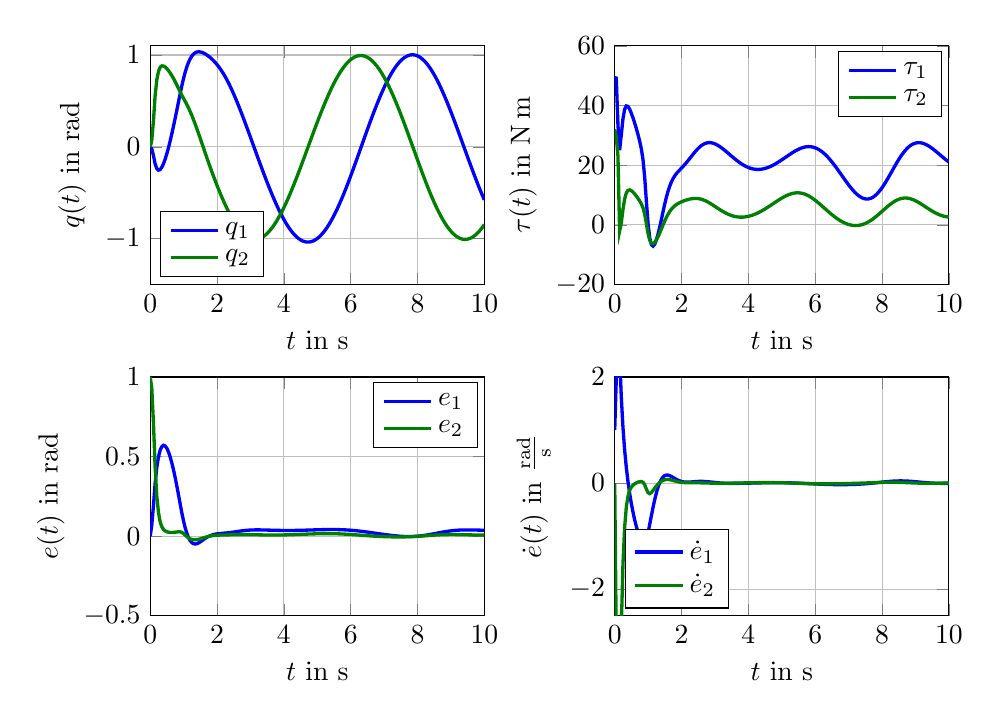
\begin{tikzpicture}

\begin{axis}[%
width=0.35\textwidth,
height=0.25\textwidth,
scale only axis,
xmin=0,
xmax=10,
xlabel={$t$ in $\mathrm{s}$},
xmajorgrids,
ymin=-1.5,
ymax=1.1,
ylabel={$q(t)$ in $\mathrm{rad}$},
ymajorgrids,
name=plot1,
legend style={at={(0.03,0.03)},anchor=south west,draw=black,fill=white,legend cell align=left}
]
\addplot [
color=blue,
solid,
line width=1.2pt
]
table[row sep=crcr]{
0 0\\
0.0464369793164942 -0.0231232507690205\\
0.0964369793164943 -0.0950891756447007\\
0.146436979316494 -0.185815703158844\\
0.196436979316494 -0.236681293585064\\
0.246436979316494 -0.254161066250717\\
0.296436979316494 -0.247563136889258\\
0.346436979316494 -0.222968959459308\\
0.396436979316495 -0.184406589001388\\
0.446436979316495 -0.134642626731092\\
0.496436979316495 -0.0756644948235512\\
0.546436979316495 -0.00899385504290011\\
0.596436979316495 0.0641168612059941\\
0.646436979316495 0.142573316149365\\
0.696436979316495 0.225380472466428\\
0.746436979316495 0.311603026678595\\
0.796436979316495 0.400299724741515\\
0.846436979316495 0.490329319738245\\
0.896436979316495 0.579845231027341\\
0.946436979316495 0.665733991761122\\
0.996436979316495 0.74443611015082\\
1.04643697931649 0.813649079397377\\
1.09643697931648 0.872528650171776\\
1.14643697931648 0.921081900905899\\
1.19643697931647 0.959764765381421\\
1.24643697931647 0.989300914218731\\
1.29643697931646 1.01058911675265\\
1.34643697931646 1.02463559211008\\
1.39643697931645 1.03249091469449\\
1.44643697931645 1.03518703884663\\
1.49643697931644 1.03367795507675\\
1.54643697931643 1.02879186753793\\
1.59643697931643 1.0212017962694\\
1.64643697931642 1.01141638987853\\
1.69643697931642 0.999787624999967\\
1.74643697931641 0.986529699530718\\
1.79643697931641 0.97174367110804\\
1.8464369793164 0.955443823492806\\
1.8964369793164 0.937583216943003\\
1.94643697931639 0.918076949801051\\
1.99643697931639 0.896822328457884\\
2.04643697931638 0.87371555063599\\
2.09643697931637 0.848664774681743\\
2.14643697931637 0.821599644265157\\
2.19643697931636 0.79247749177409\\
2.24643697931636 0.761286562729098\\
2.29643697931635 0.728046689515617\\
2.34643697931635 0.692807897034239\\
2.39643697931634 0.655647447238508\\
2.44643697931634 0.616665825456533\\
2.49643697931633 0.575982140477049\\
2.54643697931632 0.533729355623294\\
2.59643697931632 0.490049694934161\\
2.64643697931631 0.44509048498598\\
2.69643697931631 0.399000607642637\\
2.7464369793163 0.351927659966767\\
2.7964369793163 0.304015850047812\\
2.84643697931629 0.255404604033221\\
2.89643697931629 0.206227820123072\\
2.94643697931628 0.156613678148801\\
2.99643697931628 0.106684896585908\\
3.04643697931627 0.0565593206892266\\
3.09643697931626 0.00635072466591963\\
3.14643697931626 -0.0438302833707081\\
3.19643697931625 -0.0938753531637709\\
3.24643697931625 -0.143677563496526\\
3.29643697931624 -0.193130735022759\\
3.34643697931624 -0.242128924605756\\
3.39643697931623 -0.290566118847999\\
3.44643697931623 -0.338336124516397\\
3.49643697931622 -0.385332637432862\\
3.54643697931621 -0.431449460124795\\
3.59643697931621 -0.476580832408325\\
3.6464369793162 -0.520621837729653\\
3.6964369793162 -0.563468850628369\\
3.74643697931619 -0.605019995938688\\
3.79643697931619 -0.645175597077337\\
3.84643697931618 -0.683838597871125\\
3.89643697931618 -0.720914948984866\\
3.94643697931617 -0.756313955545983\\
3.99643697931617 -0.789948586736105\\
4.04643697931618 -0.821735750883505\\
4.0964369793162 -0.851596541069387\\
4.14643697931621 -0.87945645668804\\
4.19643697931623 -0.90524560605244\\
4.24643697931625 -0.928898894287159\\
4.29643697931626 -0.950356199639997\\
4.34643697931628 -0.969562540163525\\
4.3964369793163 -0.986468231604335\\
4.44643697931631 -1.00102903637811\\
4.49643697931633 -1.01320630274778\\
4.54643697931635 -1.0229670927746\\
4.59643697931636 -1.03028429727129\\
4.64643697931638 -1.03513673583526\\
4.6964369793164 -1.03750924005423\\
4.74643697931641 -1.03739271813419\\
4.79643697931643 -1.03478419947751\\
4.84643697931645 -1.02968685811874\\
4.89643697931646 -1.02211001438906\\
4.94643697931648 -1.01206911470974\\
4.9964369793165 -0.999585689990104\\
5.04643697931651 -0.984687293702144\\
5.09643697931653 -0.967407421292035\\
5.14643697931655 -0.947785413130959\\
5.19643697931656 -0.925866343661791\\
5.24643697931658 -0.901700899716922\\
5.2964369793166 -0.875345251118847\\
5.34643697931661 -0.846860916586832\\
5.39643697931663 -0.816314627628652\\
5.44643697931665 -0.783778192483036\\
5.49643697931666 -0.749328361307422\\
5.54643697931668 -0.713046692718213\\
5.5964369793167 -0.675019420560367\\
5.64643697931671 -0.635337318513908\\
5.69643697931673 -0.594095558965655\\
5.74643697931675 -0.551393561626342\\
5.79643697931676 -0.507334826794528\\
5.84643697931678 -0.462026748073673\\
5.8964369793168 -0.415580399808382\\
5.94643697931681 -0.368110295529473\\
5.99643697931683 -0.319734115222153\\
6.04643697931685 -0.270572401121931\\
6.09643697931686 -0.220748223802878\\
6.14643697931688 -0.170386822320665\\
6.1964369793169 -0.119615223874224\\
6.24643697931691 -0.068561849654775\\
6.29643697931693 -0.0173561141266611\\
6.34643697931695 0.0338719751134363\\
6.39643697931696 0.0849922104735049\\
6.44643697931698 0.135874565286077\\
6.496436979317 0.186389558811594\\
6.54643697931702 0.236408603231481\\
6.59643697931703 0.28580433203798\\
6.64643697931705 0.334450910470404\\
6.69643697931707 0.382224329539096\\
6.74643697931708 0.429002685691323\\
6.7964369793171 0.47466644833736\\
6.84643697931712 0.519098717342315\\
6.89643697931713 0.562185472294242\\
6.94643697931715 0.603815814980765\\
6.99643697931717 0.643882206132585\\
7.04643697931718 0.68228069719045\\
7.0964369793172 0.718911157665165\\
7.14643697931722 0.753677498606354\\
7.19643697931723 0.786487892771713\\
7.24643697931725 0.817254992274148\\
7.29643697931727 0.845896144746698\\
7.34643697931728 0.872333609362417\\
7.3964369793173 0.896494774330672\\
7.44643697931732 0.918312377709686\\
7.49643697931733 0.937724733472216\\
7.54643697931735 0.954675964679573\\
7.59643697931737 0.969116245302746\\
7.64643697931738 0.981002051627411\\
7.6964369793174 0.99029642325283\\
7.74643697931742 0.996969232424321\\
7.79643697931743 1.00099745883658\\
7.84643697931745 1.00236546516341\\
7.89643697931747 1.00106526651121\\
7.94643697931748 0.997096784916821\\
7.9964369793175 0.990468078122629\\
8.04643697931748 0.981195530408551\\
8.09643697931745 0.969303992493415\\
8.14643697931742 0.954826857659209\\
8.19643697931739 0.937806062445598\\
8.24643697931736 0.918292002535312\\
8.29643697931734 0.89634335768369\\
8.34643697931731 0.872026823471585\\
8.39643697931728 0.845416751898664\\
8.44643697931725 0.816594706949227\\
8.49643697931723 0.785648944847202\\
8.5464369793172 0.752673831466892\\
8.59643697931717 0.717769211136877\\
8.64643697931714 0.681039741896722\\
8.69643697931711 0.642594212319254\\
8.74643697931709 0.602544854561199\\
8.79643697931706 0.561006667625525\\
8.84643697931703 0.518096764115434\\
8.896436979317 0.473933753116915\\
8.94643697931698 0.428637171208226\\
8.99643697931695 0.382326972782712\\
9.04643697931692 0.33512308963576\\
9.09643697931689 0.287145067855584\\
9.14643697931687 0.238511787294915\\
9.19643697931684 0.189341265252816\\
9.24643697931681 0.139750541614132\\
9.29643697931678 0.0898556379196871\\
9.34643697931675 0.0397715781669177\\
9.39643697931673 -0.0103875448618542\\
9.4464369793167 -0.0605084767342622\\
9.49643697931667 -0.110478702118788\\
9.54643697931664 -0.160186358648286\\
9.59643697931662 -0.209520180987318\\
9.64643697931659 -0.258369488362311\\
9.69643697931656 -0.306624224069419\\
9.74643697931653 -0.354175050429999\\
9.79643697931651 -0.400913497917459\\
9.84643697931648 -0.446732163224301\\
9.89643697931645 -0.491524948195499\\
9.94643697931642 -0.535187329949283\\
9.99643697931639 -0.577616652082588\\
};
\addlegendentry{$q_1$};

\addplot [
color=green!50!black,
solid,
line width=1.2pt
]
table[row sep=crcr]{
0 0\\
0.0464369793164942 0.0693172506048697\\
0.0964369793164943 0.284470689110996\\
0.146436979316494 0.556411492665137\\
0.196436979316494 0.728738595279007\\
0.246436979316494 0.82179786751635\\
0.296436979316494 0.86602536422048\\
0.346436979316494 0.881570004997053\\
0.396436979316495 0.880471306378443\\
0.446436979316495 0.869438182524294\\
0.496436979316495 0.852001646178837\\
0.546436979316495 0.829961166843892\\
0.596436979316495 0.804249230089217\\
0.646436979316495 0.775395042371098\\
0.696436979316495 0.743755140187521\\
0.746436979316495 0.709632454426678\\
0.796436979316495 0.67337669517359\\
0.846436979316495 0.63558634255208\\
0.896436979316495 0.59754011335532\\
0.946436979316495 0.561236350864526\\
0.996436979316495 0.527473016485935\\
1.04643697931649 0.49457059015312\\
1.09643697931648 0.460270154776945\\
1.14643697931648 0.423233500071846\\
1.19643697931647 0.383058409304898\\
1.24643697931647 0.339864849590333\\
1.29643697931646 0.293981742062684\\
1.34643697931646 0.245798525711649\\
1.39643697931645 0.195721148860845\\
1.44643697931645 0.144170372784818\\
1.49643697931644 0.0915821900427514\\
1.54643697931643 0.0383934921594169\\
1.59643697931643 -0.0149842056720554\\
1.64643697931642 -0.0681906024083448\\
1.69643697931642 -0.120931733387924\\
1.74643697931641 -0.172981678346181\\
1.79643697931641 -0.224174159901375\\
1.8464369793164 -0.27438925357479\\
1.8964369793164 -0.323539455838131\\
1.94643697931639 -0.371557486172208\\
1.99643697931639 -0.418386657235904\\
2.04643697931638 -0.463973777182896\\
2.09643697931637 -0.508264220266776\\
2.14643697931637 -0.551198768452141\\
2.19643697931636 -0.592711893851116\\
2.24643697931636 -0.632731218360771\\
2.29643697931635 -0.671177922826974\\
2.34643697931635 -0.707967889095597\\
2.39643697931634 -0.743013359553173\\
2.44643697931634 -0.776224902340114\\
2.49643697931633 -0.807513482972217\\
2.54643697931632 -0.83679246712646\\
2.59643697931632 -0.863979414526844\\
2.64643697931631 -0.888997567469619\\
2.69643697931631 -0.911776984627037\\
2.7464369793163 -0.932255315184463\\
2.7964369793163 -0.950378244300643\\
2.84643697931629 -0.966099664547695\\
2.89643697931629 -0.979381638480547\\
2.94643697931628 -0.990194216614547\\
2.99643697931628 -0.99851516641566\\
3.04643697931627 -1.0043296554877\\
3.09643697931626 -1.00762991945891\\
3.14643697931626 -1.00841493441298\\
3.19643697931625 -1.00669010603434\\
3.24643697931625 -1.00246698281321\\
3.29643697931624 -0.995762997897246\\
3.34643697931624 -0.986601242506293\\
3.39643697931623 -0.975010272424118\\
3.44643697931623 -0.961023947475136\\
3.49643697931622 -0.944681301985353\\
3.54643697931621 -0.926026442194231\\
3.59643697931621 -0.905108464739144\\
3.6464369793162 -0.881981388980077\\
3.6964369793162 -0.856704095269137\\
3.74643697931619 -0.829340261354753\\
3.79643697931619 -0.799958289868273\\
3.84643697931618 -0.768631221101417\\
3.89643697931618 -0.73543662683275\\
3.94643697931617 -0.700456482587606\\
3.99643697931617 -0.663777017239999\\
4.04643697931618 -0.625488540160446\\
4.0964369793162 -0.585685247109623\\
4.14643697931621 -0.544465006755211\\
4.19643697931623 -0.50192913006858\\
4.24643697931625 -0.458182124987148\\
4.29643697931626 -0.413331438668565\\
4.34643697931628 -0.367487189479747\\
4.3964369793163 -0.320761890617161\\
4.44643697931631 -0.273270166995071\\
4.49643697931633 -0.225128466803488\\
4.54643697931635 -0.176454768951955\\
4.59643697931636 -0.127368287491492\\
4.64643697931638 -0.0779891740466562\\
4.6964369793164 -0.0284382192858973\\
4.74643697931641 0.0211634455022847\\
4.79643697931643 0.0706946455951102\\
4.84643697931645 0.120034457580875\\
4.89643697931646 0.169062500406684\\
4.94643697931648 0.21765922145094\\
4.9964369793165 0.265706176373351\\
5.04643697931651 0.313086301588351\\
5.09643697931653 0.359684178370157\\
5.14643697931655 0.405386287829166\\
5.19643697931656 0.450081256292942\\
5.24643697931658 0.49366009096676\\
5.2964369793166 0.536016406118305\\
5.34643697931661 0.577046640403362\\
5.39643697931663 0.616650266295959\\
5.44643697931665 0.654729992878427\\
5.49643697931666 0.691191963457575\\
5.54643697931668 0.725945949580695\\
5.5964369793167 0.758905543015008\\
5.64643697931671 0.789988347120632\\
5.69643697931673 0.819116168794116\\
5.74643697931675 0.846215211799383\\
5.79643697931676 0.871216271855141\\
5.84643697931678 0.894054933336396\\
5.8964369793168 0.91467176689846\\
5.94643697931681 0.933012526770673\\
5.99643697931683 0.949028345918286\\
6.04643697931685 0.962675926758073\\
6.09643697931686 0.973917724659381\\
6.14643697931688 0.9827221210917\\
6.1964369793169 0.989063583018011\\
6.24643697931691 0.992922805006035\\
6.29643697931693 0.994286830560684\\
6.34643697931695 0.993149149387021\\
6.39643697931696 0.989509767679492\\
6.44643697931698 0.983375249090264\\
6.496436979317 0.974758724731053\\
6.54643697931702 0.963679871367436\\
6.59643697931703 0.950164857820124\\
6.64643697931705 0.934246260437268\\
6.69643697931707 0.9159629492913\\
6.74643697931708 0.89535994743753\\
6.7964369793171 0.872488266117081\\
6.84643697931712 0.847404719176081\\
6.89643697931713 0.820171720202628\\
6.94643697931715 0.790857065960821\\
6.99643697931717 0.759533709642706\\
7.04643697931718 0.726279527284171\\
7.0964369793172 0.691177080419917\\
7.14643697931722 0.654313377704633\\
7.19643697931723 0.615779637818978\\
7.24643697931725 0.575671055523719\\
7.29643697931727 0.534086572236025\\
7.34643697931728 0.491128651990168\\
7.3964369793173 0.446903063123204\\
7.44643697931732 0.401518665508286\\
7.49643697931733 0.355087202658542\\
7.54643697931735 0.307723097557881\\
7.59643697931737 0.259543250654676\\
7.64643697931738 0.210666838089651\\
7.6964369793174 0.161215107923839\\
7.74643697931742 0.111311171882608\\
7.79643697931743 0.06107978992632\\
7.84643697931745 0.0106471447815952\\
7.89643697931747 -0.0398593965956213\\
7.94643697931748 -0.0903115378087066\\
7.9964369793175 -0.140580327377405\\
8.04643697931748 -0.190536456048944\\
8.09643697931745 -0.240050580376547\\
8.14643697931742 -0.288993675556119\\
8.19643697931739 -0.337237419813378\\
8.24643697931736 -0.38465461144539\\
8.29643697931734 -0.431119617877228\\
8.34643697931731 -0.476508853821\\
8.39643697931728 -0.52070128296285\\
8.44643697931725 -0.5635789348185\\
8.49643697931723 -0.605027425849428\\
8.5464369793172 -0.644936472016171\\
8.59643697931717 -0.683200379015953\\
8.64643697931714 -0.719718496740505\\
8.69643697931711 -0.754395626048826\\
8.74643697931709 -0.787142368631538\\
8.79643697931706 -0.817875414225765\\
8.84643697931703 -0.846517763283693\\
8.896436979317 -0.872998886930171\\
8.94643697931698 -0.897254829237416\\
8.99643697931695 -0.91922825918219\\
9.04643697931692 -0.9388684809684\\
9.09643697931689 -0.956131411691941\\
9.14643697931687 -0.970979534733677\\
9.19643697931684 -0.983381836033689\\
9.24643697931681 -0.993313728822022\\
9.29643697931678 -1.00075697075457\\
9.34643697931675 -1.00569957597527\\
9.39643697931673 -1.00813572356077\\
9.4464369793167 -1.00806566316274\\
9.49643697931667 -1.00549561840767\\
9.54643697931664 -1.00043768863159\\
9.59643697931662 -0.992909749662943\\
9.64643697931659 -0.982935354467607\\
9.69643697931656 -0.970543634421592\\
9.74643697931653 -0.955769201720253\\
9.79643697931651 -0.938652052979143\\
9.84643697931648 -0.919237473492241\\
9.89643697931645 -0.897575940984731\\
9.94643697931642 -0.873723027131778\\
9.99643697931639 -0.847739294698357\\
};
\addlegendentry{$q_2$};

\end{axis}

\begin{axis}[%
width=0.35\textwidth,
height=0.25\textwidth,
scale only axis,
xmin=0,
xmax=10,
xlabel={$t$ in $\mathrm{s}$},
xmajorgrids,
ymin=-0.5,
ymax=1,
ylabel={$e(t)$ in $\mathrm{rad}$},
ymajorgrids,
name=plot3,
at=(plot1.below south west),
anchor=above north west,
legend style={draw=black,fill=white,legend cell align=left}
]
\addplot [
color=blue,
solid,
line width=1.2pt
]
table[row sep=crcr]{
0 0\\
0.0464369793164942 0.0695435424883056\\
0.0964369793164943 0.191376745673877\\
0.146436979316494 0.331729882718435\\
0.196436979316494 0.431857373216807\\
0.246436979316494 0.49811120740127\\
0.296436979316494 0.539677591252522\\
0.346436979316494 0.562517593029642\\
0.396436979316495 0.570540707028376\\
0.446436979316495 0.566397095014427\\
0.496436979316495 0.551960152045907\\
0.546436979316495 0.528640210111203\\
0.596436979316495 0.497581346447175\\
0.646436979316495 0.45977279109631\\
0.696436979316495 0.416107982799426\\
0.746436979316495 0.367424389550003\\
0.796436979316495 0.314569437539899\\
0.846436979316495 0.258594787986943\\
0.896436979316495 0.201261901904443\\
0.946436979316495 0.145603805337661\\
0.996436979316495 0.0951044291587709\\
1.04643697931649 0.0519957879990063\\
1.09643697931648 0.0170568839620403\\
1.14643697931648 -0.00977920058279302\\
1.19643697931647 -0.0290226810225607\\
1.24643697931647 -0.0414458163139051\\
1.29643697931646 -0.0479901494132295\\
1.34643697931646 -0.0496987514425646\\
1.39643697931645 -0.0476530350632483\\
1.44643697931645 -0.0429097020570918\\
1.49643697931644 -0.0364413377028384\\
1.54643697931643 -0.0290885417722879\\
1.59643697931643 -0.0215304997910171\\
1.64643697931642 -0.0142757803098565\\
1.69643697931642 -0.00767003456412896\\
1.74643697931641 -0.00191490551895368\\
1.79643697931641 0.00290730227209468\\
1.8464369793164 0.0068072094106636\\
1.8964369793164 0.00986274903219375\\
1.94643697931639 0.0121958277512564\\
1.99643697931639 0.0139520632043513\\
2.04643697931638 0.0152839934791514\\
2.09643697931637 0.0163378860080293\\
2.14643697931637 0.0172440768321996\\
2.19643697931636 0.0181106172894738\\
2.24643697931636 0.0190198861741409\\
2.29643697931635 0.0200277394807817\\
2.34643697931635 0.0211647155724597\\
2.39643697931634 0.022438789276724\\
2.44643697931634 0.0238391725164298\\
2.49643697931633 0.0253406900272669\\
2.54643697931632 0.026908313498991\\
2.59643697931632 0.0285015106077416\\
2.64643697931631 0.0300781490179338\\
2.69643697931631 0.0315977807013181\\
2.7464369793163 0.0330242109976758\\
2.7964369793163 0.034327324338767\\
2.84643697931629 0.0354841920452463\\
2.89643697931629 0.0364795271490443\\
2.94643697931628 0.0373055783483263\\
2.99643697931628 0.0379615719861854\\
3.04643697931627 0.0384528191168266\\
3.09643697931626 0.0387896055059443\\
3.14643697931626 0.0389859765915827\\
3.19643697931625 0.0390585176777377\\
3.24643697931625 0.0390252128442441\\
3.29643697931624 0.0389044455789687\\
3.34643697931624 0.0387141817745669\\
3.39643697931623 0.0384713535501396\\
3.44643697931623 0.0381914423766952\\
3.49643697931622 0.0378882438443394\\
3.54643697931621 0.0375737851258797\\
3.59643697931621 0.0372583600600282\\
3.6464369793162 0.0369506454181232\\
3.6964369793162 0.0366578644432985\\
3.74643697931619 0.0363859689876808\\
3.79643697931619 0.0361398182888943\\
3.84643697931618 0.0359233395125149\\
3.89643697931618 0.0357396617742416\\
3.94643697931617 0.0355912208689784\\
3.99643697931617 0.0354798360842673\\
4.04643697931618 0.0354067632137217\\
4.0964369793162 0.0353727293386127\\
4.14643697931621 0.0353779553444585\\
4.19643697931623 0.0354221717618273\\
4.24643697931625 0.0355046326399544\\
4.29643697931626 0.0356241310195827\\
4.34643697931628 0.0357790183582013\\
4.3964369793163 0.0359672291135597\\
4.44643697931631 0.0361863106967552\\
4.49643697931633 0.0364334582096781\\
4.54643697931635 0.036705552797629\\
4.59643697931636 0.0369992020703217\\
4.64643697931638 0.0373107808554144\\
4.6964369793164 0.0376364705252438\\
4.74643697931641 0.0379722952562185\\
4.79643697931643 0.0383141538196589\\
4.84643697931645 0.0386578458435846\\
4.89643697931646 0.0389990919093581\\
4.94643697931648 0.0393335473374252\\
4.9964369793165 0.0396568100527104\\
5.04643697931651 0.0399644234782235\\
5.09643697931653 0.0402518759549898\\
5.14643697931655 0.0405145986908588\\
5.19643697931656 0.0407479646572313\\
5.24643697931658 0.0409472911346747\\
5.2964369793166 0.0411078487085558\\
5.34643697931661 0.0412248793920834\\
5.39643697931663 0.041293626175297\\
5.44643697931665 0.041309375651575\\
5.49643697931666 0.0412675144696483\\
5.54643697931668 0.0411635992402623\\
5.5964369793167 0.0409934382659845\\
5.64643697931671 0.0407531821644825\\
5.69643697931673 0.0404394192486282\\
5.74643697931675 0.0400492705524639\\
5.79643697931676 0.0395804787885261\\
5.84643697931678 0.0390314854038061\\
5.8964369793168 0.0384014903396526\\
5.94643697931681 0.0376904901045746\\
5.99643697931683 0.0368992912753394\\
6.04643697931685 0.0360294984155417\\
6.09643697931686 0.0350834774460966\\
6.14643697931688 0.0340642974870534\\
6.1964369793169 0.0329756558804671\\
6.24643697931691 0.0318217922998434\\
6.29643697931693 0.0306073984200898\\
6.34643697931695 0.0293375295187546\\
6.39643697931696 0.0280175236547414\\
6.44643697931698 0.0266529328572355\\
6.496436979317 0.0252494692441115\\
6.54643697931702 0.0238129673859527\\
6.59643697931703 0.022349362735411\\
6.64643697931705 0.0208646847053537\\
6.69643697931707 0.0193650620958723\\
6.74643697931708 0.0178567380674807\\
6.7964369793171 0.0163460917057701\\
6.84643697931712 0.0148396633494204\\
6.89643697931713 0.0133441811641016\\
6.94643697931715 0.0118665868405897\\
6.99643697931717 0.0104140586884224\\
7.04643697931718 0.00899403071906435\\
7.0964369793172 0.00761420652200084\\
7.14643697931722 0.0062825668150881\\
7.19643697931723 0.00500736950000336\\
7.24643697931725 0.00379714089492511\\
7.29643697931727 0.00266065658249348\\
7.34643697931728 0.00160691004340663\\
7.3964369793173 0.000645066992692733\\
7.44643697931732 -0.000215596850692723\\
7.49643697931733 -0.000965776894182979\\
7.54643697931735 -0.0015962419193124\\
7.59643697931737 -0.00209795931283596\\
7.64643697931738 -0.00246224450944077\\
7.6964369793174 -0.00268093491091526\\
7.74643697931742 -0.00274658723911492\\
7.79643697931743 -0.00265269563990589\\
7.84643697931745 -0.00239392593535193\\
7.89643697931747 -0.00196635932473421\\
7.94643697931748 -0.00136773671924395\\
7.9964369793175 -0.00059769296878065\\
8.04643697931748 0.000342031253221076\\
8.09643697931745 0.00144741294700967\\
8.14643697931742 0.00271201860382875\\
8.19643697931739 0.00412693612600468\\
8.24643697931736 0.00568077639765174\\
8.29643697931734 0.00735975085902685\\
8.34643697931731 0.00914782754901067\\
8.39643697931728 0.0110269638791491\\
8.44643697931725 0.0129774103236262\\
8.49643697931723 0.0149780756603183\\
8.5464369793172 0.0170069416825204\\
8.59643697931717 0.0190415135635545\\
8.64643697931714 0.0210592912665878\\
8.69643697931711 0.0230382473701349\\
8.74643697931709 0.0249572971597306\\
8.79643697931706 0.0267967475444489\\
8.84643697931703 0.0285387120877619\\
8.896436979317 0.0301674801112483\\
8.94643697931698 0.0316698284926843\\
8.99643697931695 0.0330352656149444\\
9.04643697931692 0.0342561981791219\\
9.09643697931689 0.0353280135260016\\
9.14643697931687 0.0362490728906553\\
9.19643697931684 0.0370206146789666\\
9.24643697931681 0.0376465712510213\\
9.29643697931678 0.038133307483305\\
9.34643697931675 0.0384892940657605\\
9.39643697931673 0.0387247325011114\\
9.4464369793167 0.0388511515687224\\
9.49643697931667 0.0388809961824478\\
9.54643697931664 0.0388272289186219\\
9.59643697931662 0.0387029620860405\\
9.64643697931659 0.0385211343767855\\
9.69643697931656 0.0382942413897995\\
9.74643697931653 0.0380341242694297\\
9.79643697931651 0.0377518159483283\\
9.84643697931648 0.0374574405205834\\
9.89643697931645 0.0371601584177984\\
9.94643697931642 0.0368681484434323\\
9.99643697931639 0.0365886172827389\\
};
\addlegendentry{$e_1$};

\addplot [
color=green!50!black,
solid,
line width=1.2pt
]
table[row sep=crcr]{
0 1\\
0.0464369793164942 0.929604746608474\\
0.0964369793164943 0.710882868102659\\
0.146436979316494 0.432885759025906\\
0.196436979316494 0.252029622976246\\
0.246436979316494 0.147989907531689\\
0.296436979316494 0.090358003238434\\
0.346436979316494 0.0590184945289187\\
0.396436979316495 0.0419713438147927\\
0.446436979316495 0.0325529921095676\\
0.496436979316495 0.0272835447069899\\
0.546436979316495 0.0244202852395595\\
0.596436979316495 0.0230929745149102\\
0.646436979316495 0.0228399901136845\\
0.696436979316495 0.0233775483094748\\
0.746436979316495 0.0244804578762686\\
0.796436979316495 0.0258815409731641\\
0.846436979316495 0.0270694360147652\\
0.896436979316495 0.0268569132896569\\
0.946436979316495 0.0233412564716557\\
0.996436979316495 0.0158240319652434\\
1.04643697931649 0.00608793973556476\\
1.09643697931648 -0.00350152903755357\\
1.14643697931648 -0.0114964621655936\\
1.19643697931647 -0.0173820873980462\\
1.24643697931647 -0.0211632440471007\\
1.29643697931646 -0.0230514409203426\\
1.34643697931646 -0.023316713625281\\
1.39643697931645 -0.0222439144943771\\
1.44643697931645 -0.0201313188789702\\
1.49643697931644 -0.0172913496339976\\
1.54643697931643 -0.0140365536588572\\
1.59643697931643 -0.0106536373969818\\
1.64643697931642 -0.00737794097454739\\
1.69643697931642 -0.00437862830570242\\
1.74643697931641 -0.00175729101432057\\
1.79643697931641 0.000443339295102874\\
1.8464369793164 0.00222579225750463\\
1.8964369793164 0.00362362072313505\\
1.94643697931639 0.00468890023834134\\
1.99643697931639 0.00548230088653612\\
2.04643697931638 0.00606569627246789\\
2.09643697931637 0.00649694652364496\\
2.14643697931637 0.0068264587453194\\
2.19643697931636 0.00709519545125303\\
2.24643697931636 0.00733386803058456\\
2.29643697931635 0.00756308824164609\\
2.34643697931635 0.00779426173766518\\
2.39643697931634 0.00803100884765529\\
2.44643697931634 0.00827090139236553\\
2.49643697931633 0.00850731684189387\\
2.54643697931632 0.0087312351145209\\
2.59643697931632 0.00893283846736437\\
2.64643697931631 0.00910281850309957\\
2.69643697931631 0.00923334138556553\\
2.7464369793163 0.00931866674049986\\
2.7964369793163 0.00935545161918327\\
2.84643697931629 0.00934279453524467\\
2.89643697931629 0.00928208504279149\\
2.94643697931628 0.00917672341699916\\
2.99643697931628 0.00903176628727842\\
3.04643697931627 0.00885354161581142\\
3.09643697931626 0.00864926369426\\
3.14643697931626 0.00842666813590354\\
3.19643697931625 0.00819367912671554\\
3.24643697931625 0.00795811633541499\\
3.29643697931624 0.00772744608526776\\
3.34643697931624 0.00750857968069396\\
3.39643697931623 0.00730772034036109\\
3.44643697931623 0.00713025854368177\\
3.49643697931622 0.00698071365030051\\
3.54643697931621 0.00686271758139112\\
3.59643697931621 0.00677903446883421\\
3.6464369793162 0.00673160878704904\\
3.6964369793162 0.00672163378259971\\
3.74643697931619 0.00674963206611279\\
3.79643697931619 0.00681554095383308\\
3.84643697931618 0.00691879637270398\\
3.89643697931618 0.00705841065942336\\
3.94643697931617 0.00723304117805612\\
3.99643697931617 0.00744104817396063\\
4.04643697931618 0.00768054154743436\\
4.0964369793162 0.00794941719798836\\
4.14643697931621 0.00824538424072785\\
4.19643697931623 0.00856598474975562\\
4.24643697931625 0.00890860778872116\\
4.29643697931626 0.00927049940640723\\
4.34643697931628 0.0096487700711454\\
4.3964369793163 0.0100404007519911\\
4.44643697931631 0.0104422485773728\\
4.49643697931633 0.0108510527511721\\
4.54643697931635 0.0112634412066332\\
4.59643697931636 0.0116759383425467\\
4.64643697931638 0.0120849741155492\\
4.6964369793164 0.0124868947502129\\
4.74643697931641 0.0128779753615036\\
4.79643697931643 0.0132544348444205\\
4.84643697931645 0.0136124534531348\\
4.89643697931646 0.013948193546186\\
4.94643697931648 0.0142578239960345\\
4.9964369793165 0.0145375487341717\\
5.04643697931651 0.0147836398150621\\
5.09643697931653 0.0149924752270024\\
5.14643697931655 0.0151605814555745\\
5.19643697931656 0.0152846805227433\\
5.24643697931658 0.0153617408957248\\
5.2964369793166 0.015389031304768\\
5.34643697931661 0.0153641761531412\\
5.39643697931663 0.0152852108741709\\
5.44643697931665 0.0151506353180371\\
5.49643697931666 0.0149594630618189\\
5.54643697931668 0.0147112644518823\\
5.5964369793167 0.0144062012224915\\
5.64643697931671 0.0140450506941653\\
5.69643697931673 0.0136292178359388\\
5.74643697931675 0.013160733864768\\
5.79643697931676 0.0126422405332839\\
5.84643697931678 0.0120769597999457\\
5.8964369793168 0.011468649157324\\
5.94643697931681 0.0108215434890165\\
5.99643697931683 0.0101402849089396\\
6.04643697931685 0.00942984258498603\\
6.09643697931686 0.00869542503905085\\
6.14643697931688 0.00794238782289169\\
6.1964369793169 0.00717613976855591\\
6.24643697931691 0.00640205117715675\\
6.29643697931693 0.00562536731699737\\
6.34643697931695 0.00485113043465968\\
6.39643697931696 0.00408411313513068\\
6.44643697931698 0.003328765468953\\
6.496436979317 0.00258917740187603\\
6.54643697931702 0.00186905757681854\\
6.59643697931703 0.00117172846125457\\
6.64643697931705 0.000500137162047332\\
6.69643697931707 -0.000143119561534455\\
6.74643697931708 -0.000755758201893775\\
6.7964369793171 -0.00133576194780916\\
6.84643697931712 -0.00188132764614324\\
6.89643697931713 -0.00239080945078163\\
6.94643697931715 -0.00286266237188204\\
6.99643697931717 -0.00329538884609459\\
7.04643697931718 -0.00368749124057732\\
7.0964369793172 -0.00403743290079217\\
7.14643697931722 -0.00434360997336658\\
7.19643697931723 -0.00460433579718744\\
7.24643697931725 -0.00481783917251466\\
7.29643697931727 -0.00498227730167877\\
7.34643697931728 -0.00509576365782605\\
7.3964369793173 -0.0051564104926633\\
7.44643697931732 -0.00516238515391398\\
7.49643697931733 -0.0051119788628653\\
7.54643697931735 -0.00500368611681518\\
7.59643697931737 -0.00483629244360312\\
7.64643697931738 -0.00460896785527945\\
7.6964369793174 -0.00432136302889069\\
7.74643697931742 -0.00397370498063754\\
7.79643697931743 -0.00356688878431075\\
7.84643697931745 -0.00310256170026222\\
7.89643697931747 -0.00258319591228241\\
7.94643697931748 -0.00201214591083886\\
7.9964369793175 -0.00139368642572774\\
8.04643697931748 -0.000733026741866233\\
8.09643697931745 -3.62973061806826e-05\\
8.14643697931742 0.000689495140850926\\
8.19643697931739 0.00143654697069212\\
8.24643697931736 0.00219637347567891\\
8.29643697931734 0.00295996119501452\\
8.34643697931731 0.00371795458674923\\
8.39643697931728 0.00446087219990676\\
8.44643697931725 0.00517934470096126\\
8.49643697931723 0.00586436454370032\\
8.5464369793172 0.00650753513742808\\
8.59643697931717 0.0071013064190264\\
8.64643697931714 0.0076391840012946\\
8.69643697931711 0.00811590060544121\\
8.74643697931709 0.00852754114261611\\
8.79643697931706 0.008871616265264\\
8.84643697931703 0.00914708302547806\\
8.896436979317 0.00935431498066597\\
8.94643697931698 0.00949502724909301\\
8.99643697931695 0.00957216432365049\\
9.04643697931692 0.00958975973705134\\
9.09643697931689 0.00955277693185708\\
9.14643697931687 0.00946694006313165\\
9.19643697931684 0.00933856219327589\\
9.24643697931681 0.00917437672440979\\
9.29643697931678 0.00898137625013506\\
9.34643697931675 0.00876666154351735\\
9.39643697931673 0.00853730229516225\\
9.4464369793167 0.00830021053564256\\
9.49643697931667 0.008062027382853\\
9.54643697931664 0.00782902373325745\\
9.59643697931662 0.00760701561272537\\
9.64643697931659 0.00740129496488817\\
9.69643697931656 0.00721657656680774\\
9.74643697931653 0.00705696146700485\\
9.79643697931651 0.00692591684827704\\
9.84643697931648 0.00682627159049098\\
9.89643697931645 0.00676022614228056\\
9.94643697931642 0.00672937470787494\\
9.99643697931639 0.00673473730249274\\
};
\addlegendentry{$e_2$};

\end{axis}

\begin{axis}[%
width=0.35\textwidth,
height=0.25\textwidth,
scale only axis,
xmin=0,
xmax=10,
xlabel={$t$ in $\mathrm{s}$},
xmajorgrids,
ymin=-2.5,
ymax=2,
ylabel={$\dot{e}(t)$ in $\mathrm{\frac{rad}{s}}$},
ymajorgrids,
name=plot2,
at=(plot3.right of south east),
anchor=left of south west,
legend style={at={(0.03,0.03)},anchor=south west,draw=black,fill=white,legend cell align=left}
]
\addplot [
color=blue,
solid,
line width=1.2pt
]
table[row sep=crcr]{
0 1\\
0.0464369793164942 1.9543649554283\\
0.0964369793164943 2.91372628955995\\
0.146436979316494 2.41999768792638\\
0.196436979316494 1.62669419121449\\
0.246436979316494 1.05380978536805\\
0.296436979316494 0.628285956916101\\
0.346436979316494 0.298093972338239\\
0.396436979316495 0.031510014220528\\
0.446436979316495 -0.191112669803544\\
0.496436979316495 -0.381728123334603\\
0.546436979316495 -0.547291464295427\\
0.596436979316495 -0.691783832252472\\
0.646436979316495 -0.817591699633676\\
0.696436979316495 -0.926226876016425\\
0.746436979316495 -1.01834626797454\\
0.796436979316495 -1.0925106291588\\
0.846436979316495 -1.14088854464935\\
0.896436979316495 -1.14205323900903\\
0.946436979316495 -1.07186986917487\\
0.996436979316495 -0.940705222197213\\
1.04643697931649 -0.781289050486597\\
1.09643697931648 -0.616616965622196\\
1.14643697931648 -0.458580687663343\\
1.19643697931647 -0.313761035466322\\
1.24643697931647 -0.186324672139147\\
1.29643697931646 -0.0789464414915215\\
1.34643697931646 0.00697644647678383\\
1.39643697931645 0.0713096412461443\\
1.44643697931645 0.115165404819919\\
1.49643697931644 0.140757279009657\\
1.54643697931643 0.151087723995713\\
1.59643697931643 0.149541586848261\\
1.64643697931642 0.139501592675121\\
1.69643697931642 0.124064507681681\\
1.74643697931641 0.105875227358413\\
1.79643697931641 0.0870570906422168\\
1.8464369793164 0.0692067879216722\\
1.8964369793164 0.053427924275429\\
1.94643697931639 0.0403862190383165\\
1.99643697931639 0.0303760528115292\\
2.04643697931638 0.0233919256483417\\
2.09643697931637 0.0192003302027217\\
2.14643697931637 0.017408582543618\\
2.19643697931636 0.0175278919512083\\
2.24643697931636 0.019028624017803\\
2.29643697931635 0.0213863606215448\\
2.34643697931635 0.0241179762846807\\
2.39643697931634 0.0268075330662967\\
2.44643697931634 0.0291223511509274\\
2.49643697931633 0.0308201261825892\\
2.54643697931632 0.0317483953428147\\
2.59643697931632 0.0318379486611409\\
2.64643697931631 0.0310919034102947\\
2.69643697931631 0.029572107806086\\
2.7464369793163 0.027384352747183\\
2.7964369793163 0.0246636048258743\\
2.84643697931629 0.0215601874743087\\
2.89643697931629 0.0182275706444832\\
2.94643697931628 0.0148122017791377\\
2.99643697931628 0.0114456226312573\\
3.04643697931627 0.00823895830870136\\
3.09643697931626 0.00527972599042659\\
3.14643697931626 0.00263078516087267\\
3.19643697931625 0.00033114027460468\\
3.24643697931625 -0.00160178212596673\\
3.29643697931624 -0.00316881688722026\\
3.34643697931624 -0.00438515681430951\\
3.39643697931623 -0.00527629026867293\\
3.44643697931623 -0.00587414556551602\\
3.49643697931622 -0.00621371861331987\\
3.54643697931621 -0.00633035772128143\\
3.59643697931621 -0.00625777823163154\\
3.6464369793162 -0.00602679172800213\\
3.6964369793162 -0.00566466805383936\\
3.74643697931619 -0.00519500661182015\\
3.79643697931619 -0.00463797558254453\\
3.84643697931618 -0.00401077991949561\\
3.89643697931618 -0.00332823569311758\\
3.94643697931617 -0.0026033536230855\\
3.99643697931617 -0.00184786309005491\\
4.04643697931618 -0.00107263536241942\\
4.0964369793162 -0.000287988410317519\\
4.14643697931621 0.000496125959027482\\
4.19643697931623 0.00127003918749141\\
4.24643697931625 0.00202436632151981\\
4.29643697931626 0.00275006553611529\\
4.34643697931628 0.0034385328539801\\
4.3964369793163 0.00408171042752692\\
4.44643697931631 0.00467219038038141\\
4.49643697931633 0.00520330039618583\\
4.54643697931635 0.00566916148423466\\
4.59643697931636 0.00606471232690112\\
4.64643697931638 0.00638569816292425\\
4.6964369793164 0.00662862523560895\\
4.74643697931641 0.00679068445496957\\
4.79643697931643 0.00686965013498579\\
4.84643697931645 0.00686376151479076\\
4.89643697931646 0.00677159627267285\\
4.94643697931648 0.00659194637180197\\
4.9964369793165 0.00632370727061282\\
5.04643697931651 0.00596579168490247\\
5.09643697931653 0.00551707857471306\\
5.14643697931655 0.00497640671638144\\
5.19643697931656 0.00434262000318214\\
5.24643697931658 0.00361466844822211\\
5.2964369793166 0.0027917647806891\\
5.34643697931661 0.00187359168771384\\
5.39643697931663 0.000860549450295123\\
5.44643697931665 -0.000245971617568008\\
5.49643697931666 -0.00144331434170031\\
5.54643697931668 -0.002727297566261\\
5.5964369793167 -0.00409200472015214\\
5.64643697931671 -0.00552964358279862\\
5.69643697931673 -0.00703049954032453\\
5.74643697931675 -0.0085829985456537\\
5.79643697931676 -0.0101738873227532\\
5.84643697931678 -0.0117885277605427\\
5.8964369793168 -0.0134112909948378\\
5.94643697931681 -0.0150260257431972\\
5.99643697931683 -0.0166165665258912\\
6.04643697931685 -0.0181672418495962\\
6.09643697931686 -0.0196633412503336\\
6.14643697931688 -0.0210915036949222\\
6.1964369793169 -0.0224399979060459\\
6.24643697931691 -0.0236988766644325\\
6.29643697931693 -0.0248600004475921\\
6.34643697931695 -0.02591693900037\\
6.39643697931696 -0.0268647707748717\\
6.44643697931698 -0.0276998081988071\\
6.496436979317 -0.0284192806386192\\
6.54643697931702 -0.0290210066518326\\
6.59643697931703 -0.0295030832731705\\
6.64643697931705 -0.0298636137304\\
6.69643697931707 -0.0301004874390638\\
6.74643697931708 -0.0302112186420591\\
6.7964369793171 -0.0301928436572537\\
6.84643697931712 -0.0300418720264467\\
6.89643697931713 -0.0297542841817882\\
6.94643697931715 -0.0293255674780046\\
6.99643697931717 -0.0287507832488509\\
7.04643697931718 -0.0280246594661782\\
7.0964369793172 -0.0271417061053237\\
7.14643697931722 -0.0260963529845962\\
7.19643697931723 -0.0248831122620405\\
7.24643697931725 -0.0234967696437735\\
7.29643697931727 -0.0219326094727805\\
7.34643697931728 -0.0201866790767356\\
7.3964369793173 -0.0182560969529643\\
7.44643697931732 -0.0161394074826307\\
7.49643697931733 -0.0138369818461633\\
7.54643697931735 -0.0113514606491683\\
7.59643697931737 -0.00868822852034568\\
7.64643697931738 -0.00585590477275472\\
7.6964369793174 -0.0028668274392098\\
7.74643697931742 0.00026249889563662\\
7.79643697931743 0.00351102732207916\\
7.84643697931745 0.00685290549055048\\
7.89643697931747 0.0102573678956276\\
7.94643697931748 0.0136888247494856\\
7.9964369793175 0.0171071824851707\\
8.04643697931748 0.0204684196950287\\
8.09643697931745 0.0237254261848792\\
8.14643697931742 0.0268290928819199\\
8.19643697931739 0.0297296185488009\\
8.24643697931736 0.0323779783547378\\
8.29643697931734 0.034727482358383\\
8.34643697931731 0.0367353415976328\\
8.39643697931728 0.0383641575256776\\
8.44643697931725 0.0395832572772949\\
8.49643697931723 0.0403698113451181\\
8.5464369793172 0.0407096889504167\\
8.59643697931717 0.0405980262176575\\
8.64643697931714 0.0400394998281275\\
8.69643697931711 0.0390483116887129\\
8.74643697931709 0.0376478973417007\\
8.79643697931706 0.0358703730139947\\
8.84643697931703 0.0337557353519624\\
8.896436979317 0.031350826748989\\
8.94643697931698 0.0287080804892437\\
8.99643697931695 0.0258840657385861\\
9.04643697931692 0.0229378634961515\\
9.09643697931689 0.0199293202323779\\
9.14643697931687 0.0169172438394811\\
9.19643697931684 0.013957623327454\\
9.24643697931681 0.011101965527725\\
9.29643697931678 0.00839584535050675\\
9.34643697931675 0.00587775847951422\\
9.39643697931673 0.00357834622544373\\
9.4464369793167 0.00152003321102223\\
9.49643697931667 -0.000282916755803053\\
9.54643697931664 -0.00182395787416767\\
9.59643697931662 -0.003103496431343\\
9.64643697931659 -0.00412788952021648\\
9.69643697931656 -0.00490830844866597\\
9.74643697931653 -0.00545956674145365\\
9.79643697931651 -0.00579900128394295\\
9.84643697931648 -0.0059454755207593\\
9.89643697931645 -0.00591854950958304\\
9.94643697931642 -0.00573783692884688\\
9.99643697931639 -0.00542254713110202\\
};
\addlegendentry{$\dot{e}_1$};

\addplot [
color=green!50!black,
solid,
line width=1.2pt
]
table[row sep=crcr]{
0 -0\\
0.0464369793164942 -2.92969930993211\\
0.0964369793164943 -5.75621702384035\\
0.146436979316494 -4.62705588577374\\
0.196436979316494 -2.73059969026672\\
0.246436979316494 -1.53318748796225\\
0.296436979316494 -0.838180751723735\\
0.346436979316494 -0.45444214364662\\
0.396436979316495 -0.248938270773927\\
0.446436979316495 -0.138919786196808\\
0.496436979316495 -0.0773881852252311\\
0.546436979316495 -0.0398966328429493\\
0.596436979316495 -0.0146632349867876\\
0.646436979316495 0.00363370734198232\\
0.696436979316495 0.0171464057666204\\
0.746436979316495 0.026136979785898\\
0.796436979316495 0.028355585512148\\
0.846436979316495 0.0153568628560661\\
0.896436979316495 -0.0309765315252269\\
0.946436979316495 -0.112666716872751\\
0.996436979316495 -0.181101465478084\\
1.04643697931649 -0.199960486359244\\
1.09643697931648 -0.178853899913549\\
1.14643697931648 -0.139385995871107\\
1.19643697931647 -0.0961598263320878\\
1.24643697931647 -0.055837237537581\\
1.29643697931646 -0.0206022828623901\\
1.34643697931646 0.0090433164989181\\
1.39643697931645 0.0328754231187702\\
1.44643697931645 0.0505820937200429\\
1.49643697931644 0.0619655008436074\\
1.54643697931643 0.0672616086006577\\
1.59643697931643 0.0672655310686903\\
1.64643697931642 0.0631981763117226\\
1.69643697931642 0.0564388679387993\\
1.74643697931641 0.0482769257684915\\
1.79643697931641 0.0397615739191552\\
1.8464369793164 0.0316525880277786\\
1.8964369793164 0.0244374390420885\\
1.94643697931639 0.0183784193305315\\
1.99643697931639 0.013565571409359\\
2.04643697931638 0.00996424205054591\\
2.09643697931637 0.00745444330382938\\
2.14643697931637 0.00586284551399152\\
2.19643697931636 0.00498893330482342\\
2.24643697931636 0.00462636763017832\\
2.29643697931635 0.00457997592533643\\
2.34643697931635 0.00467844318176303\\
2.39643697931634 0.00478272082143971\\
2.44643697931634 0.00479030021711579\\
2.49643697931633 0.00463571292642251\\
2.54643697931632 0.0042878541916388\\
2.59643697931632 0.00374493004617005\\
2.64643697931631 0.00302795389058452\\
2.69643697931631 0.00217372823305989\\
2.7464369793163 0.00122813133224631\\
2.7964369793163 0.000240312137072596\\
2.84643697931629 -0.000741867520421102\\
2.89643697931629 -0.00167505773918894\\
2.94643697931628 -0.00252242207896408\\
2.99643697931628 -0.00325464064294195\\
3.04643697931627 -0.00385017634792266\\
3.09643697931626 -0.00429504388522593\\
3.14643697931626 -0.00458226658902279\\
3.19643697931625 -0.00471114513785848\\
3.24643697931625 -0.00468641147477174\\
3.29643697931624 -0.00451730983440435\\
3.34643697931624 -0.00421663416986387\\
3.39643697931623 -0.00379975192121829\\
3.44643697931623 -0.00328365026907118\\
3.49643697931622 -0.00268604597473099\\
3.54643697931621 -0.00202459944911854\\
3.59643697931621 -0.00131626667505946\\
3.6464369793162 -0.000576810329372623\\
3.6964369793162 0.000179523442206286\\
3.74643697931619 0.00094017076063857\\
3.79643697931619 0.00169427842553305\\
3.84643697931618 0.00243262317178006\\
3.89643697931618 0.00314745354610602\\
3.94643697931617 0.00383228579228023\\
3.99643697931617 0.00448168166064888\\
4.04643697931618 0.00509103061769334\\
4.0964369793162 0.00565635262460229\\
4.14643697931621 0.00617413140168521\\
4.19643697931623 0.0066411825761773\\
4.24643697931625 0.00705455672375788\\
4.29643697931626 0.00741147422791055\\
4.34643697931628 0.00770928707052088\\
4.3964369793163 0.0079454619749969\\
4.44643697931631 0.00811757951804382\\
4.49643697931633 0.00822334464589336\\
4.54643697931635 0.00826060521757743\\
4.59643697931636 0.00822737651969674\\
4.64643697931638 0.00812187096026429\\
4.6964369793164 0.0079425332021833\\
4.74643697931641 0.0076880817320506\\
4.79643697931643 0.00735755821056949\\
4.84643697931645 0.00695038588939512\\
4.89643697931646 0.0064664379145688\\
4.94643697931648 0.00590611551107079\\
4.9964369793165 0.00527043492967594\\
5.04643697931651 0.00456112073607295\\
5.09643697931653 0.00378070165473265\\
5.14643697931655 0.00293260388205241\\
5.19643697931656 0.00202123569573076\\
5.24643697931658 0.00105205644450057\\
5.2964369793166 3.16227191874408e-05\\
5.34643697931661 -0.0010323952347624\\
5.39643697931663 -0.0021312329637686\\
5.44643697931665 -0.00325509180765005\\
5.49643697931666 -0.00439324225411819\\
5.54643697931668 -0.00553417117663946\\
5.5964369793167 -0.00666577101416865\\
5.64643697931671 -0.00777556646185318\\
5.69643697931673 -0.00885097192057094\\
5.74643697931675 -0.00987957096035152\\
5.79643697931676 -0.0108494075045836\\
5.84643697931678 -0.0117492774024265\\
5.8964369793168 -0.0125690085403686\\
5.94643697931681 -0.0132997176334063\\
5.99643697931683 -0.0139340323037553\\
6.04643697931685 -0.0144662679859537\\
6.09643697931686 -0.0148925506002738\\
6.14643697931688 -0.0152108778395866\\
6.1964369793169 -0.0154211143414736\\
6.24643697931691 -0.0155249189524263\\
6.29643697931693 -0.0155256056455023\\
6.34643697931695 -0.0154279432457418\\
6.39643697931696 -0.0152379026789913\\
6.44643697931698 -0.0149623636644332\\
6.496436979317 -0.0146087952919211\\
6.54643697931702 -0.0141849264937384\\
6.59643697931703 -0.01369842287793\\
6.64643697931705 -0.0131565857167218\\
6.69643697931707 -0.0125660871950685\\
6.74643697931708 -0.0119327535458696\\
6.7964369793171 -0.0112614047170734\\
6.84643697931712 -0.0105557560280015\\
6.89643697931713 -0.00981838413974589\\
6.94643697931715 -0.00905075678224943\\
6.99643697931717 -0.00825332316649874\\
7.04643697931718 -0.00742565990806987\\
7.0964369793172 -0.00656666558714314\\
7.14643697931722 -0.00567479572597873\\
7.19643697931723 -0.00474832892540789\\
7.24643697931725 -0.00378565412442589\\
7.29643697931727 -0.00278556840952759\\
7.34643697931728 -0.00174757450428387\\
7.3964369793173 -0.000672167034100224\\
7.44643697931732 0.000438903089627019\\
7.49643697931733 0.00158239627304058\\
7.54643697931735 0.00275339310241274\\
7.59643697931737 0.0039451526664841\\
7.64643697931738 0.00514902733100431\\
7.6964369793174 0.0063544397481532\\
7.74643697931742 0.0075489268245813\\
7.79643697931743 0.00871825459234199\\
7.84643697931745 0.00984660747707744\\
7.89643697931747 0.0109168552473183\\
7.94643697931748 0.0119109006759777\\
7.9964369793175 0.0128101101591234\\
8.04643697931748 0.0135958275602437\\
8.09643697931745 0.0142499676846211\\
8.14643697931742 0.0147556795026282\\
8.19643697931739 0.0150980604512132\\
8.24643697931736 0.0152648924201292\\
8.29643697931734 0.0152473587853308\\
8.34643697931731 0.0150406922094805\\
8.39643697931728 0.0146446973912678\\
8.44643697931725 0.0140640938034832\\
8.49643697931723 0.0133086321216648\\
8.5464369793172 0.0123929544841558\\
8.59643697931717 0.0113361912576231\\
8.64643697931714 0.0101613124910466\\
8.69643697931711 0.00889427679513721\\
8.74643697931709 0.00756304009420206\\
8.79643697931706 0.00619649855043192\\
8.84643697931703 0.00482344240922228\\
8.896436979317 0.00347159069417413\\
8.94643697931698 0.00216676224844797\\
8.99643697931695 0.000932219305513959\\
9.04643697931692 -0.000211801205239615\\
9.09643697931689 -0.00124837293986235\\
9.14643697931687 -0.00216400188235871\\
9.19643697931684 -0.00294861439680741\\
9.24643697931681 -0.00359544530281192\\
9.29643697931678 -0.00410085796357534\\
9.34643697931675 -0.00446412244578413\\
9.39643697931673 -0.00468716960784504\\
9.4464369793167 -0.00477433057664917\\
9.49643697931667 -0.00473206429262071\\
9.54643697931664 -0.00456867183372439\\
9.59643697931662 -0.0042939954606929\\
9.64643697931659 -0.00391910234588583\\
9.69643697931656 -0.00345595673776267\\
9.74643697931653 -0.00291708856638345\\
9.79643697931651 -0.00231526997018172\\
9.84643697931648 -0.00166321302648187\\
9.89643697931645 -0.000973301703254825\\
9.94643697931642 -0.000257368830064886\\
9.99643697931639 0.000473474783724059\\
};
\addlegendentry{$\dot{e}_2$};

\end{axis}

\begin{axis}[%
width=0.35\textwidth,
height=0.25\textwidth,
scale only axis,
xmin=0,
xmax=10,
xlabel={$t$ in $\mathrm{s}$},
xmajorgrids,
ymin=-20,
ymax=60,
ylabel={$\tau(t)$ in $\mathrm{N\,m}$},
ymajorgrids,
at=(plot2.above north west),
anchor=below south west,
legend style={draw=black,fill=white,legend cell align=left}
]
\addplot [
color=blue,
solid,
line width=1.2pt
]
table[row sep=crcr]{
0 49.3043831191153\\
0.0464369793164942 49.1874064909811\\
0.0964369793164943 33.6132978055087\\
0.146436979316494 25.0116741360333\\
0.196436979316494 30.1250207979779\\
0.246436979316494 35.51709060039\\
0.296436979316494 38.6925886113105\\
0.346436979316494 39.856835047744\\
0.396436979316495 39.6933676298267\\
0.446436979316495 38.7702472328876\\
0.496436979316495 37.4375296752475\\
0.546436979316495 35.8718626346876\\
0.596436979316495 34.1467281650107\\
0.646436979316495 32.2837717262634\\
0.696436979316495 30.2749373149628\\
0.746436979316495 28.0666005072283\\
0.796436979316495 25.4623277327256\\
0.846436979316495 21.8500686191399\\
0.896436979316495 16.0490562720871\\
0.946436979316495 8.03827064956548\\
0.996436979316495 0.560179450689588\\
1.04643697931649 -4.30443227248588\\
1.09643697931648 -6.61680938934655\\
1.14643697931648 -7.1380906756335\\
1.19643697931647 -6.49333323430213\\
1.24643697931647 -5.06978743865725\\
1.29643697931646 -3.10342665972519\\
1.34643697931646 -0.762973444385948\\
1.39643697931645 1.79815620075293\\
1.44643697931645 4.42246470977161\\
1.49643697931644 6.9567670720275\\
1.54643697931643 9.27497697001782\\
1.59643697931643 11.2974047635089\\
1.64643697931642 12.9956618074004\\
1.69643697931642 14.3840272920344\\
1.74643697931641 15.5046001536439\\
1.79643697931641 16.4129212804187\\
1.8464369793164 17.1672184260987\\
1.8964369793164 17.821587902952\\
1.94643697931639 18.4222028932493\\
1.99643697931639 19.0055104055052\\
2.04643697931638 19.5976690329313\\
2.09643697931637 20.2147919036215\\
2.14643697931637 20.8637585622486\\
2.19643697931636 21.5434481085108\\
2.24643697931636 22.2462690648654\\
2.29643697931635 22.9598603579116\\
2.34643697931635 23.6688357065271\\
2.39643697931634 24.3564493172775\\
2.44643697931634 25.006075954365\\
2.49643697931633 25.6024229639164\\
2.54643697931632 26.1324241533771\\
2.59643697931632 26.585801864421\\
2.64643697931631 26.9553184232629\\
2.69643697931631 27.2367654293358\\
2.7464369793163 27.4287550618433\\
2.7964369793163 27.5323810457938\\
2.84643697931629 27.5508104738278\\
2.89643697931629 27.4888553556948\\
2.94643697931628 27.3525586681135\\
2.99643697931628 27.1488168507315\\
3.04643697931627 26.8850507083857\\
3.09643697931626 26.5689297949034\\
3.14643697931626 26.2081509921509\\
3.19643697931625 25.8102692689196\\
3.24643697931625 25.3825767074465\\
3.29643697931624 24.9320243300074\\
3.34643697931624 24.4651798989594\\
3.39643697931623 23.9882138079185\\
3.44643697931623 23.5069046373325\\
3.49643697931622 23.0266560819279\\
3.54643697931621 22.5525178101415\\
3.59643697931621 22.0892042793855\\
3.6464369793162 21.6411073862778\\
3.6964369793162 21.2123008084432\\
3.74643697931619 20.8065357382251\\
3.79643697931619 20.4272292218874\\
3.84643697931618 20.0774473847894\\
3.89643697931618 19.7598864083453\\
3.94643697931617 19.4768542589052\\
3.99643697931617 19.2302559268461\\
4.04643697931618 19.021584413737\\
4.0964369793162 18.8519190091417\\
4.14643697931621 18.7219316220664\\
4.19643697931623 18.6319011569212\\
4.24643697931625 18.5817352149912\\
4.29643697931626 18.5709978079764\\
4.34643697931628 18.5989413228446\\
4.3964369793163 18.6645406962008\\
4.44643697931631 18.766527648887\\
4.49643697931633 18.9034228943958\\
4.54643697931635 19.0735644552631\\
4.59643697931636 19.2751305787964\\
4.64643697931638 19.5061562087109\\
4.6964369793164 19.764542507842\\
4.74643697931641 20.0480595000934\\
4.79643697931643 20.3543424661686\\
4.84643697931645 20.6808832469702\\
4.89643697931646 21.0250180438223\\
4.94643697931648 21.3839136249983\\
4.9964369793165 21.7545540311147\\
5.04643697931651 22.1337299058452\\
5.09643697931653 22.5180324624358\\
5.14643697931655 22.9038538412761\\
5.19643697931656 23.2873952400563\\
5.24643697931658 23.6646837348459\\
5.2964369793166 24.0315981923119\\
5.34643697931661 24.383904137261\\
5.39643697931663 24.7172969219972\\
5.44643697931665 25.0274520772922\\
5.49643697931666 25.3100813357773\\
5.54643697931668 25.5609925267111\\
5.5964369793167 25.7761513579567\\
5.64643697931671 25.9517430309342\\
5.69643697931673 26.0842316754405\\
5.74643697931675 26.170415736975\\
5.79643697931676 26.2074776895726\\
5.84643697931678 26.1930267693064\\
5.8964369793168 26.1251338118282\\
5.94643697931681 26.0023577119463\\
5.99643697931683 25.8237634797019\\
6.04643697931685 25.5889323156425\\
6.09643697931686 25.2979645333577\\
6.14643697931688 24.9514764835852\\
6.1964369793169 24.5505928482384\\
6.24643697931691 24.096935750522\\
6.29643697931693 23.5926120593517\\
6.34643697931695 23.0402000607623\\
6.39643697931696 22.4427363517673\\
6.44643697931698 21.8037034230102\\
6.496436979317 21.1270179825672\\
6.54643697931702 20.4170196807093\\
6.59643697931703 19.6784595625461\\
6.64643697931705 18.9164873274206\\
6.69643697931707 18.1366363210091\\
6.74643697931708 17.3448051251037\\
6.7964369793171 16.5472346280125\\
6.84643697931712 15.7504795374143\\
6.89643697931713 14.9613734190464\\
6.94643697931715 14.1869864937259\\
6.99643697931717 13.4345755921028\\
7.04643697931718 12.7115258469969\\
7.0964369793172 12.025283897593\\
7.14643697931722 11.3832825913987\\
7.19643697931723 10.7928574026724\\
7.24643697931725 10.2611550427543\\
7.29643697931727 9.79503501847785\\
7.34643697931728 9.40096519627606\\
7.3964369793173 9.08491274496538\\
7.44643697931732 8.85223214999199\\
7.49643697931733 8.70755230517652\\
7.54643697931735 8.65466498385778\\
7.59643697931737 8.69641726082788\\
7.64643697931738 8.83461069374187\\
7.6964369793174 9.06991027567531\\
7.74643697931742 9.40176633979836\\
7.79643697931743 9.82835273327425\\
7.84643697931745 10.3465246758254\\
7.89643697931747 10.9517997623633\\
7.94643697931748 11.6383655228624\\
7.9964369793175 12.3991167563574\\
8.04643697931748 13.2257254261939\\
8.09643697931745 14.1087451440722\\
8.14643697931742 15.037751093811\\
8.19643697931739 16.0015146063304\\
8.24643697931736 16.9882095278317\\
8.29643697931734 17.9856451621034\\
8.34643697931731 18.9815181664936\\
8.39643697931728 19.9636736757725\\
8.44643697931725 20.9203644797095\\
8.49643697931723 21.8404965910871\\
8.5464369793172 22.7138501744494\\
8.59643697931717 23.5312665345534\\
8.64643697931714 24.2847944651301\\
8.69643697931711 24.9677923634238\\
8.74643697931709 25.5749856898412\\
8.79643697931706 26.1024821889644\\
8.84643697931703 26.5477494866797\\
8.896436979317 26.909561082913\\
8.94643697931698 27.1879173644233\\
8.99643697931695 27.3839481823626\\
9.04643697931692 27.499802965196\\
9.09643697931689 27.5385334849335\\
9.14643697931687 27.5039734619051\\
9.19643697931684 27.4006183310287\\
9.24643697931681 27.2335077873581\\
9.29643697931678 27.0081132017098\\
9.34643697931675 26.7302316144629\\
9.39643697931673 26.4058877087455\\
9.4464369793167 26.0412448558652\\
9.49643697931667 25.6425259554222\\
9.54643697931664 25.2159443353951\\
9.59643697931662 24.7676444527331\\
9.64643697931659 24.3036516002\\
9.69643697931656 23.8298293597225\\
9.74643697931653 23.3518432250176\\
9.79643697931651 22.8751287034777\\
9.84643697931648 22.4048623196798\\
9.89643697931645 21.9459342607042\\
9.94643697931642 21.5029218727516\\
9.99643697931639 21.0800637639318\\
};
\addlegendentry{$\tau_1$};

\addplot [
color=green!50!black,
solid,
line width=1.2pt
]
table[row sep=crcr]{
0 32.1074999175539\\
0.0464369793164942 29.4283696476794\\
0.0964369793164943 23.1339586269602\\
0.146436979316494 -2.07087511335694\\
0.196436979316494 0.573584624948718\\
0.246436979316494 5.11470540719653\\
0.296436979316494 8.62512108354482\\
0.346436979316494 10.6676778694652\\
0.396436979316495 11.561315496299\\
0.446436979316495 11.7244469657423\\
0.496436979316495 11.470485132367\\
0.546436979316495 10.9854298720677\\
0.596436979316495 10.3647425867255\\
0.646436979316495 9.65350380318653\\
0.696436979316495 8.87080444297559\\
0.746436979316495 8.01422193359372\\
0.796436979316495 7.03288085121405\\
0.846436979316495 5.73222854375871\\
0.896436979316495 3.64459805416689\\
0.946436979316495 0.482034683807844\\
0.996436979316495 -2.81719977471921\\
1.04643697931649 -5.09262209461405\\
1.09643697931648 -6.16006273238608\\
1.14643697931648 -6.32248517254165\\
1.19643697931647 -5.88722840038651\\
1.24643697931647 -5.06153953807933\\
1.29643697931646 -3.97603155976363\\
1.34643697931646 -2.72165771061052\\
1.39643697931645 -1.37522753963051\\
1.44643697931645 -0.0105429116596987\\
1.49643697931644 1.30315626211205\\
1.54643697931643 2.50971607046642\\
1.59643697931643 3.5736477438718\\
1.64643697931642 4.48175419318718\\
1.69643697931642 5.23903936095711\\
1.74643697931641 5.86207872315047\\
1.79643697931641 6.37275974482428\\
1.8464369793164 6.79372532115247\\
1.8964369793164 7.14560215527787\\
1.94643697931639 7.44557280633852\\
1.99643697931639 7.70681065098232\\
2.04643697931638 7.93843510743422\\
2.09643697931637 8.14578667641157\\
2.14643697931637 8.33091120326396\\
2.19643697931636 8.493183347073\\
2.24643697931636 8.63001156738659\\
2.29643697931635 8.73756952970718\\
2.34643697931635 8.81150177548647\\
2.39643697931634 8.84755795708245\\
2.44643697931634 8.84211970049152\\
2.49643697931633 8.79259623159833\\
2.54643697931632 8.69767829734718\\
2.59643697931632 8.55745344571611\\
2.64643697931631 8.3733978214489\\
2.69643697931631 8.14826861830296\\
2.7464369793163 7.88592604025728\\
2.7964369793163 7.59111386436557\\
2.84643697931629 7.26922426143275\\
2.89643697931629 6.92606684757004\\
2.94643697931628 6.56765556473592\\
2.99643697931628 6.20002117717736\\
3.04643697931627 5.8290526640908\\
3.09643697931626 5.46036780428363\\
3.14643697931626 5.09921160814322\\
3.19643697931625 4.75038056410947\\
3.24643697931625 4.418170496977\\
3.29643697931624 4.10634583015147\\
3.34643697931624 3.81812799118873\\
3.39643697931623 3.55620053175977\\
3.44643697931623 3.32272828889816\\
3.49643697931622 3.11938768560581\\
3.54643697931621 2.94740514801108\\
3.59643697931621 2.80760066238635\\
3.6464369793162 2.70043372111591\\
3.6964369793162 2.62604928330654\\
3.74643697931619 2.58432184755109\\
3.79643697931619 2.57489623669621\\
3.84643697931618 2.5972241683023\\
3.89643697931618 2.65059608603019\\
3.94643697931617 2.73416803206223\\
3.99643697931617 2.84698354353562\\
4.04643697931618 2.98799066741133\\
4.0964369793162 3.15605422993874\\
4.14643697931621 3.34996349672319\\
4.19643697931623 3.56843534633224\\
4.24643697931625 3.81011308082605\\
4.29643697931626 4.07356103112264\\
4.34643697931628 4.35725519692268\\
4.3964369793163 4.65957029470993\\
4.44643697931631 4.97876376948062\\
4.49643697931633 5.31295754504282\\
4.54643697931635 5.66011852635526\\
4.59643697931636 6.01803910323524\\
4.64643697931638 6.38431911311657\\
4.6964369793164 6.7563508763087\\
4.74643697931641 7.13130899730149\\
4.79643697931643 7.50614661111612\\
4.84643697931645 7.87759963166584\\
4.89643697931646 8.24220032433865\\
4.94643697931648 8.5963011809427\\
4.9964369793165 8.93610963408815\\
5.04643697931651 9.25773363081445\\
5.09643697931653 9.55723751987566\\
5.14643697931655 9.83070712697862\\
5.19643697931656 10.0743223337402\\
5.24643697931658 10.2844349755688\\
5.2964369793166 10.4576494646751\\
5.34643697931661 10.5909032550897\\
5.39643697931663 10.6815441173761\\
5.44643697931665 10.7274011929829\\
5.49643697931666 10.726846953423\\
5.54643697931668 10.6788474896994\\
5.5964369793167 10.5829989861855\\
5.64643697931671 10.4395487673176\\
5.69643697931673 10.2493999171685\\
5.74643697931675 10.0140991309499\\
5.79643697931676 9.73580813293319\\
5.84643697931678 9.4172596572871\\
5.8964369793168 9.06169960877777\\
5.94643697931681 8.67281757307034\\
5.99643697931683 8.2546683074328\\
6.04643697931685 7.81158718987726\\
6.09643697931686 7.34810281859176\\
6.14643697931688 6.86885001801795\\
6.1964369793169 6.37848641299307\\
6.24643697931691 5.88161547615116\\
6.29643697931693 5.3827185450718\\
6.34643697931695 4.88609776532578\\
6.39643697931696 4.39583127622586\\
6.44643697931698 3.91574125989146\\
6.496436979317 3.44937476874649\\
6.54643697931702 2.99999657958755\\
6.59643697931703 2.57059273659071\\
6.64643697931705 2.16388297429698\\
6.69643697931707 1.78233987573262\\
6.74643697931708 1.42821242849816\\
6.7964369793171 1.10355158917923\\
6.84643697931712 0.810235540822194\\
6.89643697931713 0.549992510304473\\
6.94643697931715 0.324419280048644\\
6.99643697931717 0.134993859152915\\
7.04643697931718 -0.0169188484013179\\
7.0964369793172 -0.130069144702147\\
7.14643697931722 -0.203332770229339\\
7.19643697931723 -0.235729230600141\\
7.24643697931725 -0.226447797006472\\
7.29643697931727 -0.174880399801876\\
7.34643697931728 -0.080660306022806\\
7.3964369793173 0.0562948199634706\\
7.44643697931732 0.23573712315196\\
7.49643697931733 0.457041886382047\\
7.54643697931735 0.719161990727613\\
7.59643697931737 1.02058562377442\\
7.64643697931738 1.35929940722995\\
7.6964369793174 1.73275912033379\\
7.74643697931742 2.13787014982281\\
7.79643697931743 2.57097969912746\\
7.84643697931745 3.02788263466406\\
7.89643697931747 3.50384262697442\\
7.94643697931748 3.99362994525058\\
7.9964369793175 4.49157686655333\\
8.04643697931748 4.99165114391854\\
8.09643697931745 5.48754732069658\\
8.14643697931742 5.97279487218941\\
8.19643697931739 6.44088121021248\\
8.24643697931736 6.88538654240123\\
8.29643697931734 7.30012651230627\\
8.34643697931731 7.67929756947688\\
8.39643697931728 8.01761926323919\\
8.44643697931725 8.31046725148665\\
8.49643697931723 8.55399086949399\\
8.5464369793172 8.74520966174817\\
8.59643697931717 8.88208431954761\\
8.64643697931714 8.9635588951093\\
8.69643697931711 8.98957283032974\\
8.74643697931709 8.96104306839385\\
8.79643697931706 8.87981813526595\\
8.84643697931703 8.74860744153828\\
8.896436979317 8.57089006575672\\
8.94643697931698 8.35080789361541\\
8.99643697931695 8.09304820811624\\
9.04643697931692 7.80272069838684\\
9.09643697931689 7.4852334509105\\
9.14643697931687 7.14617189213504\\
9.19643697931684 6.79118395358106\\
9.24643697931681 6.42587400915238\\
9.29643697931678 6.05570745231267\\
9.34643697931675 5.6859271791294\\
9.39643697931673 5.32148273920599\\
9.4464369793167 4.96697250617613\\
9.49643697931667 4.6265988835921\\
9.54643697931664 4.30413627509435\\
9.59643697931662 4.00291128672249\\
9.64643697931659 3.72579438054055\\
9.69643697931656 3.47520196139531\\
9.74643697931653 3.25310766291776\\
9.79643697931651 3.06106142184678\\
9.84643697931648 2.90021480900331\\
9.89643697931645 2.77135103322103\\
9.94643697931642 2.67491805492304\\
9.99643697931639 2.61106333272019\\
};
\addlegendentry{$\tau_2$};

\end{axis}
\end{tikzpicture}%
	\caption{Simulation results of sliding mode controller with $\lambda_i = 10$, $k_i = 20$ and $tanh(\mathbf{s})$}
	\label{fig:ch6_sim6}
\end{figure}
\begin{figure}[H]
	\centering
	% This file was created by matlab2tikz v0.4.3.
% Copyright (c) 2008--2013, Nico Schlömer <nico.schloemer@gmail.com>
% All rights reserved.
% 
% The latest updates can be retrieved from
%   http://www.mathworks.com/matlabcentral/fileexchange/22022-matlab2tikz
% where you can also make suggestions and rate matlab2tikz.
% 
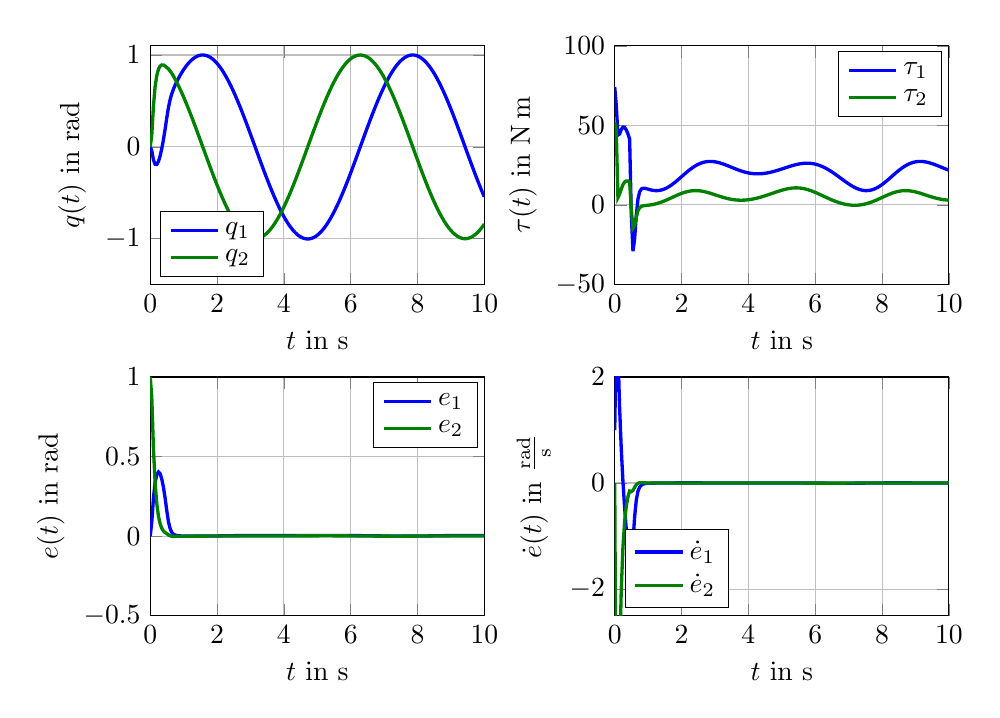
\begin{tikzpicture}

\begin{axis}[%
width=0.35\textwidth,
height=0.25\textwidth,
scale only axis,
xmin=0,
xmax=10,
xlabel={$t$ in $\mathrm{s}$},
xmajorgrids,
ymin=-1.5,
ymax=1.1,
ylabel={$q(t)$ in $\mathrm{rad}$},
ymajorgrids,
name=plot1,
legend style={at={(0.03,0.03)},anchor=south west,draw=black,fill=white,legend cell align=left}
]
\addplot [
color=blue,
solid,
line width=1.2pt
]
table[row sep=crcr]{
0 0\\
0.0462565125872653 -0.0415517317397441\\
0.0962565125872653 -0.143456795269038\\
0.146256512587265 -0.190667977776989\\
0.196256512587265 -0.192000503617512\\
0.246256512587265 -0.15933428766155\\
0.296256512587265 -0.0999239611473493\\
0.346256512587265 -0.0187974596933407\\
0.396256512587266 0.0802075683883657\\
0.446256512587266 0.193986969333029\\
0.496256512587266 0.318684541501134\\
0.546256512587266 0.430321839466557\\
0.596256512587266 0.515453901822797\\
0.646256512587266 0.579102231976597\\
0.696256512587266 0.629499564788814\\
0.746256512587266 0.672587311347751\\
0.796256512587266 0.711257265236233\\
0.846256512587266 0.746805575981871\\
0.896256512587266 0.779810396410792\\
0.946256512587266 0.810518119590678\\
0.996256512587266 0.839016897987885\\
1.04625651258726 0.865318852481635\\
1.09625651258726 0.88940047774863\\
1.14625651258725 0.911222935746489\\
1.19625651258724 0.930742389932213\\
1.24625651258724 0.947915329602158\\
1.29625651258723 0.962701350391994\\
1.34625651258723 0.975064633206133\\
1.39625651258722 0.984974750745877\\
1.44625651258722 0.992407121134606\\
1.49625651258721 0.997343271115281\\
1.54625651258721 0.99977099153365\\
1.5962565125872 0.999684427282644\\
1.64625651258719 0.997084123293553\\
1.69625651258719 0.991977037728256\\
1.74625651258718 0.984376528274685\\
1.79625651258718 0.974302314837438\\
1.84625651258717 0.961780420649887\\
1.89625651258717 0.946843093247658\\
1.94625651258716 0.929528706492668\\
1.99625651258716 0.909881644744986\\
2.04625651258715 0.887952170255581\\
2.09625651258715 0.863796274851346\\
2.14625651258714 0.837475516983224\\
2.19625651258713 0.80905684519989\\
2.24625651258713 0.778612409090586\\
2.29625651258712 0.746219358711058\\
2.34625651258712 0.711959633466678\\
2.39625651258711 0.675919741377157\\
2.44625651258711 0.638190529588206\\
2.4962565125871 0.598866946927741\\
2.5462565125871 0.558047799229027\\
2.59625651258709 0.515835498063035\\
2.64625651258708 0.472335803440724\\
2.69625651258708 0.427657560967747\\
2.74625651258707 0.381912433864235\\
2.79625651258707 0.335214630206151\\
2.84625651258706 0.287680625706404\\
2.89625651258706 0.239428882336488\\
2.94625651258705 0.190579563093821\\
2.99625651258705 0.141254243245243\\
3.04625651258704 0.0915756184203332\\
3.09625651258704 0.0416672099848423\\
3.14625651258703 -0.00834693181085684\\
3.19625651258702 -0.0583425263467672\\
3.24625651258702 -0.108195362187072\\
3.29625651258701 -0.157781596993471\\
3.34625651258701 -0.206978057076322\\
3.396256512587 -0.255662535833932\\
3.446256512587 -0.303714090317918\\
3.49625651258699 -0.351013335165121\\
3.54625651258699 -0.397442733152588\\
3.59625651258698 -0.442886881658985\\
3.64625651258697 -0.487232794350411\\
3.69625651258697 -0.530370177447309\\
3.74625651258696 -0.57219169996854\\
3.79625651258696 -0.612593257385334\\
3.84625651258695 -0.651474228148737\\
3.89625651258695 -0.688737722577154\\
3.94625651258694 -0.724290823603923\\
3.99625651258694 -0.758044818887772\\
4.04625651258695 -0.789915423781654\\
4.09625651258697 -0.819822994638631\\
4.14625651258698 -0.847692731908925\\
4.196256512587 -0.873454872452518\\
4.24625651258702 -0.897044870459616\\
4.29625651258703 -0.918403566340698\\
4.34625651258705 -0.937477342922383\\
4.39625651258707 -0.954218268269029\\
4.44625651258708 -0.968584224446649\\
4.4962565125871 -0.980539021558719\\
4.54625651258712 -0.990052496415599\\
4.59625651258713 -0.99710059525234\\
4.64625651258715 -1.00166543998412\\
4.69625651258717 -1.00373537758364\\
4.74625651258719 -1.00330501227813\\
4.7962565125872 -1.00037522039097\\
4.84625651258722 -0.994953147789569\\
4.89625651258724 -0.987052190039758\\
4.94625651258725 -0.976691955501697\\
4.99625651258727 -0.963898211724964\\
5.04625651258729 -0.948702815605823\\
5.0962565125873 -0.93114362785176\\
5.14625651258732 -0.911264412354314\\
5.19625651258734 -0.889114721099792\\
5.24625651258735 -0.864749765249684\\
5.29625651258737 -0.838230273001854\\
5.34625651258739 -0.809622334805012\\
5.3962565125874 -0.778997236448867\\
5.44625651258742 -0.74643128049786\\
5.49625651258744 -0.712005596484207\\
5.54625651258745 -0.675805940232436\\
5.59625651258747 -0.637922482657325\\
5.64625651258749 -0.598449588363364\\
5.6962565125875 -0.557485584377857\\
5.74625651258752 -0.515132519370974\\
5.79625651258754 -0.471495913752542\\
5.84625651258755 -0.426684501083749\\
5.89625651258757 -0.380809961298338\\
5.94625651258759 -0.333986646287948\\
5.9962565125876 -0.286331298465986\\
6.04625651258762 -0.237962762980063\\
6.09625651258764 -0.189001694291879\\
6.14625651258765 -0.139570257883434\\
6.19625651258767 -0.0897918278786146\\
6.24625651258769 -0.0397906813892845\\
6.2962565125877 0.0103083095944852\\
6.34625651258772 0.0603799879485591\\
6.39625651258774 0.11029922197732\\
6.44625651258775 0.15994121599041\\
6.49625651258777 0.209181820105879\\
6.54625651258779 0.257897838512306\\
6.5962565125878 0.305967335445761\\
6.64625651258782 0.353269938163107\\
6.69625651258784 0.399687136220675\\
6.74625651258785 0.445102576396328\\
6.79625651258787 0.489402352622967\\
6.84625651258789 0.532475290332056\\
6.8962565125879 0.574213224635809\\
6.94625651258792 0.614511271805351\\
6.99625651258794 0.653268093527764\\
7.04625651258795 0.690386153445919\\
7.09625651258797 0.725771965499268\\
7.14625651258799 0.75933633358937\\
7.196256512588 0.790994582089009\\
7.24625651258802 0.820666776696771\\
7.29625651258804 0.848277935109183\\
7.34625651258805 0.873758226940104\\
7.39625651258807 0.897043162263567\\
7.44625651258809 0.918073768094673\\
7.4962565125881 0.936796752057967\\
7.54625651258812 0.953164652430273\\
7.59625651258814 0.96713597369235\\
7.64625651258815 0.978675306689188\\
7.69625651258817 0.987753432489998\\
7.74625651258819 0.994347409063006\\
7.7962565125882 0.998440639941717\\
7.84625651258822 1.00002292416034\\
7.89625651258824 0.999090486875057\\
7.94625651258825 0.99564599025941\\
7.99625651258827 0.989698524457847\\
8.04625651258825 0.981263578590535\\
8.09625651258822 0.970362992012754\\
8.14625651258819 0.957024886231839\\
8.19625651258816 0.941283578063848\\
8.24625651258813 0.923179474763343\\
8.29625651258811 0.902758951979156\\
8.34625651258808 0.880074215475768\\
8.39625651258805 0.855183147616104\\
8.44625651258802 0.828149139630579\\
8.496256512588 0.799040910703726\\
8.54625651258797 0.767932314897781\\
8.59625651258794 0.734902136905722\\
8.64625651258791 0.700033877586688\\
8.69625651258789 0.66341553018606\\
8.74625651258786 0.625139348081722\\
8.79625651258783 0.585301604828317\\
8.8462565125878 0.544002347194653\\
8.89625651258777 0.501345141808581\\
8.94625651258775 0.457436815942901\\
8.99625651258772 0.412387192899908\\
9.04625651258769 0.366308822386526\\
9.09625651258766 0.319316706221375\\
9.14625651258764 0.271528019683661\\
9.19625651258761 0.223061828803689\\
9.24625651258758 0.174038803906427\\
9.29625651258755 0.124580929751311\\
9.34625651258752 0.0748112126597487\\
9.3962565125875 0.0248533850817381\\
9.44625651258747 -0.0251683918810231\\
9.49625651258744 -0.0751298274121235\\
9.54625651258741 -0.124906800733351\\
9.59625651258739 -0.174375660978476\\
9.64625651258736 -0.223413526455083\\
9.69625651258733 -0.271898582538894\\
9.7462565125873 -0.319710377437737\\
9.79625651258728 -0.366730115069655\\
9.84625651258725 -0.412840944319626\\
9.89625651258722 -0.457928243969216\\
9.94625651258719 -0.501879902629862\\
9.99625651258716 -0.544586593049829\\
};
\addlegendentry{$q_1$};

\addplot [
color=green!50!black,
solid,
line width=1.2pt
]
table[row sep=crcr]{
0 0\\
0.0462565125872653 0.12653042584566\\
0.0962565125872653 0.445993152378318\\
0.146256512587265 0.655648302770632\\
0.196256512587265 0.777509395996318\\
0.246256512587265 0.845184974099057\\
0.296256512587265 0.879139506144399\\
0.346256512587265 0.891775537937448\\
0.396256512587266 0.890590757493657\\
0.446256512587266 0.880121723745613\\
0.496256512587266 0.863969590674991\\
0.546256512587266 0.847238371859075\\
0.596256512587266 0.825721687132324\\
0.646256512587266 0.799296044636186\\
0.696256512587266 0.768942924086461\\
0.746256512587266 0.735882933112658\\
0.796256512587266 0.70078469301547\\
0.846256512587266 0.663938539244123\\
0.896256512587266 0.625489517745387\\
0.946256512587266 0.585535821132393\\
0.996256512587266 0.544164952773345\\
1.04625651258726 0.501466325274661\\
1.09625651258726 0.45753498685133\\
1.14625651258725 0.412472071478443\\
1.19625651258724 0.366384157042257\\
1.24625651258724 0.31938237125641\\
1.29625651258723 0.271581540871957\\
1.34625651258723 0.223099462888964\\
1.39625651258722 0.174056296519741\\
1.44625651258722 0.124574050897469\\
1.49625651258721 0.0747761413335615\\
1.54625651258721 0.0247869917194095\\
1.5962565125872 -0.0252683333369327\\
1.64625651258719 -0.0752644778458106\\
1.69625651258719 -0.125076132492481\\
1.74625651258718 -0.174578365847893\\
1.79625651258718 -0.223646951234509\\
1.84625651258717 -0.272158690450435\\
1.89625651258717 -0.319991734693322\\
1.94625651258716 -0.36702590245608\\
1.99625651258716 -0.413142993791753\\
2.04625651258715 -0.458227100100868\\
2.09625651258715 -0.502164908440223\\
2.14625651258714 -0.544845999261847\\
2.19625651258713 -0.586163136448723\\
2.24625651258713 -0.626012548510009\\
2.29625651258712 -0.664294199826588\\
2.34625651258712 -0.700912050893174\\
2.39625651258711 -0.735774306582284\\
2.44625651258711 -0.768793651554216\\
2.4962565125871 -0.799887472051674\\
2.5462565125871 -0.828978063442911\\
2.59625651258709 -0.855992823008035\\
2.64625651258708 -0.880864427593659\\
2.69625651258708 -0.903530995885904\\
2.74625651258707 -0.923936235165702\\
2.79625651258707 -0.942029572509268\\
2.84625651258706 -0.957766270477462\\
2.89625651258706 -0.971107527399029\\
2.94625651258705 -0.982020562394173\\
2.99625651258705 -0.99047868530794\\
3.04625651258704 -0.996461351729678\\
3.09625651258704 -0.999954203268701\\
3.14625651258703 -1.00094909324078\\
3.19625651258702 -0.999444097899048\\
3.24625651258702 -0.995443513320096\\
3.29625651258701 -0.988957838034388\\
3.34625651258701 -0.980003741472953\\
3.396256512587 -0.968604018290953\\
3.446256512587 -0.954787528625171\\
3.49625651258699 -0.938589124347028\\
3.54625651258699 -0.920049561385717\\
3.59625651258698 -0.899215398216761\\
3.64625651258697 -0.876138880639092\\
3.69625651258697 -0.8508778129972\\
3.74625651258696 -0.823495416042671\\
3.79625651258696 -0.794060171670086\\
3.84625651258695 -0.762645654804245\\
3.89625651258695 -0.729330352757737\\
3.94625651258694 -0.694197472418983\\
3.99625651258694 -0.657334735670128\\
4.04625651258695 -0.618834163471162\\
4.09625651258697 -0.578791849081239\\
4.14625651258698 -0.537307720920554\\
4.196256512587 -0.494485295606706\\
4.24625651258702 -0.450431421729065\\
4.29625651258703 -0.405256014953836\\
4.34625651258705 -0.359071785082282\\
4.39625651258707 -0.311993955715464\\
4.44625651258708 -0.264139977211492\\
4.4962565125871 -0.215629233655726\\
4.54625651258712 -0.166582744600381\\
4.59625651258713 -0.117122862366887\\
4.64625651258715 -0.067372965740849\\
4.69625651258717 -0.0174571509239174\\
4.74625651258719 0.0325000793627835\\
4.7962565125872 0.0823741277051001\\
4.84625651258722 0.132040613818479\\
4.89625651258724 0.181375685428964\\
4.94625651258725 0.230256327283419\\
4.99625651258727 0.27856066738244\\
5.04625651258729 0.326168279566195\\
5.0962565125873 0.372960481633693\\
5.14625651258732 0.418820628237675\\
5.19625651258734 0.463634397867737\\
5.24625651258735 0.507290073309276\\
5.29625651258737 0.549678815041142\\
5.34625651258739 0.590694927105457\\
5.3962565125874 0.630236115044364\\
5.44625651258742 0.668203735546416\\
5.49625651258744 0.704503037476794\\
5.54625651258745 0.739043393978865\\
5.59625651258747 0.771738525329597\\
5.64625651258749 0.802506712209401\\
5.6962565125875 0.831270999011062\\
5.74625651258752 0.857959386766582\\
5.79625651258754 0.882505015220039\\
5.84625651258755 0.904846333524171\\
5.89625651258757 0.92492725899369\\
5.94625651258759 0.942697323313856\\
5.9962565125876 0.958111805582499\\
6.04625651258762 0.971131851560094\\
6.09625651258764 0.981724578517113\\
6.14625651258765 0.989863165100905\\
6.19625651258767 0.995526925694905\\
6.24625651258769 0.998701368809205\\
6.2962565125877 0.999378239120927\\
6.34625651258772 0.997555542872394\\
6.39625651258774 0.993237556431688\\
6.44625651258775 0.986434817920511\\
6.49625651258777 0.977164101915287\\
6.54625651258779 0.965448377326444\\
6.5962565125878 0.951316748655186\\
6.64625651258782 0.934804380915045\\
6.69625651258784 0.915952408585204\\
6.74625651258785 0.894807829033123\\
6.79625651258787 0.8714233809043\\
6.84625651258789 0.845857408026928\\
6.8962565125879 0.818173709418314\\
6.94625651258792 0.788441376008634\\
6.99625651258794 0.756734614715995\\
7.04625651258795 0.723132560515568\\
7.09625651258797 0.687719077145273\\
7.14625651258799 0.650582547082021\\
7.196256512588 0.611815651406812\\
7.24625651258802 0.571515140155057\\
7.29625651258804 0.529781593721711\\
7.34625651258805 0.486719175860474\\
7.39625651258807 0.442435378784177\\
7.44625651258809 0.39704076084127\\
7.4962565125881 0.350648677213041\\
7.54625651258812 0.303375004049992\\
7.59625651258814 0.255337856445886\\
7.64625651258815 0.206657300636472\\
7.69625651258817 0.157455060808862\\
7.74625651258819 0.107854220918647\\
7.7962565125882 0.0579789219362689\\
7.84625651258822 0.00795405498242596\\
7.89625651258824 -0.0420950491359368\\
7.94625651258825 -0.0920429334133873\\
7.99625651258827 -0.141764330507568\\
8.04625651258825 -0.191134480243001\\
8.09625651258822 -0.240029447940244\\
8.14625651258819 -0.288326442668259\\
8.19625651258816 -0.335904134436742\\
8.24625651258813 -0.382642969272157\\
8.29625651258811 -0.428425481059565\\
8.34625651258808 -0.473136598985299\\
8.39625651258805 -0.516663949385448\\
8.44625651258802 -0.558898150794057\\
8.496256512588 -0.599733100994143\\
8.54625651258797 -0.639066254905027\\
8.59625651258794 -0.67679889219113\\
8.64625651258791 -0.712836373549586\\
8.69625651258789 -0.74708838472536\\
8.74625651258786 -0.779469167410206\\
8.79625651258783 -0.809897736302398\\
8.8462565125878 -0.838298081733009\\
8.89625651258777 -0.864599357396519\\
8.94625651258775 -0.888736052853184\\
8.99625651258772 -0.910648150592553\\
9.04625651258769 -0.93028126755696\\
9.09625651258766 -0.94758678111704\\
9.14625651258764 -0.962521939565733\\
9.19625651258761 -0.975049957251811\\
9.24625651258758 -0.985140094509088\\
9.29625651258755 -0.992767722554698\\
9.34625651258752 -0.997914373531911\\
9.3962565125875 -1.00056777586324\\
9.44625651258747 -1.00072187506182\\
9.49625651258744 -0.998376840127004\\
9.54625651258741 -0.99353905562738\\
9.59625651258739 -0.986221099553959\\
9.64625651258736 -0.976441707010923\\
9.69625651258733 -0.96422571980244\\
9.7462565125873 -0.949604021973181\\
9.79625651258728 -0.932613461367607\\
9.84625651258725 -0.91329675728873\\
9.89625651258722 -0.891702394360295\\
9.94625651258719 -0.867884502726143\\
9.99625651258716 -0.841902724755606\\
};
\addlegendentry{$q_2$};

\end{axis}

\begin{axis}[%
width=0.35\textwidth,
height=0.25\textwidth,
scale only axis,
xmin=0,
xmax=10,
xlabel={$t$ in $\mathrm{s}$},
xmajorgrids,
ymin=-0.5,
ymax=1,
ylabel={$e(t)$ in $\mathrm{rad}$},
ymajorgrids,
name=plot3,
at=(plot1.below south west),
anchor=above north west,
legend style={draw=black,fill=white,legend cell align=left}
]
\addplot [
color=blue,
solid,
line width=1.2pt
]
table[row sep=crcr]{
0 0\\
0.0462565125872653 0.0877917505185021\\
0.0962565125872653 0.239564735530334\\
0.146256512587265 0.336403619722218\\
0.196256512587265 0.386999584039465\\
0.246256512587265 0.403109410412731\\
0.296256512587265 0.391865815376509\\
0.346256512587265 0.358176342805285\\
0.396256512587266 0.30576007314369\\
0.446256512587266 0.237604712523369\\
0.496256512587266 0.157452426243568\\
0.546256512587266 0.0891703197144275\\
0.596256512587266 0.0460949889428037\\
0.646256512587266 0.0230998105957143\\
0.696256512587266 0.0118504381045387\\
0.746256512587266 0.006307610868034\\
0.796256512587266 0.00348569255808651\\
0.846256512587266 0.0019989322274333\\
0.896256512587266 0.00118404091282232\\
0.946256512587266 0.000714167487978701\\
0.996256512587266 0.000425580609724752\\
1.04625651258726 0.000235648611623729\\
1.09625651258726 0.000102610359614896\\
1.14625651258725 5.44490072418302e-06\\
1.19625651258724 -6.6313139081009e-05\\
1.24625651258724 -0.000117762168358793\\
1.29625651258723 -0.000151292632680433\\
1.34625651258723 -0.000167958979323979\\
1.39625651258722 -0.000168194020764956\\
1.44625651258722 -0.000152185425662643\\
1.49625651258721 -0.000120077005397623\\
1.54625651258721 -7.20776643009513e-05\\
1.5962565125872 -8.52030537201731e-06\\
1.64625651258719 7.0107645347095e-05\\
1.69625651258719 0.00016315090281005\\
1.74625651258718 0.000269784273592144\\
1.79625651258718 0.000389018640567063\\
1.84625651258717 0.000519713033583891\\
1.89625651258717 0.000660591463293558\\
1.94625651258716 0.000810263484367191\\
1.99625651258716 0.000967247584359177\\
2.04625651258715 0.00112999655618506\\
2.09625651258715 0.00129692405085402\\
2.14625651258714 0.00146643154398374\\
2.19625651258713 0.00163693499352768\\
2.24625651258713 0.00180689051971794\\
2.29625651258712 0.00197481850162184\\
2.34625651258712 0.00213932555734098\\
2.39625651258711 0.00229912395619036\\
2.44625651258711 0.00245304810069336\\
2.4962565125871 0.00260006781321454\\
2.5462565125871 0.002739298265098\\
2.59625651258709 0.00287000649280045\\
2.64625651258708 0.00299161455203639\\
2.69625651258708 0.00310369946269057\\
2.74625651258707 0.00320599018893131\\
2.79625651258707 0.00329836197540972\\
2.84625651258706 0.00338082841725629\\
2.89625651258706 0.00345353167583765\\
2.94625651258705 0.00351673126285518\\
2.99625651258705 0.00357079180328759\\
3.04625651258704 0.00361617015585169\\
3.09625651258704 0.00365340222248131\\
3.14625651258703 0.00368308972131941\\
3.19625651258702 0.00370588713671056\\
3.24625651258702 0.00372248900030941\\
3.29625651258701 0.00373361760454913\\
3.34625651258701 0.00374001120707601\\
3.396256512587 0.0037424127547071\\
3.446256512587 0.00374155913894775\\
3.49625651258699 0.00373817099167906\\
3.54625651258699 0.00373294303769761\\
3.59625651258698 0.00372653503783854\\
3.64625651258697 0.00371956337927426\\
3.69625651258697 0.00371259339478558\\
3.74625651258696 0.0037061325167943\\
3.79625651258696 0.00370062439143459\\
3.84625651258695 0.00369644409001402\\
3.89625651258695 0.0036938945576066\\
3.94625651258694 0.0036932044296708\\
3.99625651258694 0.00369452732676367\\
4.04625651258695 0.00369794270474266\\
4.09625651258697 0.00370345829435981\\
4.14625651258698 0.00371101411131836\\
4.196256512587 0.00372048795888891\\
4.24625651258702 0.00373170228228792\\
4.29625651258703 0.00374443217161247\\
4.34625651258705 0.00375841425169465\\
4.39625651258707 0.00377335614699836\\
4.44625651258708 0.00378894617144154\\
4.4962565125871 0.0038048628703562\\
4.54625651258712 0.00382078403748687\\
4.59625651258713 0.00383639484587917\\
4.64625651258715 0.00385139476833085\\
4.69625651258717 0.00386550302005995\\
4.74625651258719 0.00387846233099953\\
4.7962565125872 0.00389004094387568\\
4.84625651258722 0.00390003283167517\\
4.89625651258724 0.00390825622798041\\
4.94625651258725 0.00391455065910451\\
4.99625651258727 0.00391877275098518\\
5.04625651258729 0.00392079115026756\\
5.0962565125873 0.00392048094280117\\
5.14625651258732 0.00391771797074547\\
5.19625651258734 0.00391237344055073\\
5.24625651258735 0.00390430917944851\\
5.29625651258737 0.00389337384115473\\
5.34625651258739 0.00387940028749423\\
5.3962565125874 0.00386220428801798\\
5.44625651258742 0.0038415845915617\\
5.49625651258744 0.00381732433898907\\
5.54625651258745 0.00378919371134012\\
5.59625651258747 0.00375695364709827\\
5.64625651258749 0.00372036041951107\\
5.6962565125875 0.00367917084124381\\
5.74625651258752 0.00363314785863789\\
5.79625651258754 0.00358206630954128\\
5.84625651258755 0.00352571864387197\\
5.89625651258757 0.00346392044085048\\
5.94625651258759 0.00339651559697551\\
5.9962565125876 0.00332338110024422\\
6.04625651258762 0.00324443134529312\\
6.09625651258764 0.00315962197822403\\
6.14625651258765 0.00306895328699811\\
6.19625651258767 0.00297247317238385\\
6.24625651258769 0.00287027974537878\\
6.2962565125877 0.00276252360027052\\
6.34625651258772 0.00264940980902937\\
6.39625651258774 0.00253119967378321\\
6.44625651258775 0.00240821226102747\\
6.49625651258777 0.00228082572521143\\
6.54625651258779 0.00214947841147634\\
6.5962565125878 0.0020146697084289\\
6.64625651258782 0.00187696060253151\\
6.69625651258784 0.00173697386642602\\
6.74625651258785 0.00159539379465334\\
6.79625651258787 0.00145296538222178\\
6.84625651258789 0.0013104928248352\\
6.8962565125879 0.00116883720515248\\
6.94625651258792 0.00102891321826282\\
6.99625651258794 0.000891684783073776\\
7.04625651258795 0.000758159386190838\\
7.09625651258797 0.000629381013033004\\
7.14625651258799 0.000506421539347768\\
7.196256512588 0.000390370486760272\\
7.24625651258802 0.00028232308992493\\
7.29625651258804 0.000183366680997166\\
7.34625651258805 9.45654691887343e-05\\
7.39625651258807 1.6943877549247e-05\\
7.44625651258809 -4.85313072146054e-05\\
7.4962565125881 -0.000100969617835789\\
7.54625651258812 -0.000139575971837225\\
7.59625651258814 -0.000163669580892978\\
7.64625651258815 -0.000172702095548427\\
7.69625651258817 -0.000166274331356076\\
7.74625651258819 -0.000144150909311414\\
7.7962565125882 -0.000106272167307409\\
7.84625651258822 -5.27627621642601e-05\\
7.89625651258824 1.60635177791635e-05\\
7.94625651258825 9.97030767366791e-05\\
7.99625651258827 0.000197466162600635\\
8.04625651258825 0.000308484865534364\\
8.09625651258822 0.000431725313148834\\
8.14625651258819 0.000566003750700372\\
8.19625651258816 0.000710006054070011\\
8.24625651258813 0.000862310110435804\\
8.29625651258811 0.00102141041996084\\
8.34625651258808 0.00118574422240569\\
8.39625651258805 0.00135371843319809\\
8.44625651258802 0.00152373668050676\\
8.496256512588 0.0016942257636503\\
8.54625651258797 0.00186366089951628\\
8.59625651258794 0.00203058918399956\\
8.64625651258791 0.00219365076738087\\
8.69625651258789 0.00235159732449941\\
8.74625651258786 0.00250330749137184\\
8.79625651258783 0.00264779903835566\\
8.8462565125878 0.00278423765406433\\
8.89625651258777 0.00291194232100844\\
8.94625651258775 0.00303038736925171\\
8.99625651258772 0.00313920139321178\\
9.04625651258769 0.00323816330379206\\
9.09625651258766 0.00332719585826735\\
9.14625651258764 0.00340635705980252\\
9.19625651258761 0.0034758298447935\\
9.24625651258758 0.00353591047898594\\
9.29625651258755 0.0035869960641922\\
9.34625651258752 0.00362957151987246\\
9.3962565125875 0.00366419635272279\\
9.44625651258747 0.00369149146840689\\
9.49625651258744 0.00371212621850821\\
9.54625651258741 0.00372680581810104\\
9.59625651258739 0.00373625921955742\\
9.64625651258736 0.00374122748961014\\
9.69625651258733 0.00374245271115803\\
9.7462565125873 0.00374066741929374\\
9.79625651258728 0.0037365845817055\\
9.84625651258725 0.00373088814501321\\
9.89625651258722 0.00372422418797735\\
9.94625651258719 0.00371719274656801\\
9.99625651258716 0.00371034040106255\\
};
\addlegendentry{$e_1$};

\addplot [
color=green!50!black,
solid,
line width=1.2pt
]
table[row sep=crcr]{
0 1\\
0.0462565125872653 0.872399932419289\\
0.0962565125872653 0.549377765329614\\
0.146256512587265 0.333675265465166\\
0.196256512587265 0.203294029076511\\
0.246256512587265 0.12464681004067\\
0.296256512587265 0.0772965626805072\\
0.346256512587265 0.04887422350285\\
0.396256512587266 0.0319215620393577\\
0.446256512587266 0.0219473535164147\\
0.496256512587266 0.0154015414113876\\
0.546256512587266 0.00723684518907219\\
0.596256512587266 0.00172187183706196\\
0.646256512587266 -0.000952321718709404\\
0.696256512587266 -0.0016944807588144\\
0.746256512587266 -0.00164749090789573\\
0.796256512587266 -0.00139745815667702\\
0.846256512587266 -0.00114761558461607\\
0.896256512587266 -0.000951537419473514\\
0.946256512587266 -0.000811803837795777\\
0.996256512587266 -0.000716404034919571\\
1.04625651258726 -0.000651583441715009\\
1.09625651258726 -0.00060582795917058\\
1.14625651258725 -0.000570580460193482\\
1.19625651258724 -0.000539873111313816\\
1.24625651258724 -0.000509714594579991\\
1.29625651258723 -0.000477527055225302\\
1.34625651258723 -0.000441710763631004\\
1.39625651258722 -0.000401334508204676\\
1.44625651258722 -0.000355925967001666\\
1.49625651258721 -0.000305334104940852\\
1.54625651258721 -0.000249640427060147\\
1.5962565125872 -0.0001891019064146\\
1.64625651258719 -0.000124113603100925\\
1.69625651258719 -5.51829449919605e-05\\
1.74625651258718 1.70895433225515e-05\\
1.79625651258718 9.2026343847279e-05\\
1.84625651258717 0.000168887860754807\\
1.89625651258717 0.000246887261546258\\
1.94625651258716 0.000325205780889959\\
1.99625651258716 0.000403008640806113\\
2.04625651258715 0.000479461486211474\\
2.09625651258715 0.000553747068031463\\
2.14625651258714 0.000625081801508554\\
2.19625651258713 0.000692731769112553\\
2.24625651258713 0.000756027715733687\\
2.29625651258712 0.000814378592331466\\
2.34625651258712 0.000867283238410232\\
2.39625651258711 0.000914339849881762\\
2.44625651258711 0.000955252953333763\\
2.4962565125871 0.000989837696305784\\
2.5462565125871 0.00101802136110007\\
2.59625651258709 0.00103984211173025\\
2.64625651258708 0.00105544508419597\\
2.69625651258708 0.00106507602389516\\
2.74625651258707 0.00106907275563739\\
2.79625651258707 0.0010678548372437\\
2.84625651258706 0.0010619117942684\\
2.89625651258706 0.00105179035937508\\
2.94625651258705 0.00103808114539583\\
2.99625651258705 0.00102140516736093\\
3.04625651258704 0.00100240059825774\\
3.09625651258704 0.000981710099267397\\
3.14625651258703 0.000959969011436024\\
3.19625651258702 0.000937794636104439\\
3.24625651258702 0.000915776769675691\\
3.29625651258701 0.000894469597833791\\
3.34625651258701 0.000874384997900046\\
3.396256512587 0.000855987247878498\\
3.446256512587 0.00083968909824883\\
3.49625651258699 0.000825849128644918\\
3.54625651258699 0.000814770286245436\\
3.59625651258698 0.000806699485723983\\
3.64625651258697 0.000801828141112071\\
3.69625651258697 0.000800293496796445\\
3.74625651258696 0.000802180626779614\\
3.79625651258696 0.000807524976892404\\
3.84625651258695 0.000816315332489603\\
3.89625651258695 0.000828497103047998\\
3.94625651258694 0.00084397582406448\\
3.99625651258694 0.000862620784947254\\
4.04625651258695 0.000884268698878254\\
4.09625651258697 0.000908727336701665\\
4.14625651258698 0.000935779052412822\\
4.196256512587 0.000965184132525276\\
4.24625651258702 0.000996683907225127\\
4.29625651258703 0.00103000356780608\\
4.34625651258705 0.00106485464369072\\
4.39625651258707 0.00110093710400277\\
4.44625651258708 0.00113794106373605\\
4.4962565125871 0.00117554809323236\\
4.54625651258712 0.00121343215173608\\
4.59625651258713 0.0012512601905397\\
4.64625651258715 0.00128869249747647\\
4.69625651258717 0.00132538288060384\\
4.74625651258719 0.0013609788128079\\
4.7962565125872 0.00139512167845528\\
4.84625651258722 0.00142744727576327\\
4.89625651258724 0.00145758673205196\\
4.94625651258725 0.00148516798169437\\
4.99625651258727 0.00150981793724669\\
5.04625651258729 0.00153116545265319\\
5.0962565125873 0.001548845134342\\
5.14625651258732 0.00156250200331193\\
5.19625651258734 0.00157179695190135\\
5.24625651258735 0.00157641287666699\\
5.29625651258737 0.00157606130818233\\
5.34625651258739 0.00157048930436443\\
5.3962565125874 0.0015594863307955\\
5.44625651258742 0.00154289082343073\\
5.49625651258744 0.00152059611911515\\
5.54625651258745 0.00149255544911553\\
5.59625651258747 0.00145878572055091\\
5.64625651258749 0.0014193698586632\\
5.6962565125875 0.00137445754635768\\
5.74625651258752 0.00132426427216881\\
5.79625651258754 0.00126906867871912\\
5.84625651258755 0.00120920828549154\\
5.89625651258757 0.00114507373695538\\
5.94625651258759 0.00107710179509179\\
5.9962565125876 0.00100576735019697\\
6.04625651258762 0.000931574762792819\\
6.09625651258764 0.000855048871001851\\
6.14625651258765 0.000776726001543437\\
6.19625651258767 0.000697145309401903\\
6.24625651258769 0.000616840742913793\\
6.2962565125877 0.000536333889984975\\
6.34625651258772 0.000456127910225756\\
6.39625651258774 0.000376702700110809\\
6.44625651258775 0.000298511376940147\\
6.49625651258777 0.000221978105353737\\
6.54625651258779 0.000147497230164828\\
6.5962565125878 7.54336236069575e-05\\
6.64625651258782 6.12410570532962e-06\\
6.69625651258784 -6.01202451514515e-05\\
6.74625651258785 -0.000123011107135307\\
6.79625651258787 -0.000182279494348792\\
6.84625651258789 -0.000237672152945012\\
6.8962565125879 -0.000288948029740665\\
6.94625651258792 -0.00033587506279309\\
6.99625651258794 -0.000378227527841335\\
7.04625651258795 -0.000415784150282539\\
7.09625651258797 -0.000448327160148532\\
7.14625651258799 -0.000475642428333867\\
7.196256512588 -0.000497520777065663\\
7.24625651258802 -0.000513760507499628\\
7.29625651258804 -0.000524171133693185\\
7.34625651258805 -0.000528578256528189\\
7.39625651258807 -0.00052682945514565\\
7.44625651258809 -0.00051880101895363\\
7.4962565125881 -0.000504405292350518\\
7.54625651258812 -0.000483598359117821\\
7.59625651258814 -0.000456387756261445\\
7.64625651258815 -0.000422839880119125\\
7.69625651258817 -0.000383086732840709\\
7.74625651258819 -0.00033733165664461\\
7.7962565125882 -0.000285853717727706\\
7.84625651258822 -0.000229010431922953\\
7.89625651258824 -0.000167238569849217\\
7.94625651258825 -0.000101052839197174\\
7.99625651258827 -3.10423138436544e-05\\
8.04625651258825 4.2135439253993e-05\\
8.09625651258822 0.000117762497204299\\
8.14625651258819 0.000195070855942947\\
8.19625651258816 0.000273254628761821\\
8.24625651258813 0.000351483874847847\\
8.29625651258811 0.00042891969286335\\
8.34625651258808 0.000504730156319133\\
8.39625651258805 0.000578106624342434\\
8.44625651258802 0.000648279935415719\\
8.496256512588 0.000714535984198239\\
8.54625651258797 0.000776230193465066\\
8.59625651258794 0.000832800424707791\\
8.64625651258791 0.000883777921383166\\
8.69625651258789 0.000928795946701033\\
8.74625651258786 0.000967595860632664\\
8.79625651258783 0.00100003047500186\\
8.8462565125878 0.00102606462657506\\
8.89625651258777 0.00104577301097297\\
8.94625651258775 0.00105933541947478\\
8.99625651258772 0.00106702961116445\\
9.04625651258769 0.00106922212965255\\
9.09625651258766 0.00106635743310191\\
9.14625651258764 0.00105894574606302\\
9.19625651258761 0.00104755006070734\\
9.24625651258758 0.00103277271387869\\
9.29625651258755 0.00101524194668279\\
9.34625651258752 0.000995598817899568\\
9.3962565125875 0.000974484794751596\\
9.44625651258747 0.000952530288400033\\
9.49625651258744 0.000930344340778766\\
9.54625651258741 0.000908505607716492\\
9.59625651258739 0.000887554723905892\\
9.64625651258736 0.000867988080762716\\
9.69625651258733 0.000850253000523993\\
9.7462565125873 0.00083474425026675\\
9.79625651258728 0.000821801808510991\\
9.84625651258725 0.000811709774632075\\
9.89625651258722 0.000804696296951457\\
9.94625651258719 0.000800934388158536\\
9.99625651258716 0.000800543495429351\\
};
\addlegendentry{$e_2$};

\end{axis}

\begin{axis}[%
width=0.35\textwidth,
height=0.25\textwidth,
scale only axis,
xmin=0,
xmax=10,
xlabel={$t$ in $\mathrm{s}$},
xmajorgrids,
ymin=-2.5,
ymax=2,
ylabel={$\dot{e}(t)$ in $\mathrm{\frac{rad}{s}}$},
ymajorgrids,
name=plot2,
at=(plot3.right of south east),
anchor=left of south west,
legend style={at={(0.03,0.03)},anchor=south west,draw=black,fill=white,legend cell align=left}
]
\addplot [
color=blue,
solid,
line width=1.2pt
]
table[row sep=crcr]{
0 1\\
0.0462565125872653 2.78260202554259\\
0.0962565125872653 2.51912716145275\\
0.146256512587265 1.42350673667473\\
0.196256512587265 0.637859217875422\\
0.246256512587265 0.0295835400375724\\
0.296256512587265 -0.463280523238772\\
0.346256512587265 -0.872039355557777\\
0.396256512587266 -1.21471960066204\\
0.446256512587266 -1.50326769482586\\
0.496256512587266 -1.60062664893443\\
0.546256512587266 -1.10788864160594\\
0.596256512587266 -0.634049969577842\\
0.646256512587266 -0.316057405158356\\
0.696256512587266 -0.153903020758199\\
0.746256512587266 -0.0771884249565129\\
0.796256512587266 -0.0400380154922186\\
0.846256512587266 -0.0215273735571229\\
0.896256512587266 -0.0121050034779415\\
0.946256512587266 -0.00721042870561317\\
0.996256512587266 -0.00459600171280894\\
1.04625651258726 -0.00313421244239631\\
1.09625651258726 -0.00225420926296949\\
1.14625651258725 -0.00166567237581922\\
1.19625651258724 -0.00122081185314843\\
1.24625651258724 -0.000844687081365592\\
1.29625651258723 -0.000499821042238113\\
1.34625651258723 -0.000168155449665613\\
1.39625651258722 0.000158193994042377\\
1.44625651258722 0.000481707811280707\\
1.49625651258721 0.000801954849399253\\
1.54625651258721 0.00111692287321996\\
1.5962565125872 0.00142375546388335\\
1.64625651258719 0.00171918372607881\\
1.69625651258719 0.00199979896785024\\
1.74625651258718 0.00226223991317229\\
1.79625651258718 0.00250333099167979\\
1.84625651258717 0.00272018946222879\\
1.89625651258717 0.00291030971851292\\
1.94625651258716 0.0030716285586202\\
1.99625651258716 0.00320257312855704\\
2.04625651258715 0.00330209244288715\\
2.09625651258715 0.00336967319340342\\
2.14625651258714 0.00340534063753595\\
2.19625651258713 0.00340964553786405\\
2.24625651258713 0.00338363832385236\\
2.29625651258712 0.00332883183811483\\
2.34625651258712 0.00324715420806621\\
2.39625651258711 0.00314089355271019\\
2.44625651258711 0.00301263639276783\\
2.4962565125871 0.00286520177075111\\
2.5462565125871 0.00270157318796327\\
2.59625651258709 0.00252483050410157\\
2.64625651258708 0.0023380838991115\\
2.69625651258708 0.00214441184935865\\
2.74625651258707 0.00194680481585208\\
2.79625651258707 0.00174811598985625\\
2.84625651258706 0.00155102001365037\\
2.89625651258706 0.00135798012527932\\
2.94625651258705 0.0011712237060939\\
2.99625651258705 0.000992725779450976\\
3.04625651258704 0.000824199653537527\\
3.09625651258704 0.000667093647285455\\
3.14625651258703 0.000522592699696234\\
3.19625651258702 0.000391623640978889\\
3.24625651258702 0.000274862988529967\\
3.29625651258701 0.000172746302437354\\
3.34625651258701 8.54783681212279e-05\\
3.396256512587 1.30437397112271e-05\\
3.446256512587 -4.47825518425926e-05\\
3.49625651258699 -8.84240723495466e-05\\
3.54625651258699 -0.000118491578801283\\
3.59625651258698 -0.000135770724291606\\
3.64625651258697 -0.000141208380860958\\
3.69625651258697 -0.00013589707675854\\
3.74625651258696 -0.000121057102812738\\
3.79625651258696 -9.80159635910471e-05\\
3.84625651258695 -6.81850222316038e-05\\
3.89625651258695 -3.30333997232701e-05\\
3.94625651258694 5.94057575997731e-06\\
3.99625651258694 4.72398326679668e-05\\
4.04625651258695 8.94001662957722e-05\\
4.09625651258697 0.000131022025633643\\
4.14625651258698 0.000170801349534511\\
4.196256512587 0.00020755822065871\\
4.24625651258702 0.000240262073165576\\
4.29625651258703 0.000268052231669647\\
4.34625651258705 0.000290252681578229\\
4.39625651258707 0.000306380173409615\\
4.44625651258708 0.000316145041257931\\
4.4962565125871 0.000319444457316798\\
4.54625651258712 0.00031634823405946\\
4.59625651258713 0.000307077701449485\\
4.64625651258715 0.000291978601941023\\
4.69625651258717 0.000271489330918633\\
4.74625651258719 0.00024610617335618\\
4.7962565125872 0.000216347418933199\\
4.84625651258722 0.000182718352219807\\
4.89625651258724 0.000145679095133772\\
4.94625651258725 0.00010561711888038\\
4.99625651258727 6.28259491283756e-05\\
5.04625651258729 1.74911801507638e-05\\
5.0962565125873 -3.03155776408826e-05\\
5.14625651258732 -8.06347271171126e-05\\
5.19625651258734 -0.000133609134329804\\
5.24625651258735 -0.000189467928957354\\
5.29625651258737 -0.000248504984251996\\
5.34625651258739 -0.00031105368570572\\
5.3962565125874 -0.000377459739717256\\
5.44625651258742 -0.0004480537728766\\
5.49625651258744 -0.000523125337766106\\
5.54625651258745 -0.000602899694411518\\
5.59625651258747 -0.00068751840771053\\
5.64625651258749 -0.000777024426749207\\
5.6962565125875 -0.000871351928445674\\
5.74625651258752 -0.000970320849730366\\
5.79625651258754 -0.00107363572724051\\
5.84625651258755 -0.00118088823096429\\
5.89625651258757 -0.00129156262863772\\
5.94625651258759 -0.00140504335235392\\
5.9962565125876 -0.00152062385058327\\
6.04625651258762 -0.00163751598508244\\
6.09625651258764 -0.00175485935575637\\
6.14625651258765 -0.00187173008937847\\
6.19625651258767 -0.00198714879240347\\
6.24625651258769 -0.00210008752868496\\
6.2962565125877 -0.00220947582819409\\
6.34625651258772 -0.00231420585526487\\
6.39625651258774 -0.00241313696111867\\
6.44625651258775 -0.00250509991565229\\
6.49625651258777 -0.00258890116041521\\
6.54625651258779 -0.00266332745272868\\
6.5962565125878 -0.00272715128460876\\
6.64625651258782 -0.00277913746349423\\
6.69625651258784 -0.00281805123717027\\
6.74625651258785 -0.00284266833312319\\
6.79625651258787 -0.00285178726101465\\
6.84625651258789 -0.00284424419220086\\
6.8962565125879 -0.0028189306767189\\
6.94625651258792 -0.00277481437972271\\
6.99625651258794 -0.00271096290949191\\
7.04625651258795 -0.00262657066310512\\
7.09625651258797 -0.00252098843032167\\
7.14625651258799 -0.002393755272455\\
7.196256512588 -0.00224463193584645\\
7.24625651258802 -0.00207363478006595\\
7.29625651258804 -0.00188106891612017\\
7.34625651258805 -0.00166755898274551\\
7.39625651258807 -0.00143407576745486\\
7.44625651258809 -0.00118195673519145\\
7.4962565125881 -0.000912918493071513\\
7.54625651258812 -0.000629059322969694\\
7.59625651258814 -0.000332850174519839\\
7.64625651258815 -2.71129356785305e-05\\
7.69625651258817 0.000285014624575503\\
7.74625651258819 0.000600127147465657\\
7.7962565125882 0.000914612344275728\\
7.84625651258822 0.0012247223810303\\
7.89625651258824 0.00152665363238039\\
7.94625651258825 0.00181663187456362\\
7.99625651258827 0.0020909996094079\\
8.04625651258825 0.00234630206625183\\
8.09625651258822 0.00257936852429094\\
8.14625651258819 0.00278738591440991\\
8.19625651258816 0.00296796214673384\\
8.24625651258813 0.00311917721318394\\
8.29625651258811 0.00323962075792195\\
8.34625651258808 0.00332841543817786\\
8.39625651258805 0.00338522596617918\\
8.44625651258802 0.00341025420503394\\
8.496256512588 0.00340422108301452\\
8.54625651258797 0.00336833640269174\\
8.59625651258794 0.00330425787384758\\
8.64625651258791 0.003214040912633\\
8.69625651258789 0.003100080937813\\
8.74625651258786 0.00296505006168335\\
8.79625651258783 0.00281183020928266\\
8.8462565125878 0.00264344478666734\\
8.89625651258777 0.00246299103456338\\
8.94625651258775 0.00227357512658466\\
8.99625651258772 0.00207825188875255\\
9.04625651258769 0.00187997072865109\\
9.09625651258766 0.00168152898205221\\
9.14625651258764 0.00148553343943147\\
9.19625651258761 0.00129437034097801\\
9.24625651258758 0.00111018366768445\\
9.29625651258755 0.000934861147353194\\
9.34625651258752 0.000770027070779666\\
9.3962565125875 0.000617040797190493\\
9.44625651258747 0.000476999729144389\\
9.49625651258744 0.000350745552661902\\
9.54625651258741 0.000238872654793831\\
9.59625651258739 0.000141737826193755\\
9.64625651258736 5.94706035051962e-05\\
9.69625651258733 -8.01612306189359e-06\\
9.7462565125873 -6.10153455281592e-05\\
9.79625651258728 -0.000100014888449573\\
9.84625651258725 -0.000125685755547722\\
9.89625651258722 -0.000138869426823396\\
9.94625651258719 -0.000140563601991328\\
9.99625651258716 -0.00013190589876888\\
};
\addlegendentry{$\dot{e}_1$};

\addplot [
color=green!50!black,
solid,
line width=1.2pt
]
table[row sep=crcr]{
0 -0\\
0.0462565125872653 -5.44803309666348\\
0.0962565125872653 -5.48690146053898\\
0.146256512587265 -3.32011070223134\\
0.196256512587265 -2.00445371769418\\
0.246256512587265 -1.20791817860963\\
0.296256512587265 -0.726301791668329\\
0.346256512587265 -0.434825546273471\\
0.396256512587266 -0.257870488733374\\
0.446256512587266 -0.149907078190573\\
0.496256512587266 -0.161112348181745\\
0.546256512587266 -0.140964870361001\\
0.596256512587266 -0.0803579442892499\\
0.646256512587266 -0.0298029561107795\\
0.696256512587266 -0.00401762258424254\\
0.746256512587266 0.00407144243127799\\
0.796256512587266 0.00532801181079412\\
0.846256512587266 0.00451595189449361\\
0.896256512587266 0.00332910943307174\\
0.946256512587266 0.0023039587195669\\
0.996256512587266 0.0015589813980964\\
1.04625651258726 0.00107237165688934\\
1.09625651258726 0.000786214379604022\\
1.14625651258725 0.000643361850455659\\
1.19625651258724 0.000598044896593097\\
1.24625651258724 0.000616741979734159\\
1.29625651258723 0.000675987143782253\\
1.34625651258723 0.000759695792012516\\
1.39625651258722 0.000856878451427234\\
1.44625651258722 0.00095993081610668\\
1.49625651258721 0.00106344502133393\\
1.54625651258721 0.00116342359041566\\
1.5962565125872 0.00125678105268634\\
1.64625651258719 0.00134104153588688\\
1.69625651258719 0.00141416539564965\\
1.74625651258718 0.00147445829084392\\
1.79625651258718 0.00152053112963624\\
1.84625651258717 0.00155128977972474\\
1.89625651258717 0.00156594050493419\\
1.94625651258716 0.00156400179138105\\
1.99625651258716 0.0015453163500867\\
2.04625651258715 0.00151005918764435\\
2.09625651258715 0.00145873909756278\\
2.14625651258714 0.00139219198563867\\
2.19625651258713 0.00131156525615272\\
2.24625651258713 0.00121829314411059\\
2.29625651258712 0.00111406343366005\\
2.34625651258712 0.00100077647882868\\
2.39625651258711 0.000880497846053152\\
2.44625651258711 0.000755406223538757\\
2.4962565125871 0.000627738479301532\\
2.5462565125871 0.000499733886257459\\
2.59625651258709 0.000373579559471482\\
2.64625651258708 0.00025135906555096\\
2.69625651258708 0.000135005972324076\\
2.74625651258707 2.6263822512862e-05\\
2.79625651258707 -7.33463405730439e-05\\
2.84625651258706 -0.000162550167315589\\
2.89625651258706 -0.000240335603291703\\
2.94625651258705 -0.000305959986998394\\
2.99625651258705 -0.000358949096196631\\
3.04625651258704 -0.000399088900186431\\
3.09625651258704 -0.000426411009075374\\
3.14625651258703 -0.000441172967134597\\
3.19625651258702 -0.00044383461600183\\
3.24625651258702 -0.000435031760320184\\
3.29625651258701 -0.000415548313011466\\
3.34625651258701 -0.000386287991860662\\
3.396256512587 -0.000348246497510807\\
3.446256512587 -0.000302484938380698\\
3.49625651258699 -0.000250105094689312\\
3.54625651258699 -0.000192226942211382\\
3.59625651258698 -0.000129968697289873\\
3.64625651258697 -6.44295052237842e-05\\
3.69625651258697 3.32522036960992e-06\\
3.74625651258696 7.22758866149587e-05\\
3.79625651258696 0.000141458377171499\\
3.84625651258695 0.000209971445858326\\
3.89625651258695 0.000276982029707495\\
3.94625651258694 0.000341728655966822\\
3.99625651258694 0.000403523099567593\\
4.04625651258695 0.000461750424755714\\
4.09625651258697 0.000515867524943925\\
4.14625651258698 0.000565400260063575\\
4.196256512587 0.000609939294218376\\
4.24625651258702 0.000649134750543068\\
4.29625651258703 0.000682689835195816\\
4.34625651258705 0.000710353632698446\\
4.39625651258707 0.000731913338751888\\
4.44625651258708 0.000747186268086564\\
4.4962565125871 0.000756012046650989\\
4.54625651258712 0.000758245460219742\\
4.59625651258713 0.000753750475213977\\
4.64625651258715 0.000742395962144093\\
4.69625651258717 0.000724053628879617\\
4.74625651258719 0.000698598603372735\\
4.7962565125872 0.000665912990961193\\
4.84625651258722 0.000625892571136211\\
4.89625651258724 0.000578456598742227\\
4.94625651258725 0.000523560445219173\\
4.99625651258727 0.000461210571109261\\
5.04625651258729 0.000391481080727396\\
5.0962565125873 0.000314530894637177\\
5.14625651258732 0.000230620408243953\\
5.19625651258734 0.00014012640582084\\
5.24625651258735 4.35539851009192e-05\\
5.29625651258737 -5.84556723165486e-05\\
5.34625651258739 -0.000165122673379425\\
5.3962565125874 -0.000275531653468497\\
5.44625651258742 -0.000388641272343615\\
5.49625651258744 -0.00050329997119658\\
5.54625651258745 -0.000618267593892941\\
5.59625651258747 -0.000732242087481239\\
5.64625651258749 -0.000843890154266669\\
5.6962565125875 -0.000951880457623955\\
5.74625651258752 -0.0010549178074799\\
5.79625651258754 -0.00115177668057703\\
5.84625651258755 -0.00124133246879832\\
5.89625651258757 -0.00132258898856091\\
5.94625651258759 -0.00139470101186862\\
5.9962565125876 -0.00145699087387408\\
6.04625651258762 -0.00150895854921715\\
6.09625651258764 -0.00155028494479925\\
6.14625651258765 -0.00158082850644051\\
6.19625651258767 -0.00160061556064878\\
6.24625651258769 -0.00160982509382418\\
6.2962565125877 -0.00160876889872355\\
6.34625651258772 -0.00159786818460477\\
6.39625651258774 -0.00157762785153631\\
6.44625651258775 -0.0015486096718155\\
6.49625651258777 -0.00151140560704954\\
6.54625651258779 -0.00146661242464441\\
6.5962565125878 -0.00141480866988297\\
6.64625651258782 -0.00135653490809562\\
6.69625651258784 -0.00129227798392528\\
6.74625651258785 -0.00122245985966718\\
6.79625651258787 -0.00114743139933438\\
6.84625651258789 -0.00106747126609708\\
6.8962565125879 -0.000982789903669956\\
6.94625651258792 -0.000893538381526837\\
6.99625651258794 -0.00079982170365267\\
7.04625651258795 -0.000701716013678744\\
7.09625651258797 -0.000599288979195811\\
7.14625651258799 -0.000492622506670704\\
7.196256512588 -0.000381836829233428\\
7.24625651258802 -0.00026711492516851\\
7.29625651258804 -0.000148726168578417\\
7.34625651258805 -2.70480893687086e-05\\
7.39625651258807 9.74148693344556e-05\\
7.44625651258809 0.000224016657778936\\
7.4962565125881 0.00035195995892201\\
7.54625651258812 0.000480292391580761\\
7.59625651258814 0.000607909225836312\\
7.64625651258815 0.000733563033109341\\
7.69625651258817 0.000855880429008749\\
7.74625651258819 0.000973385773113011\\
7.7962565125882 0.00108453137829934\\
7.84625651258822 0.00118773346865519\\
7.89625651258824 0.0012814128262415\\
7.94625651258825 0.00136403880117297\\
7.99625651258827 0.00143417514311495\\
8.04625651258825 0.00149052595971633\\
8.09625651258822 0.00153198003165289\\
8.14625651258819 0.00155765171196998\\
8.19625651258816 0.00156691672687503\\
8.24625651258813 0.00155944134877761\\
8.29625651258811 0.00153520363887483\\
8.34625651258808 0.00149450573708754\\
8.39625651258805 0.00143797650229549\\
8.44625651258802 0.00136656416480996\\
8.496256512588 0.00128151903448592\\
8.54625651258797 0.00118436669982713\\
8.59625651258794 0.00107687254123445\\
8.64625651258791 0.000960998748750885\\
8.69625651258789 0.000838855361336543\\
8.74625651258786 0.000712647110802545\\
8.79625651258783 0.000584618038801499\\
8.8462565125878 0.000456995944408178\\
8.89625651258777 0.000331938701677359\\
8.94625651258775 0.000211484360533087\\
8.99625651258772 9.75067167650612e-05\\
9.04625651258769 -8.32227577035605e-06\\
9.09625651258766 -0.000104562252237927\\
9.14625651258764 -0.00019002575380539\\
9.19625651258761 -0.000263790939142056\\
9.24625651258758 -0.000325205906793719\\
9.29625651258755 -0.000373885190420337\\
9.34625651258752 -0.000409699271185157\\
9.3962565125875 -0.000432758159432313\\
9.44625651258747 -0.000443390227725327\\
9.49625651258744 -0.000442117530850716\\
9.54625651258741 -0.00042962883307783\\
9.59625651258739 -0.000406751489374274\\
9.64625651258736 -0.000374423207888303\\
9.69625651258733 -0.000333664570387415\\
9.7462565125873 -0.000285553018255502\\
9.79625651258728 -0.000231198837747804\\
9.84625651258725 -0.000171723509826027\\
9.89625651258722 -0.000108240636748025\\
9.94625651258719 -4.18395260267657e-05\\
9.99625651258716 2.6428593061123e-05\\
};
\addlegendentry{$\dot{e}_2$};

\end{axis}

\begin{axis}[%
width=0.35\textwidth,
height=0.25\textwidth,
scale only axis,
xmin=0,
xmax=10,
xlabel={$t$ in $\mathrm{s}$},
xmajorgrids,
ymin=-50,
ymax=100,
ylabel={$\tau(t)$ in $\mathrm{N\,m}$},
ymajorgrids,
at=(plot2.above north west),
anchor=below south west,
legend style={draw=black,fill=white,legend cell align=left}
]
\addplot [
color=blue,
solid,
line width=1.2pt
]
table[row sep=crcr]{
0 74.0688681705038\\
0.0462565125872653 62.662581400687\\
0.0962565125872653 43.9212345467629\\
0.146256512587265 44.5832211169771\\
0.196256512587265 47.429607592476\\
0.246256512587265 48.8987581742593\\
0.296256512587265 48.679559425437\\
0.346256512587265 47.1354007562816\\
0.396256512587266 44.6445232534006\\
0.446256512587266 41.4583990741345\\
0.496256512587266 -6.34929584429188\\
0.546256512587266 -29.0725722022223\\
0.596256512587266 -21.1470354418127\\
0.646256512587266 -6.4863881705264\\
0.696256512587266 3.75392518269709\\
0.746256512587266 8.26306264525739\\
0.796256512587266 9.9844958927713\\
0.846256512587266 10.4957670492756\\
0.896256512587266 10.4785111758996\\
0.946256512587266 10.2406518160658\\
0.996256512587266 9.93030043434285\\
1.04625651258726 9.62233041172744\\
1.09625651258726 9.35623163560994\\
1.14625651258725 9.15373741097711\\
1.19625651258724 9.02732708066089\\
1.24625651258724 8.98438378355083\\
1.29625651258723 9.02922433739483\\
1.34625651258723 9.16407699219266\\
1.39625651258722 9.38954190317156\\
1.44625651258722 9.70480364332193\\
1.49625651258721 10.1077322849735\\
1.54625651258721 10.5949424676823\\
1.5962565125872 11.1618456431909\\
1.64625651258719 11.8027129925047\\
1.69625651258719 12.5107571263104\\
1.74625651258718 13.2782354803082\\
1.79625651258718 14.0965752449967\\
1.84625651258717 14.9565177175285\\
1.89625651258717 15.8482786512176\\
1.94625651258716 16.7617202871565\\
1.99625651258716 17.6865301871292\\
2.04625651258715 18.6124017072479\\
2.09625651258715 19.5292109362083\\
2.14625651258714 20.4271851519153\\
2.19625651258713 21.2970583009481\\
2.24625651258713 22.1302096448174\\
2.29625651258712 22.9187825049372\\
2.34625651258712 23.6557809283495\\
2.39625651258711 24.3351430380278\\
2.44625651258711 24.9517907733567\\
2.4962565125871 25.501656618108\\
2.5462565125871 25.9816887096031\\
2.59625651258709 26.3898363856934\\
2.64625651258708 26.7250187275609\\
2.69625651258708 26.9870789791697\\
2.74625651258707 27.1767278639125\\
2.79625651258707 27.2954787831225\\
2.84625651258706 27.3455776883219\\
2.89625651258706 27.3299300973154\\
2.94625651258705 27.2520273083131\\
2.99625651258705 27.1158733947176\\
3.04625651258704 26.9259140755236\\
3.09625651258704 26.6869680896743\\
3.14625651258703 26.4041612898792\\
3.19625651258702 26.0828633381853\\
3.24625651258702 25.7286266498874\\
3.29625651258701 25.3471271032347\\
3.34625651258701 24.9441060101186\\
3.396256512587 24.5253129196363\\
3.446256512587 24.0964489870462\\
3.49625651258699 23.6631108645342\\
3.54625651258699 23.2307353327702\\
3.59625651258698 22.8045451668212\\
3.64625651258697 22.3894969898175\\
3.69625651258697 21.9902320875942\\
3.74625651258696 21.6110313154494\\
3.79625651258696 21.2557753068462\\
3.84625651258695 20.9279111817348\\
3.89625651258695 20.6304268441333\\
3.94625651258694 20.3658337565227\\
3.99625651258694 20.1361587912767\\
4.04625651258695 19.9429454022121\\
4.09625651258697 19.7872639536744\\
4.14625651258698 19.6697306162282\\
4.196256512587 19.5905338163789\\
4.24625651258702 19.5494668427892\\
4.29625651258703 19.5459648932587\\
4.34625651258705 19.5791446215992\\
4.39625651258707 19.6478441330143\\
4.44625651258708 19.7506613948363\\
4.4962565125871 19.8859891819435\\
4.54625651258712 20.0520449582922\\
4.59625651258713 20.2468944931992\\
4.64625651258715 20.4684684987018\\
4.69625651258717 20.7145721198864\\
4.74625651258719 20.9828876743482\\
4.7962565125872 21.2709715779247\\
4.84625651258722 21.5762468693748\\
4.89625651258724 21.8959931189487\\
4.94625651258725 22.227335744256\\
4.99625651258727 22.5672368414901\\
5.04625651258729 22.9124895636628\\
5.0962565125873 23.2597178460786\\
5.14625651258732 23.6053829122954\\
5.19625651258734 23.9457975221215\\
5.24625651258735 24.2771483862634\\
5.29625651258737 24.5955266145493\\
5.34625651258739 24.896965531177\\
5.3962565125874 25.1774847226168\\
5.44625651258742 25.4331388157155\\
5.49625651258744 25.6600692390107\\
5.54625651258745 25.8545571111504\\
5.59625651258747 26.0130754261657\\
5.64625651258749 26.1323388540866\\
5.6962565125875 26.2093497255839\\
5.74625651258752 26.2414390923441\\
5.79625651258754 26.226302118804\\
5.84625651258755 26.1620274330374\\
5.89625651258757 26.0471204151961\\
5.94625651258759 25.8805207059261\\
5.9962565125876 25.6616144565123\\
6.04625651258762 25.3902420063801\\
6.09625651258764 25.0667017589094\\
6.14625651258765 24.6917510368738\\
6.19625651258767 24.2666046432366\\
6.24625651258769 23.7929317443184\\
6.2962565125877 23.2728515451719\\
6.34625651258772 22.7089280562443\\
6.39625651258774 22.1041640697481\\
6.44625651258775 21.461994284955\\
6.49625651258777 20.7862773525344\\
6.54625651258779 20.0812864548707\\
6.5962565125878 19.3516979054403\\
6.64625651258782 18.6025771375516\\
6.69625651258784 17.8393613620176\\
6.74625651258785 17.06783810568\\
6.79625651258787 16.2941188001999\\
6.84625651258789 15.5246065764155\\
6.8962565125879 14.7659574389149\\
6.94625651258792 14.0250340543817\\
6.99625651258794 13.308851492846\\
7.04625651258795 12.6245144198159\\
7.09625651258797 11.9791454549508\\
7.14625651258799 11.3798046922044\\
7.196256512588 10.8334007165084\\
7.24625651258802 10.3465938474981\\
7.29625651258804 9.92569278085569\\
7.34625651258805 9.57654626613823\\
7.39625651258807 9.30443193494619\\
7.44625651258809 9.11394484882936\\
7.4962565125881 9.00888874283219\\
7.54625651258812 8.99217326702408\\
7.59625651258814 9.06572074386993\\
7.64625651258815 9.23038603590144\\
7.69625651258817 9.48589303316845\\
7.74625651258819 9.83079100828055\\
7.7962565125882 10.2624336436724\\
7.84625651258822 10.7769829177281\\
7.89625651258824 11.3694392629495\\
7.94625651258825 12.0336985123731\\
7.99625651258827 12.7626351725553\\
8.04625651258825 13.5482105538555\\
8.09625651258822 14.3816033067845\\
8.14625651258819 15.2533590137147\\
8.19625651258816 16.153554718349\\
8.24625651258813 17.0719736877963\\
8.29625651258811 17.998285324106\\
8.34625651258808 18.9222249950489\\
8.39625651258805 19.8337686425921\\
8.44625651258802 20.7232973436901\\
8.496256512588 21.5817475203186\\
8.54625651258797 22.4007431917778\\
8.59625651258794 23.1727074908853\\
8.64625651258791 23.8909515793009\\
8.69625651258789 24.549740044932\\
8.74625651258786 25.1443327947889\\
8.79625651258783 25.6710043211084\\
8.8462565125878 26.1270419738722\\
8.89625651258777 26.5107254840818\\
8.94625651258775 26.8212904247539\\
8.99625651258772 27.058878557762\\
9.04625651258769 27.2244780938953\\
9.09625651258766 27.3198568022486\\
9.14625651258764 27.3474906653896\\
9.19625651258761 27.310490419185\\
9.24625651258758 27.2125278771171\\
9.29625651258755 27.0577634576027\\
9.34625651258752 26.850775848252\\
9.3962565125875 26.5964942891311\\
9.44625651258747 26.3001335685296\\
9.49625651258744 25.967131522738\\
9.54625651258741 25.6030886309104\\
9.59625651258739 25.2137092032832\\
9.64625651258736 24.8047436733036\\
9.69625651258733 24.3819316111345\\
9.7462565125873 23.9509452604513\\
9.79625651258728 23.5173336402304\\
9.84625651258725 23.0864675228533\\
9.89625651258722 22.6634858724275\\
9.94625651258719 22.2532445762787\\
9.99625651258716 21.8602685038209\\
};
\addlegendentry{$\tau_1$};

\addplot [
color=green!50!black,
solid,
line width=1.2pt
]
table[row sep=crcr]{
0 52.1075\\
0.0462565125872653 46.9786645983752\\
0.0962565125872653 4.6942154590878\\
0.146256512587265 6.79951654471943\\
0.196256512587265 10.0575785612358\\
0.246256512587265 12.707341150675\\
0.296256512587265 14.3283196388764\\
0.346256512587265 15.0319370453409\\
0.396256512587266 15.0332207453176\\
0.446256512587266 14.5131766780708\\
0.496256512587266 -2.58267392973733\\
0.546256512587266 -14.5380203454164\\
0.596256512587266 -12.8149457728647\\
0.646256512587266 -7.61247332332584\\
0.696256512587266 -3.6285337192083\\
0.746256512587266 -1.76766132694282\\
0.796256512587266 -0.955929430322112\\
0.846256512587266 -0.588220906774707\\
0.896256512587266 -0.403000926119366\\
0.946256512587266 -0.283443461180487\\
0.996256512587266 -0.174574709224979\\
1.04625651258726 -0.0497450489004365\\
1.09625651258726 0.103996419814871\\
1.14625651258725 0.292699186812634\\
1.19625651258724 0.518785097151868\\
1.24625651258724 0.782646840182394\\
1.29625651258723 1.08342775725382\\
1.34625651258723 1.41939881330267\\
1.39625651258722 1.78813974260999\\
1.44625651258722 2.18662877014426\\
1.49625651258721 2.61129391117692\\
1.54625651258721 3.05805280836504\\
1.5962565125872 3.52235472279872\\
1.64625651258719 3.99923133393344\\
1.69625651258719 4.48335924327398\\
1.74625651258718 4.96913492105027\\
1.79625651258718 5.45076148966077\\
1.84625651258717 5.92234581610924\\
1.89625651258717 6.37800370768156\\
1.94625651258716 6.81197049333333\\
1.99625651258716 7.21871390002523\\
2.04625651258715 7.59304589354453\\
2.09625651258715 7.93023005059712\\
2.14625651258714 8.22608106759093\\
2.19625651258713 8.47705319283742\\
2.24625651258713 8.68031468887054\\
2.29625651258712 8.83380587971359\\
2.34625651258712 8.93627889676715\\
2.39625651258711 8.98731788262008\\
2.44625651258711 8.98733911491543\\
2.4962565125871 8.9375712387603\\
2.5462565125871 8.84001651032643\\
2.59625651258709 8.69739462073232\\
2.64625651258708 8.51307125523419\\
2.69625651258708 8.29097402023405\\
2.74625651258707 8.03549871870908\\
2.79625651258707 7.75140916039773\\
2.84625651258706 7.44373375269168\\
2.89625651258706 7.11766203625471\\
2.94625651258705 6.77844411905209\\
2.99625651258705 6.43129564307654\\
3.04625651258704 6.08131051421746\\
3.09625651258704 5.7333831647564\\
3.14625651258703 5.39214162808415\\
3.19625651258702 5.06189221345731\\
3.24625651258702 4.74657609918137\\
3.29625651258701 4.44973773548819\\
3.34625651258701 4.17450457859119\\
3.396256512587 3.92357737442098\\
3.446256512587 3.69922997844834\\
3.49625651258699 3.50331753577372\\
3.54625651258699 3.33729174819943\\
3.59625651258698 3.20222191382733\\
3.64625651258697 3.09882042941116\\
3.69625651258697 3.02747148493213\\
3.74625651258696 2.98826174266993\\
3.79625651258696 2.98101186973858\\
3.84625651258695 3.00530787617851\\
3.89625651258695 3.06053129541514\\
3.94625651258694 3.14588732838922\\
3.99625651258694 3.26043015800791\\
4.04625651258695 3.40308473031962\\
4.09625651258697 3.57266439853923\\
4.14625651258698 3.76788394210174\\
4.196256512587 3.98736761191505\\
4.24625651258702 4.22965201999423\\
4.29625651258703 4.49318388985106\\
4.34625651258705 4.7763129129906\\
4.39625651258707 5.07728021248091\\
4.44625651258708 5.39420318807425\\
4.4962565125871 5.7250577957986\\
4.54625651258712 6.06765958134212\\
4.59625651258713 6.41964502101622\\
4.64625651258715 6.7784549051916\\
4.69625651258717 7.1413216057086\\
4.74625651258719 7.50526208196374\\
4.7962565125872 7.86707838571399\\
4.84625651258722 8.22336721372827\\
4.89625651258724 8.57053972968821\\
4.94625651258725 8.90485244018514\\
4.99625651258727 9.22244938127373\\
5.04625651258729 9.51941527756204\\
5.0962565125873 9.79183870820113\\
5.14625651258732 10.0358836917567\\
5.19625651258734 10.247867525652\\
5.24625651258735 10.4243422258674\\
5.29625651258737 10.5621765451979\\
5.34625651258739 10.6586353330863\\
5.3962565125874 10.71145295675\\
5.44625651258742 10.7188976407837\\
5.49625651258744 10.679823897027\\
5.54625651258745 10.5937106925939\\
5.59625651258747 10.4606836147253\\
5.64625651258749 10.2815200005872\\
5.6962565125875 10.0576367659012\\
5.74625651258752 9.7910614425306\\
5.79625651258754 9.48438767621914\\
5.84625651258755 9.14071709909525\\
5.89625651258757 8.76359004110517\\
5.94625651258759 8.35690795250056\\
5.9962565125876 7.92485065811654\\
6.04625651258762 7.47179164645364\\
6.09625651258764 7.00221451610976\\
6.14625651258765 6.52063347194132\\
6.19625651258767 6.03152040468631\\
6.24625651258769 5.53924062768867\\
6.2962565125877 5.04799881358043\\
6.34625651258772 4.56179610438004\\
6.39625651258774 4.08439879176373\\
6.44625651258775 3.61931840897194\\
6.49625651258777 3.16980256662237\\
6.54625651258779 2.73883542150713\\
6.5962565125878 2.32914630478291\\
6.64625651258782 1.94322476311307\\
6.69625651258784 1.58334008757749\\
6.74625651258785 1.25156332059646\\
6.79625651258787 0.949789736927119\\
6.84625651258789 0.67975988470132\\
6.8962565125879 0.443077437675276\\
6.94625651258792 0.241222340506267\\
6.99625651258794 0.075558013790503\\
7.04625651258795 -0.0526682866319283\\
7.09625651258797 -0.142332502872191\\
7.14625651258799 -0.192448369670668\\
7.196256512588 -0.20218935466169\\
7.24625651258802 -0.170917348196544\\
7.29625651258804 -0.0982171430235677\\
7.34625651258805 0.0160645915636178\\
7.39625651258807 0.171777433072676\\
7.44625651258809 0.368424265404033\\
7.4962565125881 0.605119300435078\\
7.54625651258812 0.880549205570761\\
7.59625651258814 1.19293952293219\\
7.64625651258815 1.54002852498413\\
7.69625651258817 1.91905052418643\\
7.74625651258819 2.32673043942702\\
7.7962565125882 2.75929112172302\\
7.84625651258822 3.21247456157355\\
7.89625651258824 3.68157764996692\\
7.94625651258825 4.16150265797509\\
7.99625651258827 4.64682205341097\\
8.04625651258825 5.13185670799961\\
8.09625651258822 5.61076598815059\\
8.14625651258819 6.07764769189966\\
8.19625651258816 6.52664531806412\\
8.24625651258813 6.95205975609335\\
8.29625651258811 7.34846218670966\\
8.34625651258808 7.71080480286824\\
8.39625651258805 8.0345259108679\\
8.44625651258802 8.31564606066268\\
8.496256512588 8.55085208412022\\
8.54625651258797 8.73756628494532\\
8.59625651258794 8.87399851175267\\
8.64625651258791 8.95917943681199\\
8.69625651258789 8.99297403139063\\
8.74625651258786 8.9760749432657\\
8.79625651258783 8.90997620822824\\
8.8462565125878 8.79692842941355\\
8.89625651258777 8.63987720108844\\
8.94625651258775 8.44238710581776\\
8.99625651258772 8.20855404984605\\
9.04625651258769 7.94290900274078\\
9.09625651258766 7.65031636395548\\
9.14625651258764 7.3358701899916\\
9.19625651258761 7.00479138895316\\
9.24625651258758 6.66232873978821\\
9.29625651258755 6.3136662427997\\
9.34625651258752 5.96383888183047\\
9.3962565125875 5.61765840469814\\
9.44625651258747 5.27965023502171\\
9.49625651258744 4.95400214181487\\
9.54625651258741 4.64452483602028\\
9.59625651258739 4.35462425389129\\
9.64625651258736 4.08728493907361\\
9.69625651258733 3.84506365586047\\
9.7462565125873 3.63009215785904\\
9.79625651258728 3.44408789659867\\
9.84625651258725 3.28837137717441\\
9.89625651258722 3.16388884346184\\
9.94625651258719 3.07123899305412\\
9.99625651258716 3.01070247038292\\
};
\addlegendentry{$\tau_2$};

\end{axis}
\end{tikzpicture}%
	\caption{Simulation results of sliding mode controller with $\lambda_i = 10$, $k_i = 40$ and $tanh(\mathbf{5s})$}
	\label{fig:ch6_sim7}
\end{figure}